\documentclass[twoside]{book}

% Packages required by doxygen
\usepackage{fixltx2e}
\usepackage{calc}
\usepackage{doxygen}
\usepackage[export]{adjustbox} % also loads graphicx
\usepackage{graphicx}
\usepackage[utf8]{inputenc}
\usepackage{makeidx}
\usepackage{multicol}
\usepackage{multirow}
\PassOptionsToPackage{warn}{textcomp}
\usepackage{textcomp}
\usepackage[nointegrals]{wasysym}
\usepackage[table]{xcolor}

% Font selection
\usepackage[T1]{fontenc}
\usepackage[scaled=.90]{helvet}
\usepackage{courier}
\usepackage{amssymb}
\usepackage{sectsty}
\renewcommand{\familydefault}{\sfdefault}
\allsectionsfont{%
  \fontseries{bc}\selectfont%
  \color{darkgray}%
}
\renewcommand{\DoxyLabelFont}{%
  \fontseries{bc}\selectfont%
  \color{darkgray}%
}
\newcommand{\+}{\discretionary{\mbox{\scriptsize$\hookleftarrow$}}{}{}}

% Page & text layout
\usepackage{geometry}
\geometry{%
  a4paper,%
  top=2.5cm,%
  bottom=2.5cm,%
  left=2.5cm,%
  right=2.5cm%
}
\tolerance=750
\hfuzz=15pt
\hbadness=750
\setlength{\emergencystretch}{15pt}
\setlength{\parindent}{0cm}
\setlength{\parskip}{3ex plus 2ex minus 2ex}
\makeatletter
\renewcommand{\paragraph}{%
  \@startsection{paragraph}{4}{0ex}{-1.0ex}{1.0ex}{%
    \normalfont\normalsize\bfseries\SS@parafont%
  }%
}
\renewcommand{\subparagraph}{%
  \@startsection{subparagraph}{5}{0ex}{-1.0ex}{1.0ex}{%
    \normalfont\normalsize\bfseries\SS@subparafont%
  }%
}
\makeatother

% Headers & footers
\usepackage{fancyhdr}
\pagestyle{fancyplain}
\fancyhead[LE]{\fancyplain{}{\bfseries\thepage}}
\fancyhead[CE]{\fancyplain{}{}}
\fancyhead[RE]{\fancyplain{}{\bfseries\leftmark}}
\fancyhead[LO]{\fancyplain{}{\bfseries\rightmark}}
\fancyhead[CO]{\fancyplain{}{}}
\fancyhead[RO]{\fancyplain{}{\bfseries\thepage}}
\fancyfoot[LE]{\fancyplain{}{}}
\fancyfoot[CE]{\fancyplain{}{}}
\fancyfoot[RE]{\fancyplain{}{\bfseries\scriptsize Generated by Doxygen }}
\fancyfoot[LO]{\fancyplain{}{\bfseries\scriptsize Generated by Doxygen }}
\fancyfoot[CO]{\fancyplain{}{}}
\fancyfoot[RO]{\fancyplain{}{}}
\renewcommand{\footrulewidth}{0.4pt}
\renewcommand{\chaptermark}[1]{%
  \markboth{#1}{}%
}
\renewcommand{\sectionmark}[1]{%
  \markright{\thesection\ #1}%
}

% Indices & bibliography
\usepackage{natbib}
\usepackage[titles]{tocloft}
\setcounter{tocdepth}{3}
\setcounter{secnumdepth}{5}
\makeindex

% Hyperlinks (required, but should be loaded last)
\usepackage{ifpdf}
\ifpdf
  \usepackage[pdftex,pagebackref=true]{hyperref}
\else
  \usepackage[ps2pdf,pagebackref=true]{hyperref}
\fi
\hypersetup{%
  colorlinks=true,%
  linkcolor=blue,%
  citecolor=blue,%
  unicode%
}

% Custom commands
\newcommand{\clearemptydoublepage}{%
  \newpage{\pagestyle{empty}\cleardoublepage}%
}

\usepackage{caption}
\captionsetup{labelsep=space,justification=centering,font={bf},singlelinecheck=off,skip=4pt,position=top}

%===== C O N T E N T S =====

\begin{document}

% Titlepage & ToC
\hypersetup{pageanchor=false,
             bookmarksnumbered=true,
             pdfencoding=unicode
            }
\pagenumbering{roman}
\begin{titlepage}
\vspace*{7cm}
\begin{center}%
{\Large Geofence }\\
\vspace*{1cm}
{\large Generated by Doxygen 1.8.11}\\
\end{center}
\end{titlepage}
\clearemptydoublepage
\tableofcontents
\clearemptydoublepage
\pagenumbering{arabic}
\hypersetup{pageanchor=true}

%--- Begin generated contents ---
\chapter{Data Structure Index}
\section{Data Structures}
Here are the data structures with brief descriptions\+:\begin{DoxyCompactList}
\item\contentsline{section}{\hyperlink{struct_edge}{Edge} \\*A straight line between two points }{\pageref{struct_edge}}{}
\item\contentsline{section}{\hyperlink{struct_full_g_p_s_data}{Full\+G\+P\+S\+Data} \\*The entire collection of relevant data, gathered from G\+PS }{\pageref{struct_full_g_p_s_data}}{}
\item\contentsline{section}{\hyperlink{struct_g_e_o___point}{G\+E\+O\+\_\+\+Point} \\*Represents a single 2D point }{\pageref{struct_g_e_o___point}}{}
\item\contentsline{section}{\hyperlink{structgga}{gga} \\*Used to hold relevant data from \$\+G\+P\+G\+GA N\+M\+EA sentences from G\+PS }{\pageref{structgga}}{}
\item\contentsline{section}{\hyperlink{structgll}{gll} \\*Used to hold relevant data from \$\+G\+P\+G\+LL N\+M\+EA sentences from G\+PS }{\pageref{structgll}}{}
\item\contentsline{section}{\hyperlink{struct_g_p_s___actions}{G\+P\+S\+\_\+\+Actions} \\*This struct contains function pointers to functions that G\+P\+S\+Interface provides for handling gps stuff }{\pageref{struct_g_p_s___actions}}{}
\item\contentsline{section}{\hyperlink{struct_g_p_s_samp}{G\+P\+S\+Samp} \\*Represents a smaller, truncated verion of the data gathered from G\+PS }{\pageref{struct_g_p_s_samp}}{}
\item\contentsline{section}{\hyperlink{structgsa}{gsa} \\*Used to hold relevant data from \$\+G\+P\+G\+SA N\+M\+EA sentences from G\+PS }{\pageref{structgsa}}{}
\item\contentsline{section}{\hyperlink{struct_log___master}{Log\+\_\+\+Master} \\*Holds all the loggers that are used to record different types of logs }{\pageref{struct_log___master}}{}
\item\contentsline{section}{\hyperlink{struct_logger}{Logger} \\*Represents a single type of logger (e.\+g. one for error, one for info, etc.) }{\pageref{struct_logger}}{}
\item\contentsline{section}{\hyperlink{struct_mavlink___messages}{Mavlink\+\_\+\+Messages} }{\pageref{struct_mavlink___messages}}{}
\item\contentsline{section}{\hyperlink{struct_m_b_r}{M\+BR} \\*Minimum bounding rectangle of a certain polygon }{\pageref{struct_m_b_r}}{}
\item\contentsline{section}{\hyperlink{structrmc}{rmc} \\*Used to hold relevant data from \$\+G\+P\+R\+MC N\+M\+EA sentences from G\+PS }{\pageref{structrmc}}{}
\item\contentsline{section}{\hyperlink{struct_time___stamps}{Time\+\_\+\+Stamps} }{\pageref{struct_time___stamps}}{}
\item\contentsline{section}{\hyperlink{structvtg}{vtg} \\*Used to hold relevant data from \$\+G\+P\+V\+TG N\+M\+EA sentences from G\+PS }{\pageref{structvtg}}{}
\item\contentsline{section}{\hyperlink{struct_zone__general}{Zone\+\_\+general} \\*Represents a single polygon }{\pageref{struct_zone__general}}{}
\end{DoxyCompactList}

\chapter{File Index}
\section{File List}
Here is a list of all files with brief descriptions\+:\begin{DoxyCompactList}
\item\contentsline{section}{src/\hyperlink{autopilot__controller_8c}{autopilot\+\_\+controller.\+c} }{\pageref{autopilot__controller_8c}}{}
\item\contentsline{section}{src/\hyperlink{autopilot__controller_8d}{autopilot\+\_\+controller.\+d} }{\pageref{autopilot__controller_8d}}{}
\item\contentsline{section}{src/\hyperlink{autopilot__controller_8h}{autopilot\+\_\+controller.\+h} }{\pageref{autopilot__controller_8h}}{}
\item\contentsline{section}{src/\hyperlink{_g_p_s_interface_8c}{G\+P\+S\+Interface.\+c} }{\pageref{_g_p_s_interface_8c}}{}
\item\contentsline{section}{src/\hyperlink{_g_p_s_interface_8d}{G\+P\+S\+Interface.\+d} }{\pageref{_g_p_s_interface_8d}}{}
\item\contentsline{section}{src/\hyperlink{_g_p_s_interface_8h}{G\+P\+S\+Interface.\+h} }{\pageref{_g_p_s_interface_8h}}{}
\item\contentsline{section}{src/\hyperlink{init_8c}{init.\+c} }{\pageref{init_8c}}{}
\item\contentsline{section}{src/\hyperlink{init_8d}{init.\+d} }{\pageref{init_8d}}{}
\item\contentsline{section}{src/\hyperlink{init_8h}{init.\+h} }{\pageref{init_8h}}{}
\item\contentsline{section}{src/\hyperlink{log_interface_8c}{log\+Interface.\+c} }{\pageref{log_interface_8c}}{}
\item\contentsline{section}{src/\hyperlink{log_interface_8d}{log\+Interface.\+d} }{\pageref{log_interface_8d}}{}
\item\contentsline{section}{src/\hyperlink{log_interface_8h}{log\+Interface.\+h} }{\pageref{log_interface_8h}}{}
\item\contentsline{section}{src/\hyperlink{main_8c}{main.\+c} }{\pageref{main_8c}}{}
\item\contentsline{section}{src/\hyperlink{main_8d}{main.\+d} }{\pageref{main_8d}}{}
\item\contentsline{section}{src/\hyperlink{types_8h}{types.\+h} }{\pageref{types_8h}}{}
\item\contentsline{section}{src/\hyperlink{utils_8c}{utils.\+c} }{\pageref{utils_8c}}{}
\item\contentsline{section}{src/\hyperlink{utils_8d}{utils.\+d} }{\pageref{utils_8d}}{}
\item\contentsline{section}{src/\hyperlink{utils_8h}{utils.\+h} }{\pageref{utils_8h}}{}
\item\contentsline{section}{src/\+G\+P\+S\+Demo/\hyperlink{gps__demo_8c}{gps\+\_\+demo.\+c} }{\pageref{gps__demo_8c}}{}
\item\contentsline{section}{src/\+G\+P\+S\+Demo/\hyperlink{gps__demo_8d}{gps\+\_\+demo.\+d} }{\pageref{gps__demo_8d}}{}
\item\contentsline{section}{src/\+G\+P\+S\+Demo/\hyperlink{gps__demo_8h}{gps\+\_\+demo.\+h} }{\pageref{gps__demo_8h}}{}
\item\contentsline{section}{src/mavlink\+\_\+interface/inc/\hyperlink{commands_8h}{commands.\+h} }{\pageref{commands_8h}}{}
\item\contentsline{section}{src/mavlink\+\_\+interface/inc/\hyperlink{interface_8h}{interface.\+h} }{\pageref{interface_8h}}{}
\item\contentsline{section}{src/mavlink\+\_\+interface/inc/\hyperlink{mavlink__control_8h}{mavlink\+\_\+control.\+h} }{\pageref{mavlink__control_8h}}{}
\item\contentsline{section}{src/mavlink\+\_\+interface/inc/\hyperlink{mfunctions_8h}{mfunctions.\+h} }{\pageref{mfunctions_8h}}{}
\item\contentsline{section}{src/mavlink\+\_\+interface/src/\hyperlink{commands_8c}{commands.\+c} }{\pageref{commands_8c}}{}
\item\contentsline{section}{src/mavlink\+\_\+interface/src/\hyperlink{commands_8d}{commands.\+d} }{\pageref{commands_8d}}{}
\item\contentsline{section}{src/mavlink\+\_\+interface/src/\hyperlink{interface_8c}{interface.\+c} }{\pageref{interface_8c}}{}
\item\contentsline{section}{src/mavlink\+\_\+interface/src/\hyperlink{interface_8d}{interface.\+d} }{\pageref{interface_8d}}{}
\item\contentsline{section}{src/mavlink\+\_\+interface/src/\hyperlink{mfunctions_8c}{mfunctions.\+c} }{\pageref{mfunctions_8c}}{}
\item\contentsline{section}{src/mavlink\+\_\+interface/src/\hyperlink{mfunctions_8d}{mfunctions.\+d} }{\pageref{mfunctions_8d}}{}
\item\contentsline{section}{src/piface\+C\+A\+D/\hyperlink{cad__utils_8c}{cad\+\_\+utils.\+c} }{\pageref{cad__utils_8c}}{}
\item\contentsline{section}{src/piface\+C\+A\+D/\hyperlink{cad__utils_8d}{cad\+\_\+utils.\+d} }{\pageref{cad__utils_8d}}{}
\item\contentsline{section}{src/piface\+C\+A\+D/\hyperlink{cad__utils_8h}{cad\+\_\+utils.\+h} }{\pageref{cad__utils_8h}}{}
\item\contentsline{section}{src/\+R\+Pi\+G\+P\+S\+Demo/\hyperlink{parser_8c}{parser.\+c} }{\pageref{parser_8c}}{}
\item\contentsline{section}{src/\+R\+Pi\+G\+P\+S\+Demo/\hyperlink{parser_8d}{parser.\+d} }{\pageref{parser_8d}}{}
\item\contentsline{section}{src/\+R\+Pi\+G\+P\+S\+Demo/\hyperlink{parser_8h}{parser.\+h} }{\pageref{parser_8h}}{}
\item\contentsline{section}{src/\+R\+Pi\+G\+P\+S\+Demo/\hyperlink{rpi__gps__demo_8c}{rpi\+\_\+gps\+\_\+demo.\+c} }{\pageref{rpi__gps__demo_8c}}{}
\item\contentsline{section}{src/\+R\+Pi\+G\+P\+S\+Demo/\hyperlink{rpi__gps__demo_8d}{rpi\+\_\+gps\+\_\+demo.\+d} }{\pageref{rpi__gps__demo_8d}}{}
\item\contentsline{section}{src/\+R\+Pi\+G\+P\+S\+Demo/\hyperlink{rpi__gps__demo_8h}{rpi\+\_\+gps\+\_\+demo.\+h} }{\pageref{rpi__gps__demo_8h}}{}
\item\contentsline{section}{src/serial/\hyperlink{serial_interface_8c}{serial\+Interface.\+c} }{\pageref{serial_interface_8c}}{}
\item\contentsline{section}{src/serial/\hyperlink{serial_interface_8d}{serial\+Interface.\+d} }{\pageref{serial_interface_8d}}{}
\item\contentsline{section}{src/serial/\hyperlink{serial_interface_8h}{serial\+Interface.\+h} }{\pageref{serial_interface_8h}}{}
\end{DoxyCompactList}

\chapter{Data Structure Documentation}
\hypertarget{struct_edge}{}\section{Edge Struct Reference}
\label{struct_edge}\index{Edge@{Edge}}


A straight line between two points.  




{\ttfamily \#include $<$types.\+h$>$}



Collaboration diagram for Edge\+:\nopagebreak
\begin{figure}[H]
\begin{center}
\leavevmode
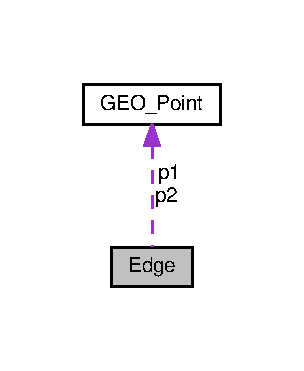
\includegraphics[width=146pt]{struct_edge__coll__graph}
\end{center}
\end{figure}
\subsection*{Data Fields}
\begin{DoxyCompactItemize}
\item 
\hyperlink{struct_g_e_o___point}{G\+E\+O\+\_\+\+Point} \hyperlink{struct_edge_aece77b6cba572ad1536ef0f6ce20cb82}{p1}
\item 
\hyperlink{struct_g_e_o___point}{G\+E\+O\+\_\+\+Point} \hyperlink{struct_edge_a51a95439187066c7cc5f32a60cdef5a6}{p2}
\end{DoxyCompactItemize}


\subsection{Detailed Description}
A straight line between two points. 

\subsection{Field Documentation}
\index{Edge@{Edge}!p1@{p1}}
\index{p1@{p1}!Edge@{Edge}}
\subsubsection[{\texorpdfstring{p1}{p1}}]{\setlength{\rightskip}{0pt plus 5cm}{\bf G\+E\+O\+\_\+\+Point} p1}\hypertarget{struct_edge_aece77b6cba572ad1536ef0f6ce20cb82}{}\label{struct_edge_aece77b6cba572ad1536ef0f6ce20cb82}
\index{Edge@{Edge}!p2@{p2}}
\index{p2@{p2}!Edge@{Edge}}
\subsubsection[{\texorpdfstring{p2}{p2}}]{\setlength{\rightskip}{0pt plus 5cm}{\bf G\+E\+O\+\_\+\+Point} p2}\hypertarget{struct_edge_a51a95439187066c7cc5f32a60cdef5a6}{}\label{struct_edge_a51a95439187066c7cc5f32a60cdef5a6}


The documentation for this struct was generated from the following file\+:\begin{DoxyCompactItemize}
\item 
src/\hyperlink{types_8h}{types.\+h}\end{DoxyCompactItemize}

\hypertarget{struct_full_g_p_s_data}{}\section{Full\+G\+P\+S\+Data Struct Reference}
\label{struct_full_g_p_s_data}\index{Full\+G\+P\+S\+Data@{Full\+G\+P\+S\+Data}}


The entire collection of relevant data, gathered from G\+PS.  




{\ttfamily \#include $<$types.\+h$>$}

\subsection*{Data Fields}
\begin{DoxyCompactItemize}
\item 
double \hyperlink{struct_full_g_p_s_data_a76714bdbc5c536fa77dfb14533ff82a9}{latitude}
\item 
double \hyperlink{struct_full_g_p_s_data_ac155e35fdeebafc89723a51520fb9fe6}{longitude}
\item 
double \hyperlink{struct_full_g_p_s_data_ae0cc66619a6d2bc3c26c6835d1165478}{lat\+\_\+deg}
\item 
double \hyperlink{struct_full_g_p_s_data_acfc9eaa9c7495fe6c9d0dae65db238a0}{lon\+\_\+deg}
\item 
unsigned char \hyperlink{struct_full_g_p_s_data_a6a2e4ad53afd61fcd716002fc2965220}{lat}
\item 
unsigned char \hyperlink{struct_full_g_p_s_data_a7e55b80071251dcef4239e60122980a4}{lon}
\item 
double \hyperlink{struct_full_g_p_s_data_a2b13d276aee0d9fd646c8fa3647e869b}{altitude}
\item 
double \hyperlink{struct_full_g_p_s_data_acaa2fde7e3fad7df8f5755347603d17b}{course}
\item 
double \hyperlink{struct_full_g_p_s_data_acdf277ddb345fbdb7ef861a9c37c290e}{spd\+Kph}
\item 
\hyperlink{types_8h_aba7bc1797add20fe3efdf37ced1182c5}{uint8\+\_\+t} \hyperlink{struct_full_g_p_s_data_a0b48c8041be823080e6346c1731a54ed}{quality}
\item 
\hyperlink{types_8h_aba7bc1797add20fe3efdf37ced1182c5}{uint8\+\_\+t} \hyperlink{struct_full_g_p_s_data_aa306fbda3e6f642c3668c299361d25d0}{satellites}
\item 
unsigned char \hyperlink{struct_full_g_p_s_data_a4217a0a41f1bf0012de0dd9daa1b8dfc}{fix\+Type}
\item 
long \hyperlink{struct_full_g_p_s_data_a820d96504a74d9f1ab7ae4d962a878ba}{fix\+Time}
\item 
double \hyperlink{struct_full_g_p_s_data_a387b6cbd184865365f92d29fd1ac32c1}{pdop}
\item 
double \hyperlink{struct_full_g_p_s_data_a7ede759392ed439219bdbac4c8ede827}{hdop}
\item 
double \hyperlink{struct_full_g_p_s_data_a4001a0f05d0c57ebdb066d738098bff7}{vdop}
\item 
double \hyperlink{struct_full_g_p_s_data_aafd79f80d0c8c393f4ddad96148f6175}{spd\+Knots}
\item 
bool \hyperlink{struct_full_g_p_s_data_ad1f0bff7112206922c9d5a87adad6f2b}{status}
\end{DoxyCompactItemize}


\subsection{Detailed Description}
The entire collection of relevant data, gathered from G\+PS. 

lat\+\_\+deg and lon\+\_\+deg are the values of a point on the map where google map would show a point. lat/lon data that\textquotesingle{}s received from N\+M\+EA sentences is in decimal, and not in degrees, hence the need for a differentiation. 

\subsection{Field Documentation}
\index{Full\+G\+P\+S\+Data@{Full\+G\+P\+S\+Data}!altitude@{altitude}}
\index{altitude@{altitude}!Full\+G\+P\+S\+Data@{Full\+G\+P\+S\+Data}}
\subsubsection[{\texorpdfstring{altitude}{altitude}}]{\setlength{\rightskip}{0pt plus 5cm}double altitude}\hypertarget{struct_full_g_p_s_data_a2b13d276aee0d9fd646c8fa3647e869b}{}\label{struct_full_g_p_s_data_a2b13d276aee0d9fd646c8fa3647e869b}
\index{Full\+G\+P\+S\+Data@{Full\+G\+P\+S\+Data}!course@{course}}
\index{course@{course}!Full\+G\+P\+S\+Data@{Full\+G\+P\+S\+Data}}
\subsubsection[{\texorpdfstring{course}{course}}]{\setlength{\rightskip}{0pt plus 5cm}double course}\hypertarget{struct_full_g_p_s_data_acaa2fde7e3fad7df8f5755347603d17b}{}\label{struct_full_g_p_s_data_acaa2fde7e3fad7df8f5755347603d17b}
\index{Full\+G\+P\+S\+Data@{Full\+G\+P\+S\+Data}!fix\+Time@{fix\+Time}}
\index{fix\+Time@{fix\+Time}!Full\+G\+P\+S\+Data@{Full\+G\+P\+S\+Data}}
\subsubsection[{\texorpdfstring{fix\+Time}{fixTime}}]{\setlength{\rightskip}{0pt plus 5cm}long fix\+Time}\hypertarget{struct_full_g_p_s_data_a820d96504a74d9f1ab7ae4d962a878ba}{}\label{struct_full_g_p_s_data_a820d96504a74d9f1ab7ae4d962a878ba}
\index{Full\+G\+P\+S\+Data@{Full\+G\+P\+S\+Data}!fix\+Type@{fix\+Type}}
\index{fix\+Type@{fix\+Type}!Full\+G\+P\+S\+Data@{Full\+G\+P\+S\+Data}}
\subsubsection[{\texorpdfstring{fix\+Type}{fixType}}]{\setlength{\rightskip}{0pt plus 5cm}unsigned char fix\+Type}\hypertarget{struct_full_g_p_s_data_a4217a0a41f1bf0012de0dd9daa1b8dfc}{}\label{struct_full_g_p_s_data_a4217a0a41f1bf0012de0dd9daa1b8dfc}
\index{Full\+G\+P\+S\+Data@{Full\+G\+P\+S\+Data}!hdop@{hdop}}
\index{hdop@{hdop}!Full\+G\+P\+S\+Data@{Full\+G\+P\+S\+Data}}
\subsubsection[{\texorpdfstring{hdop}{hdop}}]{\setlength{\rightskip}{0pt plus 5cm}double hdop}\hypertarget{struct_full_g_p_s_data_a7ede759392ed439219bdbac4c8ede827}{}\label{struct_full_g_p_s_data_a7ede759392ed439219bdbac4c8ede827}
\index{Full\+G\+P\+S\+Data@{Full\+G\+P\+S\+Data}!lat@{lat}}
\index{lat@{lat}!Full\+G\+P\+S\+Data@{Full\+G\+P\+S\+Data}}
\subsubsection[{\texorpdfstring{lat}{lat}}]{\setlength{\rightskip}{0pt plus 5cm}unsigned char lat}\hypertarget{struct_full_g_p_s_data_a6a2e4ad53afd61fcd716002fc2965220}{}\label{struct_full_g_p_s_data_a6a2e4ad53afd61fcd716002fc2965220}
\index{Full\+G\+P\+S\+Data@{Full\+G\+P\+S\+Data}!lat\+\_\+deg@{lat\+\_\+deg}}
\index{lat\+\_\+deg@{lat\+\_\+deg}!Full\+G\+P\+S\+Data@{Full\+G\+P\+S\+Data}}
\subsubsection[{\texorpdfstring{lat\+\_\+deg}{lat_deg}}]{\setlength{\rightskip}{0pt plus 5cm}double lat\+\_\+deg}\hypertarget{struct_full_g_p_s_data_ae0cc66619a6d2bc3c26c6835d1165478}{}\label{struct_full_g_p_s_data_ae0cc66619a6d2bc3c26c6835d1165478}
\index{Full\+G\+P\+S\+Data@{Full\+G\+P\+S\+Data}!latitude@{latitude}}
\index{latitude@{latitude}!Full\+G\+P\+S\+Data@{Full\+G\+P\+S\+Data}}
\subsubsection[{\texorpdfstring{latitude}{latitude}}]{\setlength{\rightskip}{0pt plus 5cm}double latitude}\hypertarget{struct_full_g_p_s_data_a76714bdbc5c536fa77dfb14533ff82a9}{}\label{struct_full_g_p_s_data_a76714bdbc5c536fa77dfb14533ff82a9}
\index{Full\+G\+P\+S\+Data@{Full\+G\+P\+S\+Data}!lon@{lon}}
\index{lon@{lon}!Full\+G\+P\+S\+Data@{Full\+G\+P\+S\+Data}}
\subsubsection[{\texorpdfstring{lon}{lon}}]{\setlength{\rightskip}{0pt plus 5cm}unsigned char lon}\hypertarget{struct_full_g_p_s_data_a7e55b80071251dcef4239e60122980a4}{}\label{struct_full_g_p_s_data_a7e55b80071251dcef4239e60122980a4}
\index{Full\+G\+P\+S\+Data@{Full\+G\+P\+S\+Data}!lon\+\_\+deg@{lon\+\_\+deg}}
\index{lon\+\_\+deg@{lon\+\_\+deg}!Full\+G\+P\+S\+Data@{Full\+G\+P\+S\+Data}}
\subsubsection[{\texorpdfstring{lon\+\_\+deg}{lon_deg}}]{\setlength{\rightskip}{0pt plus 5cm}double lon\+\_\+deg}\hypertarget{struct_full_g_p_s_data_acfc9eaa9c7495fe6c9d0dae65db238a0}{}\label{struct_full_g_p_s_data_acfc9eaa9c7495fe6c9d0dae65db238a0}
\index{Full\+G\+P\+S\+Data@{Full\+G\+P\+S\+Data}!longitude@{longitude}}
\index{longitude@{longitude}!Full\+G\+P\+S\+Data@{Full\+G\+P\+S\+Data}}
\subsubsection[{\texorpdfstring{longitude}{longitude}}]{\setlength{\rightskip}{0pt plus 5cm}double longitude}\hypertarget{struct_full_g_p_s_data_ac155e35fdeebafc89723a51520fb9fe6}{}\label{struct_full_g_p_s_data_ac155e35fdeebafc89723a51520fb9fe6}
\index{Full\+G\+P\+S\+Data@{Full\+G\+P\+S\+Data}!pdop@{pdop}}
\index{pdop@{pdop}!Full\+G\+P\+S\+Data@{Full\+G\+P\+S\+Data}}
\subsubsection[{\texorpdfstring{pdop}{pdop}}]{\setlength{\rightskip}{0pt plus 5cm}double pdop}\hypertarget{struct_full_g_p_s_data_a387b6cbd184865365f92d29fd1ac32c1}{}\label{struct_full_g_p_s_data_a387b6cbd184865365f92d29fd1ac32c1}
\index{Full\+G\+P\+S\+Data@{Full\+G\+P\+S\+Data}!quality@{quality}}
\index{quality@{quality}!Full\+G\+P\+S\+Data@{Full\+G\+P\+S\+Data}}
\subsubsection[{\texorpdfstring{quality}{quality}}]{\setlength{\rightskip}{0pt plus 5cm}{\bf uint8\+\_\+t} quality}\hypertarget{struct_full_g_p_s_data_a0b48c8041be823080e6346c1731a54ed}{}\label{struct_full_g_p_s_data_a0b48c8041be823080e6346c1731a54ed}
\index{Full\+G\+P\+S\+Data@{Full\+G\+P\+S\+Data}!satellites@{satellites}}
\index{satellites@{satellites}!Full\+G\+P\+S\+Data@{Full\+G\+P\+S\+Data}}
\subsubsection[{\texorpdfstring{satellites}{satellites}}]{\setlength{\rightskip}{0pt plus 5cm}{\bf uint8\+\_\+t} satellites}\hypertarget{struct_full_g_p_s_data_aa306fbda3e6f642c3668c299361d25d0}{}\label{struct_full_g_p_s_data_aa306fbda3e6f642c3668c299361d25d0}
number of satellites being tracked currently \index{Full\+G\+P\+S\+Data@{Full\+G\+P\+S\+Data}!spd\+Knots@{spd\+Knots}}
\index{spd\+Knots@{spd\+Knots}!Full\+G\+P\+S\+Data@{Full\+G\+P\+S\+Data}}
\subsubsection[{\texorpdfstring{spd\+Knots}{spdKnots}}]{\setlength{\rightskip}{0pt plus 5cm}double spd\+Knots}\hypertarget{struct_full_g_p_s_data_aafd79f80d0c8c393f4ddad96148f6175}{}\label{struct_full_g_p_s_data_aafd79f80d0c8c393f4ddad96148f6175}
\index{Full\+G\+P\+S\+Data@{Full\+G\+P\+S\+Data}!spd\+Kph@{spd\+Kph}}
\index{spd\+Kph@{spd\+Kph}!Full\+G\+P\+S\+Data@{Full\+G\+P\+S\+Data}}
\subsubsection[{\texorpdfstring{spd\+Kph}{spdKph}}]{\setlength{\rightskip}{0pt plus 5cm}double spd\+Kph}\hypertarget{struct_full_g_p_s_data_acdf277ddb345fbdb7ef861a9c37c290e}{}\label{struct_full_g_p_s_data_acdf277ddb345fbdb7ef861a9c37c290e}
\index{Full\+G\+P\+S\+Data@{Full\+G\+P\+S\+Data}!status@{status}}
\index{status@{status}!Full\+G\+P\+S\+Data@{Full\+G\+P\+S\+Data}}
\subsubsection[{\texorpdfstring{status}{status}}]{\setlength{\rightskip}{0pt plus 5cm}bool status}\hypertarget{struct_full_g_p_s_data_ad1f0bff7112206922c9d5a87adad6f2b}{}\label{struct_full_g_p_s_data_ad1f0bff7112206922c9d5a87adad6f2b}
\index{Full\+G\+P\+S\+Data@{Full\+G\+P\+S\+Data}!vdop@{vdop}}
\index{vdop@{vdop}!Full\+G\+P\+S\+Data@{Full\+G\+P\+S\+Data}}
\subsubsection[{\texorpdfstring{vdop}{vdop}}]{\setlength{\rightskip}{0pt plus 5cm}double vdop}\hypertarget{struct_full_g_p_s_data_a4001a0f05d0c57ebdb066d738098bff7}{}\label{struct_full_g_p_s_data_a4001a0f05d0c57ebdb066d738098bff7}


The documentation for this struct was generated from the following file\+:\begin{DoxyCompactItemize}
\item 
src/\hyperlink{types_8h}{types.\+h}\end{DoxyCompactItemize}

\hypertarget{struct_g_e_o___point}{}\section{G\+E\+O\+\_\+\+Point Struct Reference}
\label{struct_g_e_o___point}\index{G\+E\+O\+\_\+\+Point@{G\+E\+O\+\_\+\+Point}}


Represents a single 2D point.  




{\ttfamily \#include $<$types.\+h$>$}

\subsection*{Data Fields}
\begin{DoxyCompactItemize}
\item 
double \hyperlink{struct_g_e_o___point_ac155e35fdeebafc89723a51520fb9fe6}{longitude}
\item 
double \hyperlink{struct_g_e_o___point_a76714bdbc5c536fa77dfb14533ff82a9}{latitude}
\end{DoxyCompactItemize}


\subsection{Detailed Description}
Represents a single 2D point. 

\subsection{Field Documentation}
\index{G\+E\+O\+\_\+\+Point@{G\+E\+O\+\_\+\+Point}!latitude@{latitude}}
\index{latitude@{latitude}!G\+E\+O\+\_\+\+Point@{G\+E\+O\+\_\+\+Point}}
\subsubsection[{\texorpdfstring{latitude}{latitude}}]{\setlength{\rightskip}{0pt plus 5cm}double latitude}\hypertarget{struct_g_e_o___point_a76714bdbc5c536fa77dfb14533ff82a9}{}\label{struct_g_e_o___point_a76714bdbc5c536fa77dfb14533ff82a9}
\index{G\+E\+O\+\_\+\+Point@{G\+E\+O\+\_\+\+Point}!longitude@{longitude}}
\index{longitude@{longitude}!G\+E\+O\+\_\+\+Point@{G\+E\+O\+\_\+\+Point}}
\subsubsection[{\texorpdfstring{longitude}{longitude}}]{\setlength{\rightskip}{0pt plus 5cm}double longitude}\hypertarget{struct_g_e_o___point_ac155e35fdeebafc89723a51520fb9fe6}{}\label{struct_g_e_o___point_ac155e35fdeebafc89723a51520fb9fe6}


The documentation for this struct was generated from the following file\+:\begin{DoxyCompactItemize}
\item 
src/\hyperlink{types_8h}{types.\+h}\end{DoxyCompactItemize}

\hypertarget{structgga}{}\section{gga Struct Reference}
\label{structgga}\index{gga@{gga}}


Used to hold relevant data from \$\+G\+P\+G\+GA N\+M\+EA sentences from G\+PS.  




{\ttfamily \#include $<$types.\+h$>$}

\subsection*{Data Fields}
\begin{DoxyCompactItemize}
\item 
double \hyperlink{structgga_a76714bdbc5c536fa77dfb14533ff82a9}{latitude}
\item 
unsigned char \hyperlink{structgga_a6a2e4ad53afd61fcd716002fc2965220}{lat}
\item 
double \hyperlink{structgga_ac155e35fdeebafc89723a51520fb9fe6}{longitude}
\item 
unsigned char \hyperlink{structgga_a7e55b80071251dcef4239e60122980a4}{lon}
\item 
\hyperlink{types_8h_aba7bc1797add20fe3efdf37ced1182c5}{uint8\+\_\+t} \hyperlink{structgga_a0b48c8041be823080e6346c1731a54ed}{quality}
\item 
\hyperlink{types_8h_aba7bc1797add20fe3efdf37ced1182c5}{uint8\+\_\+t} \hyperlink{structgga_aa306fbda3e6f642c3668c299361d25d0}{satellites}
\item 
double \hyperlink{structgga_a2b13d276aee0d9fd646c8fa3647e869b}{altitude}
\end{DoxyCompactItemize}


\subsection{Detailed Description}
Used to hold relevant data from \$\+G\+P\+G\+GA N\+M\+EA sentences from G\+PS. 

\subsection{Field Documentation}
\index{gga@{gga}!altitude@{altitude}}
\index{altitude@{altitude}!gga@{gga}}
\subsubsection[{\texorpdfstring{altitude}{altitude}}]{\setlength{\rightskip}{0pt plus 5cm}double altitude}\hypertarget{structgga_a2b13d276aee0d9fd646c8fa3647e869b}{}\label{structgga_a2b13d276aee0d9fd646c8fa3647e869b}
\index{gga@{gga}!lat@{lat}}
\index{lat@{lat}!gga@{gga}}
\subsubsection[{\texorpdfstring{lat}{lat}}]{\setlength{\rightskip}{0pt plus 5cm}unsigned char lat}\hypertarget{structgga_a6a2e4ad53afd61fcd716002fc2965220}{}\label{structgga_a6a2e4ad53afd61fcd716002fc2965220}
\index{gga@{gga}!latitude@{latitude}}
\index{latitude@{latitude}!gga@{gga}}
\subsubsection[{\texorpdfstring{latitude}{latitude}}]{\setlength{\rightskip}{0pt plus 5cm}double latitude}\hypertarget{structgga_a76714bdbc5c536fa77dfb14533ff82a9}{}\label{structgga_a76714bdbc5c536fa77dfb14533ff82a9}
\index{gga@{gga}!lon@{lon}}
\index{lon@{lon}!gga@{gga}}
\subsubsection[{\texorpdfstring{lon}{lon}}]{\setlength{\rightskip}{0pt plus 5cm}unsigned char lon}\hypertarget{structgga_a7e55b80071251dcef4239e60122980a4}{}\label{structgga_a7e55b80071251dcef4239e60122980a4}
\index{gga@{gga}!longitude@{longitude}}
\index{longitude@{longitude}!gga@{gga}}
\subsubsection[{\texorpdfstring{longitude}{longitude}}]{\setlength{\rightskip}{0pt plus 5cm}double longitude}\hypertarget{structgga_ac155e35fdeebafc89723a51520fb9fe6}{}\label{structgga_ac155e35fdeebafc89723a51520fb9fe6}
\index{gga@{gga}!quality@{quality}}
\index{quality@{quality}!gga@{gga}}
\subsubsection[{\texorpdfstring{quality}{quality}}]{\setlength{\rightskip}{0pt plus 5cm}{\bf uint8\+\_\+t} quality}\hypertarget{structgga_a0b48c8041be823080e6346c1731a54ed}{}\label{structgga_a0b48c8041be823080e6346c1731a54ed}
\index{gga@{gga}!satellites@{satellites}}
\index{satellites@{satellites}!gga@{gga}}
\subsubsection[{\texorpdfstring{satellites}{satellites}}]{\setlength{\rightskip}{0pt plus 5cm}{\bf uint8\+\_\+t} satellites}\hypertarget{structgga_aa306fbda3e6f642c3668c299361d25d0}{}\label{structgga_aa306fbda3e6f642c3668c299361d25d0}


The documentation for this struct was generated from the following file\+:\begin{DoxyCompactItemize}
\item 
src/\hyperlink{types_8h}{types.\+h}\end{DoxyCompactItemize}

\hypertarget{structgll}{}\section{gll Struct Reference}
\label{structgll}\index{gll@{gll}}


Used to hold relevant data from \$\+G\+P\+G\+LL N\+M\+EA sentences from G\+PS.  




{\ttfamily \#include $<$types.\+h$>$}

\subsection*{Data Fields}
\begin{DoxyCompactItemize}
\item 
double \hyperlink{structgll_a76714bdbc5c536fa77dfb14533ff82a9}{latitude}
\item 
unsigned char \hyperlink{structgll_a6a2e4ad53afd61fcd716002fc2965220}{lat}
\item 
double \hyperlink{structgll_ac155e35fdeebafc89723a51520fb9fe6}{longitude}
\item 
unsigned char \hyperlink{structgll_a7e55b80071251dcef4239e60122980a4}{lon}
\item 
unsigned long \hyperlink{structgll_ac80d42f9b62a236bcb13ea2320515359}{fix\+Time}
\item 
\hyperlink{types_8h_af6a258d8f3ee5206d682d799316314b1}{bool} \hyperlink{structgll_ad1f0bff7112206922c9d5a87adad6f2b}{status}
\end{DoxyCompactItemize}


\subsection{Detailed Description}
Used to hold relevant data from \$\+G\+P\+G\+LL N\+M\+EA sentences from G\+PS. 

\subsection{Field Documentation}
\index{gll@{gll}!fix\+Time@{fix\+Time}}
\index{fix\+Time@{fix\+Time}!gll@{gll}}
\subsubsection[{\texorpdfstring{fix\+Time}{fixTime}}]{\setlength{\rightskip}{0pt plus 5cm}unsigned long fix\+Time}\hypertarget{structgll_ac80d42f9b62a236bcb13ea2320515359}{}\label{structgll_ac80d42f9b62a236bcb13ea2320515359}
\index{gll@{gll}!lat@{lat}}
\index{lat@{lat}!gll@{gll}}
\subsubsection[{\texorpdfstring{lat}{lat}}]{\setlength{\rightskip}{0pt plus 5cm}unsigned char lat}\hypertarget{structgll_a6a2e4ad53afd61fcd716002fc2965220}{}\label{structgll_a6a2e4ad53afd61fcd716002fc2965220}
\index{gll@{gll}!latitude@{latitude}}
\index{latitude@{latitude}!gll@{gll}}
\subsubsection[{\texorpdfstring{latitude}{latitude}}]{\setlength{\rightskip}{0pt plus 5cm}double latitude}\hypertarget{structgll_a76714bdbc5c536fa77dfb14533ff82a9}{}\label{structgll_a76714bdbc5c536fa77dfb14533ff82a9}
\index{gll@{gll}!lon@{lon}}
\index{lon@{lon}!gll@{gll}}
\subsubsection[{\texorpdfstring{lon}{lon}}]{\setlength{\rightskip}{0pt plus 5cm}unsigned char lon}\hypertarget{structgll_a7e55b80071251dcef4239e60122980a4}{}\label{structgll_a7e55b80071251dcef4239e60122980a4}
\index{gll@{gll}!longitude@{longitude}}
\index{longitude@{longitude}!gll@{gll}}
\subsubsection[{\texorpdfstring{longitude}{longitude}}]{\setlength{\rightskip}{0pt plus 5cm}double longitude}\hypertarget{structgll_ac155e35fdeebafc89723a51520fb9fe6}{}\label{structgll_ac155e35fdeebafc89723a51520fb9fe6}
\index{gll@{gll}!status@{status}}
\index{status@{status}!gll@{gll}}
\subsubsection[{\texorpdfstring{status}{status}}]{\setlength{\rightskip}{0pt plus 5cm}{\bf bool} status}\hypertarget{structgll_ad1f0bff7112206922c9d5a87adad6f2b}{}\label{structgll_ad1f0bff7112206922c9d5a87adad6f2b}


The documentation for this struct was generated from the following file\+:\begin{DoxyCompactItemize}
\item 
src/\hyperlink{types_8h}{types.\+h}\end{DoxyCompactItemize}

\hypertarget{struct_g_p_s___actions}{}\section{G\+P\+S\+\_\+\+Actions Struct Reference}
\label{struct_g_p_s___actions}\index{G\+P\+S\+\_\+\+Actions@{G\+P\+S\+\_\+\+Actions}}


This struct contains function pointers to functions that G\+P\+S\+Interface provides for handling gps stuff.  




{\ttfamily \#include $<$G\+P\+S\+Interface.\+h$>$}

\subsection*{Data Fields}
\begin{DoxyCompactItemize}
\item 
int($\ast$ \hyperlink{struct_g_p_s___actions_a5dd8131dc7f60bbfd44b89c1d29090b9}{get\+G\+PS} )(\hyperlink{struct_full_g_p_s_data}{Full\+G\+P\+S\+Data} $\ast$, \hyperlink{types_8h_af6a258d8f3ee5206d682d799316314b1}{bool}, void $\ast$)
\end{DoxyCompactItemize}


\subsection{Detailed Description}
This struct contains function pointers to functions that G\+P\+S\+Interface provides for handling gps stuff. 

\subsection{Field Documentation}
\index{G\+P\+S\+\_\+\+Actions@{G\+P\+S\+\_\+\+Actions}!get\+G\+PS@{get\+G\+PS}}
\index{get\+G\+PS@{get\+G\+PS}!G\+P\+S\+\_\+\+Actions@{G\+P\+S\+\_\+\+Actions}}
\subsubsection[{\texorpdfstring{get\+G\+PS}{getGPS}}]{\setlength{\rightskip}{0pt plus 5cm}int($\ast$ get\+G\+PS) ({\bf Full\+G\+P\+S\+Data} $\ast$, {\bf bool}, void $\ast$)}\hypertarget{struct_g_p_s___actions_a5dd8131dc7f60bbfd44b89c1d29090b9}{}\label{struct_g_p_s___actions_a5dd8131dc7f60bbfd44b89c1d29090b9}


The documentation for this struct was generated from the following file\+:\begin{DoxyCompactItemize}
\item 
src/\hyperlink{_g_p_s_interface_8h}{G\+P\+S\+Interface.\+h}\end{DoxyCompactItemize}

\hypertarget{struct_g_p_s_samp}{}\section{G\+P\+S\+Samp Struct Reference}
\label{struct_g_p_s_samp}\index{G\+P\+S\+Samp@{G\+P\+S\+Samp}}


Represents a smaller, truncated verion of the data gathered from G\+PS.  




{\ttfamily \#include $<$types.\+h$>$}

\subsection*{Data Fields}
\begin{DoxyCompactItemize}
\item 
double \hyperlink{struct_g_p_s_samp_a76714bdbc5c536fa77dfb14533ff82a9}{latitude}
\item 
double \hyperlink{struct_g_p_s_samp_ac155e35fdeebafc89723a51520fb9fe6}{longitude}
\item 
double \hyperlink{struct_g_p_s_samp_a6dc6e6f3c75c509ce943163afb5dade7}{speed}
\item 
double \hyperlink{struct_g_p_s_samp_a2b13d276aee0d9fd646c8fa3647e869b}{altitude}
\item 
double \hyperlink{struct_g_p_s_samp_acaa2fde7e3fad7df8f5755347603d17b}{course}
\end{DoxyCompactItemize}


\subsection{Detailed Description}
Represents a smaller, truncated verion of the data gathered from G\+PS. 

This struct contains only the most frequently used parameters. 

\subsection{Field Documentation}
\index{G\+P\+S\+Samp@{G\+P\+S\+Samp}!altitude@{altitude}}
\index{altitude@{altitude}!G\+P\+S\+Samp@{G\+P\+S\+Samp}}
\subsubsection[{\texorpdfstring{altitude}{altitude}}]{\setlength{\rightskip}{0pt plus 5cm}double altitude}\hypertarget{struct_g_p_s_samp_a2b13d276aee0d9fd646c8fa3647e869b}{}\label{struct_g_p_s_samp_a2b13d276aee0d9fd646c8fa3647e869b}
\index{G\+P\+S\+Samp@{G\+P\+S\+Samp}!course@{course}}
\index{course@{course}!G\+P\+S\+Samp@{G\+P\+S\+Samp}}
\subsubsection[{\texorpdfstring{course}{course}}]{\setlength{\rightskip}{0pt plus 5cm}double course}\hypertarget{struct_g_p_s_samp_acaa2fde7e3fad7df8f5755347603d17b}{}\label{struct_g_p_s_samp_acaa2fde7e3fad7df8f5755347603d17b}
\index{G\+P\+S\+Samp@{G\+P\+S\+Samp}!latitude@{latitude}}
\index{latitude@{latitude}!G\+P\+S\+Samp@{G\+P\+S\+Samp}}
\subsubsection[{\texorpdfstring{latitude}{latitude}}]{\setlength{\rightskip}{0pt plus 5cm}double latitude}\hypertarget{struct_g_p_s_samp_a76714bdbc5c536fa77dfb14533ff82a9}{}\label{struct_g_p_s_samp_a76714bdbc5c536fa77dfb14533ff82a9}
\index{G\+P\+S\+Samp@{G\+P\+S\+Samp}!longitude@{longitude}}
\index{longitude@{longitude}!G\+P\+S\+Samp@{G\+P\+S\+Samp}}
\subsubsection[{\texorpdfstring{longitude}{longitude}}]{\setlength{\rightskip}{0pt plus 5cm}double longitude}\hypertarget{struct_g_p_s_samp_ac155e35fdeebafc89723a51520fb9fe6}{}\label{struct_g_p_s_samp_ac155e35fdeebafc89723a51520fb9fe6}
\index{G\+P\+S\+Samp@{G\+P\+S\+Samp}!speed@{speed}}
\index{speed@{speed}!G\+P\+S\+Samp@{G\+P\+S\+Samp}}
\subsubsection[{\texorpdfstring{speed}{speed}}]{\setlength{\rightskip}{0pt plus 5cm}double speed}\hypertarget{struct_g_p_s_samp_a6dc6e6f3c75c509ce943163afb5dade7}{}\label{struct_g_p_s_samp_a6dc6e6f3c75c509ce943163afb5dade7}


The documentation for this struct was generated from the following file\+:\begin{DoxyCompactItemize}
\item 
src/\hyperlink{types_8h}{types.\+h}\end{DoxyCompactItemize}

\hypertarget{structgsa}{}\section{gsa Struct Reference}
\label{structgsa}\index{gsa@{gsa}}


Used to hold relevant data from \$\+G\+P\+G\+SA N\+M\+EA sentences from G\+PS.  




{\ttfamily \#include $<$types.\+h$>$}

\subsection*{Data Fields}
\begin{DoxyCompactItemize}
\item 
unsigned char \hyperlink{structgsa_a4217a0a41f1bf0012de0dd9daa1b8dfc}{fix\+Type}
\item 
double \hyperlink{structgsa_a387b6cbd184865365f92d29fd1ac32c1}{pdop}
\item 
double \hyperlink{structgsa_a7ede759392ed439219bdbac4c8ede827}{hdop}
\item 
double \hyperlink{structgsa_a4001a0f05d0c57ebdb066d738098bff7}{vdop}
\end{DoxyCompactItemize}


\subsection{Detailed Description}
Used to hold relevant data from \$\+G\+P\+G\+SA N\+M\+EA sentences from G\+PS. 

\subsection{Field Documentation}
\index{gsa@{gsa}!fix\+Type@{fix\+Type}}
\index{fix\+Type@{fix\+Type}!gsa@{gsa}}
\subsubsection[{\texorpdfstring{fix\+Type}{fixType}}]{\setlength{\rightskip}{0pt plus 5cm}unsigned char fix\+Type}\hypertarget{structgsa_a4217a0a41f1bf0012de0dd9daa1b8dfc}{}\label{structgsa_a4217a0a41f1bf0012de0dd9daa1b8dfc}
\index{gsa@{gsa}!hdop@{hdop}}
\index{hdop@{hdop}!gsa@{gsa}}
\subsubsection[{\texorpdfstring{hdop}{hdop}}]{\setlength{\rightskip}{0pt plus 5cm}double hdop}\hypertarget{structgsa_a7ede759392ed439219bdbac4c8ede827}{}\label{structgsa_a7ede759392ed439219bdbac4c8ede827}
\index{gsa@{gsa}!pdop@{pdop}}
\index{pdop@{pdop}!gsa@{gsa}}
\subsubsection[{\texorpdfstring{pdop}{pdop}}]{\setlength{\rightskip}{0pt plus 5cm}double pdop}\hypertarget{structgsa_a387b6cbd184865365f92d29fd1ac32c1}{}\label{structgsa_a387b6cbd184865365f92d29fd1ac32c1}
\index{gsa@{gsa}!vdop@{vdop}}
\index{vdop@{vdop}!gsa@{gsa}}
\subsubsection[{\texorpdfstring{vdop}{vdop}}]{\setlength{\rightskip}{0pt plus 5cm}double vdop}\hypertarget{structgsa_a4001a0f05d0c57ebdb066d738098bff7}{}\label{structgsa_a4001a0f05d0c57ebdb066d738098bff7}


The documentation for this struct was generated from the following file\+:\begin{DoxyCompactItemize}
\item 
src/\hyperlink{types_8h}{types.\+h}\end{DoxyCompactItemize}

\hypertarget{struct_log___master}{}\section{Log\+\_\+\+Master Struct Reference}
\label{struct_log___master}\index{Log\+\_\+\+Master@{Log\+\_\+\+Master}}


Holds all the loggers that are used to record different types of logs.  




{\ttfamily \#include $<$log\+Interface.\+h$>$}



Collaboration diagram for Log\+\_\+\+Master\+:\nopagebreak
\begin{figure}[H]
\begin{center}
\leavevmode
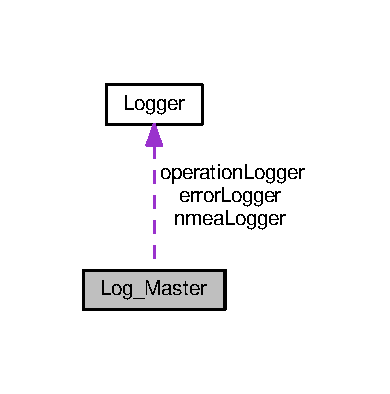
\includegraphics[width=187pt]{struct_log___master__coll__graph}
\end{center}
\end{figure}
\subsection*{Data Fields}
\begin{DoxyCompactItemize}
\item 
\hyperlink{struct_logger}{Logger} \hyperlink{struct_log___master_a86b17527dd6375131f69c50edcaa0d00}{operation\+Logger}
\item 
\hyperlink{struct_logger}{Logger} \hyperlink{struct_log___master_ad2f23f105d708487d58a08cfc0492d4a}{error\+Logger}
\item 
\hyperlink{struct_logger}{Logger} \hyperlink{struct_log___master_a39b31051fe482d807aba1796b4b0591c}{nmea\+Logger}
\end{DoxyCompactItemize}


\subsection{Detailed Description}
Holds all the loggers that are used to record different types of logs. 

\subsection{Field Documentation}
\index{Log\+\_\+\+Master@{Log\+\_\+\+Master}!error\+Logger@{error\+Logger}}
\index{error\+Logger@{error\+Logger}!Log\+\_\+\+Master@{Log\+\_\+\+Master}}
\subsubsection[{\texorpdfstring{error\+Logger}{errorLogger}}]{\setlength{\rightskip}{0pt plus 5cm}{\bf Logger} error\+Logger}\hypertarget{struct_log___master_ad2f23f105d708487d58a08cfc0492d4a}{}\label{struct_log___master_ad2f23f105d708487d58a08cfc0492d4a}
\index{Log\+\_\+\+Master@{Log\+\_\+\+Master}!nmea\+Logger@{nmea\+Logger}}
\index{nmea\+Logger@{nmea\+Logger}!Log\+\_\+\+Master@{Log\+\_\+\+Master}}
\subsubsection[{\texorpdfstring{nmea\+Logger}{nmeaLogger}}]{\setlength{\rightskip}{0pt plus 5cm}{\bf Logger} nmea\+Logger}\hypertarget{struct_log___master_a39b31051fe482d807aba1796b4b0591c}{}\label{struct_log___master_a39b31051fe482d807aba1796b4b0591c}
\index{Log\+\_\+\+Master@{Log\+\_\+\+Master}!operation\+Logger@{operation\+Logger}}
\index{operation\+Logger@{operation\+Logger}!Log\+\_\+\+Master@{Log\+\_\+\+Master}}
\subsubsection[{\texorpdfstring{operation\+Logger}{operationLogger}}]{\setlength{\rightskip}{0pt plus 5cm}{\bf Logger} operation\+Logger}\hypertarget{struct_log___master_a86b17527dd6375131f69c50edcaa0d00}{}\label{struct_log___master_a86b17527dd6375131f69c50edcaa0d00}


The documentation for this struct was generated from the following file\+:\begin{DoxyCompactItemize}
\item 
src/\hyperlink{log_interface_8h}{log\+Interface.\+h}\end{DoxyCompactItemize}

\hypertarget{struct_logger}{}\section{Logger Struct Reference}
\label{struct_logger}\index{Logger@{Logger}}


Represents a single type of logger (e.\+g. one for error, one for info, etc.)  




{\ttfamily \#include $<$log\+Interface.\+h$>$}

\subsection*{Data Fields}
\begin{DoxyCompactItemize}
\item 
F\+I\+LE $\ast$ \hyperlink{struct_logger_a3c4a30fb69c55f449605ba662e0cf5c0}{log\+File}
\item 
log4c\+\_\+category\+\_\+t $\ast$ \hyperlink{struct_logger_a58685359e8778fe049020259831b4dd2}{log\+Obj}
\item 
char $\ast$ \hyperlink{struct_logger_adac7a3f217455034b7a9cb4ae9c39a8a}{log\+Instance\+Name}
\end{DoxyCompactItemize}


\subsection{Detailed Description}
Represents a single type of logger (e.\+g. one for error, one for info, etc.) 

\subsection{Field Documentation}
\index{Logger@{Logger}!log\+File@{log\+File}}
\index{log\+File@{log\+File}!Logger@{Logger}}
\subsubsection[{\texorpdfstring{log\+File}{logFile}}]{\setlength{\rightskip}{0pt plus 5cm}F\+I\+LE$\ast$ log\+File}\hypertarget{struct_logger_a3c4a30fb69c55f449605ba662e0cf5c0}{}\label{struct_logger_a3c4a30fb69c55f449605ba662e0cf5c0}
\index{Logger@{Logger}!log\+Instance\+Name@{log\+Instance\+Name}}
\index{log\+Instance\+Name@{log\+Instance\+Name}!Logger@{Logger}}
\subsubsection[{\texorpdfstring{log\+Instance\+Name}{logInstanceName}}]{\setlength{\rightskip}{0pt plus 5cm}char$\ast$ log\+Instance\+Name}\hypertarget{struct_logger_adac7a3f217455034b7a9cb4ae9c39a8a}{}\label{struct_logger_adac7a3f217455034b7a9cb4ae9c39a8a}
\index{Logger@{Logger}!log\+Obj@{log\+Obj}}
\index{log\+Obj@{log\+Obj}!Logger@{Logger}}
\subsubsection[{\texorpdfstring{log\+Obj}{logObj}}]{\setlength{\rightskip}{0pt plus 5cm}log4c\+\_\+category\+\_\+t$\ast$ log\+Obj}\hypertarget{struct_logger_a58685359e8778fe049020259831b4dd2}{}\label{struct_logger_a58685359e8778fe049020259831b4dd2}


The documentation for this struct was generated from the following file\+:\begin{DoxyCompactItemize}
\item 
src/\hyperlink{log_interface_8h}{log\+Interface.\+h}\end{DoxyCompactItemize}

\hypertarget{struct_mavlink___messages}{}\section{Mavlink\+\_\+\+Messages Struct Reference}
\label{struct_mavlink___messages}\index{Mavlink\+\_\+\+Messages@{Mavlink\+\_\+\+Messages}}


{\ttfamily \#include $<$interface.\+h$>$}



Collaboration diagram for Mavlink\+\_\+\+Messages\+:\nopagebreak
\begin{figure}[H]
\begin{center}
\leavevmode
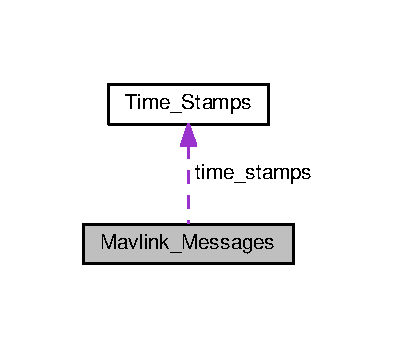
\includegraphics[width=191pt]{struct_mavlink___messages__coll__graph}
\end{center}
\end{figure}
\subsection*{Data Fields}
\begin{DoxyCompactItemize}
\item 
int \hyperlink{struct_mavlink___messages_a7a9e72f297c762c6d1b36c4c1f83a7ec}{sysid}
\item 
int \hyperlink{struct_mavlink___messages_af0d634d7b4bfadf921b2e991039d38a6}{compid}
\item 
mavlink\+\_\+heartbeat\+\_\+t \hyperlink{struct_mavlink___messages_a7ae2affcf7148de15c05eebf74909e58}{heartbeat}
\item 
mavlink\+\_\+sys\+\_\+status\+\_\+t \hyperlink{struct_mavlink___messages_ae30043ef99cf3612838c79efec1baf8d}{sys\+\_\+status}
\item 
mavlink\+\_\+battery\+\_\+status\+\_\+t \hyperlink{struct_mavlink___messages_a1d01753b58f387b8cc6d59391569dda5}{battery\+\_\+status}
\item 
mavlink\+\_\+radio\+\_\+status\+\_\+t \hyperlink{struct_mavlink___messages_a7aa8a2cdcbccb7f5696ce796e7db2194}{radio\+\_\+status}
\item 
mavlink\+\_\+local\+\_\+position\+\_\+ned\+\_\+t \hyperlink{struct_mavlink___messages_acf461f86d07049bd708dd4ac360f6da3}{local\+\_\+position\+\_\+ned}
\item 
mavlink\+\_\+global\+\_\+position\+\_\+int\+\_\+t \hyperlink{struct_mavlink___messages_a6d6095b510c6396262d76cfae41dea27}{global\+\_\+position\+\_\+int}
\item 
mavlink\+\_\+global\+\_\+position\+\_\+int\+\_\+cov\+\_\+t \hyperlink{struct_mavlink___messages_adbf6f8ee1679c7b1b6e587d437508f40}{global\+\_\+pos\+\_\+cov}
\item 
mavlink\+\_\+position\+\_\+target\+\_\+local\+\_\+ned\+\_\+t \hyperlink{struct_mavlink___messages_a1b80bbd13b6a7f75c436b16366a9bcf3}{position\+\_\+target\+\_\+local\+\_\+ned}
\item 
mavlink\+\_\+position\+\_\+target\+\_\+global\+\_\+int\+\_\+t \hyperlink{struct_mavlink___messages_ab87a0a7af2333a7fe491bbb3f44dfb29}{position\+\_\+target\+\_\+global\+\_\+int}
\item 
mavlink\+\_\+highres\+\_\+imu\+\_\+t \hyperlink{struct_mavlink___messages_afa03c0593ea0c41e2835bc771bbc7376}{highres\+\_\+imu}
\item 
mavlink\+\_\+attitude\+\_\+t \hyperlink{struct_mavlink___messages_a47b4f113f51db6752e7a800d10afffa3}{attitude}
\item 
mavlink\+\_\+command\+\_\+ack\+\_\+t \hyperlink{struct_mavlink___messages_a3ef05502567cfd552330d9ede9a89552}{command\+\_\+ack}
\item 
\hyperlink{struct_time___stamps}{Time\+\_\+\+Stamps} \hyperlink{struct_mavlink___messages_aaa9e25fa47c4a823e4d15ce2798286f1}{time\+\_\+stamps}
\end{DoxyCompactItemize}


\subsection{Detailed Description}
Holds the last messages that were received from the autopilot 

\subsection{Field Documentation}
\index{Mavlink\+\_\+\+Messages@{Mavlink\+\_\+\+Messages}!attitude@{attitude}}
\index{attitude@{attitude}!Mavlink\+\_\+\+Messages@{Mavlink\+\_\+\+Messages}}
\subsubsection[{\texorpdfstring{attitude}{attitude}}]{\setlength{\rightskip}{0pt plus 5cm}mavlink\+\_\+attitude\+\_\+t attitude}\hypertarget{struct_mavlink___messages_a47b4f113f51db6752e7a800d10afffa3}{}\label{struct_mavlink___messages_a47b4f113f51db6752e7a800d10afffa3}
\index{Mavlink\+\_\+\+Messages@{Mavlink\+\_\+\+Messages}!battery\+\_\+status@{battery\+\_\+status}}
\index{battery\+\_\+status@{battery\+\_\+status}!Mavlink\+\_\+\+Messages@{Mavlink\+\_\+\+Messages}}
\subsubsection[{\texorpdfstring{battery\+\_\+status}{battery_status}}]{\setlength{\rightskip}{0pt plus 5cm}mavlink\+\_\+battery\+\_\+status\+\_\+t battery\+\_\+status}\hypertarget{struct_mavlink___messages_a1d01753b58f387b8cc6d59391569dda5}{}\label{struct_mavlink___messages_a1d01753b58f387b8cc6d59391569dda5}
\index{Mavlink\+\_\+\+Messages@{Mavlink\+\_\+\+Messages}!command\+\_\+ack@{command\+\_\+ack}}
\index{command\+\_\+ack@{command\+\_\+ack}!Mavlink\+\_\+\+Messages@{Mavlink\+\_\+\+Messages}}
\subsubsection[{\texorpdfstring{command\+\_\+ack}{command_ack}}]{\setlength{\rightskip}{0pt plus 5cm}mavlink\+\_\+command\+\_\+ack\+\_\+t command\+\_\+ack}\hypertarget{struct_mavlink___messages_a3ef05502567cfd552330d9ede9a89552}{}\label{struct_mavlink___messages_a3ef05502567cfd552330d9ede9a89552}
\index{Mavlink\+\_\+\+Messages@{Mavlink\+\_\+\+Messages}!compid@{compid}}
\index{compid@{compid}!Mavlink\+\_\+\+Messages@{Mavlink\+\_\+\+Messages}}
\subsubsection[{\texorpdfstring{compid}{compid}}]{\setlength{\rightskip}{0pt plus 5cm}int compid}\hypertarget{struct_mavlink___messages_af0d634d7b4bfadf921b2e991039d38a6}{}\label{struct_mavlink___messages_af0d634d7b4bfadf921b2e991039d38a6}
\index{Mavlink\+\_\+\+Messages@{Mavlink\+\_\+\+Messages}!global\+\_\+pos\+\_\+cov@{global\+\_\+pos\+\_\+cov}}
\index{global\+\_\+pos\+\_\+cov@{global\+\_\+pos\+\_\+cov}!Mavlink\+\_\+\+Messages@{Mavlink\+\_\+\+Messages}}
\subsubsection[{\texorpdfstring{global\+\_\+pos\+\_\+cov}{global_pos_cov}}]{\setlength{\rightskip}{0pt plus 5cm}mavlink\+\_\+global\+\_\+position\+\_\+int\+\_\+cov\+\_\+t global\+\_\+pos\+\_\+cov}\hypertarget{struct_mavlink___messages_adbf6f8ee1679c7b1b6e587d437508f40}{}\label{struct_mavlink___messages_adbf6f8ee1679c7b1b6e587d437508f40}
\index{Mavlink\+\_\+\+Messages@{Mavlink\+\_\+\+Messages}!global\+\_\+position\+\_\+int@{global\+\_\+position\+\_\+int}}
\index{global\+\_\+position\+\_\+int@{global\+\_\+position\+\_\+int}!Mavlink\+\_\+\+Messages@{Mavlink\+\_\+\+Messages}}
\subsubsection[{\texorpdfstring{global\+\_\+position\+\_\+int}{global_position_int}}]{\setlength{\rightskip}{0pt plus 5cm}mavlink\+\_\+global\+\_\+position\+\_\+int\+\_\+t global\+\_\+position\+\_\+int}\hypertarget{struct_mavlink___messages_a6d6095b510c6396262d76cfae41dea27}{}\label{struct_mavlink___messages_a6d6095b510c6396262d76cfae41dea27}
\index{Mavlink\+\_\+\+Messages@{Mavlink\+\_\+\+Messages}!heartbeat@{heartbeat}}
\index{heartbeat@{heartbeat}!Mavlink\+\_\+\+Messages@{Mavlink\+\_\+\+Messages}}
\subsubsection[{\texorpdfstring{heartbeat}{heartbeat}}]{\setlength{\rightskip}{0pt plus 5cm}mavlink\+\_\+heartbeat\+\_\+t heartbeat}\hypertarget{struct_mavlink___messages_a7ae2affcf7148de15c05eebf74909e58}{}\label{struct_mavlink___messages_a7ae2affcf7148de15c05eebf74909e58}
\index{Mavlink\+\_\+\+Messages@{Mavlink\+\_\+\+Messages}!highres\+\_\+imu@{highres\+\_\+imu}}
\index{highres\+\_\+imu@{highres\+\_\+imu}!Mavlink\+\_\+\+Messages@{Mavlink\+\_\+\+Messages}}
\subsubsection[{\texorpdfstring{highres\+\_\+imu}{highres_imu}}]{\setlength{\rightskip}{0pt plus 5cm}mavlink\+\_\+highres\+\_\+imu\+\_\+t highres\+\_\+imu}\hypertarget{struct_mavlink___messages_afa03c0593ea0c41e2835bc771bbc7376}{}\label{struct_mavlink___messages_afa03c0593ea0c41e2835bc771bbc7376}
\index{Mavlink\+\_\+\+Messages@{Mavlink\+\_\+\+Messages}!local\+\_\+position\+\_\+ned@{local\+\_\+position\+\_\+ned}}
\index{local\+\_\+position\+\_\+ned@{local\+\_\+position\+\_\+ned}!Mavlink\+\_\+\+Messages@{Mavlink\+\_\+\+Messages}}
\subsubsection[{\texorpdfstring{local\+\_\+position\+\_\+ned}{local_position_ned}}]{\setlength{\rightskip}{0pt plus 5cm}mavlink\+\_\+local\+\_\+position\+\_\+ned\+\_\+t local\+\_\+position\+\_\+ned}\hypertarget{struct_mavlink___messages_acf461f86d07049bd708dd4ac360f6da3}{}\label{struct_mavlink___messages_acf461f86d07049bd708dd4ac360f6da3}
\index{Mavlink\+\_\+\+Messages@{Mavlink\+\_\+\+Messages}!position\+\_\+target\+\_\+global\+\_\+int@{position\+\_\+target\+\_\+global\+\_\+int}}
\index{position\+\_\+target\+\_\+global\+\_\+int@{position\+\_\+target\+\_\+global\+\_\+int}!Mavlink\+\_\+\+Messages@{Mavlink\+\_\+\+Messages}}
\subsubsection[{\texorpdfstring{position\+\_\+target\+\_\+global\+\_\+int}{position_target_global_int}}]{\setlength{\rightskip}{0pt plus 5cm}mavlink\+\_\+position\+\_\+target\+\_\+global\+\_\+int\+\_\+t position\+\_\+target\+\_\+global\+\_\+int}\hypertarget{struct_mavlink___messages_ab87a0a7af2333a7fe491bbb3f44dfb29}{}\label{struct_mavlink___messages_ab87a0a7af2333a7fe491bbb3f44dfb29}
\index{Mavlink\+\_\+\+Messages@{Mavlink\+\_\+\+Messages}!position\+\_\+target\+\_\+local\+\_\+ned@{position\+\_\+target\+\_\+local\+\_\+ned}}
\index{position\+\_\+target\+\_\+local\+\_\+ned@{position\+\_\+target\+\_\+local\+\_\+ned}!Mavlink\+\_\+\+Messages@{Mavlink\+\_\+\+Messages}}
\subsubsection[{\texorpdfstring{position\+\_\+target\+\_\+local\+\_\+ned}{position_target_local_ned}}]{\setlength{\rightskip}{0pt plus 5cm}mavlink\+\_\+position\+\_\+target\+\_\+local\+\_\+ned\+\_\+t position\+\_\+target\+\_\+local\+\_\+ned}\hypertarget{struct_mavlink___messages_a1b80bbd13b6a7f75c436b16366a9bcf3}{}\label{struct_mavlink___messages_a1b80bbd13b6a7f75c436b16366a9bcf3}
\index{Mavlink\+\_\+\+Messages@{Mavlink\+\_\+\+Messages}!radio\+\_\+status@{radio\+\_\+status}}
\index{radio\+\_\+status@{radio\+\_\+status}!Mavlink\+\_\+\+Messages@{Mavlink\+\_\+\+Messages}}
\subsubsection[{\texorpdfstring{radio\+\_\+status}{radio_status}}]{\setlength{\rightskip}{0pt plus 5cm}mavlink\+\_\+radio\+\_\+status\+\_\+t radio\+\_\+status}\hypertarget{struct_mavlink___messages_a7aa8a2cdcbccb7f5696ce796e7db2194}{}\label{struct_mavlink___messages_a7aa8a2cdcbccb7f5696ce796e7db2194}
\index{Mavlink\+\_\+\+Messages@{Mavlink\+\_\+\+Messages}!sys\+\_\+status@{sys\+\_\+status}}
\index{sys\+\_\+status@{sys\+\_\+status}!Mavlink\+\_\+\+Messages@{Mavlink\+\_\+\+Messages}}
\subsubsection[{\texorpdfstring{sys\+\_\+status}{sys_status}}]{\setlength{\rightskip}{0pt plus 5cm}mavlink\+\_\+sys\+\_\+status\+\_\+t sys\+\_\+status}\hypertarget{struct_mavlink___messages_ae30043ef99cf3612838c79efec1baf8d}{}\label{struct_mavlink___messages_ae30043ef99cf3612838c79efec1baf8d}
\index{Mavlink\+\_\+\+Messages@{Mavlink\+\_\+\+Messages}!sysid@{sysid}}
\index{sysid@{sysid}!Mavlink\+\_\+\+Messages@{Mavlink\+\_\+\+Messages}}
\subsubsection[{\texorpdfstring{sysid}{sysid}}]{\setlength{\rightskip}{0pt plus 5cm}int sysid}\hypertarget{struct_mavlink___messages_a7a9e72f297c762c6d1b36c4c1f83a7ec}{}\label{struct_mavlink___messages_a7a9e72f297c762c6d1b36c4c1f83a7ec}
\index{Mavlink\+\_\+\+Messages@{Mavlink\+\_\+\+Messages}!time\+\_\+stamps@{time\+\_\+stamps}}
\index{time\+\_\+stamps@{time\+\_\+stamps}!Mavlink\+\_\+\+Messages@{Mavlink\+\_\+\+Messages}}
\subsubsection[{\texorpdfstring{time\+\_\+stamps}{time_stamps}}]{\setlength{\rightskip}{0pt plus 5cm}{\bf Time\+\_\+\+Stamps} time\+\_\+stamps}\hypertarget{struct_mavlink___messages_aaa9e25fa47c4a823e4d15ce2798286f1}{}\label{struct_mavlink___messages_aaa9e25fa47c4a823e4d15ce2798286f1}


The documentation for this struct was generated from the following file\+:\begin{DoxyCompactItemize}
\item 
src/mavlink\+\_\+interface/inc/\hyperlink{interface_8h}{interface.\+h}\end{DoxyCompactItemize}

\hypertarget{struct_m_b_r}{}\section{M\+BR Struct Reference}
\label{struct_m_b_r}\index{M\+BR@{M\+BR}}


Minimum bounding rectangle of a certain polygon.  




{\ttfamily \#include $<$types.\+h$>$}



Collaboration diagram for M\+BR\+:\nopagebreak
\begin{figure}[H]
\begin{center}
\leavevmode
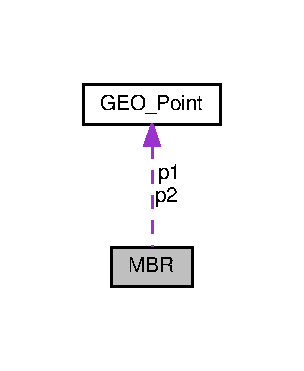
\includegraphics[width=146pt]{struct_m_b_r__coll__graph}
\end{center}
\end{figure}
\subsection*{Data Fields}
\begin{DoxyCompactItemize}
\item 
\hyperlink{struct_g_e_o___point}{G\+E\+O\+\_\+\+Point} \hyperlink{struct_m_b_r_aece77b6cba572ad1536ef0f6ce20cb82}{p1}
\item 
\hyperlink{struct_g_e_o___point}{G\+E\+O\+\_\+\+Point} \hyperlink{struct_m_b_r_a51a95439187066c7cc5f32a60cdef5a6}{p2}
\end{DoxyCompactItemize}


\subsection{Detailed Description}
Minimum bounding rectangle of a certain polygon. 

\subsection{Field Documentation}
\index{M\+BR@{M\+BR}!p1@{p1}}
\index{p1@{p1}!M\+BR@{M\+BR}}
\subsubsection[{\texorpdfstring{p1}{p1}}]{\setlength{\rightskip}{0pt plus 5cm}{\bf G\+E\+O\+\_\+\+Point} p1}\hypertarget{struct_m_b_r_aece77b6cba572ad1536ef0f6ce20cb82}{}\label{struct_m_b_r_aece77b6cba572ad1536ef0f6ce20cb82}
\index{M\+BR@{M\+BR}!p2@{p2}}
\index{p2@{p2}!M\+BR@{M\+BR}}
\subsubsection[{\texorpdfstring{p2}{p2}}]{\setlength{\rightskip}{0pt plus 5cm}{\bf G\+E\+O\+\_\+\+Point} p2}\hypertarget{struct_m_b_r_a51a95439187066c7cc5f32a60cdef5a6}{}\label{struct_m_b_r_a51a95439187066c7cc5f32a60cdef5a6}


The documentation for this struct was generated from the following file\+:\begin{DoxyCompactItemize}
\item 
src/\hyperlink{types_8h}{types.\+h}\end{DoxyCompactItemize}

\hypertarget{structrmc}{}\section{rmc Struct Reference}
\label{structrmc}\index{rmc@{rmc}}


Used to hold relevant data from \$\+G\+P\+R\+MC N\+M\+EA sentences from G\+PS.  




{\ttfamily \#include $<$types.\+h$>$}

\subsection*{Data Fields}
\begin{DoxyCompactItemize}
\item 
double \hyperlink{structrmc_a76714bdbc5c536fa77dfb14533ff82a9}{latitude}
\item 
unsigned char \hyperlink{structrmc_a6a2e4ad53afd61fcd716002fc2965220}{lat}
\item 
double \hyperlink{structrmc_ac155e35fdeebafc89723a51520fb9fe6}{longitude}
\item 
unsigned char \hyperlink{structrmc_a7e55b80071251dcef4239e60122980a4}{lon}
\item 
double \hyperlink{structrmc_a6dc6e6f3c75c509ce943163afb5dade7}{speed}
\item 
double \hyperlink{structrmc_acaa2fde7e3fad7df8f5755347603d17b}{course}
\end{DoxyCompactItemize}


\subsection{Detailed Description}
Used to hold relevant data from \$\+G\+P\+R\+MC N\+M\+EA sentences from G\+PS. 

\subsection{Field Documentation}
\index{rmc@{rmc}!course@{course}}
\index{course@{course}!rmc@{rmc}}
\subsubsection[{\texorpdfstring{course}{course}}]{\setlength{\rightskip}{0pt plus 5cm}double course}\hypertarget{structrmc_acaa2fde7e3fad7df8f5755347603d17b}{}\label{structrmc_acaa2fde7e3fad7df8f5755347603d17b}
\index{rmc@{rmc}!lat@{lat}}
\index{lat@{lat}!rmc@{rmc}}
\subsubsection[{\texorpdfstring{lat}{lat}}]{\setlength{\rightskip}{0pt plus 5cm}unsigned char lat}\hypertarget{structrmc_a6a2e4ad53afd61fcd716002fc2965220}{}\label{structrmc_a6a2e4ad53afd61fcd716002fc2965220}
\index{rmc@{rmc}!latitude@{latitude}}
\index{latitude@{latitude}!rmc@{rmc}}
\subsubsection[{\texorpdfstring{latitude}{latitude}}]{\setlength{\rightskip}{0pt plus 5cm}double latitude}\hypertarget{structrmc_a76714bdbc5c536fa77dfb14533ff82a9}{}\label{structrmc_a76714bdbc5c536fa77dfb14533ff82a9}
\index{rmc@{rmc}!lon@{lon}}
\index{lon@{lon}!rmc@{rmc}}
\subsubsection[{\texorpdfstring{lon}{lon}}]{\setlength{\rightskip}{0pt plus 5cm}unsigned char lon}\hypertarget{structrmc_a7e55b80071251dcef4239e60122980a4}{}\label{structrmc_a7e55b80071251dcef4239e60122980a4}
\index{rmc@{rmc}!longitude@{longitude}}
\index{longitude@{longitude}!rmc@{rmc}}
\subsubsection[{\texorpdfstring{longitude}{longitude}}]{\setlength{\rightskip}{0pt plus 5cm}double longitude}\hypertarget{structrmc_ac155e35fdeebafc89723a51520fb9fe6}{}\label{structrmc_ac155e35fdeebafc89723a51520fb9fe6}
\index{rmc@{rmc}!speed@{speed}}
\index{speed@{speed}!rmc@{rmc}}
\subsubsection[{\texorpdfstring{speed}{speed}}]{\setlength{\rightskip}{0pt plus 5cm}double speed}\hypertarget{structrmc_a6dc6e6f3c75c509ce943163afb5dade7}{}\label{structrmc_a6dc6e6f3c75c509ce943163afb5dade7}


The documentation for this struct was generated from the following file\+:\begin{DoxyCompactItemize}
\item 
src/\hyperlink{types_8h}{types.\+h}\end{DoxyCompactItemize}

\hypertarget{struct_time___stamps}{}\section{Time\+\_\+\+Stamps Struct Reference}
\label{struct_time___stamps}\index{Time\+\_\+\+Stamps@{Time\+\_\+\+Stamps}}


{\ttfamily \#include $<$interface.\+h$>$}

\subsection*{Data Fields}
\begin{DoxyCompactItemize}
\item 
uint64\+\_\+t \hyperlink{struct_time___stamps_a0585817e699b46e384f5ccc2d122362a}{heartbeat}
\item 
uint64\+\_\+t \hyperlink{struct_time___stamps_a0c435af1e679e794a97d29f6ad8033c4}{sys\+\_\+status}
\item 
uint64\+\_\+t \hyperlink{struct_time___stamps_af6f0cc3b4549bdc74d9f5c3b01522877}{battery\+\_\+status}
\item 
uint64\+\_\+t \hyperlink{struct_time___stamps_a349d4b854b6448bec3938af7bb59a482}{radio\+\_\+status}
\item 
uint64\+\_\+t \hyperlink{struct_time___stamps_a39f9bcf43ad658301417a7aa3ae368bd}{local\+\_\+position\+\_\+ned}
\item 
uint64\+\_\+t \hyperlink{struct_time___stamps_a9bde3d252fe8abb20df512cfb8ed1879}{global\+\_\+position\+\_\+int}
\item 
uint64\+\_\+t \hyperlink{struct_time___stamps_a90cff6c62a9d017149d202852e3c7881}{position\+\_\+target\+\_\+local\+\_\+ned}
\item 
uint64\+\_\+t \hyperlink{struct_time___stamps_a6c9893fba620cfe3b8d8ff5ffd6a375b}{position\+\_\+target\+\_\+global\+\_\+int}
\item 
uint64\+\_\+t \hyperlink{struct_time___stamps_a05ee98180378af9ae38747893f5a4561}{highres\+\_\+imu}
\item 
uint64\+\_\+t \hyperlink{struct_time___stamps_ae5c3610ce264d2ccf7f529ae494ca474}{attitude}
\item 
uint64\+\_\+t \hyperlink{struct_time___stamps_aa52d5737fe1f692528b7ff03154399ea}{command\+\_\+ack}
\end{DoxyCompactItemize}


\subsection{Field Documentation}
\index{Time\+\_\+\+Stamps@{Time\+\_\+\+Stamps}!attitude@{attitude}}
\index{attitude@{attitude}!Time\+\_\+\+Stamps@{Time\+\_\+\+Stamps}}
\subsubsection[{\texorpdfstring{attitude}{attitude}}]{\setlength{\rightskip}{0pt plus 5cm}uint64\+\_\+t attitude}\hypertarget{struct_time___stamps_ae5c3610ce264d2ccf7f529ae494ca474}{}\label{struct_time___stamps_ae5c3610ce264d2ccf7f529ae494ca474}
\index{Time\+\_\+\+Stamps@{Time\+\_\+\+Stamps}!battery\+\_\+status@{battery\+\_\+status}}
\index{battery\+\_\+status@{battery\+\_\+status}!Time\+\_\+\+Stamps@{Time\+\_\+\+Stamps}}
\subsubsection[{\texorpdfstring{battery\+\_\+status}{battery_status}}]{\setlength{\rightskip}{0pt plus 5cm}uint64\+\_\+t battery\+\_\+status}\hypertarget{struct_time___stamps_af6f0cc3b4549bdc74d9f5c3b01522877}{}\label{struct_time___stamps_af6f0cc3b4549bdc74d9f5c3b01522877}
\index{Time\+\_\+\+Stamps@{Time\+\_\+\+Stamps}!command\+\_\+ack@{command\+\_\+ack}}
\index{command\+\_\+ack@{command\+\_\+ack}!Time\+\_\+\+Stamps@{Time\+\_\+\+Stamps}}
\subsubsection[{\texorpdfstring{command\+\_\+ack}{command_ack}}]{\setlength{\rightskip}{0pt plus 5cm}uint64\+\_\+t command\+\_\+ack}\hypertarget{struct_time___stamps_aa52d5737fe1f692528b7ff03154399ea}{}\label{struct_time___stamps_aa52d5737fe1f692528b7ff03154399ea}
\index{Time\+\_\+\+Stamps@{Time\+\_\+\+Stamps}!global\+\_\+position\+\_\+int@{global\+\_\+position\+\_\+int}}
\index{global\+\_\+position\+\_\+int@{global\+\_\+position\+\_\+int}!Time\+\_\+\+Stamps@{Time\+\_\+\+Stamps}}
\subsubsection[{\texorpdfstring{global\+\_\+position\+\_\+int}{global_position_int}}]{\setlength{\rightskip}{0pt plus 5cm}uint64\+\_\+t global\+\_\+position\+\_\+int}\hypertarget{struct_time___stamps_a9bde3d252fe8abb20df512cfb8ed1879}{}\label{struct_time___stamps_a9bde3d252fe8abb20df512cfb8ed1879}
\index{Time\+\_\+\+Stamps@{Time\+\_\+\+Stamps}!heartbeat@{heartbeat}}
\index{heartbeat@{heartbeat}!Time\+\_\+\+Stamps@{Time\+\_\+\+Stamps}}
\subsubsection[{\texorpdfstring{heartbeat}{heartbeat}}]{\setlength{\rightskip}{0pt plus 5cm}uint64\+\_\+t heartbeat}\hypertarget{struct_time___stamps_a0585817e699b46e384f5ccc2d122362a}{}\label{struct_time___stamps_a0585817e699b46e384f5ccc2d122362a}
\index{Time\+\_\+\+Stamps@{Time\+\_\+\+Stamps}!highres\+\_\+imu@{highres\+\_\+imu}}
\index{highres\+\_\+imu@{highres\+\_\+imu}!Time\+\_\+\+Stamps@{Time\+\_\+\+Stamps}}
\subsubsection[{\texorpdfstring{highres\+\_\+imu}{highres_imu}}]{\setlength{\rightskip}{0pt plus 5cm}uint64\+\_\+t highres\+\_\+imu}\hypertarget{struct_time___stamps_a05ee98180378af9ae38747893f5a4561}{}\label{struct_time___stamps_a05ee98180378af9ae38747893f5a4561}
\index{Time\+\_\+\+Stamps@{Time\+\_\+\+Stamps}!local\+\_\+position\+\_\+ned@{local\+\_\+position\+\_\+ned}}
\index{local\+\_\+position\+\_\+ned@{local\+\_\+position\+\_\+ned}!Time\+\_\+\+Stamps@{Time\+\_\+\+Stamps}}
\subsubsection[{\texorpdfstring{local\+\_\+position\+\_\+ned}{local_position_ned}}]{\setlength{\rightskip}{0pt plus 5cm}uint64\+\_\+t local\+\_\+position\+\_\+ned}\hypertarget{struct_time___stamps_a39f9bcf43ad658301417a7aa3ae368bd}{}\label{struct_time___stamps_a39f9bcf43ad658301417a7aa3ae368bd}
\index{Time\+\_\+\+Stamps@{Time\+\_\+\+Stamps}!position\+\_\+target\+\_\+global\+\_\+int@{position\+\_\+target\+\_\+global\+\_\+int}}
\index{position\+\_\+target\+\_\+global\+\_\+int@{position\+\_\+target\+\_\+global\+\_\+int}!Time\+\_\+\+Stamps@{Time\+\_\+\+Stamps}}
\subsubsection[{\texorpdfstring{position\+\_\+target\+\_\+global\+\_\+int}{position_target_global_int}}]{\setlength{\rightskip}{0pt plus 5cm}uint64\+\_\+t position\+\_\+target\+\_\+global\+\_\+int}\hypertarget{struct_time___stamps_a6c9893fba620cfe3b8d8ff5ffd6a375b}{}\label{struct_time___stamps_a6c9893fba620cfe3b8d8ff5ffd6a375b}
\index{Time\+\_\+\+Stamps@{Time\+\_\+\+Stamps}!position\+\_\+target\+\_\+local\+\_\+ned@{position\+\_\+target\+\_\+local\+\_\+ned}}
\index{position\+\_\+target\+\_\+local\+\_\+ned@{position\+\_\+target\+\_\+local\+\_\+ned}!Time\+\_\+\+Stamps@{Time\+\_\+\+Stamps}}
\subsubsection[{\texorpdfstring{position\+\_\+target\+\_\+local\+\_\+ned}{position_target_local_ned}}]{\setlength{\rightskip}{0pt plus 5cm}uint64\+\_\+t position\+\_\+target\+\_\+local\+\_\+ned}\hypertarget{struct_time___stamps_a90cff6c62a9d017149d202852e3c7881}{}\label{struct_time___stamps_a90cff6c62a9d017149d202852e3c7881}
\index{Time\+\_\+\+Stamps@{Time\+\_\+\+Stamps}!radio\+\_\+status@{radio\+\_\+status}}
\index{radio\+\_\+status@{radio\+\_\+status}!Time\+\_\+\+Stamps@{Time\+\_\+\+Stamps}}
\subsubsection[{\texorpdfstring{radio\+\_\+status}{radio_status}}]{\setlength{\rightskip}{0pt plus 5cm}uint64\+\_\+t radio\+\_\+status}\hypertarget{struct_time___stamps_a349d4b854b6448bec3938af7bb59a482}{}\label{struct_time___stamps_a349d4b854b6448bec3938af7bb59a482}
\index{Time\+\_\+\+Stamps@{Time\+\_\+\+Stamps}!sys\+\_\+status@{sys\+\_\+status}}
\index{sys\+\_\+status@{sys\+\_\+status}!Time\+\_\+\+Stamps@{Time\+\_\+\+Stamps}}
\subsubsection[{\texorpdfstring{sys\+\_\+status}{sys_status}}]{\setlength{\rightskip}{0pt plus 5cm}uint64\+\_\+t sys\+\_\+status}\hypertarget{struct_time___stamps_a0c435af1e679e794a97d29f6ad8033c4}{}\label{struct_time___stamps_a0c435af1e679e794a97d29f6ad8033c4}


The documentation for this struct was generated from the following file\+:\begin{DoxyCompactItemize}
\item 
src/mavlink\+\_\+interface/inc/\hyperlink{interface_8h}{interface.\+h}\end{DoxyCompactItemize}

\hypertarget{structvtg}{}\section{vtg Struct Reference}
\label{structvtg}\index{vtg@{vtg}}


Used to hold relevant data from \$\+G\+P\+V\+TG N\+M\+EA sentences from G\+PS.  




{\ttfamily \#include $<$types.\+h$>$}

\subsection*{Data Fields}
\begin{DoxyCompactItemize}
\item 
double \hyperlink{structvtg_aafd79f80d0c8c393f4ddad96148f6175}{spd\+Knots}
\item 
double \hyperlink{structvtg_acdf277ddb345fbdb7ef861a9c37c290e}{spd\+Kph}
\end{DoxyCompactItemize}


\subsection{Detailed Description}
Used to hold relevant data from \$\+G\+P\+V\+TG N\+M\+EA sentences from G\+PS. 

\subsection{Field Documentation}
\index{vtg@{vtg}!spd\+Knots@{spd\+Knots}}
\index{spd\+Knots@{spd\+Knots}!vtg@{vtg}}
\subsubsection[{\texorpdfstring{spd\+Knots}{spdKnots}}]{\setlength{\rightskip}{0pt plus 5cm}double spd\+Knots}\hypertarget{structvtg_aafd79f80d0c8c393f4ddad96148f6175}{}\label{structvtg_aafd79f80d0c8c393f4ddad96148f6175}
\index{vtg@{vtg}!spd\+Kph@{spd\+Kph}}
\index{spd\+Kph@{spd\+Kph}!vtg@{vtg}}
\subsubsection[{\texorpdfstring{spd\+Kph}{spdKph}}]{\setlength{\rightskip}{0pt plus 5cm}double spd\+Kph}\hypertarget{structvtg_acdf277ddb345fbdb7ef861a9c37c290e}{}\label{structvtg_acdf277ddb345fbdb7ef861a9c37c290e}


The documentation for this struct was generated from the following file\+:\begin{DoxyCompactItemize}
\item 
src/\hyperlink{types_8h}{types.\+h}\end{DoxyCompactItemize}

\hypertarget{struct_zone__general}{}\section{Zone\+\_\+general Struct Reference}
\label{struct_zone__general}\index{Zone\+\_\+general@{Zone\+\_\+general}}


Represents a single polygon.  




{\ttfamily \#include $<$types.\+h$>$}



Collaboration diagram for Zone\+\_\+general\+:
\nopagebreak
\begin{figure}[H]
\begin{center}
\leavevmode
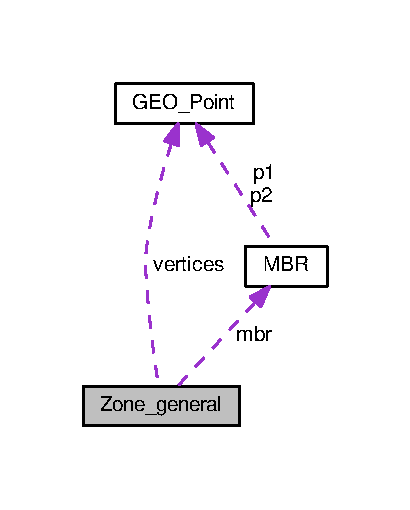
\includegraphics[width=197pt]{struct_zone__general__coll__graph}
\end{center}
\end{figure}
\subsection*{Data Fields}
\begin{DoxyCompactItemize}
\item 
size\+\_\+t \hyperlink{struct_zone__general_a4201b99044782c4891e04f4981f402e9}{num\+Vertices}
\item 
double \hyperlink{struct_zone__general_a2b13d276aee0d9fd646c8fa3647e869b}{altitude}
\item 
\hyperlink{struct_m_b_r}{M\+BR} \hyperlink{struct_zone__general_a5704de758d5631f53b2bb724b152f40b}{mbr}
\item 
\hyperlink{struct_g_e_o___point}{G\+E\+O\+\_\+\+Point} $\ast$ \hyperlink{struct_zone__general_acc847332c99d5cd8e044760a5c04fa1f}{vertices}
\end{DoxyCompactItemize}


\subsection{Detailed Description}
Represents a single polygon. 

\subsection{Field Documentation}
\index{Zone\+\_\+general@{Zone\+\_\+general}!altitude@{altitude}}
\index{altitude@{altitude}!Zone\+\_\+general@{Zone\+\_\+general}}
\subsubsection[{\texorpdfstring{altitude}{altitude}}]{\setlength{\rightskip}{0pt plus 5cm}double altitude}\hypertarget{struct_zone__general_a2b13d276aee0d9fd646c8fa3647e869b}{}\label{struct_zone__general_a2b13d276aee0d9fd646c8fa3647e869b}
\index{Zone\+\_\+general@{Zone\+\_\+general}!mbr@{mbr}}
\index{mbr@{mbr}!Zone\+\_\+general@{Zone\+\_\+general}}
\subsubsection[{\texorpdfstring{mbr}{mbr}}]{\setlength{\rightskip}{0pt plus 5cm}{\bf M\+BR} mbr}\hypertarget{struct_zone__general_a5704de758d5631f53b2bb724b152f40b}{}\label{struct_zone__general_a5704de758d5631f53b2bb724b152f40b}
\index{Zone\+\_\+general@{Zone\+\_\+general}!num\+Vertices@{num\+Vertices}}
\index{num\+Vertices@{num\+Vertices}!Zone\+\_\+general@{Zone\+\_\+general}}
\subsubsection[{\texorpdfstring{num\+Vertices}{numVertices}}]{\setlength{\rightskip}{0pt plus 5cm}size\+\_\+t num\+Vertices}\hypertarget{struct_zone__general_a4201b99044782c4891e04f4981f402e9}{}\label{struct_zone__general_a4201b99044782c4891e04f4981f402e9}
\index{Zone\+\_\+general@{Zone\+\_\+general}!vertices@{vertices}}
\index{vertices@{vertices}!Zone\+\_\+general@{Zone\+\_\+general}}
\subsubsection[{\texorpdfstring{vertices}{vertices}}]{\setlength{\rightskip}{0pt plus 5cm}{\bf G\+E\+O\+\_\+\+Point}$\ast$ vertices}\hypertarget{struct_zone__general_acc847332c99d5cd8e044760a5c04fa1f}{}\label{struct_zone__general_acc847332c99d5cd8e044760a5c04fa1f}


The documentation for this struct was generated from the following file\+:\begin{DoxyCompactItemize}
\item 
src/\hyperlink{types_8h}{types.\+h}\end{DoxyCompactItemize}

\chapter{File Documentation}
\hypertarget{autopilot__controller_8c}{}\section{src/autopilot\+\_\+controller.c File Reference}
\label{autopilot__controller_8c}\index{src/autopilot\+\_\+controller.\+c@{src/autopilot\+\_\+controller.\+c}}
{\ttfamily \#include \char`\"{}autopilot\+\_\+controller.\+h\char`\"{}}\\*
Include dependency graph for autopilot\+\_\+controller.\+c\+:\nopagebreak
\begin{figure}[H]
\begin{center}
\leavevmode
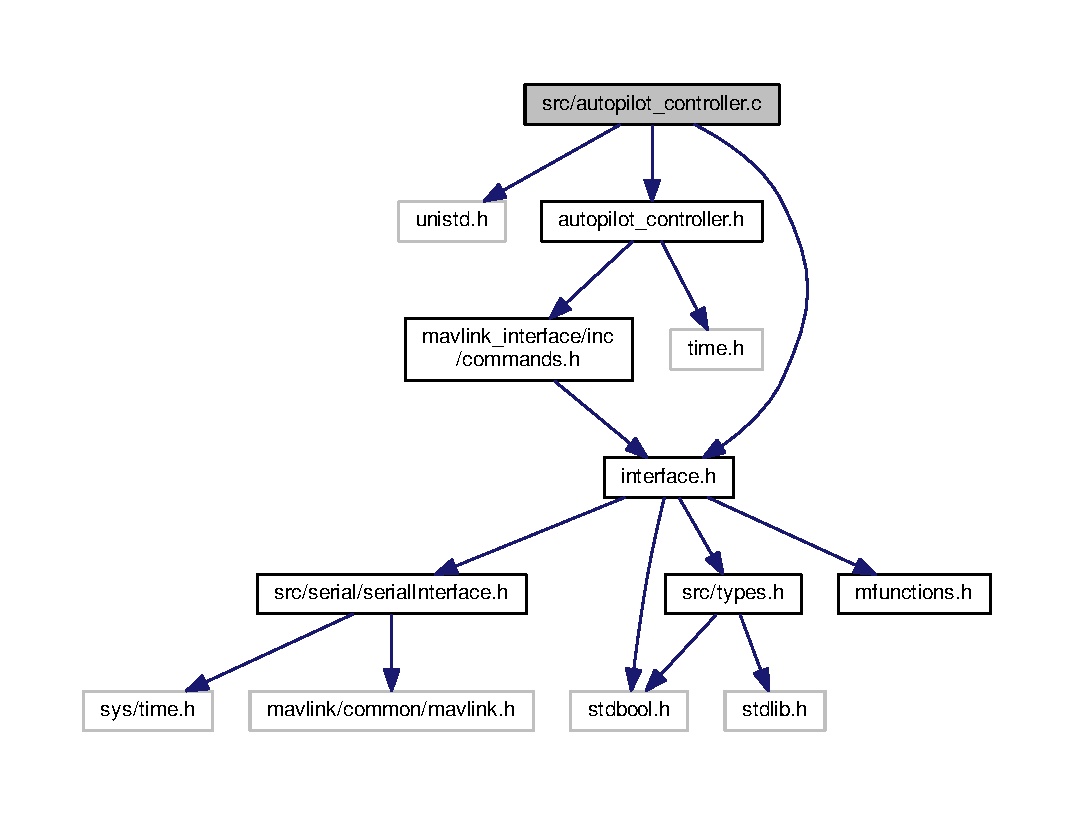
\includegraphics[width=350pt]{autopilot__controller_8c__incl}
\end{center}
\end{figure}
\subsection*{Functions}
\begin{DoxyCompactItemize}
\item 
void \hyperlink{autopilot__controller_8c_a4840fc5da500f994fe893dab4c7dbd79}{update\+\_\+autopilot} (void)
\item 
int \hyperlink{autopilot__controller_8c_aa06f4432f5f1ab850f2e7a8190d3dabd}{takeover\+\_\+control} (time\+\_\+t $\ast$commander\+Timestamp)
\end{DoxyCompactItemize}


\subsection{Function Documentation}
\index{autopilot\+\_\+controller.\+c@{autopilot\+\_\+controller.\+c}!takeover\+\_\+control@{takeover\+\_\+control}}
\index{takeover\+\_\+control@{takeover\+\_\+control}!autopilot\+\_\+controller.\+c@{autopilot\+\_\+controller.\+c}}
\subsubsection[{\texorpdfstring{takeover\+\_\+control(time\+\_\+t $\ast$commander\+Timestamp)}{takeover_control(time_t *commanderTimestamp)}}]{\setlength{\rightskip}{0pt plus 5cm}int takeover\+\_\+control (
\begin{DoxyParamCaption}
\item[{time\+\_\+t $\ast$}]{commander\+Timestamp}
\end{DoxyParamCaption}
)}\hypertarget{autopilot__controller_8c_aa06f4432f5f1ab850f2e7a8190d3dabd}{}\label{autopilot__controller_8c_aa06f4432f5f1ab850f2e7a8190d3dabd}
\index{autopilot\+\_\+controller.\+c@{autopilot\+\_\+controller.\+c}!update\+\_\+autopilot@{update\+\_\+autopilot}}
\index{update\+\_\+autopilot@{update\+\_\+autopilot}!autopilot\+\_\+controller.\+c@{autopilot\+\_\+controller.\+c}}
\subsubsection[{\texorpdfstring{update\+\_\+autopilot(void)}{update_autopilot(void)}}]{\setlength{\rightskip}{0pt plus 5cm}void update\+\_\+autopilot (
\begin{DoxyParamCaption}
\item[{void}]{}
\end{DoxyParamCaption}
)}\hypertarget{autopilot__controller_8c_a4840fc5da500f994fe893dab4c7dbd79}{}\label{autopilot__controller_8c_a4840fc5da500f994fe893dab4c7dbd79}
T\+O\+DO
\hypertarget{autopilot__controller_8d}{}\section{src/autopilot\+\_\+controller.d File Reference}
\label{autopilot__controller_8d}\index{src/autopilot\+\_\+controller.\+d@{src/autopilot\+\_\+controller.\+d}}

\hypertarget{autopilot__controller_8h}{}\section{src/autopilot\+\_\+controller.h File Reference}
\label{autopilot__controller_8h}\index{src/autopilot\+\_\+controller.\+h@{src/autopilot\+\_\+controller.\+h}}
{\ttfamily \#include $<$time.\+h$>$}\\*
{\ttfamily \#include \char`\"{}mavlink\+\_\+interface/inc/commands.\+h\char`\"{}}\\*
Include dependency graph for autopilot\+\_\+controller.\+h\+:
\nopagebreak
\begin{figure}[H]
\begin{center}
\leavevmode
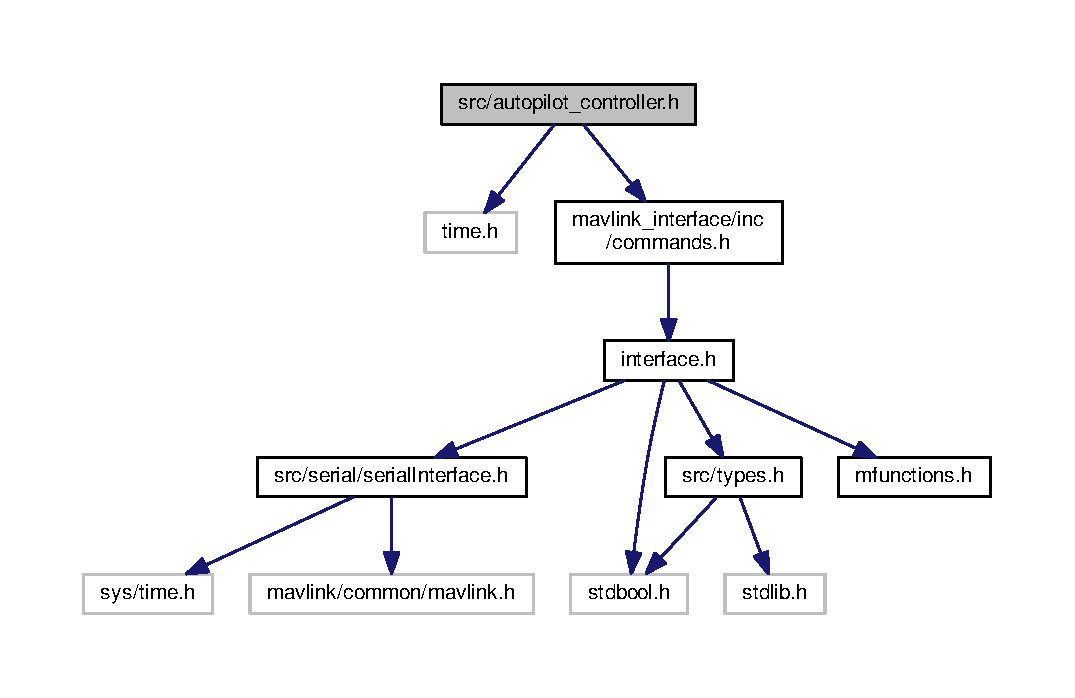
\includegraphics[width=350pt]{autopilot__controller_8h__incl}
\end{center}
\end{figure}
This graph shows which files directly or indirectly include this file\+:\nopagebreak
\begin{figure}[H]
\begin{center}
\leavevmode
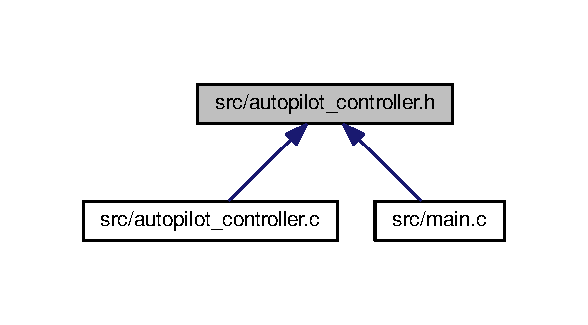
\includegraphics[width=282pt]{autopilot__controller_8h__dep__incl}
\end{center}
\end{figure}
\subsection*{Functions}
\begin{DoxyCompactItemize}
\item 
void \hyperlink{autopilot__controller_8h_a4840fc5da500f994fe893dab4c7dbd79}{update\+\_\+autopilot} (void)
\item 
int \hyperlink{autopilot__controller_8h_aa06f4432f5f1ab850f2e7a8190d3dabd}{takeover\+\_\+control} (time\+\_\+t $\ast$commander\+Timestamp)
\item 
int \hyperlink{autopilot__controller_8h_a5567c9350c378f90a37a2fb7106eb6a2}{stop\+\_\+autopilt} ()
\end{DoxyCompactItemize}


\subsection{Function Documentation}
\index{autopilot\+\_\+controller.\+h@{autopilot\+\_\+controller.\+h}!stop\+\_\+autopilt@{stop\+\_\+autopilt}}
\index{stop\+\_\+autopilt@{stop\+\_\+autopilt}!autopilot\+\_\+controller.\+h@{autopilot\+\_\+controller.\+h}}
\subsubsection[{\texorpdfstring{stop\+\_\+autopilt()}{stop_autopilt()}}]{\setlength{\rightskip}{0pt plus 5cm}int stop\+\_\+autopilt (
\begin{DoxyParamCaption}
{}
\end{DoxyParamCaption}
)}\hypertarget{autopilot__controller_8h_a5567c9350c378f90a37a2fb7106eb6a2}{}\label{autopilot__controller_8h_a5567c9350c378f90a37a2fb7106eb6a2}
\index{autopilot\+\_\+controller.\+h@{autopilot\+\_\+controller.\+h}!takeover\+\_\+control@{takeover\+\_\+control}}
\index{takeover\+\_\+control@{takeover\+\_\+control}!autopilot\+\_\+controller.\+h@{autopilot\+\_\+controller.\+h}}
\subsubsection[{\texorpdfstring{takeover\+\_\+control(time\+\_\+t $\ast$commander\+Timestamp)}{takeover_control(time_t *commanderTimestamp)}}]{\setlength{\rightskip}{0pt plus 5cm}int takeover\+\_\+control (
\begin{DoxyParamCaption}
\item[{time\+\_\+t $\ast$}]{commander\+Timestamp}
\end{DoxyParamCaption}
)}\hypertarget{autopilot__controller_8h_aa06f4432f5f1ab850f2e7a8190d3dabd}{}\label{autopilot__controller_8h_aa06f4432f5f1ab850f2e7a8190d3dabd}
\index{autopilot\+\_\+controller.\+h@{autopilot\+\_\+controller.\+h}!update\+\_\+autopilot@{update\+\_\+autopilot}}
\index{update\+\_\+autopilot@{update\+\_\+autopilot}!autopilot\+\_\+controller.\+h@{autopilot\+\_\+controller.\+h}}
\subsubsection[{\texorpdfstring{update\+\_\+autopilot(void)}{update_autopilot(void)}}]{\setlength{\rightskip}{0pt plus 5cm}void update\+\_\+autopilot (
\begin{DoxyParamCaption}
\item[{void}]{}
\end{DoxyParamCaption}
)}\hypertarget{autopilot__controller_8h_a4840fc5da500f994fe893dab4c7dbd79}{}\label{autopilot__controller_8h_a4840fc5da500f994fe893dab4c7dbd79}
T\+O\+DO
\hypertarget{gps__demo_8c}{}\section{src/\+G\+P\+S\+Demo/gps\+\_\+demo.c File Reference}
\label{gps__demo_8c}\index{src/\+G\+P\+S\+Demo/gps\+\_\+demo.\+c@{src/\+G\+P\+S\+Demo/gps\+\_\+demo.\+c}}
{\ttfamily \#include $<$stdio.\+h$>$}\\*
{\ttfamily \#include $<$math.\+h$>$}\\*
{\ttfamily \#include \char`\"{}gps\+\_\+demo.\+h\char`\"{}}\\*
{\ttfamily \#include $<$src/utils.\+h$>$}\\*
{\ttfamily \#include $<$src/log\+Interface.\+h$>$}\\*
Include dependency graph for gps\+\_\+demo.\+c\+:\nopagebreak
\begin{figure}[H]
\begin{center}
\leavevmode
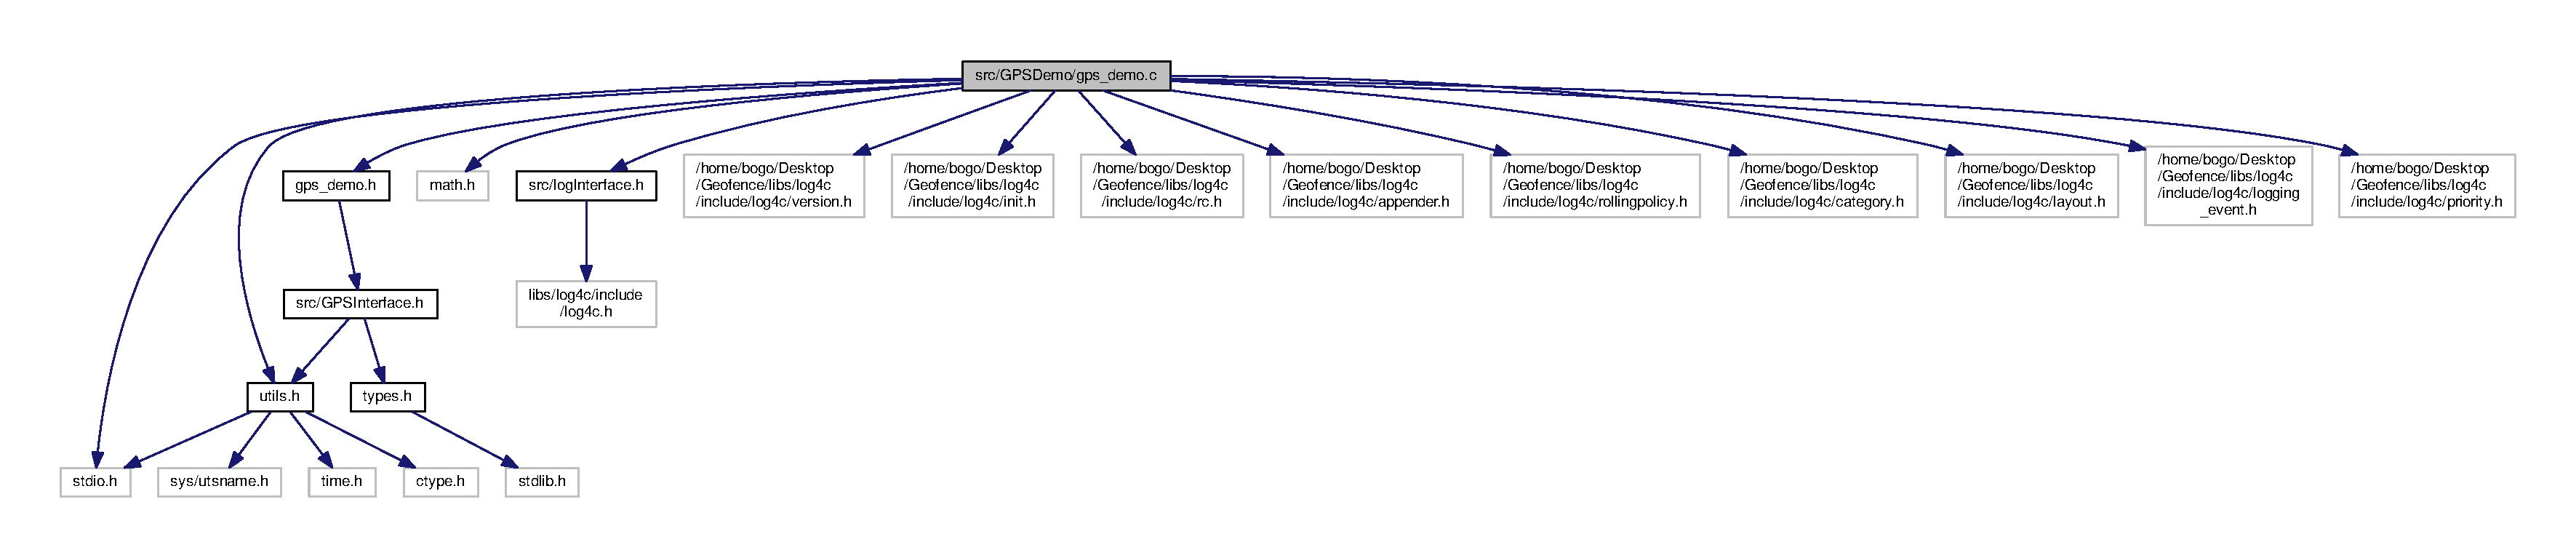
\includegraphics[width=350pt]{gps__demo_8c__incl}
\end{center}
\end{figure}
\subsection*{Functions}
\begin{DoxyCompactItemize}
\item 
int \hyperlink{gps__demo_8c_ac1e16509253fca9a2e709f4fca56316e}{get\+G\+P\+S\+Sample\+\_\+\+D\+E\+MO} (\hyperlink{struct_full_g_p_s_data}{Full\+G\+P\+S\+Data} $\ast$samp, \hyperlink{types_8h_af6a258d8f3ee5206d682d799316314b1}{bool} pass\+To\+Log, void $\ast$user\+Data)
\begin{DoxyCompactList}\small\item\em basically gets G\+PS data \end{DoxyCompactList}\end{DoxyCompactItemize}


\subsection{Function Documentation}
\index{gps\+\_\+demo.\+c@{gps\+\_\+demo.\+c}!get\+G\+P\+S\+Sample\+\_\+\+D\+E\+MO@{get\+G\+P\+S\+Sample\+\_\+\+D\+E\+MO}}
\index{get\+G\+P\+S\+Sample\+\_\+\+D\+E\+MO@{get\+G\+P\+S\+Sample\+\_\+\+D\+E\+MO}!gps\+\_\+demo.\+c@{gps\+\_\+demo.\+c}}
\subsubsection[{\texorpdfstring{get\+G\+P\+S\+Sample\+\_\+\+D\+E\+M\+O(\+Full\+G\+P\+S\+Data $\ast$samp, bool pass\+To\+Log, void $\ast$user\+Data)}{getGPSSample_DEMO(FullGPSData *samp, bool passToLog, void *userData)}}]{\setlength{\rightskip}{0pt plus 5cm}int get\+G\+P\+S\+Sample\+\_\+\+D\+E\+MO (
\begin{DoxyParamCaption}
\item[{{\bf Full\+G\+P\+S\+Data} $\ast$}]{samp, }
\item[{{\bf bool}}]{pass\+To\+Log, }
\item[{void $\ast$}]{user\+Data}
\end{DoxyParamCaption}
)}\hypertarget{gps__demo_8c_ac1e16509253fca9a2e709f4fca56316e}{}\label{gps__demo_8c_ac1e16509253fca9a2e709f4fca56316e}


basically gets G\+PS data 


\begin{DoxyParams}[1]{Parameters}
 & {\em samp} & struct with neccessary data \\
\hline
\mbox{\tt in}  & {\em pass\+To\+Log} & true if we want to log the stuff \\
\hline
\end{DoxyParams}
\begin{DoxyReturn}{Returns}
the ID of the sentence we got on this call. 
\end{DoxyReturn}

\hypertarget{gps__demo_8d}{}\section{src/\+G\+P\+S\+Demo/gps\+\_\+demo.d File Reference}
\label{gps__demo_8d}\index{src/\+G\+P\+S\+Demo/gps\+\_\+demo.\+d@{src/\+G\+P\+S\+Demo/gps\+\_\+demo.\+d}}

\hypertarget{gps__demo_8h}{}\section{src/\+G\+P\+S\+Demo/gps\+\_\+demo.h File Reference}
\label{gps__demo_8h}\index{src/\+G\+P\+S\+Demo/gps\+\_\+demo.\+h@{src/\+G\+P\+S\+Demo/gps\+\_\+demo.\+h}}
{\ttfamily \#include $<$src/\+G\+P\+S\+Interface.\+h$>$}\\*
Include dependency graph for gps\+\_\+demo.\+h\+:
\nopagebreak
\begin{figure}[H]
\begin{center}
\leavevmode
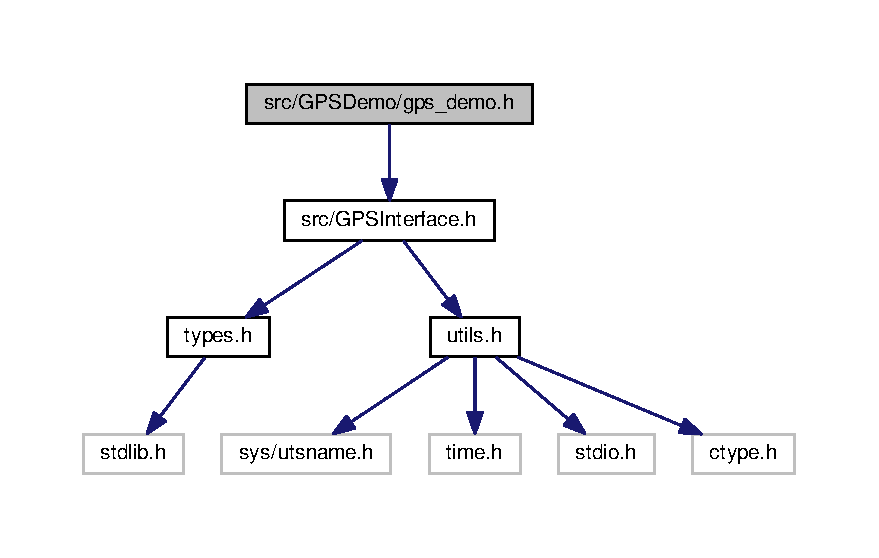
\includegraphics[width=350pt]{gps__demo_8h__incl}
\end{center}
\end{figure}
This graph shows which files directly or indirectly include this file\+:
\nopagebreak
\begin{figure}[H]
\begin{center}
\leavevmode
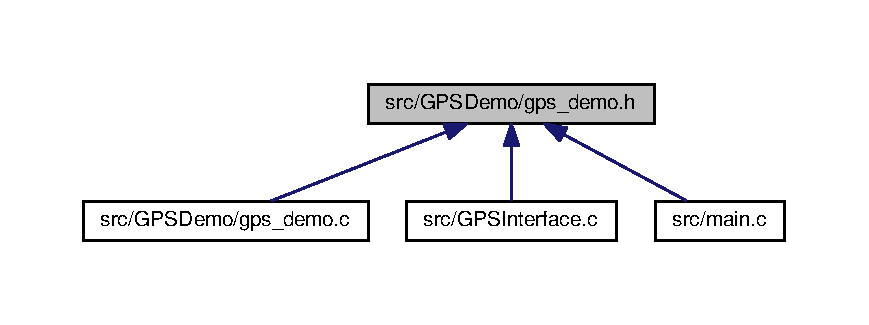
\includegraphics[width=350pt]{gps__demo_8h__dep__incl}
\end{center}
\end{figure}
\subsection*{Functions}
\begin{DoxyCompactItemize}
\item 
int \hyperlink{gps__demo_8h_ac1e16509253fca9a2e709f4fca56316e}{get\+G\+P\+S\+Sample\+\_\+\+D\+E\+MO} (\hyperlink{struct_full_g_p_s_data}{Full\+G\+P\+S\+Data} $\ast$samp, \hyperlink{types_8h_af6a258d8f3ee5206d682d799316314b1}{bool} pass\+To\+Log, void $\ast$user\+Data)
\begin{DoxyCompactList}\small\item\em basically gets G\+PS data \end{DoxyCompactList}\end{DoxyCompactItemize}


\subsection{Function Documentation}
\index{gps\+\_\+demo.\+h@{gps\+\_\+demo.\+h}!get\+G\+P\+S\+Sample\+\_\+\+D\+E\+MO@{get\+G\+P\+S\+Sample\+\_\+\+D\+E\+MO}}
\index{get\+G\+P\+S\+Sample\+\_\+\+D\+E\+MO@{get\+G\+P\+S\+Sample\+\_\+\+D\+E\+MO}!gps\+\_\+demo.\+h@{gps\+\_\+demo.\+h}}
\subsubsection[{\texorpdfstring{get\+G\+P\+S\+Sample\+\_\+\+D\+E\+M\+O(\+Full\+G\+P\+S\+Data $\ast$samp, bool pass\+To\+Log, void $\ast$user\+Data)}{getGPSSample_DEMO(FullGPSData *samp, bool passToLog, void *userData)}}]{\setlength{\rightskip}{0pt plus 5cm}int get\+G\+P\+S\+Sample\+\_\+\+D\+E\+MO (
\begin{DoxyParamCaption}
\item[{{\bf Full\+G\+P\+S\+Data} $\ast$}]{samp, }
\item[{{\bf bool}}]{pass\+To\+Log, }
\item[{void $\ast$}]{user\+Data}
\end{DoxyParamCaption}
)}\hypertarget{gps__demo_8h_ac1e16509253fca9a2e709f4fca56316e}{}\label{gps__demo_8h_ac1e16509253fca9a2e709f4fca56316e}


basically gets G\+PS data 


\begin{DoxyParams}[1]{Parameters}
 & {\em samp} & struct with neccessary data \\
\hline
\mbox{\tt in}  & {\em pass\+To\+Log} & true if we want to log the stuff \\
\hline
\end{DoxyParams}
\begin{DoxyReturn}{Returns}
the ID of the sentence we got on this call. 
\end{DoxyReturn}

\hypertarget{_g_p_s_interface_8c}{}\section{src/\+G\+P\+S\+Interface.c File Reference}
\label{_g_p_s_interface_8c}\index{src/\+G\+P\+S\+Interface.\+c@{src/\+G\+P\+S\+Interface.\+c}}
{\ttfamily \#include $<$math.\+h$>$}\\*
{\ttfamily \#include $<$string.\+h$>$}\\*
{\ttfamily \#include \char`\"{}G\+P\+S\+Interface.\+h\char`\"{}}\\*
{\ttfamily \#include \char`\"{}log\+Interface.\+h\char`\"{}}\\*
{\ttfamily \#include \char`\"{}serial/serial\+Interface.\+h\char`\"{}}\\*
{\ttfamily \#include \char`\"{}G\+P\+S\+Demo/gps\+\_\+demo.\+h\char`\"{}}\\*
Include dependency graph for G\+P\+S\+Interface.\+c\+:
\nopagebreak
\begin{figure}[H]
\begin{center}
\leavevmode
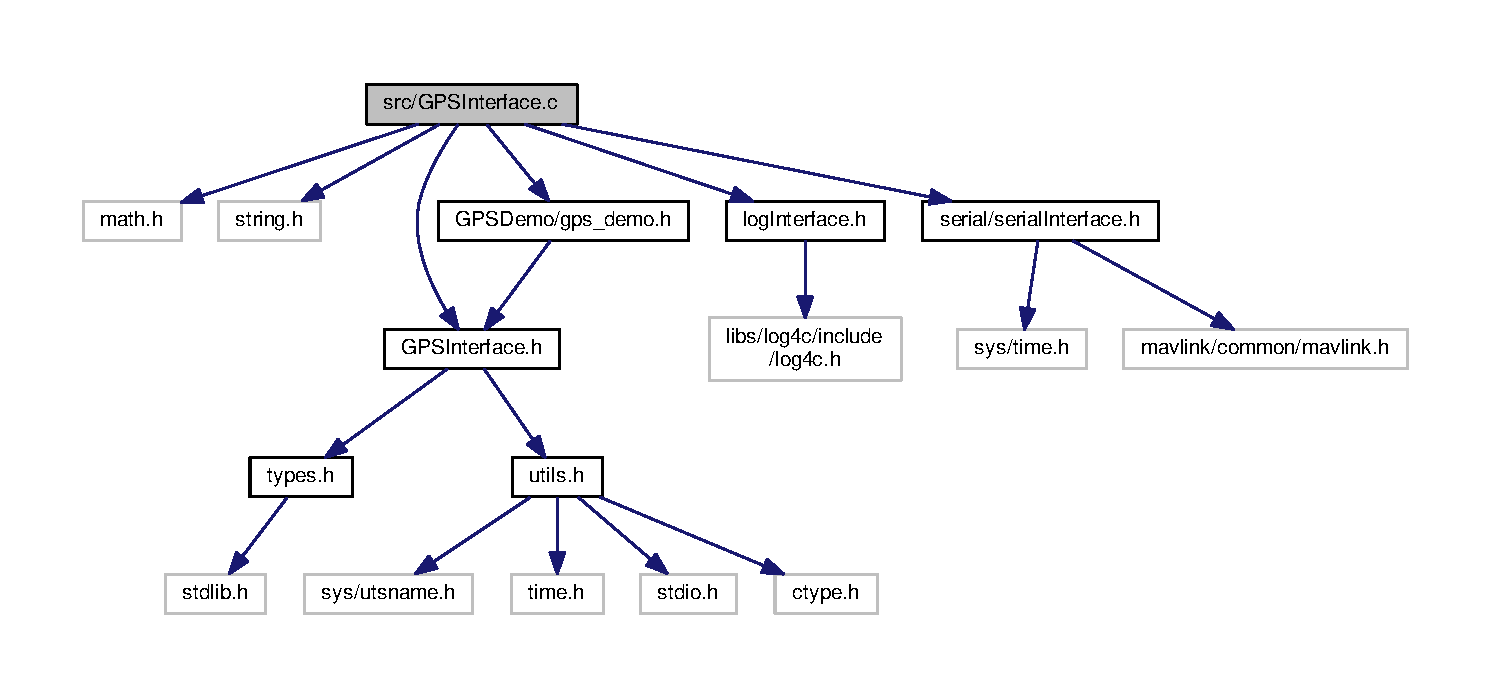
\includegraphics[width=350pt]{_g_p_s_interface_8c__incl}
\end{center}
\end{figure}
\subsection*{Functions}
\begin{DoxyCompactItemize}
\item 
int \hyperlink{_g_p_s_interface_8c_a2a940fd545a524efc707bf883f5be6a9}{G\+P\+S\+\_\+init} (\hyperlink{struct_g_p_s___actions}{G\+P\+S\+\_\+\+Actions} $\ast$gps\+Handler)
\begin{DoxyCompactList}\small\item\em assignes the correct library for the get\+G\+PS function pointer. either an R\+Pi or a demo implementation of the get\+G\+P\+S\+Sample() will be used. \end{DoxyCompactList}\item 
double \hyperlink{_g_p_s_interface_8c_a6b2e7c4d2b3a08fa15ebb18365a9264c}{to\+\_\+deg} (double x)
\begin{DoxyCompactList}\small\item\em converts N\+M\+EA decimal value to degrees (used for conversion of lat lon values) \end{DoxyCompactList}\item 
bool \hyperlink{_g_p_s_interface_8c_ac71865e68cf32819594bdcd0c4244f8d}{geofence\+\_\+breached} (\hyperlink{struct_full_g_p_s_data}{Full\+G\+P\+S\+Data} $\ast$location, \hyperlink{struct_zone__general}{Zone\+\_\+general} $\ast$zone)
\begin{DoxyCompactList}\small\item\em runs tests for different kinds of possible geofence violations, if one of the tests is failed (i.\+e some kind of violation has occured), there\textquotesingle{}s a breach. Winding Number algorithm for test of Point-\/\+In-\/\+Polygon inclusion. see \href{http://geomalgorithms.com/a03-_inclusion.html}{\tt http\+://geomalgorithms.\+com/a03-\/\+\_\+inclusion.\+html} \end{DoxyCompactList}\item 
int \hyperlink{_g_p_s_interface_8c_ac6b4d89308a2b0eab06656a5dd3d5858}{geofecnce\+\_\+alt\+\_\+check} (\hyperlink{struct_zone__general}{Zone\+\_\+general} $\ast$zone, double altitude)
\begin{DoxyCompactList}\small\item\em checks if the altitude in question is within the geofence\textquotesingle{}s height. \end{DoxyCompactList}\item 
int \hyperlink{_g_p_s_interface_8c_a74f9c1235487a3808df665a9bb7334b5}{geofence\+\_\+polygon\+\_\+check} (\hyperlink{struct_zone__general}{Zone\+\_\+general} $\ast$zone, \hyperlink{struct_g_e_o___point}{G\+E\+O\+\_\+\+Point} p)
\begin{DoxyCompactList}\small\item\em checks if the point in question is inside or outside the geofence polygon. uses the Winding-\/\+Number algorithm for test of Point-\/\+In-\/\+Polygon inclusion. see \href{http://geomalgorithms.com/a03-_inclusion.html}{\tt http\+://geomalgorithms.\+com/a03-\/\+\_\+inclusion.\+html} \end{DoxyCompactList}\item 
float \hyperlink{_g_p_s_interface_8c_a22f27d68e1909aff8c3d3f8f19be4d02}{det} (\hyperlink{struct_g_e_o___point}{G\+E\+O\+\_\+\+Point} p1, \hyperlink{struct_g_e_o___point}{G\+E\+O\+\_\+\+Point} p2, \hyperlink{struct_g_e_o___point}{G\+E\+O\+\_\+\+Point} location)
\begin{DoxyCompactList}\small\item\em the signed area of the triangle loc,P1,P2 \end{DoxyCompactList}\item 
int \hyperlink{_g_p_s_interface_8c_aa6cdb7200af7d74a9c583d5c00a50e35}{create\+\_\+edges} (\hyperlink{struct_zone__general}{Zone\+\_\+general} $\ast$zone, \hyperlink{struct_edge}{Edge} $\ast$$\ast$edges)
\begin{DoxyCompactList}\small\item\em Creates the edges of the polygon from its vertices. Called once. \end{DoxyCompactList}\item 
void \hyperlink{_g_p_s_interface_8c_a8e93b5c352c25afd3fa2aa27ae411e3a}{find\+\_\+mbr} (\hyperlink{struct_zone__general}{Zone\+\_\+general} $\ast$polygon)
\begin{DoxyCompactList}\small\item\em computes the minimum bounding rectangle of the polygon. (aka \hyperlink{struct_m_b_r}{M\+BR}) \end{DoxyCompactList}\end{DoxyCompactItemize}


\subsection{Function Documentation}
\index{G\+P\+S\+Interface.\+c@{G\+P\+S\+Interface.\+c}!create\+\_\+edges@{create\+\_\+edges}}
\index{create\+\_\+edges@{create\+\_\+edges}!G\+P\+S\+Interface.\+c@{G\+P\+S\+Interface.\+c}}
\subsubsection[{\texorpdfstring{create\+\_\+edges(\+Zone\+\_\+general $\ast$zone, Edge $\ast$$\ast$edges)}{create_edges(Zone_general *zone, Edge **edges)}}]{\setlength{\rightskip}{0pt plus 5cm}int create\+\_\+edges (
\begin{DoxyParamCaption}
\item[{{\bf Zone\+\_\+general} $\ast$}]{zone, }
\item[{{\bf Edge} $\ast$$\ast$}]{edges}
\end{DoxyParamCaption}
)}\hypertarget{_g_p_s_interface_8c_aa6cdb7200af7d74a9c583d5c00a50e35}{}\label{_g_p_s_interface_8c_aa6cdb7200af7d74a9c583d5c00a50e35}


Creates the edges of the polygon from its vertices. Called once. 


\begin{DoxyParams}{Parameters}
{\em zone} & The polygon -\/ represented by its vertices \\
\hline
{\em edges} & A \hyperlink{struct_edge}{Edge} pointer. points to an array of edges that is populated in this function \\
\hline
\end{DoxyParams}
\begin{DoxyReturn}{Returns}
returns the number of edges. (Actually returns the number of vertices). 
\end{DoxyReturn}
\index{G\+P\+S\+Interface.\+c@{G\+P\+S\+Interface.\+c}!det@{det}}
\index{det@{det}!G\+P\+S\+Interface.\+c@{G\+P\+S\+Interface.\+c}}
\subsubsection[{\texorpdfstring{det(\+G\+E\+O\+\_\+\+Point p1, G\+E\+O\+\_\+\+Point p2, G\+E\+O\+\_\+\+Point location)}{det(GEO_Point p1, GEO_Point p2, GEO_Point location)}}]{\setlength{\rightskip}{0pt plus 5cm}float det (
\begin{DoxyParamCaption}
\item[{{\bf G\+E\+O\+\_\+\+Point}}]{p1, }
\item[{{\bf G\+E\+O\+\_\+\+Point}}]{p2, }
\item[{{\bf G\+E\+O\+\_\+\+Point}}]{location}
\end{DoxyParamCaption}
)\hspace{0.3cm}{\ttfamily [inline]}}\hypertarget{_g_p_s_interface_8c_a22f27d68e1909aff8c3d3f8f19be4d02}{}\label{_g_p_s_interface_8c_a22f27d68e1909aff8c3d3f8f19be4d02}


the signed area of the triangle loc,P1,P2 

T\+O\+DO\+: inline ? 
\begin{DoxyParams}[1]{Parameters}
\mbox{\tt in}  & {\em p1} & Polygon\textquotesingle{}s first point \\
\hline
\mbox{\tt in}  & {\em p2} & Polygon\textquotesingle{}s second point \\
\hline
 & {\em location} & The query point\\
\hline
\end{DoxyParams}
\begin{DoxyReturn}{Returns}
the determinant 
\end{DoxyReturn}
\index{G\+P\+S\+Interface.\+c@{G\+P\+S\+Interface.\+c}!find\+\_\+mbr@{find\+\_\+mbr}}
\index{find\+\_\+mbr@{find\+\_\+mbr}!G\+P\+S\+Interface.\+c@{G\+P\+S\+Interface.\+c}}
\subsubsection[{\texorpdfstring{find\+\_\+mbr(\+Zone\+\_\+general $\ast$polygon)}{find_mbr(Zone_general *polygon)}}]{\setlength{\rightskip}{0pt plus 5cm}void find\+\_\+mbr (
\begin{DoxyParamCaption}
\item[{{\bf Zone\+\_\+general} $\ast$}]{polygon}
\end{DoxyParamCaption}
)}\hypertarget{_g_p_s_interface_8c_a8e93b5c352c25afd3fa2aa27ae411e3a}{}\label{_g_p_s_interface_8c_a8e93b5c352c25afd3fa2aa27ae411e3a}


computes the minimum bounding rectangle of the polygon. (aka \hyperlink{struct_m_b_r}{M\+BR}) 


\begin{DoxyParams}{Parameters}
{\em polygon} & a struct with the polygon\textquotesingle{}s points. \\
\hline
\end{DoxyParams}
\index{G\+P\+S\+Interface.\+c@{G\+P\+S\+Interface.\+c}!geofecnce\+\_\+alt\+\_\+check@{geofecnce\+\_\+alt\+\_\+check}}
\index{geofecnce\+\_\+alt\+\_\+check@{geofecnce\+\_\+alt\+\_\+check}!G\+P\+S\+Interface.\+c@{G\+P\+S\+Interface.\+c}}
\subsubsection[{\texorpdfstring{geofecnce\+\_\+alt\+\_\+check(\+Zone\+\_\+general $\ast$zone, double altitude)}{geofecnce_alt_check(Zone_general *zone, double altitude)}}]{\setlength{\rightskip}{0pt plus 5cm}int geofecnce\+\_\+alt\+\_\+check (
\begin{DoxyParamCaption}
\item[{{\bf Zone\+\_\+general} $\ast$}]{zone, }
\item[{double}]{altitude}
\end{DoxyParamCaption}
)}\hypertarget{_g_p_s_interface_8c_ac6b4d89308a2b0eab06656a5dd3d5858}{}\label{_g_p_s_interface_8c_ac6b4d89308a2b0eab06656a5dd3d5858}


checks if the altitude in question is within the geofence\textquotesingle{}s height. 

T\+O\+DO\+: min and max alt. 
\begin{DoxyParams}[1]{Parameters}
 & {\em zone} & The Polygon. the \hyperlink{struct_zone__general}{Zone\+\_\+general} struct contains the limit altitude \\
\hline
\mbox{\tt in}  & {\em altitude} & The altitude of the point in question.\\
\hline
\end{DoxyParams}
\begin{DoxyReturn}{Returns}
one of the constants describing the status, according to the outcome of the height test. 
\end{DoxyReturn}
\index{G\+P\+S\+Interface.\+c@{G\+P\+S\+Interface.\+c}!geofence\+\_\+breached@{geofence\+\_\+breached}}
\index{geofence\+\_\+breached@{geofence\+\_\+breached}!G\+P\+S\+Interface.\+c@{G\+P\+S\+Interface.\+c}}
\subsubsection[{\texorpdfstring{geofence\+\_\+breached(\+Full\+G\+P\+S\+Data $\ast$location, Zone\+\_\+general $\ast$zone)}{geofence_breached(FullGPSData *location, Zone_general *zone)}}]{\setlength{\rightskip}{0pt plus 5cm}bool geofence\+\_\+breached (
\begin{DoxyParamCaption}
\item[{{\bf Full\+G\+P\+S\+Data} $\ast$}]{location, }
\item[{{\bf Zone\+\_\+general} $\ast$}]{zone}
\end{DoxyParamCaption}
)}\hypertarget{_g_p_s_interface_8c_ac71865e68cf32819594bdcd0c4244f8d}{}\label{_g_p_s_interface_8c_ac71865e68cf32819594bdcd0c4244f8d}


runs tests for different kinds of possible geofence violations, if one of the tests is failed (i.\+e some kind of violation has occured), there\textquotesingle{}s a breach. Winding Number algorithm for test of Point-\/\+In-\/\+Polygon inclusion. see \href{http://geomalgorithms.com/a03-_inclusion.html}{\tt http\+://geomalgorithms.\+com/a03-\/\+\_\+inclusion.\+html} 


\begin{DoxyParams}{Parameters}
{\em location} & the location of the test points (coordinates) \\
\hline
{\em zone} & the Polygon -\/ represented by its vertices \\
\hline
\end{DoxyParams}
\begin{DoxyReturn}{Returns}
returns true if the point is inside the polygon. if the point is inside the polygon, the winding number is non-\/zero. a detailed description of the algorithm is in the link. 
\end{DoxyReturn}
T\+O\+DO\+: differentiate between W\+GS and M\+SL. T\+O\+DO\+: check for minimum altitude ?\index{G\+P\+S\+Interface.\+c@{G\+P\+S\+Interface.\+c}!geofence\+\_\+polygon\+\_\+check@{geofence\+\_\+polygon\+\_\+check}}
\index{geofence\+\_\+polygon\+\_\+check@{geofence\+\_\+polygon\+\_\+check}!G\+P\+S\+Interface.\+c@{G\+P\+S\+Interface.\+c}}
\subsubsection[{\texorpdfstring{geofence\+\_\+polygon\+\_\+check(\+Zone\+\_\+general $\ast$zone, G\+E\+O\+\_\+\+Point p)}{geofence_polygon_check(Zone_general *zone, GEO_Point p)}}]{\setlength{\rightskip}{0pt plus 5cm}int geofence\+\_\+polygon\+\_\+check (
\begin{DoxyParamCaption}
\item[{{\bf Zone\+\_\+general} $\ast$}]{zone, }
\item[{{\bf G\+E\+O\+\_\+\+Point}}]{p}
\end{DoxyParamCaption}
)}\hypertarget{_g_p_s_interface_8c_a74f9c1235487a3808df665a9bb7334b5}{}\label{_g_p_s_interface_8c_a74f9c1235487a3808df665a9bb7334b5}


checks if the point in question is inside or outside the geofence polygon. uses the Winding-\/\+Number algorithm for test of Point-\/\+In-\/\+Polygon inclusion. see \href{http://geomalgorithms.com/a03-_inclusion.html}{\tt http\+://geomalgorithms.\+com/a03-\/\+\_\+inclusion.\+html} 


\begin{DoxyParams}[1]{Parameters}
 & {\em zone} & The geofence polygon \\
\hline
\mbox{\tt in}  & {\em p} & the P\+OI \\
\hline
\end{DoxyParams}
\begin{DoxyReturn}{Returns}
one of the constants describing the status, according to the outcome of the PiP test. 
\end{DoxyReturn}
\index{G\+P\+S\+Interface.\+c@{G\+P\+S\+Interface.\+c}!G\+P\+S\+\_\+init@{G\+P\+S\+\_\+init}}
\index{G\+P\+S\+\_\+init@{G\+P\+S\+\_\+init}!G\+P\+S\+Interface.\+c@{G\+P\+S\+Interface.\+c}}
\subsubsection[{\texorpdfstring{G\+P\+S\+\_\+init(\+G\+P\+S\+\_\+\+Actions $\ast$gps\+Handler)}{GPS_init(GPS_Actions *gpsHandler)}}]{\setlength{\rightskip}{0pt plus 5cm}int G\+P\+S\+\_\+init (
\begin{DoxyParamCaption}
\item[{{\bf G\+P\+S\+\_\+\+Actions} $\ast$}]{gps\+Handler}
\end{DoxyParamCaption}
)}\hypertarget{_g_p_s_interface_8c_a2a940fd545a524efc707bf883f5be6a9}{}\label{_g_p_s_interface_8c_a2a940fd545a524efc707bf883f5be6a9}


assignes the correct library for the get\+G\+PS function pointer. either an R\+Pi or a demo implementation of the get\+G\+P\+S\+Sample() will be used. 

\begin{DoxyReturn}{Returns}
0 on success. 
\end{DoxyReturn}
\index{G\+P\+S\+Interface.\+c@{G\+P\+S\+Interface.\+c}!to\+\_\+deg@{to\+\_\+deg}}
\index{to\+\_\+deg@{to\+\_\+deg}!G\+P\+S\+Interface.\+c@{G\+P\+S\+Interface.\+c}}
\subsubsection[{\texorpdfstring{to\+\_\+deg(double x)}{to_deg(double x)}}]{\setlength{\rightskip}{0pt plus 5cm}double to\+\_\+deg (
\begin{DoxyParamCaption}
\item[{double}]{x}
\end{DoxyParamCaption}
)}\hypertarget{_g_p_s_interface_8c_a6b2e7c4d2b3a08fa15ebb18365a9264c}{}\label{_g_p_s_interface_8c_a6b2e7c4d2b3a08fa15ebb18365a9264c}


converts N\+M\+EA decimal value to degrees (used for conversion of lat lon values) 


\begin{DoxyParams}[1]{Parameters}
\mbox{\tt in}  & {\em x} & the decimal value extracted as-\/is from N\+M\+EA \\
\hline
\end{DoxyParams}
\begin{DoxyReturn}{Returns}
a value converted from dec to deg 
\end{DoxyReturn}

\hypertarget{_g_p_s_interface_8d}{}\section{src/\+G\+P\+S\+Interface.d File Reference}
\label{_g_p_s_interface_8d}\index{src/\+G\+P\+S\+Interface.\+d@{src/\+G\+P\+S\+Interface.\+d}}

\hypertarget{_g_p_s_interface_8h}{}\section{src/\+G\+P\+S\+Interface.h File Reference}
\label{_g_p_s_interface_8h}\index{src/\+G\+P\+S\+Interface.\+h@{src/\+G\+P\+S\+Interface.\+h}}
{\ttfamily \#include \char`\"{}types.\+h\char`\"{}}\\*
{\ttfamily \#include \char`\"{}utils.\+h\char`\"{}}\\*
Include dependency graph for G\+P\+S\+Interface.\+h\+:
\nopagebreak
\begin{figure}[H]
\begin{center}
\leavevmode
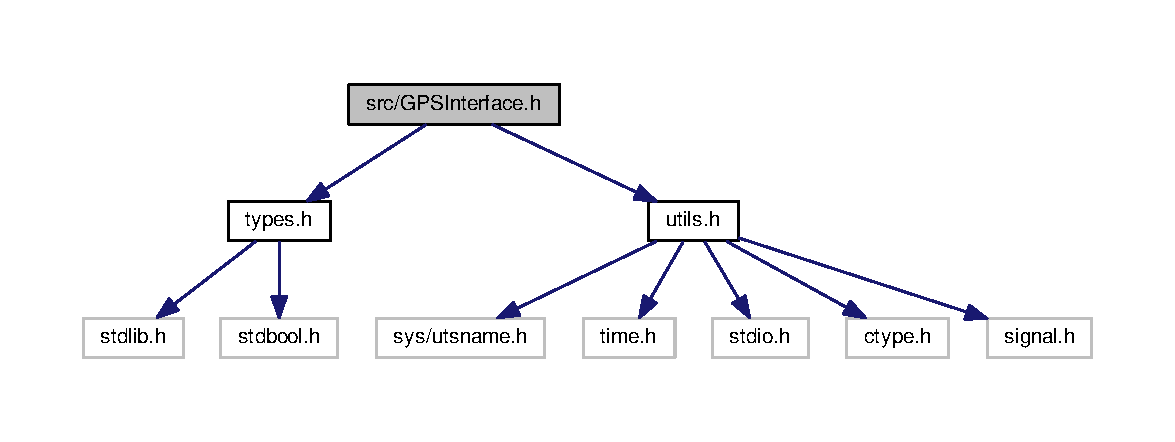
\includegraphics[width=350pt]{_g_p_s_interface_8h__incl}
\end{center}
\end{figure}
This graph shows which files directly or indirectly include this file\+:
\nopagebreak
\begin{figure}[H]
\begin{center}
\leavevmode
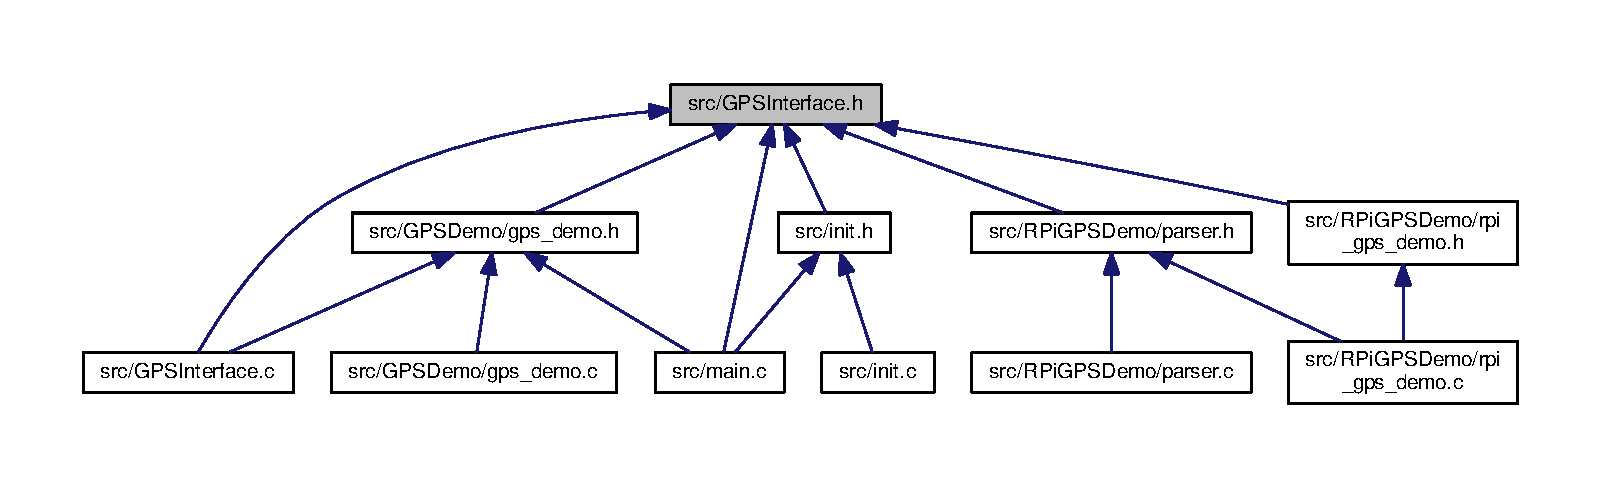
\includegraphics[width=350pt]{_g_p_s_interface_8h__dep__incl}
\end{center}
\end{figure}
\subsection*{Data Structures}
\begin{DoxyCompactItemize}
\item 
struct \hyperlink{struct_g_p_s___actions}{G\+P\+S\+\_\+\+Actions}
\begin{DoxyCompactList}\small\item\em This struct contains function pointers to functions that G\+P\+S\+Interface provides for handling gps stuff. \end{DoxyCompactList}\end{DoxyCompactItemize}
\subsection*{Macros}
\begin{DoxyCompactItemize}
\item 
\#define \hyperlink{_g_p_s_interface_8h_a4692f468d85af5af46c57358e7ecc272}{F\+U\+L\+L\+\_\+\+S\+A\+M\+P\+LE}~1
\item 
\#define \hyperlink{_g_p_s_interface_8h_a619035b765bd6e42c8da0e4c9250b111}{R\+E\+G\+I\+S\+T\+E\+R\+E\+D\+\_\+\+G\+GA}~2
\item 
\#define \hyperlink{_g_p_s_interface_8h_addbe2e6252c0483adc9c7bcd70d971d6}{R\+E\+G\+I\+S\+T\+E\+R\+E\+D\+\_\+\+R\+MC}~3
\item 
\#define \hyperlink{_g_p_s_interface_8h_aa7df72ae29c9dd2729846155947f7011}{R\+E\+G\+I\+S\+T\+E\+R\+E\+D\+\_\+\+G\+SA}~4
\item 
\#define \hyperlink{_g_p_s_interface_8h_a72557c85b2538ada64995745db824b83}{R\+E\+G\+I\+S\+T\+E\+R\+E\+D\+\_\+\+V\+TG}~5
\item 
\#define \hyperlink{_g_p_s_interface_8h_a03369e09065b63a074c1003ec9f6c285}{R\+E\+G\+I\+S\+T\+E\+R\+E\+D\+\_\+\+G\+LL}~6
\item 
\#define \hyperlink{_g_p_s_interface_8h_a04b5c325e478a8ac711eace85fd7e25d}{I\+G\+N\+O\+R\+E\+D\+\_\+\+T\+XT}~9
\item 
\#define \hyperlink{_g_p_s_interface_8h_a8e14dc82616e2c50a182cb83ba5cd8b0}{U\+N\+R\+E\+C\+O\+G\+N\+I\+Z\+E\+D\+\_\+\+N\+M\+EA}~-\/1
\item 
\#define \hyperlink{_g_p_s_interface_8h_a4519bcd8e318aa939aebe4633f4e90f0}{G\+E\+O\+F\+E\+N\+C\+E\+\_\+\+A\+L\+T\+\_\+\+OK}~10
\item 
\#define \hyperlink{_g_p_s_interface_8h_ab39428244337fd6085198cc6a9d8db14}{G\+E\+O\+F\+E\+N\+C\+E\+\_\+\+A\+L\+T\+\_\+\+B\+R\+E\+A\+CH}~100
\item 
\#define \hyperlink{_g_p_s_interface_8h_a962c38fae72cbb5bae7a59ec71645c15}{G\+E\+O\+F\+E\+N\+C\+E\+\_\+\+P\+O\+L\+Y\+G\+O\+N\+\_\+\+OK}~20
\item 
\#define \hyperlink{_g_p_s_interface_8h_a542c590073b5d5a0af9d6d72931cd835}{G\+E\+O\+F\+E\+N\+C\+E\+\_\+\+P\+O\+L\+Y\+G\+O\+N\+\_\+\+B\+R\+E\+A\+CH}~200
\end{DoxyCompactItemize}
\subsection*{Typedefs}
\begin{DoxyCompactItemize}
\item 
typedef struct \hyperlink{struct_g_p_s___actions}{G\+P\+S\+\_\+\+Actions} \hyperlink{_g_p_s_interface_8h_abe4803ce5a9fadb1eb6eaa06414d4b83}{G\+P\+S\+\_\+\+Actions}
\end{DoxyCompactItemize}
\subsection*{Functions}
\begin{DoxyCompactItemize}
\item 
float \hyperlink{_g_p_s_interface_8h_a22f27d68e1909aff8c3d3f8f19be4d02}{det} (\hyperlink{struct_g_e_o___point}{G\+E\+O\+\_\+\+Point} p1, \hyperlink{struct_g_e_o___point}{G\+E\+O\+\_\+\+Point} p2, \hyperlink{struct_g_e_o___point}{G\+E\+O\+\_\+\+Point} location)
\begin{DoxyCompactList}\small\item\em the signed area of the triangle loc,P1,P2 \end{DoxyCompactList}\item 
int \hyperlink{_g_p_s_interface_8h_a2a940fd545a524efc707bf883f5be6a9}{G\+P\+S\+\_\+init} (\hyperlink{struct_g_p_s___actions}{G\+P\+S\+\_\+\+Actions} $\ast$gps\+Handler)
\begin{DoxyCompactList}\small\item\em assignes the correct library for the get\+G\+PS function pointer. either an R\+Pi or a demo implementation of the get\+G\+P\+S\+Sample() will be used. \end{DoxyCompactList}\item 
\hyperlink{types_8h_af6a258d8f3ee5206d682d799316314b1}{bool} \hyperlink{_g_p_s_interface_8h_ac71865e68cf32819594bdcd0c4244f8d}{geofence\+\_\+breached} (\hyperlink{struct_full_g_p_s_data}{Full\+G\+P\+S\+Data} $\ast$location, \hyperlink{struct_zone__general}{Zone\+\_\+general} $\ast$zone)
\begin{DoxyCompactList}\small\item\em runs tests for different kinds of possible geofence violations, if one of the tests is failed (i.\+e some kind of violation has occured), there\textquotesingle{}s a breach. Winding Number algorithm for test of Point-\/\+In-\/\+Polygon inclusion. see \href{http://geomalgorithms.com/a03-_inclusion.html}{\tt http\+://geomalgorithms.\+com/a03-\/\+\_\+inclusion.\+html} \end{DoxyCompactList}\item 
int \hyperlink{_g_p_s_interface_8h_ac6b4d89308a2b0eab06656a5dd3d5858}{geofecnce\+\_\+alt\+\_\+check} (\hyperlink{struct_zone__general}{Zone\+\_\+general} $\ast$zone, double altitude)
\begin{DoxyCompactList}\small\item\em checks if the altitude in question is within the geofence\textquotesingle{}s height. \end{DoxyCompactList}\item 
int \hyperlink{_g_p_s_interface_8h_a74f9c1235487a3808df665a9bb7334b5}{geofence\+\_\+polygon\+\_\+check} (\hyperlink{struct_zone__general}{Zone\+\_\+general} $\ast$zone, \hyperlink{struct_g_e_o___point}{G\+E\+O\+\_\+\+Point} p)
\begin{DoxyCompactList}\small\item\em checks if the point in question is inside or outside the geofence polygon. uses the Winding-\/\+Number algorithm for test of Point-\/\+In-\/\+Polygon inclusion. see \href{http://geomalgorithms.com/a03-_inclusion.html}{\tt http\+://geomalgorithms.\+com/a03-\/\+\_\+inclusion.\+html} \end{DoxyCompactList}\item 
int \hyperlink{_g_p_s_interface_8h_aa6cdb7200af7d74a9c583d5c00a50e35}{create\+\_\+edges} (\hyperlink{struct_zone__general}{Zone\+\_\+general} $\ast$zone, \hyperlink{struct_edge}{Edge} $\ast$$\ast$edges)
\begin{DoxyCompactList}\small\item\em Creates the edges of the polygon from its vertices. Called once. \end{DoxyCompactList}\item 
void \hyperlink{_g_p_s_interface_8h_a8e93b5c352c25afd3fa2aa27ae411e3a}{find\+\_\+mbr} (\hyperlink{struct_zone__general}{Zone\+\_\+general} $\ast$polygon)
\begin{DoxyCompactList}\small\item\em computes the minimun bounding rectangle of the polygon. (aka \hyperlink{struct_m_b_r}{M\+BR}) \end{DoxyCompactList}\item 
double \hyperlink{_g_p_s_interface_8h_a6b2e7c4d2b3a08fa15ebb18365a9264c}{to\+\_\+deg} (double x)
\begin{DoxyCompactList}\small\item\em converts N\+M\+EA decimal value to degrees (used for conversion of lat lon values) \end{DoxyCompactList}\end{DoxyCompactItemize}


\subsection{Macro Definition Documentation}
\index{G\+P\+S\+Interface.\+h@{G\+P\+S\+Interface.\+h}!F\+U\+L\+L\+\_\+\+S\+A\+M\+P\+LE@{F\+U\+L\+L\+\_\+\+S\+A\+M\+P\+LE}}
\index{F\+U\+L\+L\+\_\+\+S\+A\+M\+P\+LE@{F\+U\+L\+L\+\_\+\+S\+A\+M\+P\+LE}!G\+P\+S\+Interface.\+h@{G\+P\+S\+Interface.\+h}}
\subsubsection[{\texorpdfstring{F\+U\+L\+L\+\_\+\+S\+A\+M\+P\+LE}{FULL_SAMPLE}}]{\setlength{\rightskip}{0pt plus 5cm}\#define F\+U\+L\+L\+\_\+\+S\+A\+M\+P\+LE~1}\hypertarget{_g_p_s_interface_8h_a4692f468d85af5af46c57358e7ecc272}{}\label{_g_p_s_interface_8h_a4692f468d85af5af46c57358e7ecc272}
\index{G\+P\+S\+Interface.\+h@{G\+P\+S\+Interface.\+h}!G\+E\+O\+F\+E\+N\+C\+E\+\_\+\+A\+L\+T\+\_\+\+B\+R\+E\+A\+CH@{G\+E\+O\+F\+E\+N\+C\+E\+\_\+\+A\+L\+T\+\_\+\+B\+R\+E\+A\+CH}}
\index{G\+E\+O\+F\+E\+N\+C\+E\+\_\+\+A\+L\+T\+\_\+\+B\+R\+E\+A\+CH@{G\+E\+O\+F\+E\+N\+C\+E\+\_\+\+A\+L\+T\+\_\+\+B\+R\+E\+A\+CH}!G\+P\+S\+Interface.\+h@{G\+P\+S\+Interface.\+h}}
\subsubsection[{\texorpdfstring{G\+E\+O\+F\+E\+N\+C\+E\+\_\+\+A\+L\+T\+\_\+\+B\+R\+E\+A\+CH}{GEOFENCE_ALT_BREACH}}]{\setlength{\rightskip}{0pt plus 5cm}\#define G\+E\+O\+F\+E\+N\+C\+E\+\_\+\+A\+L\+T\+\_\+\+B\+R\+E\+A\+CH~100}\hypertarget{_g_p_s_interface_8h_ab39428244337fd6085198cc6a9d8db14}{}\label{_g_p_s_interface_8h_ab39428244337fd6085198cc6a9d8db14}
\index{G\+P\+S\+Interface.\+h@{G\+P\+S\+Interface.\+h}!G\+E\+O\+F\+E\+N\+C\+E\+\_\+\+A\+L\+T\+\_\+\+OK@{G\+E\+O\+F\+E\+N\+C\+E\+\_\+\+A\+L\+T\+\_\+\+OK}}
\index{G\+E\+O\+F\+E\+N\+C\+E\+\_\+\+A\+L\+T\+\_\+\+OK@{G\+E\+O\+F\+E\+N\+C\+E\+\_\+\+A\+L\+T\+\_\+\+OK}!G\+P\+S\+Interface.\+h@{G\+P\+S\+Interface.\+h}}
\subsubsection[{\texorpdfstring{G\+E\+O\+F\+E\+N\+C\+E\+\_\+\+A\+L\+T\+\_\+\+OK}{GEOFENCE_ALT_OK}}]{\setlength{\rightskip}{0pt plus 5cm}\#define G\+E\+O\+F\+E\+N\+C\+E\+\_\+\+A\+L\+T\+\_\+\+OK~10}\hypertarget{_g_p_s_interface_8h_a4519bcd8e318aa939aebe4633f4e90f0}{}\label{_g_p_s_interface_8h_a4519bcd8e318aa939aebe4633f4e90f0}
the G\+E\+O\+F\+E\+N\+C\+E\+\_\+ macros are used for denoting the status of different geofence checks \index{G\+P\+S\+Interface.\+h@{G\+P\+S\+Interface.\+h}!G\+E\+O\+F\+E\+N\+C\+E\+\_\+\+P\+O\+L\+Y\+G\+O\+N\+\_\+\+B\+R\+E\+A\+CH@{G\+E\+O\+F\+E\+N\+C\+E\+\_\+\+P\+O\+L\+Y\+G\+O\+N\+\_\+\+B\+R\+E\+A\+CH}}
\index{G\+E\+O\+F\+E\+N\+C\+E\+\_\+\+P\+O\+L\+Y\+G\+O\+N\+\_\+\+B\+R\+E\+A\+CH@{G\+E\+O\+F\+E\+N\+C\+E\+\_\+\+P\+O\+L\+Y\+G\+O\+N\+\_\+\+B\+R\+E\+A\+CH}!G\+P\+S\+Interface.\+h@{G\+P\+S\+Interface.\+h}}
\subsubsection[{\texorpdfstring{G\+E\+O\+F\+E\+N\+C\+E\+\_\+\+P\+O\+L\+Y\+G\+O\+N\+\_\+\+B\+R\+E\+A\+CH}{GEOFENCE_POLYGON_BREACH}}]{\setlength{\rightskip}{0pt plus 5cm}\#define G\+E\+O\+F\+E\+N\+C\+E\+\_\+\+P\+O\+L\+Y\+G\+O\+N\+\_\+\+B\+R\+E\+A\+CH~200}\hypertarget{_g_p_s_interface_8h_a542c590073b5d5a0af9d6d72931cd835}{}\label{_g_p_s_interface_8h_a542c590073b5d5a0af9d6d72931cd835}
\index{G\+P\+S\+Interface.\+h@{G\+P\+S\+Interface.\+h}!G\+E\+O\+F\+E\+N\+C\+E\+\_\+\+P\+O\+L\+Y\+G\+O\+N\+\_\+\+OK@{G\+E\+O\+F\+E\+N\+C\+E\+\_\+\+P\+O\+L\+Y\+G\+O\+N\+\_\+\+OK}}
\index{G\+E\+O\+F\+E\+N\+C\+E\+\_\+\+P\+O\+L\+Y\+G\+O\+N\+\_\+\+OK@{G\+E\+O\+F\+E\+N\+C\+E\+\_\+\+P\+O\+L\+Y\+G\+O\+N\+\_\+\+OK}!G\+P\+S\+Interface.\+h@{G\+P\+S\+Interface.\+h}}
\subsubsection[{\texorpdfstring{G\+E\+O\+F\+E\+N\+C\+E\+\_\+\+P\+O\+L\+Y\+G\+O\+N\+\_\+\+OK}{GEOFENCE_POLYGON_OK}}]{\setlength{\rightskip}{0pt plus 5cm}\#define G\+E\+O\+F\+E\+N\+C\+E\+\_\+\+P\+O\+L\+Y\+G\+O\+N\+\_\+\+OK~20}\hypertarget{_g_p_s_interface_8h_a962c38fae72cbb5bae7a59ec71645c15}{}\label{_g_p_s_interface_8h_a962c38fae72cbb5bae7a59ec71645c15}
\index{G\+P\+S\+Interface.\+h@{G\+P\+S\+Interface.\+h}!I\+G\+N\+O\+R\+E\+D\+\_\+\+T\+XT@{I\+G\+N\+O\+R\+E\+D\+\_\+\+T\+XT}}
\index{I\+G\+N\+O\+R\+E\+D\+\_\+\+T\+XT@{I\+G\+N\+O\+R\+E\+D\+\_\+\+T\+XT}!G\+P\+S\+Interface.\+h@{G\+P\+S\+Interface.\+h}}
\subsubsection[{\texorpdfstring{I\+G\+N\+O\+R\+E\+D\+\_\+\+T\+XT}{IGNORED_TXT}}]{\setlength{\rightskip}{0pt plus 5cm}\#define I\+G\+N\+O\+R\+E\+D\+\_\+\+T\+XT~9}\hypertarget{_g_p_s_interface_8h_a04b5c325e478a8ac711eace85fd7e25d}{}\label{_g_p_s_interface_8h_a04b5c325e478a8ac711eace85fd7e25d}
\index{G\+P\+S\+Interface.\+h@{G\+P\+S\+Interface.\+h}!R\+E\+G\+I\+S\+T\+E\+R\+E\+D\+\_\+\+G\+GA@{R\+E\+G\+I\+S\+T\+E\+R\+E\+D\+\_\+\+G\+GA}}
\index{R\+E\+G\+I\+S\+T\+E\+R\+E\+D\+\_\+\+G\+GA@{R\+E\+G\+I\+S\+T\+E\+R\+E\+D\+\_\+\+G\+GA}!G\+P\+S\+Interface.\+h@{G\+P\+S\+Interface.\+h}}
\subsubsection[{\texorpdfstring{R\+E\+G\+I\+S\+T\+E\+R\+E\+D\+\_\+\+G\+GA}{REGISTERED_GGA}}]{\setlength{\rightskip}{0pt plus 5cm}\#define R\+E\+G\+I\+S\+T\+E\+R\+E\+D\+\_\+\+G\+GA~2}\hypertarget{_g_p_s_interface_8h_a619035b765bd6e42c8da0e4c9250b111}{}\label{_g_p_s_interface_8h_a619035b765bd6e42c8da0e4c9250b111}
\index{G\+P\+S\+Interface.\+h@{G\+P\+S\+Interface.\+h}!R\+E\+G\+I\+S\+T\+E\+R\+E\+D\+\_\+\+G\+LL@{R\+E\+G\+I\+S\+T\+E\+R\+E\+D\+\_\+\+G\+LL}}
\index{R\+E\+G\+I\+S\+T\+E\+R\+E\+D\+\_\+\+G\+LL@{R\+E\+G\+I\+S\+T\+E\+R\+E\+D\+\_\+\+G\+LL}!G\+P\+S\+Interface.\+h@{G\+P\+S\+Interface.\+h}}
\subsubsection[{\texorpdfstring{R\+E\+G\+I\+S\+T\+E\+R\+E\+D\+\_\+\+G\+LL}{REGISTERED_GLL}}]{\setlength{\rightskip}{0pt plus 5cm}\#define R\+E\+G\+I\+S\+T\+E\+R\+E\+D\+\_\+\+G\+LL~6}\hypertarget{_g_p_s_interface_8h_a03369e09065b63a074c1003ec9f6c285}{}\label{_g_p_s_interface_8h_a03369e09065b63a074c1003ec9f6c285}
\index{G\+P\+S\+Interface.\+h@{G\+P\+S\+Interface.\+h}!R\+E\+G\+I\+S\+T\+E\+R\+E\+D\+\_\+\+G\+SA@{R\+E\+G\+I\+S\+T\+E\+R\+E\+D\+\_\+\+G\+SA}}
\index{R\+E\+G\+I\+S\+T\+E\+R\+E\+D\+\_\+\+G\+SA@{R\+E\+G\+I\+S\+T\+E\+R\+E\+D\+\_\+\+G\+SA}!G\+P\+S\+Interface.\+h@{G\+P\+S\+Interface.\+h}}
\subsubsection[{\texorpdfstring{R\+E\+G\+I\+S\+T\+E\+R\+E\+D\+\_\+\+G\+SA}{REGISTERED_GSA}}]{\setlength{\rightskip}{0pt plus 5cm}\#define R\+E\+G\+I\+S\+T\+E\+R\+E\+D\+\_\+\+G\+SA~4}\hypertarget{_g_p_s_interface_8h_aa7df72ae29c9dd2729846155947f7011}{}\label{_g_p_s_interface_8h_aa7df72ae29c9dd2729846155947f7011}
\index{G\+P\+S\+Interface.\+h@{G\+P\+S\+Interface.\+h}!R\+E\+G\+I\+S\+T\+E\+R\+E\+D\+\_\+\+R\+MC@{R\+E\+G\+I\+S\+T\+E\+R\+E\+D\+\_\+\+R\+MC}}
\index{R\+E\+G\+I\+S\+T\+E\+R\+E\+D\+\_\+\+R\+MC@{R\+E\+G\+I\+S\+T\+E\+R\+E\+D\+\_\+\+R\+MC}!G\+P\+S\+Interface.\+h@{G\+P\+S\+Interface.\+h}}
\subsubsection[{\texorpdfstring{R\+E\+G\+I\+S\+T\+E\+R\+E\+D\+\_\+\+R\+MC}{REGISTERED_RMC}}]{\setlength{\rightskip}{0pt plus 5cm}\#define R\+E\+G\+I\+S\+T\+E\+R\+E\+D\+\_\+\+R\+MC~3}\hypertarget{_g_p_s_interface_8h_addbe2e6252c0483adc9c7bcd70d971d6}{}\label{_g_p_s_interface_8h_addbe2e6252c0483adc9c7bcd70d971d6}
\index{G\+P\+S\+Interface.\+h@{G\+P\+S\+Interface.\+h}!R\+E\+G\+I\+S\+T\+E\+R\+E\+D\+\_\+\+V\+TG@{R\+E\+G\+I\+S\+T\+E\+R\+E\+D\+\_\+\+V\+TG}}
\index{R\+E\+G\+I\+S\+T\+E\+R\+E\+D\+\_\+\+V\+TG@{R\+E\+G\+I\+S\+T\+E\+R\+E\+D\+\_\+\+V\+TG}!G\+P\+S\+Interface.\+h@{G\+P\+S\+Interface.\+h}}
\subsubsection[{\texorpdfstring{R\+E\+G\+I\+S\+T\+E\+R\+E\+D\+\_\+\+V\+TG}{REGISTERED_VTG}}]{\setlength{\rightskip}{0pt plus 5cm}\#define R\+E\+G\+I\+S\+T\+E\+R\+E\+D\+\_\+\+V\+TG~5}\hypertarget{_g_p_s_interface_8h_a72557c85b2538ada64995745db824b83}{}\label{_g_p_s_interface_8h_a72557c85b2538ada64995745db824b83}
\index{G\+P\+S\+Interface.\+h@{G\+P\+S\+Interface.\+h}!U\+N\+R\+E\+C\+O\+G\+N\+I\+Z\+E\+D\+\_\+\+N\+M\+EA@{U\+N\+R\+E\+C\+O\+G\+N\+I\+Z\+E\+D\+\_\+\+N\+M\+EA}}
\index{U\+N\+R\+E\+C\+O\+G\+N\+I\+Z\+E\+D\+\_\+\+N\+M\+EA@{U\+N\+R\+E\+C\+O\+G\+N\+I\+Z\+E\+D\+\_\+\+N\+M\+EA}!G\+P\+S\+Interface.\+h@{G\+P\+S\+Interface.\+h}}
\subsubsection[{\texorpdfstring{U\+N\+R\+E\+C\+O\+G\+N\+I\+Z\+E\+D\+\_\+\+N\+M\+EA}{UNRECOGNIZED_NMEA}}]{\setlength{\rightskip}{0pt plus 5cm}\#define U\+N\+R\+E\+C\+O\+G\+N\+I\+Z\+E\+D\+\_\+\+N\+M\+EA~-\/1}\hypertarget{_g_p_s_interface_8h_a8e14dc82616e2c50a182cb83ba5cd8b0}{}\label{_g_p_s_interface_8h_a8e14dc82616e2c50a182cb83ba5cd8b0}


\subsection{Typedef Documentation}
\index{G\+P\+S\+Interface.\+h@{G\+P\+S\+Interface.\+h}!G\+P\+S\+\_\+\+Actions@{G\+P\+S\+\_\+\+Actions}}
\index{G\+P\+S\+\_\+\+Actions@{G\+P\+S\+\_\+\+Actions}!G\+P\+S\+Interface.\+h@{G\+P\+S\+Interface.\+h}}
\subsubsection[{\texorpdfstring{G\+P\+S\+\_\+\+Actions}{GPS_Actions}}]{\setlength{\rightskip}{0pt plus 5cm}typedef struct {\bf G\+P\+S\+\_\+\+Actions} {\bf G\+P\+S\+\_\+\+Actions}}\hypertarget{_g_p_s_interface_8h_abe4803ce5a9fadb1eb6eaa06414d4b83}{}\label{_g_p_s_interface_8h_abe4803ce5a9fadb1eb6eaa06414d4b83}


\subsection{Function Documentation}
\index{G\+P\+S\+Interface.\+h@{G\+P\+S\+Interface.\+h}!create\+\_\+edges@{create\+\_\+edges}}
\index{create\+\_\+edges@{create\+\_\+edges}!G\+P\+S\+Interface.\+h@{G\+P\+S\+Interface.\+h}}
\subsubsection[{\texorpdfstring{create\+\_\+edges(\+Zone\+\_\+general $\ast$zone, Edge $\ast$$\ast$edges)}{create_edges(Zone_general *zone, Edge **edges)}}]{\setlength{\rightskip}{0pt plus 5cm}int create\+\_\+edges (
\begin{DoxyParamCaption}
\item[{{\bf Zone\+\_\+general} $\ast$}]{zone, }
\item[{{\bf Edge} $\ast$$\ast$}]{edges}
\end{DoxyParamCaption}
)}\hypertarget{_g_p_s_interface_8h_aa6cdb7200af7d74a9c583d5c00a50e35}{}\label{_g_p_s_interface_8h_aa6cdb7200af7d74a9c583d5c00a50e35}


Creates the edges of the polygon from its vertices. Called once. 


\begin{DoxyParams}{Parameters}
{\em zone} & The polygon -\/ represented by its vertices \\
\hline
{\em edges} & A \hyperlink{struct_edge}{Edge} pointer. points to an array of edges that is populated in this function \\
\hline
\end{DoxyParams}
\begin{DoxyReturn}{Returns}
returns the number of edges. (Actually returnes the number of vertices). 
\end{DoxyReturn}
\index{G\+P\+S\+Interface.\+h@{G\+P\+S\+Interface.\+h}!det@{det}}
\index{det@{det}!G\+P\+S\+Interface.\+h@{G\+P\+S\+Interface.\+h}}
\subsubsection[{\texorpdfstring{det(\+G\+E\+O\+\_\+\+Point p1, G\+E\+O\+\_\+\+Point p2, G\+E\+O\+\_\+\+Point location)}{det(GEO_Point p1, GEO_Point p2, GEO_Point location)}}]{\setlength{\rightskip}{0pt plus 5cm}float det (
\begin{DoxyParamCaption}
\item[{{\bf G\+E\+O\+\_\+\+Point}}]{p1, }
\item[{{\bf G\+E\+O\+\_\+\+Point}}]{p2, }
\item[{{\bf G\+E\+O\+\_\+\+Point}}]{location}
\end{DoxyParamCaption}
)\hspace{0.3cm}{\ttfamily [inline]}}\hypertarget{_g_p_s_interface_8h_a22f27d68e1909aff8c3d3f8f19be4d02}{}\label{_g_p_s_interface_8h_a22f27d68e1909aff8c3d3f8f19be4d02}


the signed area of the triangle loc,P1,P2 

T\+O\+DO\+: inline ? 
\begin{DoxyParams}[1]{Parameters}
\mbox{\tt in}  & {\em p1} & Polygon\textquotesingle{}s first point \\
\hline
\mbox{\tt in}  & {\em p2} & Polygon\textquotesingle{}s second point \\
\hline
 & {\em location} & The query point\\
\hline
\end{DoxyParams}
\begin{DoxyReturn}{Returns}
the determinant 
\end{DoxyReturn}
\index{G\+P\+S\+Interface.\+h@{G\+P\+S\+Interface.\+h}!find\+\_\+mbr@{find\+\_\+mbr}}
\index{find\+\_\+mbr@{find\+\_\+mbr}!G\+P\+S\+Interface.\+h@{G\+P\+S\+Interface.\+h}}
\subsubsection[{\texorpdfstring{find\+\_\+mbr(\+Zone\+\_\+general $\ast$polygon)}{find_mbr(Zone_general *polygon)}}]{\setlength{\rightskip}{0pt plus 5cm}void find\+\_\+mbr (
\begin{DoxyParamCaption}
\item[{{\bf Zone\+\_\+general} $\ast$}]{polygon}
\end{DoxyParamCaption}
)}\hypertarget{_g_p_s_interface_8h_a8e93b5c352c25afd3fa2aa27ae411e3a}{}\label{_g_p_s_interface_8h_a8e93b5c352c25afd3fa2aa27ae411e3a}


computes the minimun bounding rectangle of the polygon. (aka \hyperlink{struct_m_b_r}{M\+BR}) 


\begin{DoxyParams}{Parameters}
{\em polygon} & a struct with the polygon\textquotesingle{}s points. \\
\hline
\end{DoxyParams}
\index{G\+P\+S\+Interface.\+h@{G\+P\+S\+Interface.\+h}!geofecnce\+\_\+alt\+\_\+check@{geofecnce\+\_\+alt\+\_\+check}}
\index{geofecnce\+\_\+alt\+\_\+check@{geofecnce\+\_\+alt\+\_\+check}!G\+P\+S\+Interface.\+h@{G\+P\+S\+Interface.\+h}}
\subsubsection[{\texorpdfstring{geofecnce\+\_\+alt\+\_\+check(\+Zone\+\_\+general $\ast$zone, double altitude)}{geofecnce_alt_check(Zone_general *zone, double altitude)}}]{\setlength{\rightskip}{0pt plus 5cm}int geofecnce\+\_\+alt\+\_\+check (
\begin{DoxyParamCaption}
\item[{{\bf Zone\+\_\+general} $\ast$}]{zone, }
\item[{double}]{altitude}
\end{DoxyParamCaption}
)}\hypertarget{_g_p_s_interface_8h_ac6b4d89308a2b0eab06656a5dd3d5858}{}\label{_g_p_s_interface_8h_ac6b4d89308a2b0eab06656a5dd3d5858}


checks if the altitude in question is within the geofence\textquotesingle{}s height. 

T\+O\+DO\+: min and max alt. 
\begin{DoxyParams}[1]{Parameters}
 & {\em zone} & The Polygon. the \hyperlink{struct_zone__general}{Zone\+\_\+general} struct contains the limit altitude \\
\hline
\mbox{\tt in}  & {\em altitude} & The altitude of the point in question.\\
\hline
\end{DoxyParams}
\begin{DoxyReturn}{Returns}
one of the constants describing the status, according to the outcome of the height test. 
\end{DoxyReturn}
\index{G\+P\+S\+Interface.\+h@{G\+P\+S\+Interface.\+h}!geofence\+\_\+breached@{geofence\+\_\+breached}}
\index{geofence\+\_\+breached@{geofence\+\_\+breached}!G\+P\+S\+Interface.\+h@{G\+P\+S\+Interface.\+h}}
\subsubsection[{\texorpdfstring{geofence\+\_\+breached(\+Full\+G\+P\+S\+Data $\ast$location, Zone\+\_\+general $\ast$zone)}{geofence_breached(FullGPSData *location, Zone_general *zone)}}]{\setlength{\rightskip}{0pt plus 5cm}{\bf bool} geofence\+\_\+breached (
\begin{DoxyParamCaption}
\item[{{\bf Full\+G\+P\+S\+Data} $\ast$}]{location, }
\item[{{\bf Zone\+\_\+general} $\ast$}]{zone}
\end{DoxyParamCaption}
)}\hypertarget{_g_p_s_interface_8h_ac71865e68cf32819594bdcd0c4244f8d}{}\label{_g_p_s_interface_8h_ac71865e68cf32819594bdcd0c4244f8d}


runs tests for different kinds of possible geofence violations, if one of the tests is failed (i.\+e some kind of violation has occured), there\textquotesingle{}s a breach. Winding Number algorithm for test of Point-\/\+In-\/\+Polygon inclusion. see \href{http://geomalgorithms.com/a03-_inclusion.html}{\tt http\+://geomalgorithms.\+com/a03-\/\+\_\+inclusion.\+html} 


\begin{DoxyParams}{Parameters}
{\em location} & the location of the test points (coordinates) \\
\hline
{\em zone} & the Polygon -\/ represented by its vertices \\
\hline
\end{DoxyParams}
\begin{DoxyReturn}{Returns}
returns true if the point is inside the polygon. if the point is inside the polygon, the winding number is non-\/zero. a detailed description of the algorithm is in the link. 
\end{DoxyReturn}
T\+O\+DO\+: differentiate between W\+GS and M\+SL. T\+O\+DO\+: check for minimum altitude ?\index{G\+P\+S\+Interface.\+h@{G\+P\+S\+Interface.\+h}!geofence\+\_\+polygon\+\_\+check@{geofence\+\_\+polygon\+\_\+check}}
\index{geofence\+\_\+polygon\+\_\+check@{geofence\+\_\+polygon\+\_\+check}!G\+P\+S\+Interface.\+h@{G\+P\+S\+Interface.\+h}}
\subsubsection[{\texorpdfstring{geofence\+\_\+polygon\+\_\+check(\+Zone\+\_\+general $\ast$zone, G\+E\+O\+\_\+\+Point p)}{geofence_polygon_check(Zone_general *zone, GEO_Point p)}}]{\setlength{\rightskip}{0pt plus 5cm}int geofence\+\_\+polygon\+\_\+check (
\begin{DoxyParamCaption}
\item[{{\bf Zone\+\_\+general} $\ast$}]{zone, }
\item[{{\bf G\+E\+O\+\_\+\+Point}}]{p}
\end{DoxyParamCaption}
)}\hypertarget{_g_p_s_interface_8h_a74f9c1235487a3808df665a9bb7334b5}{}\label{_g_p_s_interface_8h_a74f9c1235487a3808df665a9bb7334b5}


checks if the point in question is inside or outside the geofence polygon. uses the Winding-\/\+Number algorithm for test of Point-\/\+In-\/\+Polygon inclusion. see \href{http://geomalgorithms.com/a03-_inclusion.html}{\tt http\+://geomalgorithms.\+com/a03-\/\+\_\+inclusion.\+html} 


\begin{DoxyParams}[1]{Parameters}
 & {\em zone} & The geofence polygon \\
\hline
\mbox{\tt in}  & {\em p} & the P\+OI \\
\hline
\end{DoxyParams}
\begin{DoxyReturn}{Returns}
one of the constants describing the status, according to the outcome of the PiP test. 
\end{DoxyReturn}
\index{G\+P\+S\+Interface.\+h@{G\+P\+S\+Interface.\+h}!G\+P\+S\+\_\+init@{G\+P\+S\+\_\+init}}
\index{G\+P\+S\+\_\+init@{G\+P\+S\+\_\+init}!G\+P\+S\+Interface.\+h@{G\+P\+S\+Interface.\+h}}
\subsubsection[{\texorpdfstring{G\+P\+S\+\_\+init(\+G\+P\+S\+\_\+\+Actions $\ast$gps\+Handler)}{GPS_init(GPS_Actions *gpsHandler)}}]{\setlength{\rightskip}{0pt plus 5cm}int G\+P\+S\+\_\+init (
\begin{DoxyParamCaption}
\item[{{\bf G\+P\+S\+\_\+\+Actions} $\ast$}]{gps\+Handler}
\end{DoxyParamCaption}
)}\hypertarget{_g_p_s_interface_8h_a2a940fd545a524efc707bf883f5be6a9}{}\label{_g_p_s_interface_8h_a2a940fd545a524efc707bf883f5be6a9}


assignes the correct library for the get\+G\+PS function pointer. either an R\+Pi or a demo implementation of the get\+G\+P\+S\+Sample() will be used. 

\begin{DoxyReturn}{Returns}
0 on success. 
\end{DoxyReturn}
\index{G\+P\+S\+Interface.\+h@{G\+P\+S\+Interface.\+h}!to\+\_\+deg@{to\+\_\+deg}}
\index{to\+\_\+deg@{to\+\_\+deg}!G\+P\+S\+Interface.\+h@{G\+P\+S\+Interface.\+h}}
\subsubsection[{\texorpdfstring{to\+\_\+deg(double x)}{to_deg(double x)}}]{\setlength{\rightskip}{0pt plus 5cm}double to\+\_\+deg (
\begin{DoxyParamCaption}
\item[{double}]{x}
\end{DoxyParamCaption}
)}\hypertarget{_g_p_s_interface_8h_a6b2e7c4d2b3a08fa15ebb18365a9264c}{}\label{_g_p_s_interface_8h_a6b2e7c4d2b3a08fa15ebb18365a9264c}


converts N\+M\+EA decimal value to degrees (used for conversion of lat lon values) 


\begin{DoxyParams}[1]{Parameters}
\mbox{\tt in}  & {\em x} & the decimal value extracted as-\/is from N\+M\+EA \\
\hline
\end{DoxyParams}
\begin{DoxyReturn}{Returns}
a value converted from dec to deg 
\end{DoxyReturn}

\hypertarget{init_8c}{}\section{src/init.c File Reference}
\label{init_8c}\index{src/init.\+c@{src/init.\+c}}
{\ttfamily \#include $<$stdlib.\+h$>$}\\*
{\ttfamily \#include $<$stdio.\+h$>$}\\*
{\ttfamily \#include $<$string.\+h$>$}\\*
{\ttfamily \#include \char`\"{}init.\+h\char`\"{}}\\*
{\ttfamily \#include \char`\"{}utils.\+h\char`\"{}}\\*
Include dependency graph for init.\+c\+:
\nopagebreak
\begin{figure}[H]
\begin{center}
\leavevmode
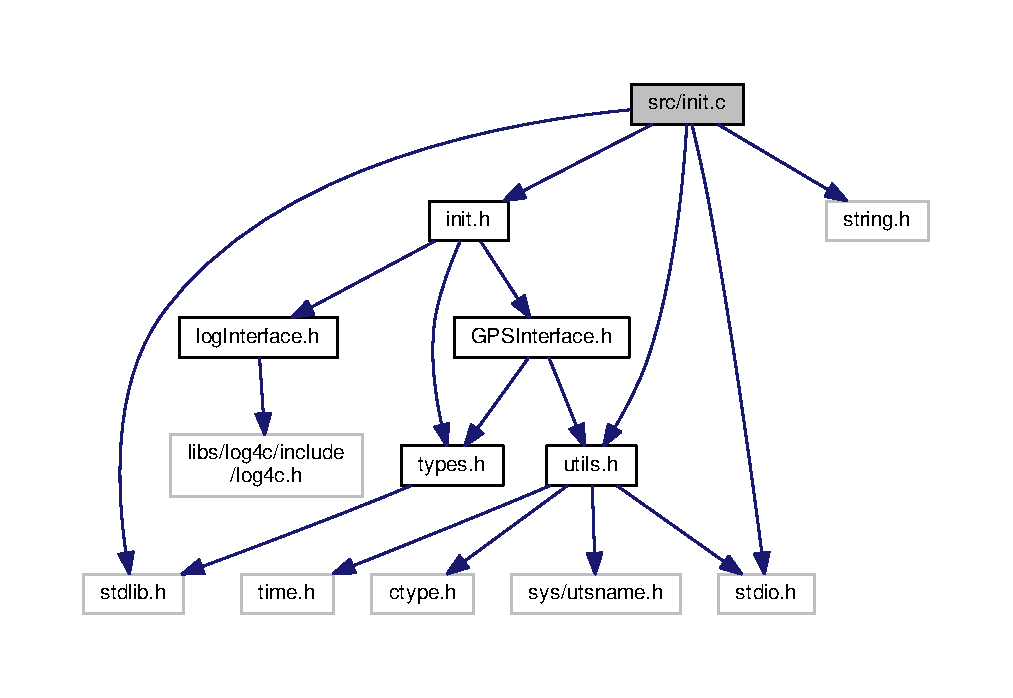
\includegraphics[width=350pt]{init_8c__incl}
\end{center}
\end{figure}
\subsection*{Functions}
\begin{DoxyCompactItemize}
\item 
void \hyperlink{init_8c_a7a5113979d0ecd5e85fc6df200308c1d}{init} (\hyperlink{struct_g_p_s___actions}{G\+P\+S\+\_\+\+Actions} $\ast$G\+P\+S\+Handler, \hyperlink{struct_full_g_p_s_data}{Full\+G\+P\+S\+Data} $\ast$gps\+Data, \hyperlink{struct_zone__general}{Zone\+\_\+general} $\ast$zone, \hyperlink{struct_log___master}{Log\+\_\+\+Master} $\ast$\hyperlink{log_interface_8h_a8970fde3bc8decf8d30eaf4f3c2ce4ed}{log\+Master}, \hyperlink{struct_edge}{Edge} $\ast$$\ast$edges)
\begin{DoxyCompactList}\small\item\em Initialize some important stuff. \end{DoxyCompactList}\item 
int \hyperlink{init_8c_a297ed12bb3b7c61cddbde204b712c786}{parse\+\_\+input\+\_\+args} (\hyperlink{struct_zone__general}{Zone\+\_\+general} $\ast$zone, int argc, char $\ast$$\ast$args)
\begin{DoxyCompactList}\small\item\em Receives argc, argv from main and parses that input. \end{DoxyCompactList}\item 
void \hyperlink{init_8c_a3915bad191609e2ffced09336ee22027}{display\+\_\+help\+\_\+message} (void)
\begin{DoxyCompactList}\small\item\em Display the command-\/line usage statement. \end{DoxyCompactList}\item 
void \hyperlink{init_8c_a81d274388eeddf9b5cddcf4a29af5b0b}{init\+\_\+gps\+\_\+data} (\hyperlink{struct_full_g_p_s_data}{Full\+G\+P\+S\+Data} $\ast$$\ast$gps\+Data)
\begin{DoxyCompactList}\small\item\em initializes the data pointed to by the {\ttfamily struct} pointer \end{DoxyCompactList}\item 
int \hyperlink{init_8c_a0b0b243b7207b2a9f0bb8789c4e9dc6d}{init\+\_\+geofence\+\_\+from\+\_\+argv} (\hyperlink{struct_zone__general}{Zone\+\_\+general} $\ast$zone, int argc, char $\ast$$\ast$args)
\begin{DoxyCompactList}\small\item\em initializes the geofence vertices etc from the argv. the format is xx.\+xxx,xx.\+xxx xx.\+xxx,xx.\+xxx ... etc \end{DoxyCompactList}\item 
int \hyperlink{init_8c_af33c0fcf492f7f9401681bb3be490423}{init\+\_\+geofence\+\_\+from\+\_\+file} (\hyperlink{struct_zone__general}{Zone\+\_\+general} $\ast$zone, char $\ast$$\ast$args)
\begin{DoxyCompactList}\small\item\em initializes the geofence vertices from the data that\textquotesingle{}s user-\/made file which is specified in argv \end{DoxyCompactList}\item 
\hyperlink{struct_g_e_o___point}{G\+E\+O\+\_\+\+Point} \hyperlink{init_8c_a650f4dc11814bda87d60c84827874090}{parse\+\_\+line} (char $\ast$str)
\begin{DoxyCompactList}\small\item\em Parses a single line that contains vertex coordinates. \end{DoxyCompactList}\end{DoxyCompactItemize}


\subsection{Function Documentation}
\index{init.\+c@{init.\+c}!display\+\_\+help\+\_\+message@{display\+\_\+help\+\_\+message}}
\index{display\+\_\+help\+\_\+message@{display\+\_\+help\+\_\+message}!init.\+c@{init.\+c}}
\subsubsection[{\texorpdfstring{display\+\_\+help\+\_\+message(void)}{display_help_message(void)}}]{\setlength{\rightskip}{0pt plus 5cm}void display\+\_\+help\+\_\+message (
\begin{DoxyParamCaption}
\item[{void}]{}
\end{DoxyParamCaption}
)}\hypertarget{init_8c_a3915bad191609e2ffced09336ee22027}{}\label{init_8c_a3915bad191609e2ffced09336ee22027}


Display the command-\/line usage statement. 

\index{init.\+c@{init.\+c}!init@{init}}
\index{init@{init}!init.\+c@{init.\+c}}
\subsubsection[{\texorpdfstring{init(\+G\+P\+S\+\_\+\+Actions $\ast$\+G\+P\+S\+Handler, Full\+G\+P\+S\+Data $\ast$gps\+Data, Zone\+\_\+general $\ast$zone, Log\+\_\+\+Master $\ast$log\+Master, Edge $\ast$$\ast$edges)}{init(GPS_Actions *GPSHandler, FullGPSData *gpsData, Zone_general *zone, Log_Master *logMaster, Edge **edges)}}]{\setlength{\rightskip}{0pt plus 5cm}void init (
\begin{DoxyParamCaption}
\item[{{\bf G\+P\+S\+\_\+\+Actions} $\ast$}]{G\+P\+S\+Handler, }
\item[{{\bf Full\+G\+P\+S\+Data} $\ast$}]{gps\+Data, }
\item[{{\bf Zone\+\_\+general} $\ast$}]{zone, }
\item[{{\bf Log\+\_\+\+Master} $\ast$}]{log\+Master, }
\item[{{\bf Edge} $\ast$$\ast$}]{edges}
\end{DoxyParamCaption}
)}\hypertarget{init_8c_a7a5113979d0ecd5e85fc6df200308c1d}{}\label{init_8c_a7a5113979d0ecd5e85fc6df200308c1d}


Initialize some important stuff. 


\begin{DoxyParams}{Parameters}
{\em G\+P\+S\+Handler} & a pointer to a struct with function pointers to gps related functions. \\
\hline
{\em zone} & pointer to \hyperlink{struct_zone__general}{Zone\+\_\+general} strcut \\
\hline
{\em log\+Master} & pointer to \hyperlink{struct_log___master}{Log\+\_\+\+Master} struct \\
\hline
{\em edges} & double pointer to the \hyperlink{struct_edge}{Edge} struct. pointer to the array of edges of the polygon represented by zone. \\
\hline
\end{DoxyParams}
T\+O\+DO\+: Error checking and rv\index{init.\+c@{init.\+c}!init\+\_\+geofence\+\_\+from\+\_\+argv@{init\+\_\+geofence\+\_\+from\+\_\+argv}}
\index{init\+\_\+geofence\+\_\+from\+\_\+argv@{init\+\_\+geofence\+\_\+from\+\_\+argv}!init.\+c@{init.\+c}}
\subsubsection[{\texorpdfstring{init\+\_\+geofence\+\_\+from\+\_\+argv(\+Zone\+\_\+general $\ast$zone, int argc, char $\ast$$\ast$args)}{init_geofence_from_argv(Zone_general *zone, int argc, char **args)}}]{\setlength{\rightskip}{0pt plus 5cm}int init\+\_\+geofence\+\_\+from\+\_\+argv (
\begin{DoxyParamCaption}
\item[{{\bf Zone\+\_\+general} $\ast$}]{zone, }
\item[{int}]{argc, }
\item[{char $\ast$$\ast$}]{args}
\end{DoxyParamCaption}
)}\hypertarget{init_8c_a0b0b243b7207b2a9f0bb8789c4e9dc6d}{}\label{init_8c_a0b0b243b7207b2a9f0bb8789c4e9dc6d}


initializes the geofence vertices etc from the argv. the format is xx.\+xxx,xx.\+xxx xx.\+xxx,xx.\+xxx ... etc 


\begin{DoxyParams}{Parameters}
{\em zone} & pointer to a \hyperlink{struct_zone__general}{Zone\+\_\+general} struct \\
\hline
{\em argc} & argc \\
\hline
{\em args} & argv\\
\hline
\end{DoxyParams}
\begin{DoxyReturn}{Returns}
one of the error/success codes defined in \hyperlink{init_8h}{init.\+h} 
\end{DoxyReturn}
\index{init.\+c@{init.\+c}!init\+\_\+geofence\+\_\+from\+\_\+file@{init\+\_\+geofence\+\_\+from\+\_\+file}}
\index{init\+\_\+geofence\+\_\+from\+\_\+file@{init\+\_\+geofence\+\_\+from\+\_\+file}!init.\+c@{init.\+c}}
\subsubsection[{\texorpdfstring{init\+\_\+geofence\+\_\+from\+\_\+file(\+Zone\+\_\+general $\ast$zone, char $\ast$$\ast$args)}{init_geofence_from_file(Zone_general *zone, char **args)}}]{\setlength{\rightskip}{0pt plus 5cm}int init\+\_\+geofence\+\_\+from\+\_\+file (
\begin{DoxyParamCaption}
\item[{{\bf Zone\+\_\+general} $\ast$}]{zone, }
\item[{char $\ast$$\ast$}]{args}
\end{DoxyParamCaption}
)}\hypertarget{init_8c_af33c0fcf492f7f9401681bb3be490423}{}\label{init_8c_af33c0fcf492f7f9401681bb3be490423}


initializes the geofence vertices from the data that\textquotesingle{}s user-\/made file which is specified in argv 


\begin{DoxyParams}{Parameters}
{\em zone} & pointer to a \hyperlink{struct_zone__general}{Zone\+\_\+general} struct \\
\hline
{\em args} & argv\\
\hline
\end{DoxyParams}
\begin{DoxyReturn}{Returns}
one of the error/success codes defined in \hyperlink{init_8h}{init.\+h} 
\end{DoxyReturn}
T\+O\+DO\+: proper error checking T\+O\+DO\+: throw an error if geofence in file consists of less than 3 polygons. Add support for a circle geofence (essentialy a cylinder cuz height).\index{init.\+c@{init.\+c}!init\+\_\+gps\+\_\+data@{init\+\_\+gps\+\_\+data}}
\index{init\+\_\+gps\+\_\+data@{init\+\_\+gps\+\_\+data}!init.\+c@{init.\+c}}
\subsubsection[{\texorpdfstring{init\+\_\+gps\+\_\+data(\+Full\+G\+P\+S\+Data $\ast$$\ast$gps\+Data)}{init_gps_data(FullGPSData **gpsData)}}]{\setlength{\rightskip}{0pt plus 5cm}void init\+\_\+gps\+\_\+data (
\begin{DoxyParamCaption}
\item[{{\bf Full\+G\+P\+S\+Data} $\ast$$\ast$}]{gps\+Data}
\end{DoxyParamCaption}
)}\hypertarget{init_8c_a81d274388eeddf9b5cddcf4a29af5b0b}{}\label{init_8c_a81d274388eeddf9b5cddcf4a29af5b0b}


initializes the data pointed to by the {\ttfamily struct} pointer 


\begin{DoxyParams}{Parameters}
{\em gps\+Data} & double pointer to the data \\
\hline
\end{DoxyParams}
\index{init.\+c@{init.\+c}!parse\+\_\+input\+\_\+args@{parse\+\_\+input\+\_\+args}}
\index{parse\+\_\+input\+\_\+args@{parse\+\_\+input\+\_\+args}!init.\+c@{init.\+c}}
\subsubsection[{\texorpdfstring{parse\+\_\+input\+\_\+args(\+Zone\+\_\+general $\ast$zone, int argc, char $\ast$$\ast$args)}{parse_input_args(Zone_general *zone, int argc, char **args)}}]{\setlength{\rightskip}{0pt plus 5cm}int parse\+\_\+input\+\_\+args (
\begin{DoxyParamCaption}
\item[{{\bf Zone\+\_\+general} $\ast$}]{zone, }
\item[{int}]{argc, }
\item[{char $\ast$$\ast$}]{args}
\end{DoxyParamCaption}
)}\hypertarget{init_8c_a297ed12bb3b7c61cddbde204b712c786}{}\label{init_8c_a297ed12bb3b7c61cddbde204b712c786}


Receives argc, argv from main and parses that input. 


\begin{DoxyParams}[1]{Parameters}
 & {\em zone} & A struct with the geofence information (polygon, count, etc.) \\
\hline
\mbox{\tt in}  & {\em argc} & argc \\
\hline
 & {\em args} & argv. should contain the name of the file with the inputs. \\
\hline
\end{DoxyParams}
\begin{DoxyReturn}{Returns}
returns different exit codes (defined in \hyperlink{init_8h}{init.\+h}) depending on the situation. 
\end{DoxyReturn}
T\+O\+DO\+: error checking\index{init.\+c@{init.\+c}!parse\+\_\+line@{parse\+\_\+line}}
\index{parse\+\_\+line@{parse\+\_\+line}!init.\+c@{init.\+c}}
\subsubsection[{\texorpdfstring{parse\+\_\+line(char $\ast$str)}{parse_line(char *str)}}]{\setlength{\rightskip}{0pt plus 5cm}{\bf G\+E\+O\+\_\+\+Point} parse\+\_\+line (
\begin{DoxyParamCaption}
\item[{char $\ast$}]{str}
\end{DoxyParamCaption}
)}\hypertarget{init_8c_a650f4dc11814bda87d60c84827874090}{}\label{init_8c_a650f4dc11814bda87d60c84827874090}


Parses a single line that contains vertex coordinates. 


\begin{DoxyParams}{Parameters}
{\em str} & the line of text that is read from the input file \\
\hline
\end{DoxyParams}
\begin{DoxyReturn}{Returns}
returns a struct of the point, initialized with the coordinates from the line. 
\end{DoxyReturn}

\hypertarget{init_8d}{}\section{src/init.d File Reference}
\label{init_8d}\index{src/init.\+d@{src/init.\+d}}

\hypertarget{init_8h}{}\section{src/init.h File Reference}
\label{init_8h}\index{src/init.\+h@{src/init.\+h}}
{\ttfamily \#include \char`\"{}types.\+h\char`\"{}}\\*
{\ttfamily \#include \char`\"{}log\+Interface.\+h\char`\"{}}\\*
{\ttfamily \#include \char`\"{}G\+P\+S\+Interface.\+h\char`\"{}}\\*
Include dependency graph for init.\+h\+:
\nopagebreak
\begin{figure}[H]
\begin{center}
\leavevmode
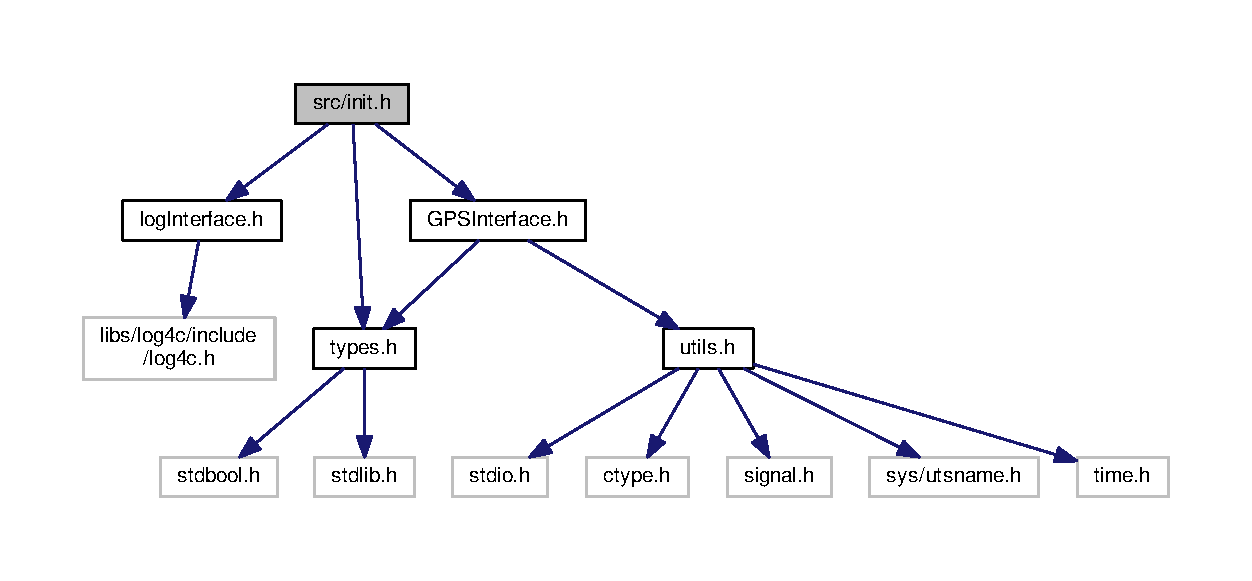
\includegraphics[width=350pt]{init_8h__incl}
\end{center}
\end{figure}
This graph shows which files directly or indirectly include this file\+:\nopagebreak
\begin{figure}[H]
\begin{center}
\leavevmode
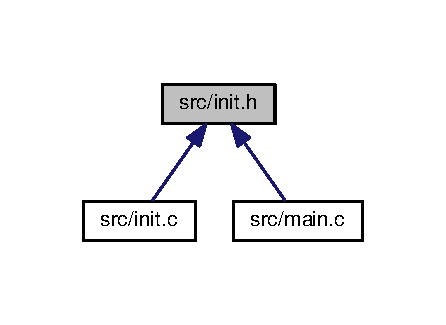
\includegraphics[width=214pt]{init_8h__dep__incl}
\end{center}
\end{figure}
\subsection*{Macros}
\begin{DoxyCompactItemize}
\item 
\#define \hyperlink{init_8h_ac7ef7e3f980b6e01955a54025c3b94df}{C\+O\+M\+M\+O\+N\+\_\+\+E\+R\+R\+\_\+\+S\+TR}~\char`\"{}Try geofence -\/h for help.\textbackslash{}n\char`\"{}
\item 
\#define \hyperlink{init_8h_aa8221631dbe4812db94ed9a6ace57c41}{A\+R\+G\+V\+\_\+\+E\+R\+R\+OR}~1
\item 
\#define \hyperlink{init_8h_aa74d57bc380ee8c7875de73d471c9440}{F\+O\+P\+E\+N\+\_\+\+F\+A\+IL}~2
\item 
\#define \hyperlink{init_8h_affe49ef15a95c80cf814797aed4c7297}{A\+R\+G\+V\+\_\+\+OK}~0
\end{DoxyCompactItemize}
\subsection*{Functions}
\begin{DoxyCompactItemize}
\item 
void \hyperlink{init_8h_a7a5113979d0ecd5e85fc6df200308c1d}{init} (\hyperlink{struct_g_p_s___actions}{G\+P\+S\+\_\+\+Actions} $\ast$G\+P\+S\+Handler, \hyperlink{struct_full_g_p_s_data}{Full\+G\+P\+S\+Data} $\ast$gps\+Data, \hyperlink{struct_zone__general}{Zone\+\_\+general} $\ast$zone, \hyperlink{struct_log___master}{Log\+\_\+\+Master} $\ast$\hyperlink{log_interface_8h_a8970fde3bc8decf8d30eaf4f3c2ce4ed}{log\+Master}, \hyperlink{struct_edge}{Edge} $\ast$$\ast$edges)
\begin{DoxyCompactList}\small\item\em Initialize some important stuff. \end{DoxyCompactList}\item 
void \hyperlink{init_8h_ac28005534dd7638d20979f2c625c72cd}{init\+\_\+platform\+\_\+specific\+\_\+modules} (void)
\begin{DoxyCompactList}\small\item\em calls function to initialize some stuff that works only on the Raspberry-\/\+Pi e.\+g the Wiring\+Pi library or Pi\+Face-\/cad exists only if \#ifdef W\+I\+R\+I\+N\+G\+PI \end{DoxyCompactList}\item 
void \hyperlink{init_8h_a81d274388eeddf9b5cddcf4a29af5b0b}{init\+\_\+gps\+\_\+data} (\hyperlink{struct_full_g_p_s_data}{Full\+G\+P\+S\+Data} $\ast$$\ast$gps\+Data)
\begin{DoxyCompactList}\small\item\em initializes the data pointed to by the {\ttfamily struct} pointer \end{DoxyCompactList}\item 
int \hyperlink{init_8h_a297ed12bb3b7c61cddbde204b712c786}{parse\+\_\+input\+\_\+args} (\hyperlink{struct_zone__general}{Zone\+\_\+general} $\ast$zone, int argc, char $\ast$$\ast$args)
\begin{DoxyCompactList}\small\item\em Receives argc, argv from main and parses that input. \end{DoxyCompactList}\item 
int \hyperlink{init_8h_a0b0b243b7207b2a9f0bb8789c4e9dc6d}{init\+\_\+geofence\+\_\+from\+\_\+argv} (\hyperlink{struct_zone__general}{Zone\+\_\+general} $\ast$zone, int argc, char $\ast$$\ast$args)
\begin{DoxyCompactList}\small\item\em initializes the geofence vertices etc from the argv. the format is xx.\+xxx,xx.\+xxx xx.\+xxx,xx.\+xxx ... etc \end{DoxyCompactList}\item 
int \hyperlink{init_8h_af33c0fcf492f7f9401681bb3be490423}{init\+\_\+geofence\+\_\+from\+\_\+file} (\hyperlink{struct_zone__general}{Zone\+\_\+general} $\ast$zone, char $\ast$$\ast$args)
\begin{DoxyCompactList}\small\item\em initializes the geofence vertices from the data that\textquotesingle{}s user-\/made file which is specified in argv \end{DoxyCompactList}\item 
void \hyperlink{init_8h_a3915bad191609e2ffced09336ee22027}{display\+\_\+help\+\_\+message} (void)
\begin{DoxyCompactList}\small\item\em Display the command-\/line usage statement. \end{DoxyCompactList}\item 
\hyperlink{struct_g_e_o___point}{G\+E\+O\+\_\+\+Point} \hyperlink{init_8h_a650f4dc11814bda87d60c84827874090}{parse\+\_\+line} (char $\ast$str)
\begin{DoxyCompactList}\small\item\em Parses a single line that contains vertex coordinates. \end{DoxyCompactList}\end{DoxyCompactItemize}
\subsection*{Variables}
\begin{DoxyCompactItemize}
\item 
F\+I\+LE $\ast$ \hyperlink{init_8h_a7a9ef3013c9c75feae52a6c9a8b7eedb}{argv\+Input\+File}
\end{DoxyCompactItemize}


\subsection{Macro Definition Documentation}
\index{init.\+h@{init.\+h}!A\+R\+G\+V\+\_\+\+E\+R\+R\+OR@{A\+R\+G\+V\+\_\+\+E\+R\+R\+OR}}
\index{A\+R\+G\+V\+\_\+\+E\+R\+R\+OR@{A\+R\+G\+V\+\_\+\+E\+R\+R\+OR}!init.\+h@{init.\+h}}
\subsubsection[{\texorpdfstring{A\+R\+G\+V\+\_\+\+E\+R\+R\+OR}{ARGV_ERROR}}]{\setlength{\rightskip}{0pt plus 5cm}\#define A\+R\+G\+V\+\_\+\+E\+R\+R\+OR~1}\hypertarget{init_8h_aa8221631dbe4812db94ed9a6ace57c41}{}\label{init_8h_aa8221631dbe4812db94ed9a6ace57c41}
\index{init.\+h@{init.\+h}!A\+R\+G\+V\+\_\+\+OK@{A\+R\+G\+V\+\_\+\+OK}}
\index{A\+R\+G\+V\+\_\+\+OK@{A\+R\+G\+V\+\_\+\+OK}!init.\+h@{init.\+h}}
\subsubsection[{\texorpdfstring{A\+R\+G\+V\+\_\+\+OK}{ARGV_OK}}]{\setlength{\rightskip}{0pt plus 5cm}\#define A\+R\+G\+V\+\_\+\+OK~0}\hypertarget{init_8h_affe49ef15a95c80cf814797aed4c7297}{}\label{init_8h_affe49ef15a95c80cf814797aed4c7297}
\index{init.\+h@{init.\+h}!C\+O\+M\+M\+O\+N\+\_\+\+E\+R\+R\+\_\+\+S\+TR@{C\+O\+M\+M\+O\+N\+\_\+\+E\+R\+R\+\_\+\+S\+TR}}
\index{C\+O\+M\+M\+O\+N\+\_\+\+E\+R\+R\+\_\+\+S\+TR@{C\+O\+M\+M\+O\+N\+\_\+\+E\+R\+R\+\_\+\+S\+TR}!init.\+h@{init.\+h}}
\subsubsection[{\texorpdfstring{C\+O\+M\+M\+O\+N\+\_\+\+E\+R\+R\+\_\+\+S\+TR}{COMMON_ERR_STR}}]{\setlength{\rightskip}{0pt plus 5cm}\#define C\+O\+M\+M\+O\+N\+\_\+\+E\+R\+R\+\_\+\+S\+TR~\char`\"{}Try geofence -\/h for help.\textbackslash{}n\char`\"{}}\hypertarget{init_8h_ac7ef7e3f980b6e01955a54025c3b94df}{}\label{init_8h_ac7ef7e3f980b6e01955a54025c3b94df}
\index{init.\+h@{init.\+h}!F\+O\+P\+E\+N\+\_\+\+F\+A\+IL@{F\+O\+P\+E\+N\+\_\+\+F\+A\+IL}}
\index{F\+O\+P\+E\+N\+\_\+\+F\+A\+IL@{F\+O\+P\+E\+N\+\_\+\+F\+A\+IL}!init.\+h@{init.\+h}}
\subsubsection[{\texorpdfstring{F\+O\+P\+E\+N\+\_\+\+F\+A\+IL}{FOPEN_FAIL}}]{\setlength{\rightskip}{0pt plus 5cm}\#define F\+O\+P\+E\+N\+\_\+\+F\+A\+IL~2}\hypertarget{init_8h_aa74d57bc380ee8c7875de73d471c9440}{}\label{init_8h_aa74d57bc380ee8c7875de73d471c9440}


\subsection{Function Documentation}
\index{init.\+h@{init.\+h}!display\+\_\+help\+\_\+message@{display\+\_\+help\+\_\+message}}
\index{display\+\_\+help\+\_\+message@{display\+\_\+help\+\_\+message}!init.\+h@{init.\+h}}
\subsubsection[{\texorpdfstring{display\+\_\+help\+\_\+message(void)}{display_help_message(void)}}]{\setlength{\rightskip}{0pt plus 5cm}void display\+\_\+help\+\_\+message (
\begin{DoxyParamCaption}
\item[{void}]{}
\end{DoxyParamCaption}
)}\hypertarget{init_8h_a3915bad191609e2ffced09336ee22027}{}\label{init_8h_a3915bad191609e2ffced09336ee22027}


Display the command-\/line usage statement. 

\index{init.\+h@{init.\+h}!init@{init}}
\index{init@{init}!init.\+h@{init.\+h}}
\subsubsection[{\texorpdfstring{init(\+G\+P\+S\+\_\+\+Actions $\ast$\+G\+P\+S\+Handler, Full\+G\+P\+S\+Data $\ast$gps\+Data, Zone\+\_\+general $\ast$zone, Log\+\_\+\+Master $\ast$log\+Master, Edge $\ast$$\ast$edges)}{init(GPS_Actions *GPSHandler, FullGPSData *gpsData, Zone_general *zone, Log_Master *logMaster, Edge **edges)}}]{\setlength{\rightskip}{0pt plus 5cm}void init (
\begin{DoxyParamCaption}
\item[{{\bf G\+P\+S\+\_\+\+Actions} $\ast$}]{G\+P\+S\+Handler, }
\item[{{\bf Full\+G\+P\+S\+Data} $\ast$}]{gps\+Data, }
\item[{{\bf Zone\+\_\+general} $\ast$}]{zone, }
\item[{{\bf Log\+\_\+\+Master} $\ast$}]{log\+Master, }
\item[{{\bf Edge} $\ast$$\ast$}]{edges}
\end{DoxyParamCaption}
)}\hypertarget{init_8h_a7a5113979d0ecd5e85fc6df200308c1d}{}\label{init_8h_a7a5113979d0ecd5e85fc6df200308c1d}


Initialize some important stuff. 


\begin{DoxyParams}{Parameters}
{\em G\+P\+S\+Handler} & a pointer to a struct with function pointers to gps related functions. \\
\hline
{\em zone} & pointer to \hyperlink{struct_zone__general}{Zone\+\_\+general} strcut \\
\hline
{\em log\+Master} & pointer to \hyperlink{struct_log___master}{Log\+\_\+\+Master} struct \\
\hline
{\em edges} & double pointer to the \hyperlink{struct_edge}{Edge} struct. pointer to the array of edges of the polygon represented by zone. \\
\hline
\end{DoxyParams}
T\+O\+DO\+: Error checking and rv\index{init.\+h@{init.\+h}!init\+\_\+geofence\+\_\+from\+\_\+argv@{init\+\_\+geofence\+\_\+from\+\_\+argv}}
\index{init\+\_\+geofence\+\_\+from\+\_\+argv@{init\+\_\+geofence\+\_\+from\+\_\+argv}!init.\+h@{init.\+h}}
\subsubsection[{\texorpdfstring{init\+\_\+geofence\+\_\+from\+\_\+argv(\+Zone\+\_\+general $\ast$zone, int argc, char $\ast$$\ast$args)}{init_geofence_from_argv(Zone_general *zone, int argc, char **args)}}]{\setlength{\rightskip}{0pt plus 5cm}int init\+\_\+geofence\+\_\+from\+\_\+argv (
\begin{DoxyParamCaption}
\item[{{\bf Zone\+\_\+general} $\ast$}]{zone, }
\item[{int}]{argc, }
\item[{char $\ast$$\ast$}]{args}
\end{DoxyParamCaption}
)}\hypertarget{init_8h_a0b0b243b7207b2a9f0bb8789c4e9dc6d}{}\label{init_8h_a0b0b243b7207b2a9f0bb8789c4e9dc6d}


initializes the geofence vertices etc from the argv. the format is xx.\+xxx,xx.\+xxx xx.\+xxx,xx.\+xxx ... etc 


\begin{DoxyParams}{Parameters}
{\em zone} & pointer to a \hyperlink{struct_zone__general}{Zone\+\_\+general} struct \\
\hline
{\em argc} & argc \\
\hline
{\em args} & argv\\
\hline
\end{DoxyParams}
\begin{DoxyReturn}{Returns}
one of the error/success codes defined in \hyperlink{init_8h}{init.\+h} 
\end{DoxyReturn}
\index{init.\+h@{init.\+h}!init\+\_\+geofence\+\_\+from\+\_\+file@{init\+\_\+geofence\+\_\+from\+\_\+file}}
\index{init\+\_\+geofence\+\_\+from\+\_\+file@{init\+\_\+geofence\+\_\+from\+\_\+file}!init.\+h@{init.\+h}}
\subsubsection[{\texorpdfstring{init\+\_\+geofence\+\_\+from\+\_\+file(\+Zone\+\_\+general $\ast$zone, char $\ast$$\ast$args)}{init_geofence_from_file(Zone_general *zone, char **args)}}]{\setlength{\rightskip}{0pt plus 5cm}int init\+\_\+geofence\+\_\+from\+\_\+file (
\begin{DoxyParamCaption}
\item[{{\bf Zone\+\_\+general} $\ast$}]{zone, }
\item[{char $\ast$$\ast$}]{args}
\end{DoxyParamCaption}
)}\hypertarget{init_8h_af33c0fcf492f7f9401681bb3be490423}{}\label{init_8h_af33c0fcf492f7f9401681bb3be490423}


initializes the geofence vertices from the data that\textquotesingle{}s user-\/made file which is specified in argv 


\begin{DoxyParams}{Parameters}
{\em zone} & pointer to a \hyperlink{struct_zone__general}{Zone\+\_\+general} struct \\
\hline
{\em args} & argv\\
\hline
\end{DoxyParams}
\begin{DoxyReturn}{Returns}
one of the error/success codes defined in \hyperlink{init_8h}{init.\+h} 
\end{DoxyReturn}
T\+O\+DO\+: proper error checking T\+O\+DO\+: throw an error if geofence in file consists of less than 3 polygons. Add support for a circle geofence (essentialy a cylinder cuz height).\index{init.\+h@{init.\+h}!init\+\_\+gps\+\_\+data@{init\+\_\+gps\+\_\+data}}
\index{init\+\_\+gps\+\_\+data@{init\+\_\+gps\+\_\+data}!init.\+h@{init.\+h}}
\subsubsection[{\texorpdfstring{init\+\_\+gps\+\_\+data(\+Full\+G\+P\+S\+Data $\ast$$\ast$gps\+Data)}{init_gps_data(FullGPSData **gpsData)}}]{\setlength{\rightskip}{0pt plus 5cm}void init\+\_\+gps\+\_\+data (
\begin{DoxyParamCaption}
\item[{{\bf Full\+G\+P\+S\+Data} $\ast$$\ast$}]{gps\+Data}
\end{DoxyParamCaption}
)}\hypertarget{init_8h_a81d274388eeddf9b5cddcf4a29af5b0b}{}\label{init_8h_a81d274388eeddf9b5cddcf4a29af5b0b}


initializes the data pointed to by the {\ttfamily struct} pointer 


\begin{DoxyParams}{Parameters}
{\em gps\+Data} & double pointer to the data \\
\hline
\end{DoxyParams}
\index{init.\+h@{init.\+h}!init\+\_\+platform\+\_\+specific\+\_\+modules@{init\+\_\+platform\+\_\+specific\+\_\+modules}}
\index{init\+\_\+platform\+\_\+specific\+\_\+modules@{init\+\_\+platform\+\_\+specific\+\_\+modules}!init.\+h@{init.\+h}}
\subsubsection[{\texorpdfstring{init\+\_\+platform\+\_\+specific\+\_\+modules(void)}{init_platform_specific_modules(void)}}]{\setlength{\rightskip}{0pt plus 5cm}void init\+\_\+platform\+\_\+specific\+\_\+modules (
\begin{DoxyParamCaption}
\item[{void}]{}
\end{DoxyParamCaption}
)}\hypertarget{init_8h_ac28005534dd7638d20979f2c625c72cd}{}\label{init_8h_ac28005534dd7638d20979f2c625c72cd}


calls function to initialize some stuff that works only on the Raspberry-\/\+Pi e.\+g the Wiring\+Pi library or Pi\+Face-\/cad exists only if \#ifdef W\+I\+R\+I\+N\+G\+PI 

\index{init.\+h@{init.\+h}!parse\+\_\+input\+\_\+args@{parse\+\_\+input\+\_\+args}}
\index{parse\+\_\+input\+\_\+args@{parse\+\_\+input\+\_\+args}!init.\+h@{init.\+h}}
\subsubsection[{\texorpdfstring{parse\+\_\+input\+\_\+args(\+Zone\+\_\+general $\ast$zone, int argc, char $\ast$$\ast$args)}{parse_input_args(Zone_general *zone, int argc, char **args)}}]{\setlength{\rightskip}{0pt plus 5cm}int parse\+\_\+input\+\_\+args (
\begin{DoxyParamCaption}
\item[{{\bf Zone\+\_\+general} $\ast$}]{zone, }
\item[{int}]{argc, }
\item[{char $\ast$$\ast$}]{args}
\end{DoxyParamCaption}
)}\hypertarget{init_8h_a297ed12bb3b7c61cddbde204b712c786}{}\label{init_8h_a297ed12bb3b7c61cddbde204b712c786}


Receives argc, argv from main and parses that input. 


\begin{DoxyParams}[1]{Parameters}
 & {\em zone} & A struct with the geofence information (polygon, count, etc.) \\
\hline
\mbox{\tt in}  & {\em argc} & argc \\
\hline
 & {\em args} & argv. should contain the name of the file with the inputs. \\
\hline
\end{DoxyParams}
\begin{DoxyReturn}{Returns}
returns different exit codes (defined in \hyperlink{init_8h}{init.\+h}) depending on the situation. 
\end{DoxyReturn}
T\+O\+DO\+: error checking\index{init.\+h@{init.\+h}!parse\+\_\+line@{parse\+\_\+line}}
\index{parse\+\_\+line@{parse\+\_\+line}!init.\+h@{init.\+h}}
\subsubsection[{\texorpdfstring{parse\+\_\+line(char $\ast$str)}{parse_line(char *str)}}]{\setlength{\rightskip}{0pt plus 5cm}{\bf G\+E\+O\+\_\+\+Point} parse\+\_\+line (
\begin{DoxyParamCaption}
\item[{char $\ast$}]{str}
\end{DoxyParamCaption}
)}\hypertarget{init_8h_a650f4dc11814bda87d60c84827874090}{}\label{init_8h_a650f4dc11814bda87d60c84827874090}


Parses a single line that contains vertex coordinates. 


\begin{DoxyParams}{Parameters}
{\em str} & the line of text that is read from the input file \\
\hline
\end{DoxyParams}
\begin{DoxyReturn}{Returns}
returns a struct of the point, initialized with the coordinates from the line. 
\end{DoxyReturn}


\subsection{Variable Documentation}
\index{init.\+h@{init.\+h}!argv\+Input\+File@{argv\+Input\+File}}
\index{argv\+Input\+File@{argv\+Input\+File}!init.\+h@{init.\+h}}
\subsubsection[{\texorpdfstring{argv\+Input\+File}{argvInputFile}}]{\setlength{\rightskip}{0pt plus 5cm}F\+I\+LE$\ast$ argv\+Input\+File}\hypertarget{init_8h_a7a9ef3013c9c75feae52a6c9a8b7eedb}{}\label{init_8h_a7a9ef3013c9c75feae52a6c9a8b7eedb}

\hypertarget{log_interface_8c}{}\section{src/log\+Interface.c File Reference}
\label{log_interface_8c}\index{src/log\+Interface.\+c@{src/log\+Interface.\+c}}
{\ttfamily \#include \char`\"{}log\+Interface.\+h\char`\"{}}\\*
Include dependency graph for log\+Interface.\+c\+:
\nopagebreak
\begin{figure}[H]
\begin{center}
\leavevmode
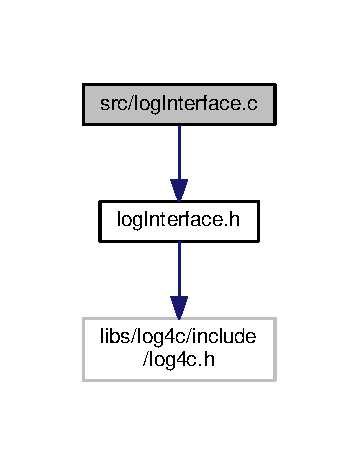
\includegraphics[width=172pt]{log_interface_8c__incl}
\end{center}
\end{figure}
\subsection*{Functions}
\begin{DoxyCompactItemize}
\item 
int \hyperlink{log_interface_8c_a00bc922ef3d55d2d8b5f9457c1dcc0b1}{init\+Log\+System} (\hyperlink{struct_log___master}{Log\+\_\+\+Master} $\ast$\hyperlink{log_interface_8h_a8970fde3bc8decf8d30eaf4f3c2ce4ed}{log\+Master})
\begin{DoxyCompactList}\small\item\em initializes the Loggers from log4c library \end{DoxyCompactList}\item 
void \hyperlink{log_interface_8c_a36b40dbd7b238cda6c595cf4c364ee3b}{log\+Event} (char $\ast$str, int priority, int log\+Type, \hyperlink{struct_log___master}{Log\+\_\+\+Master} $\ast$\hyperlink{log_interface_8h_a8970fde3bc8decf8d30eaf4f3c2ce4ed}{log\+Master})
\begin{DoxyCompactList}\small\item\em logs the message into the specified stream, using the specifeied logger. \end{DoxyCompactList}\item 
int \hyperlink{log_interface_8c_a76fb3b7c139c9d2ec85c565cc48e4b7a}{fini\+Log\+System} (void)
\begin{DoxyCompactList}\small\item\em close and stop the logging system \end{DoxyCompactList}\end{DoxyCompactItemize}


\subsection{Function Documentation}
\index{log\+Interface.\+c@{log\+Interface.\+c}!fini\+Log\+System@{fini\+Log\+System}}
\index{fini\+Log\+System@{fini\+Log\+System}!log\+Interface.\+c@{log\+Interface.\+c}}
\subsubsection[{\texorpdfstring{fini\+Log\+System(void)}{finiLogSystem(void)}}]{\setlength{\rightskip}{0pt plus 5cm}int fini\+Log\+System (
\begin{DoxyParamCaption}
\item[{void}]{}
\end{DoxyParamCaption}
)}\hypertarget{log_interface_8c_a76fb3b7c139c9d2ec85c565cc48e4b7a}{}\label{log_interface_8c_a76fb3b7c139c9d2ec85c565cc48e4b7a}


close and stop the logging system 

\begin{DoxyReturn}{Returns}
err\+Code 
\end{DoxyReturn}
\index{log\+Interface.\+c@{log\+Interface.\+c}!init\+Log\+System@{init\+Log\+System}}
\index{init\+Log\+System@{init\+Log\+System}!log\+Interface.\+c@{log\+Interface.\+c}}
\subsubsection[{\texorpdfstring{init\+Log\+System(\+Log\+\_\+\+Master $\ast$log\+Master)}{initLogSystem(Log_Master *logMaster)}}]{\setlength{\rightskip}{0pt plus 5cm}int init\+Log\+System (
\begin{DoxyParamCaption}
\item[{{\bf Log\+\_\+\+Master} $\ast$}]{log\+Master}
\end{DoxyParamCaption}
)}\hypertarget{log_interface_8c_a00bc922ef3d55d2d8b5f9457c1dcc0b1}{}\label{log_interface_8c_a00bc922ef3d55d2d8b5f9457c1dcc0b1}


initializes the Loggers from log4c library 


\begin{DoxyParams}{Parameters}
{\em log\+Master} & Log\+Master struct that contains all loggers \\
\hline
\end{DoxyParams}
\begin{DoxyReturn}{Returns}
err\+Code 
\end{DoxyReturn}
F\+I\+X\+ME\+: if the log\+Instance\+Name attribute of the \hyperlink{struct_logger}{Logger} struct, is set to \char`\"{}\char`\"{} in all of the loggers, they stop working and only one logger works with only one log stream (be it E\+R\+R\+OR, N\+M\+EA or I\+N\+FO). find a way to get rid of this string A\+ND keep the logs on.\index{log\+Interface.\+c@{log\+Interface.\+c}!log\+Event@{log\+Event}}
\index{log\+Event@{log\+Event}!log\+Interface.\+c@{log\+Interface.\+c}}
\subsubsection[{\texorpdfstring{log\+Event(char $\ast$str, int priority, int log\+Type, Log\+\_\+\+Master $\ast$log\+Master)}{logEvent(char *str, int priority, int logType, Log_Master *logMaster)}}]{\setlength{\rightskip}{0pt plus 5cm}void log\+Event (
\begin{DoxyParamCaption}
\item[{char $\ast$}]{str, }
\item[{int}]{priority, }
\item[{int}]{log\+Type, }
\item[{{\bf Log\+\_\+\+Master} $\ast$}]{log\+Master}
\end{DoxyParamCaption}
)}\hypertarget{log_interface_8c_a36b40dbd7b238cda6c595cf4c364ee3b}{}\label{log_interface_8c_a36b40dbd7b238cda6c595cf4c364ee3b}


logs the message into the specified stream, using the specifeied logger. 


\begin{DoxyParams}[1]{Parameters}
 & {\em str} & the log message \\
\hline
\mbox{\tt in}  & {\em priority} & priority of the log. see L\+O\+G4\+C\+\_\+\+P\+R\+I\+O\+R\+I\+TY enums. (log4c\+\_\+priority\+\_\+level\+\_\+t) \\
\hline
\mbox{\tt in}  & {\em log\+Type} & The log type \\
\hline
 & {\em log\+Master} & a pointer to the \hyperlink{struct_log___master}{Log\+\_\+\+Master} struct that contains log objects \\
\hline
\end{DoxyParams}

\hypertarget{log_interface_8d}{}\section{src/log\+Interface.d File Reference}
\label{log_interface_8d}\index{src/log\+Interface.\+d@{src/log\+Interface.\+d}}

\hypertarget{log_interface_8h}{}\section{src/log\+Interface.h File Reference}
\label{log_interface_8h}\index{src/log\+Interface.\+h@{src/log\+Interface.\+h}}
{\ttfamily \#include $<$libs/log4c/include/log4c.\+h$>$}\\*
Include dependency graph for log\+Interface.\+h\+:\nopagebreak
\begin{figure}[H]
\begin{center}
\leavevmode
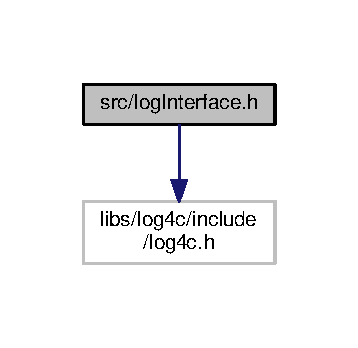
\includegraphics[width=172pt]{log_interface_8h__incl}
\end{center}
\end{figure}
This graph shows which files directly or indirectly include this file\+:\nopagebreak
\begin{figure}[H]
\begin{center}
\leavevmode
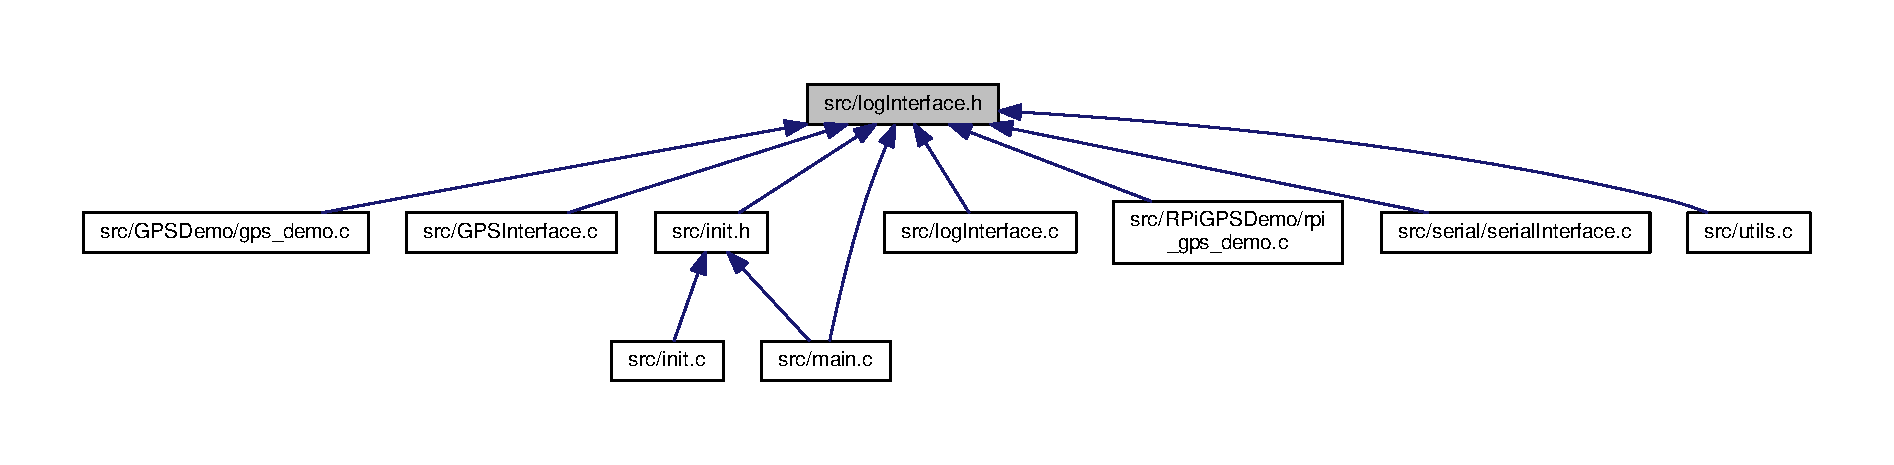
\includegraphics[width=350pt]{log_interface_8h__dep__incl}
\end{center}
\end{figure}
\subsection*{Data Structures}
\begin{DoxyCompactItemize}
\item 
struct \hyperlink{struct_logger}{Logger}
\begin{DoxyCompactList}\small\item\em Represents a single type of logger (e.\+g. one for error, one for info, etc.) \end{DoxyCompactList}\item 
struct \hyperlink{struct_log___master}{Log\+\_\+\+Master}
\begin{DoxyCompactList}\small\item\em Holds all the loggers that are used to record different types of logs. \end{DoxyCompactList}\end{DoxyCompactItemize}
\subsection*{Macros}
\begin{DoxyCompactItemize}
\item 
\#define \hyperlink{log_interface_8h_a2828adfcf264106c20bc76360f2d139e}{O\+P\+E\+R\+A\+T\+I\+O\+N\+\_\+\+L\+O\+G\+\_\+\+F\+I\+LE}~\char`\"{}logs/operation.\+log\char`\"{}
\item 
\#define \hyperlink{log_interface_8h_a4d587ea1f7578d4e3a120b9dd6c7e5bc}{N\+M\+E\+A\+\_\+\+L\+O\+G\+\_\+\+F\+I\+LE}~\char`\"{}logs/nmea.\+log\char`\"{}
\item 
\#define \hyperlink{log_interface_8h_a96cb1a428d93baa38aa5c77b4fe19766}{E\+R\+R\+O\+R\+\_\+\+L\+O\+G\+\_\+\+F\+I\+LE}~\char`\"{}logs/errors.\+log\char`\"{}
\item 
\#define \hyperlink{log_interface_8h_ae1103fea1e1b3c41ca3322d5389f7162}{I\+N\+FO}~0
\item 
\#define \hyperlink{log_interface_8h_a8fe83ac76edc595f6b98cd4a4127aed5}{E\+R\+R\+OR}~1
\item 
\#define \hyperlink{log_interface_8h_aa713da6fe25220d5fbd264a0568afa42}{N\+M\+EA}~2
\end{DoxyCompactItemize}
\subsection*{Typedefs}
\begin{DoxyCompactItemize}
\item 
typedef struct \hyperlink{struct_logger}{Logger} \hyperlink{log_interface_8h_a44e00dcfd51205e4319f61c3338316c2}{Logger}
\begin{DoxyCompactList}\small\item\em Represents a single type of logger (e.\+g. one for error, one for info, etc.) \end{DoxyCompactList}\item 
typedef struct \hyperlink{struct_log___master}{Log\+\_\+\+Master} \hyperlink{log_interface_8h_a1b940cbb9f51692afabbb43cff7446ce}{Log\+\_\+\+Master}
\begin{DoxyCompactList}\small\item\em Holds all the loggers that are used to record different types of logs. \end{DoxyCompactList}\end{DoxyCompactItemize}
\subsection*{Functions}
\begin{DoxyCompactItemize}
\item 
int \hyperlink{log_interface_8h_a00bc922ef3d55d2d8b5f9457c1dcc0b1}{init\+Log\+System} (\hyperlink{struct_log___master}{Log\+\_\+\+Master} $\ast$\hyperlink{log_interface_8h_a8970fde3bc8decf8d30eaf4f3c2ce4ed}{log\+Master})
\begin{DoxyCompactList}\small\item\em initializes the Loggers from log4c library \end{DoxyCompactList}\item 
int \hyperlink{log_interface_8h_a76fb3b7c139c9d2ec85c565cc48e4b7a}{fini\+Log\+System} (void)
\begin{DoxyCompactList}\small\item\em close and stop the logging system \end{DoxyCompactList}\item 
void \hyperlink{log_interface_8h_a36b40dbd7b238cda6c595cf4c364ee3b}{log\+Event} (char $\ast$str, int priority, int log\+Type, \hyperlink{struct_log___master}{Log\+\_\+\+Master} $\ast$\hyperlink{log_interface_8h_a8970fde3bc8decf8d30eaf4f3c2ce4ed}{log\+Master})
\begin{DoxyCompactList}\small\item\em logs the message into the specified stream, using the specified logger. \end{DoxyCompactList}\end{DoxyCompactItemize}
\subsection*{Variables}
\begin{DoxyCompactItemize}
\item 
\hyperlink{struct_log___master}{Log\+\_\+\+Master} \hyperlink{log_interface_8h_a8970fde3bc8decf8d30eaf4f3c2ce4ed}{log\+Master}
\end{DoxyCompactItemize}


\subsection{Macro Definition Documentation}
\index{log\+Interface.\+h@{log\+Interface.\+h}!E\+R\+R\+OR@{E\+R\+R\+OR}}
\index{E\+R\+R\+OR@{E\+R\+R\+OR}!log\+Interface.\+h@{log\+Interface.\+h}}
\subsubsection[{\texorpdfstring{E\+R\+R\+OR}{ERROR}}]{\setlength{\rightskip}{0pt plus 5cm}\#define E\+R\+R\+OR~1}\hypertarget{log_interface_8h_a8fe83ac76edc595f6b98cd4a4127aed5}{}\label{log_interface_8h_a8fe83ac76edc595f6b98cd4a4127aed5}
\index{log\+Interface.\+h@{log\+Interface.\+h}!E\+R\+R\+O\+R\+\_\+\+L\+O\+G\+\_\+\+F\+I\+LE@{E\+R\+R\+O\+R\+\_\+\+L\+O\+G\+\_\+\+F\+I\+LE}}
\index{E\+R\+R\+O\+R\+\_\+\+L\+O\+G\+\_\+\+F\+I\+LE@{E\+R\+R\+O\+R\+\_\+\+L\+O\+G\+\_\+\+F\+I\+LE}!log\+Interface.\+h@{log\+Interface.\+h}}
\subsubsection[{\texorpdfstring{E\+R\+R\+O\+R\+\_\+\+L\+O\+G\+\_\+\+F\+I\+LE}{ERROR_LOG_FILE}}]{\setlength{\rightskip}{0pt plus 5cm}\#define E\+R\+R\+O\+R\+\_\+\+L\+O\+G\+\_\+\+F\+I\+LE~\char`\"{}logs/errors.\+log\char`\"{}}\hypertarget{log_interface_8h_a96cb1a428d93baa38aa5c77b4fe19766}{}\label{log_interface_8h_a96cb1a428d93baa38aa5c77b4fe19766}
\index{log\+Interface.\+h@{log\+Interface.\+h}!I\+N\+FO@{I\+N\+FO}}
\index{I\+N\+FO@{I\+N\+FO}!log\+Interface.\+h@{log\+Interface.\+h}}
\subsubsection[{\texorpdfstring{I\+N\+FO}{INFO}}]{\setlength{\rightskip}{0pt plus 5cm}\#define I\+N\+FO~0}\hypertarget{log_interface_8h_ae1103fea1e1b3c41ca3322d5389f7162}{}\label{log_interface_8h_ae1103fea1e1b3c41ca3322d5389f7162}
\index{log\+Interface.\+h@{log\+Interface.\+h}!N\+M\+EA@{N\+M\+EA}}
\index{N\+M\+EA@{N\+M\+EA}!log\+Interface.\+h@{log\+Interface.\+h}}
\subsubsection[{\texorpdfstring{N\+M\+EA}{NMEA}}]{\setlength{\rightskip}{0pt plus 5cm}\#define N\+M\+EA~2}\hypertarget{log_interface_8h_aa713da6fe25220d5fbd264a0568afa42}{}\label{log_interface_8h_aa713da6fe25220d5fbd264a0568afa42}
\index{log\+Interface.\+h@{log\+Interface.\+h}!N\+M\+E\+A\+\_\+\+L\+O\+G\+\_\+\+F\+I\+LE@{N\+M\+E\+A\+\_\+\+L\+O\+G\+\_\+\+F\+I\+LE}}
\index{N\+M\+E\+A\+\_\+\+L\+O\+G\+\_\+\+F\+I\+LE@{N\+M\+E\+A\+\_\+\+L\+O\+G\+\_\+\+F\+I\+LE}!log\+Interface.\+h@{log\+Interface.\+h}}
\subsubsection[{\texorpdfstring{N\+M\+E\+A\+\_\+\+L\+O\+G\+\_\+\+F\+I\+LE}{NMEA_LOG_FILE}}]{\setlength{\rightskip}{0pt plus 5cm}\#define N\+M\+E\+A\+\_\+\+L\+O\+G\+\_\+\+F\+I\+LE~\char`\"{}logs/nmea.\+log\char`\"{}}\hypertarget{log_interface_8h_a4d587ea1f7578d4e3a120b9dd6c7e5bc}{}\label{log_interface_8h_a4d587ea1f7578d4e3a120b9dd6c7e5bc}
\index{log\+Interface.\+h@{log\+Interface.\+h}!O\+P\+E\+R\+A\+T\+I\+O\+N\+\_\+\+L\+O\+G\+\_\+\+F\+I\+LE@{O\+P\+E\+R\+A\+T\+I\+O\+N\+\_\+\+L\+O\+G\+\_\+\+F\+I\+LE}}
\index{O\+P\+E\+R\+A\+T\+I\+O\+N\+\_\+\+L\+O\+G\+\_\+\+F\+I\+LE@{O\+P\+E\+R\+A\+T\+I\+O\+N\+\_\+\+L\+O\+G\+\_\+\+F\+I\+LE}!log\+Interface.\+h@{log\+Interface.\+h}}
\subsubsection[{\texorpdfstring{O\+P\+E\+R\+A\+T\+I\+O\+N\+\_\+\+L\+O\+G\+\_\+\+F\+I\+LE}{OPERATION_LOG_FILE}}]{\setlength{\rightskip}{0pt plus 5cm}\#define O\+P\+E\+R\+A\+T\+I\+O\+N\+\_\+\+L\+O\+G\+\_\+\+F\+I\+LE~\char`\"{}logs/operation.\+log\char`\"{}}\hypertarget{log_interface_8h_a2828adfcf264106c20bc76360f2d139e}{}\label{log_interface_8h_a2828adfcf264106c20bc76360f2d139e}


\subsection{Typedef Documentation}
\index{log\+Interface.\+h@{log\+Interface.\+h}!Log\+\_\+\+Master@{Log\+\_\+\+Master}}
\index{Log\+\_\+\+Master@{Log\+\_\+\+Master}!log\+Interface.\+h@{log\+Interface.\+h}}
\subsubsection[{\texorpdfstring{Log\+\_\+\+Master}{Log_Master}}]{\setlength{\rightskip}{0pt plus 5cm}typedef struct {\bf Log\+\_\+\+Master}  {\bf Log\+\_\+\+Master}}\hypertarget{log_interface_8h_a1b940cbb9f51692afabbb43cff7446ce}{}\label{log_interface_8h_a1b940cbb9f51692afabbb43cff7446ce}


Holds all the loggers that are used to record different types of logs. 

\index{log\+Interface.\+h@{log\+Interface.\+h}!Logger@{Logger}}
\index{Logger@{Logger}!log\+Interface.\+h@{log\+Interface.\+h}}
\subsubsection[{\texorpdfstring{Logger}{Logger}}]{\setlength{\rightskip}{0pt plus 5cm}typedef struct {\bf Logger}  {\bf Logger}}\hypertarget{log_interface_8h_a44e00dcfd51205e4319f61c3338316c2}{}\label{log_interface_8h_a44e00dcfd51205e4319f61c3338316c2}


Represents a single type of logger (e.\+g. one for error, one for info, etc.) 



\subsection{Function Documentation}
\index{log\+Interface.\+h@{log\+Interface.\+h}!fini\+Log\+System@{fini\+Log\+System}}
\index{fini\+Log\+System@{fini\+Log\+System}!log\+Interface.\+h@{log\+Interface.\+h}}
\subsubsection[{\texorpdfstring{fini\+Log\+System(void)}{finiLogSystem(void)}}]{\setlength{\rightskip}{0pt plus 5cm}int fini\+Log\+System (
\begin{DoxyParamCaption}
\item[{void}]{}
\end{DoxyParamCaption}
)}\hypertarget{log_interface_8h_a76fb3b7c139c9d2ec85c565cc48e4b7a}{}\label{log_interface_8h_a76fb3b7c139c9d2ec85c565cc48e4b7a}


close and stop the logging system 

\begin{DoxyReturn}{Returns}
err\+Code 
\end{DoxyReturn}
\index{log\+Interface.\+h@{log\+Interface.\+h}!init\+Log\+System@{init\+Log\+System}}
\index{init\+Log\+System@{init\+Log\+System}!log\+Interface.\+h@{log\+Interface.\+h}}
\subsubsection[{\texorpdfstring{init\+Log\+System(\+Log\+\_\+\+Master $\ast$log\+Master)}{initLogSystem(Log_Master *logMaster)}}]{\setlength{\rightskip}{0pt plus 5cm}int init\+Log\+System (
\begin{DoxyParamCaption}
\item[{{\bf Log\+\_\+\+Master} $\ast$}]{log\+Master}
\end{DoxyParamCaption}
)}\hypertarget{log_interface_8h_a00bc922ef3d55d2d8b5f9457c1dcc0b1}{}\label{log_interface_8h_a00bc922ef3d55d2d8b5f9457c1dcc0b1}


initializes the Loggers from log4c library 


\begin{DoxyParams}{Parameters}
{\em log\+Master} & Log\+Master struct that contains all loggers \\
\hline
\end{DoxyParams}
\begin{DoxyReturn}{Returns}
err\+Code 
\end{DoxyReturn}
F\+I\+X\+ME\+: if the log\+Instance\+Name attribute of the \hyperlink{struct_logger}{Logger} struct, is set to \char`\"{}\char`\"{} in all of the loggers, they stop working and only one logger works with only one log stream (be it E\+R\+R\+OR, N\+M\+EA or I\+N\+FO). find a way to get rid of this string A\+ND keep the logs on.\index{log\+Interface.\+h@{log\+Interface.\+h}!log\+Event@{log\+Event}}
\index{log\+Event@{log\+Event}!log\+Interface.\+h@{log\+Interface.\+h}}
\subsubsection[{\texorpdfstring{log\+Event(char $\ast$str, int priority, int log\+Type, Log\+\_\+\+Master $\ast$log\+Master)}{logEvent(char *str, int priority, int logType, Log_Master *logMaster)}}]{\setlength{\rightskip}{0pt plus 5cm}void log\+Event (
\begin{DoxyParamCaption}
\item[{char $\ast$}]{str, }
\item[{int}]{priority, }
\item[{int}]{log\+Type, }
\item[{{\bf Log\+\_\+\+Master} $\ast$}]{log\+Master}
\end{DoxyParamCaption}
)}\hypertarget{log_interface_8h_a36b40dbd7b238cda6c595cf4c364ee3b}{}\label{log_interface_8h_a36b40dbd7b238cda6c595cf4c364ee3b}


logs the message into the specified stream, using the specified logger. 


\begin{DoxyParams}[1]{Parameters}
 & {\em str} & the log message \\
\hline
\mbox{\tt in}  & {\em priority} & priority of the log. see L\+O\+G4\+C\+\_\+\+P\+R\+I\+O\+R\+I\+TY enums. (log4c\+\_\+priority\+\_\+level\+\_\+t) \\
\hline
\mbox{\tt in}  & {\em log\+Type} & The log type \\
\hline
 & {\em log\+Master} & a pointer to the \hyperlink{struct_log___master}{Log\+\_\+\+Master} struct that contains log objects \\
\hline
\end{DoxyParams}


\subsection{Variable Documentation}
\index{log\+Interface.\+h@{log\+Interface.\+h}!log\+Master@{log\+Master}}
\index{log\+Master@{log\+Master}!log\+Interface.\+h@{log\+Interface.\+h}}
\subsubsection[{\texorpdfstring{log\+Master}{logMaster}}]{\setlength{\rightskip}{0pt plus 5cm}{\bf Log\+\_\+\+Master} log\+Master}\hypertarget{log_interface_8h_a8970fde3bc8decf8d30eaf4f3c2ce4ed}{}\label{log_interface_8h_a8970fde3bc8decf8d30eaf4f3c2ce4ed}

\hypertarget{main_8c}{}\section{src/main.c File Reference}
\label{main_8c}\index{src/main.\+c@{src/main.\+c}}
{\ttfamily \#include $<$stdio.\+h$>$}\\*
{\ttfamily \#include $<$string.\+h$>$}\\*
{\ttfamily \#include $<$time.\+h$>$}\\*
{\ttfamily \#include $<$stdlib.\+h$>$}\\*
{\ttfamily \#include $<$inttypes.\+h$>$}\\*
{\ttfamily \#include $<$math.\+h$>$}\\*
{\ttfamily \#include $<$sys/time.\+h$>$}\\*
{\ttfamily \#include $<$signal.\+h$>$}\\*
{\ttfamily \#include \char`\"{}init.\+h\char`\"{}}\\*
{\ttfamily \#include \char`\"{}types.\+h\char`\"{}}\\*
{\ttfamily \#include \char`\"{}utils.\+h\char`\"{}}\\*
{\ttfamily \#include \char`\"{}log\+Interface.\+h\char`\"{}}\\*
{\ttfamily \#include \char`\"{}G\+P\+S\+Interface.\+h\char`\"{}}\\*
{\ttfamily \#include \char`\"{}autopilot\+\_\+controller.\+h\char`\"{}}\\*
{\ttfamily \#include \char`\"{}serial/serial\+Interface.\+h\char`\"{}}\\*
{\ttfamily \#include \char`\"{}mavlink\+\_\+interface/inc/interface.\+h\char`\"{}}\\*
{\ttfamily \#include \char`\"{}G\+P\+S\+Demo/gps\+\_\+demo.\+h\char`\"{}}\\*
Include dependency graph for main.\+c\+:
\nopagebreak
\begin{figure}[H]
\begin{center}
\leavevmode
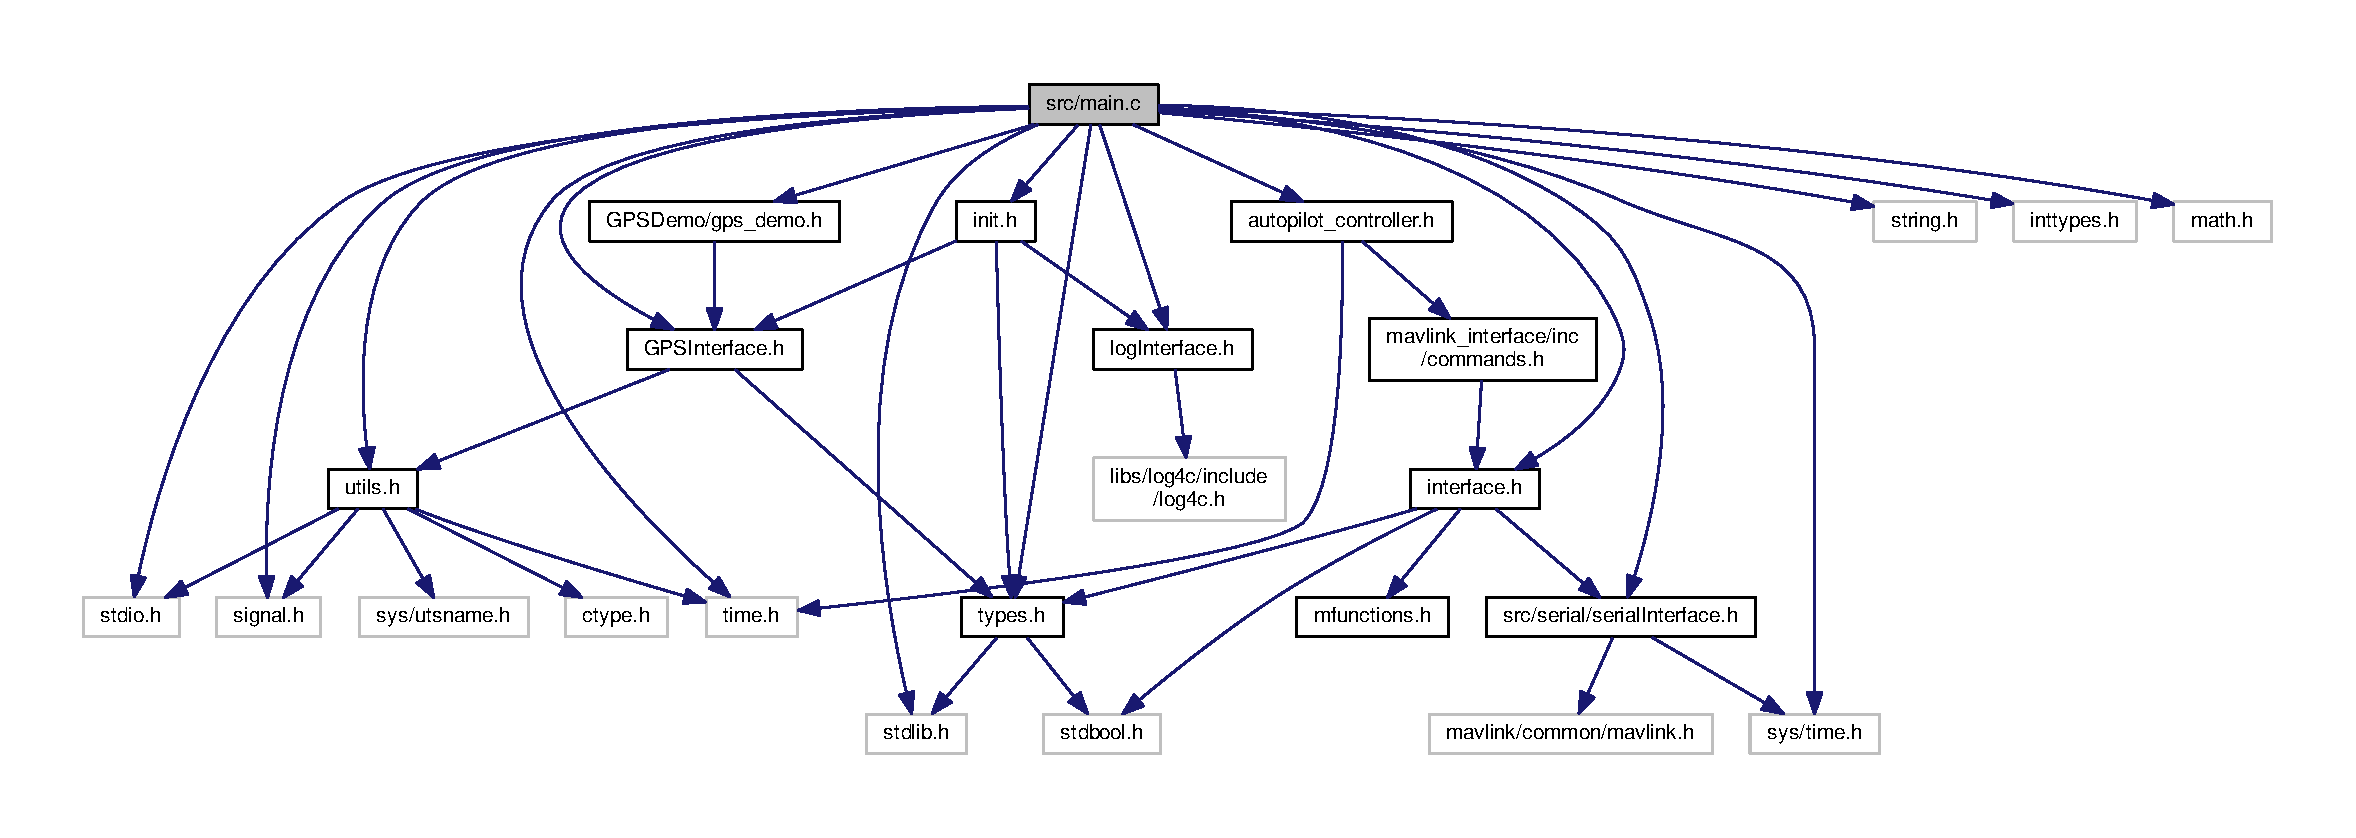
\includegraphics[width=350pt]{main_8c__incl}
\end{center}
\end{figure}
\subsection*{Functions}
\begin{DoxyCompactItemize}
\item 
int \hyperlink{main_8c_a3c04138a5bfe5d72780bb7e82a18e627}{main} (int argc, char $\ast$$\ast$argv)
\end{DoxyCompactItemize}


\subsection{Function Documentation}
\index{main.\+c@{main.\+c}!main@{main}}
\index{main@{main}!main.\+c@{main.\+c}}
\subsubsection[{\texorpdfstring{main(int argc, char $\ast$$\ast$argv)}{main(int argc, char **argv)}}]{\setlength{\rightskip}{0pt plus 5cm}int main (
\begin{DoxyParamCaption}
\item[{int}]{argc, }
\item[{char $\ast$$\ast$}]{argv}
\end{DoxyParamCaption}
)}\hypertarget{main_8c_a3c04138a5bfe5d72780bb7e82a18e627}{}\label{main_8c_a3c04138a5bfe5d72780bb7e82a18e627}

\hypertarget{main_8d}{}\section{src/main.d File Reference}
\label{main_8d}\index{src/main.\+d@{src/main.\+d}}

\hypertarget{commands_8h}{}\section{src/mavlink\+\_\+interface/inc/commands.h File Reference}
\label{commands_8h}\index{src/mavlink\+\_\+interface/inc/commands.\+h@{src/mavlink\+\_\+interface/inc/commands.\+h}}
{\ttfamily \#include \char`\"{}interface.\+h\char`\"{}}\\*
Include dependency graph for commands.\+h\+:
\nopagebreak
\begin{figure}[H]
\begin{center}
\leavevmode
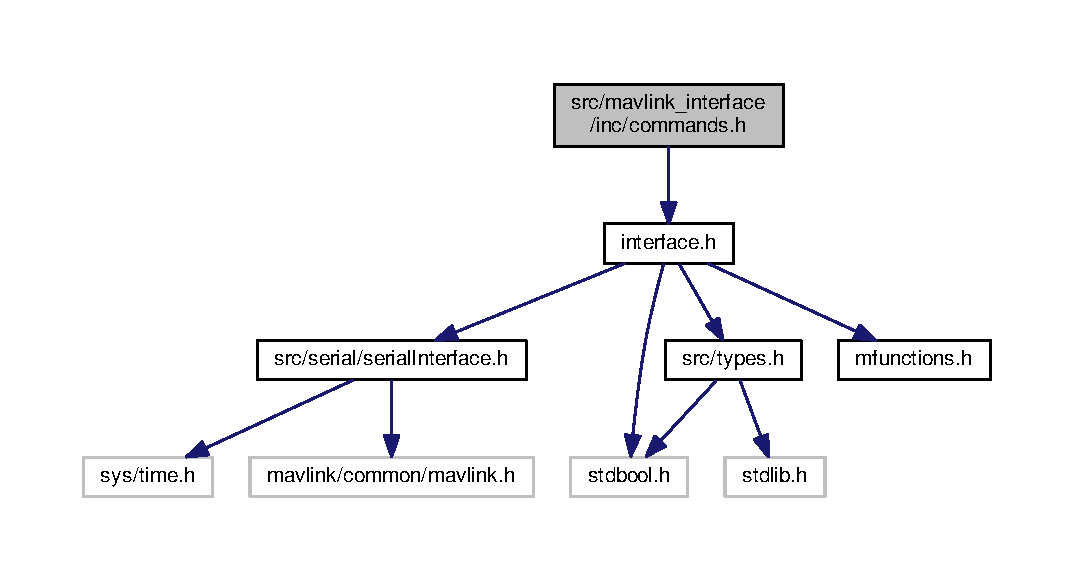
\includegraphics[width=350pt]{commands_8h__incl}
\end{center}
\end{figure}
This graph shows which files directly or indirectly include this file\+:\nopagebreak
\begin{figure}[H]
\begin{center}
\leavevmode
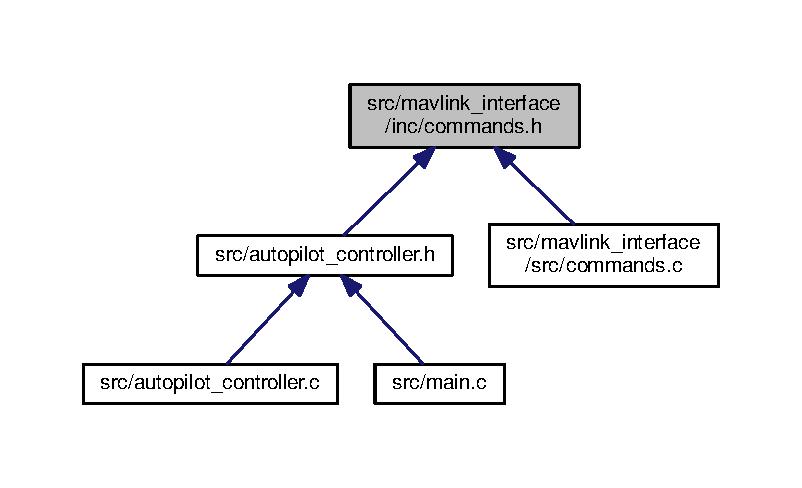
\includegraphics[width=350pt]{commands_8h__dep__incl}
\end{center}
\end{figure}
\subsection*{Macros}
\begin{DoxyCompactItemize}
\item 
\#define \hyperlink{commands_8h_abc5b6d7a209ee2018d74eb60e74d433f}{O\+F\+F\+B\+O\+A\+R\+D\+\_\+\+C\+O\+N\+T\+R\+O\+L\+\_\+\+B\+A\+S\+E\+\_\+\+M\+O\+DE}~157
\item 
\#define \hyperlink{commands_8h_a5bbd01dd6cc01d8072b4366c3bf17780}{A\+R\+M\+E\+D\+\_\+\+B\+A\+S\+E\+\_\+\+M\+O\+DE}~209
\end{DoxyCompactItemize}
\subsection*{Functions}
\begin{DoxyCompactItemize}
\item 
void \hyperlink{commands_8h_a03e9e7b262dbeae4cb8c4ae4a066531b}{operation} (float timer)
\item 
void \hyperlink{commands_8h_af36e37cab2a81a6258fcbcc6b8e28b29}{operation\+\_\+extended} (float timer)
\item 
void \hyperlink{commands_8h_a796cc160e31f24ab58c9826d316e5425}{square\+\_\+operation} (float timer)
\item 
void \hyperlink{commands_8h_a09b6928e3b393074a4435948174ae52b}{circle\+\_\+operation} (float timer)
\item 
void \hyperlink{commands_8h_aec823f3adf68cbb7a6fc0e022b85bf94}{automatic\+\_\+takeoff} (float timer, time\+\_\+t $\ast$begin)
\item 
void \hyperlink{commands_8h_a115b4a018fb4355a7f9c606b91faf9a4}{flight\+\_\+control\+\_\+sequence} (float timer)
\item 
void \hyperlink{commands_8h_a6abd769c5cbb26f123079227b2835497}{arm\+\_\+sequence} (void)
\item 
void \hyperlink{commands_8h_aa8ffb9b069939c32f2d4ae711bdca18f}{offboard\+\_\+control\+\_\+sequence} (void)
\item 
void \hyperlink{commands_8h_a0736eeabfa1f5ef6d6d5044e4e78898c}{disable\+\_\+offboard\+\_\+control\+\_\+sequence} (void)
\item 
void \hyperlink{commands_8h_a68b1b2487093eb85678440ab1629eeab}{disarm\+\_\+sequence} (void)
\item 
void \hyperlink{commands_8h_ad2d673badb605bcc66622ee8c7d7874b}{program\+\_\+counter\+\_\+sequence} (float timer, time\+\_\+t $\ast$begin)
\item 
void \hyperlink{commands_8h_a3c34d60eec74a2a54aaed0ee90a2178c}{autopilot\+\_\+write\+\_\+helper} (void)
\end{DoxyCompactItemize}
\subsection*{Variables}
\begin{DoxyCompactItemize}
\item 
mavlink\+\_\+set\+\_\+position\+\_\+target\+\_\+local\+\_\+ned\+\_\+t \hyperlink{commands_8h_a72a68d2d5fb3d88b82654a2d68377bfb}{initial\+\_\+position}
\item 
mavlink\+\_\+set\+\_\+position\+\_\+target\+\_\+local\+\_\+ned\+\_\+t \hyperlink{commands_8h_af5687cd9ba18c55c0fbe8e7d346ad8be}{ip}
\item 
\hyperlink{struct_mavlink___messages}{Mavlink\+\_\+\+Messages} \hyperlink{commands_8h_ab305999d6776734f996598fc8b065d5d}{current\+\_\+messages}
\item 
char \hyperlink{commands_8h_ac3c75d0f6f80c41ac1b5453695114156}{arm\+\_\+status}
\item 
char \hyperlink{commands_8h_a81859badc92ff83adb55fa6730145cf3}{control\+\_\+status}
\end{DoxyCompactItemize}


\subsection{Macro Definition Documentation}
\index{commands.\+h@{commands.\+h}!A\+R\+M\+E\+D\+\_\+\+B\+A\+S\+E\+\_\+\+M\+O\+DE@{A\+R\+M\+E\+D\+\_\+\+B\+A\+S\+E\+\_\+\+M\+O\+DE}}
\index{A\+R\+M\+E\+D\+\_\+\+B\+A\+S\+E\+\_\+\+M\+O\+DE@{A\+R\+M\+E\+D\+\_\+\+B\+A\+S\+E\+\_\+\+M\+O\+DE}!commands.\+h@{commands.\+h}}
\subsubsection[{\texorpdfstring{A\+R\+M\+E\+D\+\_\+\+B\+A\+S\+E\+\_\+\+M\+O\+DE}{ARMED_BASE_MODE}}]{\setlength{\rightskip}{0pt plus 5cm}\#define A\+R\+M\+E\+D\+\_\+\+B\+A\+S\+E\+\_\+\+M\+O\+DE~209}\hypertarget{commands_8h_a5bbd01dd6cc01d8072b4366c3bf17780}{}\label{commands_8h_a5bbd01dd6cc01d8072b4366c3bf17780}
\index{commands.\+h@{commands.\+h}!O\+F\+F\+B\+O\+A\+R\+D\+\_\+\+C\+O\+N\+T\+R\+O\+L\+\_\+\+B\+A\+S\+E\+\_\+\+M\+O\+DE@{O\+F\+F\+B\+O\+A\+R\+D\+\_\+\+C\+O\+N\+T\+R\+O\+L\+\_\+\+B\+A\+S\+E\+\_\+\+M\+O\+DE}}
\index{O\+F\+F\+B\+O\+A\+R\+D\+\_\+\+C\+O\+N\+T\+R\+O\+L\+\_\+\+B\+A\+S\+E\+\_\+\+M\+O\+DE@{O\+F\+F\+B\+O\+A\+R\+D\+\_\+\+C\+O\+N\+T\+R\+O\+L\+\_\+\+B\+A\+S\+E\+\_\+\+M\+O\+DE}!commands.\+h@{commands.\+h}}
\subsubsection[{\texorpdfstring{O\+F\+F\+B\+O\+A\+R\+D\+\_\+\+C\+O\+N\+T\+R\+O\+L\+\_\+\+B\+A\+S\+E\+\_\+\+M\+O\+DE}{OFFBOARD_CONTROL_BASE_MODE}}]{\setlength{\rightskip}{0pt plus 5cm}\#define O\+F\+F\+B\+O\+A\+R\+D\+\_\+\+C\+O\+N\+T\+R\+O\+L\+\_\+\+B\+A\+S\+E\+\_\+\+M\+O\+DE~157}\hypertarget{commands_8h_abc5b6d7a209ee2018d74eb60e74d433f}{}\label{commands_8h_abc5b6d7a209ee2018d74eb60e74d433f}


\subsection{Function Documentation}
\index{commands.\+h@{commands.\+h}!arm\+\_\+sequence@{arm\+\_\+sequence}}
\index{arm\+\_\+sequence@{arm\+\_\+sequence}!commands.\+h@{commands.\+h}}
\subsubsection[{\texorpdfstring{arm\+\_\+sequence(void)}{arm_sequence(void)}}]{\setlength{\rightskip}{0pt plus 5cm}void arm\+\_\+sequence (
\begin{DoxyParamCaption}
\item[{void}]{}
\end{DoxyParamCaption}
)}\hypertarget{commands_8h_a6abd769c5cbb26f123079227b2835497}{}\label{commands_8h_a6abd769c5cbb26f123079227b2835497}
\index{commands.\+h@{commands.\+h}!automatic\+\_\+takeoff@{automatic\+\_\+takeoff}}
\index{automatic\+\_\+takeoff@{automatic\+\_\+takeoff}!commands.\+h@{commands.\+h}}
\subsubsection[{\texorpdfstring{automatic\+\_\+takeoff(float timer, time\+\_\+t $\ast$begin)}{automatic_takeoff(float timer, time_t *begin)}}]{\setlength{\rightskip}{0pt plus 5cm}void automatic\+\_\+takeoff (
\begin{DoxyParamCaption}
\item[{float}]{timer, }
\item[{time\+\_\+t $\ast$}]{begin}
\end{DoxyParamCaption}
)}\hypertarget{commands_8h_aec823f3adf68cbb7a6fc0e022b85bf94}{}\label{commands_8h_aec823f3adf68cbb7a6fc0e022b85bf94}
\index{commands.\+h@{commands.\+h}!autopilot\+\_\+write\+\_\+helper@{autopilot\+\_\+write\+\_\+helper}}
\index{autopilot\+\_\+write\+\_\+helper@{autopilot\+\_\+write\+\_\+helper}!commands.\+h@{commands.\+h}}
\subsubsection[{\texorpdfstring{autopilot\+\_\+write\+\_\+helper(void)}{autopilot_write_helper(void)}}]{\setlength{\rightskip}{0pt plus 5cm}void autopilot\+\_\+write\+\_\+helper (
\begin{DoxyParamCaption}
\item[{void}]{}
\end{DoxyParamCaption}
)}\hypertarget{commands_8h_a3c34d60eec74a2a54aaed0ee90a2178c}{}\label{commands_8h_a3c34d60eec74a2a54aaed0ee90a2178c}
\index{commands.\+h@{commands.\+h}!circle\+\_\+operation@{circle\+\_\+operation}}
\index{circle\+\_\+operation@{circle\+\_\+operation}!commands.\+h@{commands.\+h}}
\subsubsection[{\texorpdfstring{circle\+\_\+operation(float timer)}{circle_operation(float timer)}}]{\setlength{\rightskip}{0pt plus 5cm}void circle\+\_\+operation (
\begin{DoxyParamCaption}
\item[{float}]{timer}
\end{DoxyParamCaption}
)}\hypertarget{commands_8h_a09b6928e3b393074a4435948174ae52b}{}\label{commands_8h_a09b6928e3b393074a4435948174ae52b}
\index{commands.\+h@{commands.\+h}!disable\+\_\+offboard\+\_\+control\+\_\+sequence@{disable\+\_\+offboard\+\_\+control\+\_\+sequence}}
\index{disable\+\_\+offboard\+\_\+control\+\_\+sequence@{disable\+\_\+offboard\+\_\+control\+\_\+sequence}!commands.\+h@{commands.\+h}}
\subsubsection[{\texorpdfstring{disable\+\_\+offboard\+\_\+control\+\_\+sequence(void)}{disable_offboard_control_sequence(void)}}]{\setlength{\rightskip}{0pt plus 5cm}void disable\+\_\+offboard\+\_\+control\+\_\+sequence (
\begin{DoxyParamCaption}
\item[{void}]{}
\end{DoxyParamCaption}
)}\hypertarget{commands_8h_a0736eeabfa1f5ef6d6d5044e4e78898c}{}\label{commands_8h_a0736eeabfa1f5ef6d6d5044e4e78898c}
\index{commands.\+h@{commands.\+h}!disarm\+\_\+sequence@{disarm\+\_\+sequence}}
\index{disarm\+\_\+sequence@{disarm\+\_\+sequence}!commands.\+h@{commands.\+h}}
\subsubsection[{\texorpdfstring{disarm\+\_\+sequence(void)}{disarm_sequence(void)}}]{\setlength{\rightskip}{0pt plus 5cm}void disarm\+\_\+sequence (
\begin{DoxyParamCaption}
\item[{void}]{}
\end{DoxyParamCaption}
)}\hypertarget{commands_8h_a68b1b2487093eb85678440ab1629eeab}{}\label{commands_8h_a68b1b2487093eb85678440ab1629eeab}
\index{commands.\+h@{commands.\+h}!flight\+\_\+control\+\_\+sequence@{flight\+\_\+control\+\_\+sequence}}
\index{flight\+\_\+control\+\_\+sequence@{flight\+\_\+control\+\_\+sequence}!commands.\+h@{commands.\+h}}
\subsubsection[{\texorpdfstring{flight\+\_\+control\+\_\+sequence(float timer)}{flight_control_sequence(float timer)}}]{\setlength{\rightskip}{0pt plus 5cm}void flight\+\_\+control\+\_\+sequence (
\begin{DoxyParamCaption}
\item[{float}]{timer}
\end{DoxyParamCaption}
)}\hypertarget{commands_8h_a115b4a018fb4355a7f9c606b91faf9a4}{}\label{commands_8h_a115b4a018fb4355a7f9c606b91faf9a4}
\index{commands.\+h@{commands.\+h}!offboard\+\_\+control\+\_\+sequence@{offboard\+\_\+control\+\_\+sequence}}
\index{offboard\+\_\+control\+\_\+sequence@{offboard\+\_\+control\+\_\+sequence}!commands.\+h@{commands.\+h}}
\subsubsection[{\texorpdfstring{offboard\+\_\+control\+\_\+sequence(void)}{offboard_control_sequence(void)}}]{\setlength{\rightskip}{0pt plus 5cm}void offboard\+\_\+control\+\_\+sequence (
\begin{DoxyParamCaption}
\item[{void}]{}
\end{DoxyParamCaption}
)}\hypertarget{commands_8h_aa8ffb9b069939c32f2d4ae711bdca18f}{}\label{commands_8h_aa8ffb9b069939c32f2d4ae711bdca18f}
\index{commands.\+h@{commands.\+h}!operation@{operation}}
\index{operation@{operation}!commands.\+h@{commands.\+h}}
\subsubsection[{\texorpdfstring{operation(float timer)}{operation(float timer)}}]{\setlength{\rightskip}{0pt plus 5cm}void operation (
\begin{DoxyParamCaption}
\item[{float}]{timer}
\end{DoxyParamCaption}
)}\hypertarget{commands_8h_a03e9e7b262dbeae4cb8c4ae4a066531b}{}\label{commands_8h_a03e9e7b262dbeae4cb8c4ae4a066531b}
\index{commands.\+h@{commands.\+h}!operation\+\_\+extended@{operation\+\_\+extended}}
\index{operation\+\_\+extended@{operation\+\_\+extended}!commands.\+h@{commands.\+h}}
\subsubsection[{\texorpdfstring{operation\+\_\+extended(float timer)}{operation_extended(float timer)}}]{\setlength{\rightskip}{0pt plus 5cm}void operation\+\_\+extended (
\begin{DoxyParamCaption}
\item[{float}]{timer}
\end{DoxyParamCaption}
)}\hypertarget{commands_8h_af36e37cab2a81a6258fcbcc6b8e28b29}{}\label{commands_8h_af36e37cab2a81a6258fcbcc6b8e28b29}
\index{commands.\+h@{commands.\+h}!program\+\_\+counter\+\_\+sequence@{program\+\_\+counter\+\_\+sequence}}
\index{program\+\_\+counter\+\_\+sequence@{program\+\_\+counter\+\_\+sequence}!commands.\+h@{commands.\+h}}
\subsubsection[{\texorpdfstring{program\+\_\+counter\+\_\+sequence(float timer, time\+\_\+t $\ast$begin)}{program_counter_sequence(float timer, time_t *begin)}}]{\setlength{\rightskip}{0pt plus 5cm}void program\+\_\+counter\+\_\+sequence (
\begin{DoxyParamCaption}
\item[{float}]{timer, }
\item[{time\+\_\+t $\ast$}]{begin}
\end{DoxyParamCaption}
)}\hypertarget{commands_8h_ad2d673badb605bcc66622ee8c7d7874b}{}\label{commands_8h_ad2d673badb605bcc66622ee8c7d7874b}
\index{commands.\+h@{commands.\+h}!square\+\_\+operation@{square\+\_\+operation}}
\index{square\+\_\+operation@{square\+\_\+operation}!commands.\+h@{commands.\+h}}
\subsubsection[{\texorpdfstring{square\+\_\+operation(float timer)}{square_operation(float timer)}}]{\setlength{\rightskip}{0pt plus 5cm}void square\+\_\+operation (
\begin{DoxyParamCaption}
\item[{float}]{timer}
\end{DoxyParamCaption}
)}\hypertarget{commands_8h_a796cc160e31f24ab58c9826d316e5425}{}\label{commands_8h_a796cc160e31f24ab58c9826d316e5425}


\subsection{Variable Documentation}
\index{commands.\+h@{commands.\+h}!arm\+\_\+status@{arm\+\_\+status}}
\index{arm\+\_\+status@{arm\+\_\+status}!commands.\+h@{commands.\+h}}
\subsubsection[{\texorpdfstring{arm\+\_\+status}{arm_status}}]{\setlength{\rightskip}{0pt plus 5cm}char arm\+\_\+status}\hypertarget{commands_8h_ac3c75d0f6f80c41ac1b5453695114156}{}\label{commands_8h_ac3c75d0f6f80c41ac1b5453695114156}
\index{commands.\+h@{commands.\+h}!control\+\_\+status@{control\+\_\+status}}
\index{control\+\_\+status@{control\+\_\+status}!commands.\+h@{commands.\+h}}
\subsubsection[{\texorpdfstring{control\+\_\+status}{control_status}}]{\setlength{\rightskip}{0pt plus 5cm}char control\+\_\+status}\hypertarget{commands_8h_a81859badc92ff83adb55fa6730145cf3}{}\label{commands_8h_a81859badc92ff83adb55fa6730145cf3}
\index{commands.\+h@{commands.\+h}!current\+\_\+messages@{current\+\_\+messages}}
\index{current\+\_\+messages@{current\+\_\+messages}!commands.\+h@{commands.\+h}}
\subsubsection[{\texorpdfstring{current\+\_\+messages}{current_messages}}]{\setlength{\rightskip}{0pt plus 5cm}{\bf Mavlink\+\_\+\+Messages} current\+\_\+messages}\hypertarget{commands_8h_ab305999d6776734f996598fc8b065d5d}{}\label{commands_8h_ab305999d6776734f996598fc8b065d5d}
\index{commands.\+h@{commands.\+h}!initial\+\_\+position@{initial\+\_\+position}}
\index{initial\+\_\+position@{initial\+\_\+position}!commands.\+h@{commands.\+h}}
\subsubsection[{\texorpdfstring{initial\+\_\+position}{initial_position}}]{\setlength{\rightskip}{0pt plus 5cm}mavlink\+\_\+set\+\_\+position\+\_\+target\+\_\+local\+\_\+ned\+\_\+t initial\+\_\+position}\hypertarget{commands_8h_a72a68d2d5fb3d88b82654a2d68377bfb}{}\label{commands_8h_a72a68d2d5fb3d88b82654a2d68377bfb}
\index{commands.\+h@{commands.\+h}!ip@{ip}}
\index{ip@{ip}!commands.\+h@{commands.\+h}}
\subsubsection[{\texorpdfstring{ip}{ip}}]{\setlength{\rightskip}{0pt plus 5cm}mavlink\+\_\+set\+\_\+position\+\_\+target\+\_\+local\+\_\+ned\+\_\+t ip}\hypertarget{commands_8h_af5687cd9ba18c55c0fbe8e7d346ad8be}{}\label{commands_8h_af5687cd9ba18c55c0fbe8e7d346ad8be}

\hypertarget{interface_8h}{}\section{src/mavlink\+\_\+interface/inc/interface.h File Reference}
\label{interface_8h}\index{src/mavlink\+\_\+interface/inc/interface.\+h@{src/mavlink\+\_\+interface/inc/interface.\+h}}
{\ttfamily \#include $<$stdbool.\+h$>$}\\*
{\ttfamily \#include $<$src/serial/serial\+Interface.\+h$>$}\\*
{\ttfamily \#include $<$src/types.\+h$>$}\\*
{\ttfamily \#include $<$mfunctions.\+h$>$}\\*
Include dependency graph for interface.\+h\+:
\nopagebreak
\begin{figure}[H]
\begin{center}
\leavevmode
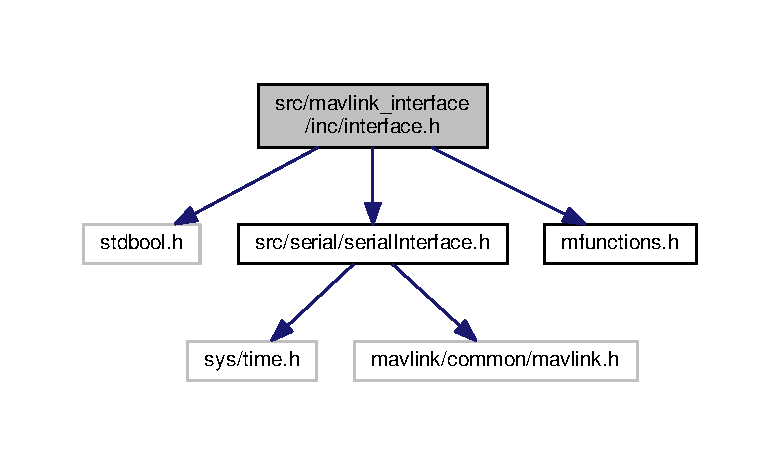
\includegraphics[width=350pt]{interface_8h__incl}
\end{center}
\end{figure}
This graph shows which files directly or indirectly include this file\+:
\nopagebreak
\begin{figure}[H]
\begin{center}
\leavevmode
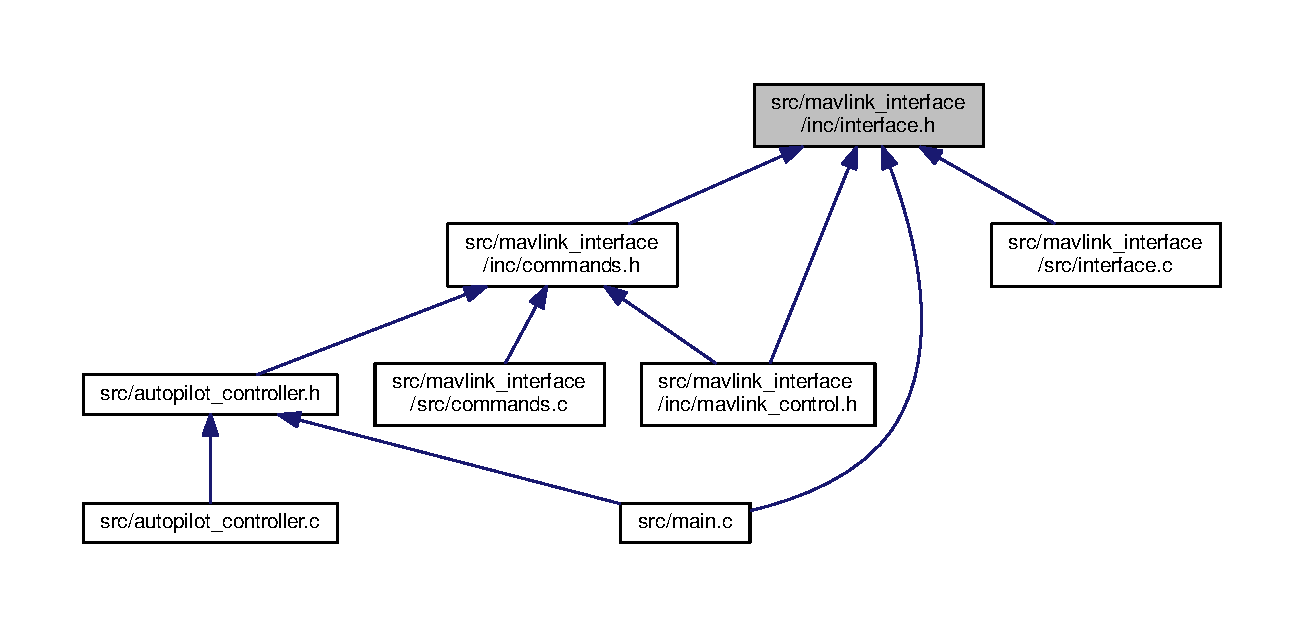
\includegraphics[width=350pt]{interface_8h__dep__incl}
\end{center}
\end{figure}
\subsection*{Data Structures}
\begin{DoxyCompactItemize}
\item 
struct \hyperlink{struct_time___stamps}{Time\+\_\+\+Stamps}
\item 
struct \hyperlink{struct_mavlink___messages}{Mavlink\+\_\+\+Messages}
\end{DoxyCompactItemize}
\subsection*{Macros}
\begin{DoxyCompactItemize}
\item 
\#define \hyperlink{interface_8h_a53c7e2d18127f70ec37b65e394185f2d}{M\+A\+V\+L\+I\+N\+K\+\_\+\+M\+S\+G\+\_\+\+S\+E\+T\+\_\+\+P\+O\+S\+I\+T\+I\+O\+N\+\_\+\+T\+A\+R\+G\+E\+T\+\_\+\+L\+O\+C\+A\+L\+\_\+\+N\+E\+D\+\_\+\+P\+O\+S\+I\+T\+I\+ON}~0b0000110111111000
\item 
\#define \hyperlink{interface_8h_acfdfbccf6175354e5129e47ed1f133a6}{M\+A\+V\+L\+I\+N\+K\+\_\+\+M\+S\+G\+\_\+\+S\+E\+T\+\_\+\+P\+O\+S\+I\+T\+I\+O\+N\+\_\+\+T\+A\+R\+G\+E\+T\+\_\+\+L\+O\+C\+A\+L\+\_\+\+N\+E\+D\+\_\+\+V\+E\+L\+O\+C\+I\+TY}~0b0000110111000111
\item 
\#define \hyperlink{interface_8h_abd9afd8b88259d73e5ef2058366ddbc4}{M\+A\+V\+L\+I\+N\+K\+\_\+\+M\+S\+G\+\_\+\+S\+E\+T\+\_\+\+P\+O\+S\+I\+T\+I\+O\+N\+\_\+\+T\+A\+R\+G\+E\+T\+\_\+\+L\+O\+C\+A\+L\+\_\+\+N\+E\+D\+\_\+\+A\+C\+C\+E\+L\+E\+R\+A\+T\+I\+ON}~0b0000110000111111
\item 
\#define \hyperlink{interface_8h_abad42a51b8b2462c753b25d53fcec7fb}{M\+A\+V\+L\+I\+N\+K\+\_\+\+M\+S\+G\+\_\+\+S\+E\+T\+\_\+\+P\+O\+S\+I\+T\+I\+O\+N\+\_\+\+T\+A\+R\+G\+E\+T\+\_\+\+L\+O\+C\+A\+L\+\_\+\+N\+E\+D\+\_\+\+F\+O\+R\+CE}~0b0000111000111111
\item 
\#define \hyperlink{interface_8h_aa53ad3b098f8407d8a2c9672a44dac7d}{M\+A\+V\+L\+I\+N\+K\+\_\+\+M\+S\+G\+\_\+\+S\+E\+T\+\_\+\+P\+O\+S\+I\+T\+I\+O\+N\+\_\+\+T\+A\+R\+G\+E\+T\+\_\+\+L\+O\+C\+A\+L\+\_\+\+N\+E\+D\+\_\+\+Y\+A\+W\+\_\+\+A\+N\+G\+LE}~0b0000100111111111
\item 
\#define \hyperlink{interface_8h_a5bd29412a96cb9ac218625952a5608c4}{M\+A\+V\+L\+I\+N\+K\+\_\+\+M\+S\+G\+\_\+\+S\+E\+T\+\_\+\+P\+O\+S\+I\+T\+I\+O\+N\+\_\+\+T\+A\+R\+G\+E\+T\+\_\+\+L\+O\+C\+A\+L\+\_\+\+N\+E\+D\+\_\+\+Y\+A\+W\+\_\+\+R\+A\+TE}~0b0000010111111111
\end{DoxyCompactItemize}
\subsection*{Typedefs}
\begin{DoxyCompactItemize}
\item 
typedef struct \hyperlink{struct_time___stamps}{Time\+\_\+\+Stamps} \hyperlink{interface_8h_a3eab1bf5782c05897f4da1f44b727016}{Time\+\_\+\+Stamps}
\item 
typedef struct \hyperlink{struct_mavlink___messages}{Mavlink\+\_\+\+Messages} \hyperlink{interface_8h_a5a6ca3ba0abb750a1c3ece47c50718ad}{Mavlink\+\_\+\+Messages}
\end{DoxyCompactItemize}
\subsection*{Functions}
\begin{DoxyCompactItemize}
\item 
void \hyperlink{interface_8h_aa0bcb2f31d5df71593891fbacb8ff20a}{reset\+\_\+timestamps} (\hyperlink{struct_time___stamps}{Time\+\_\+\+Stamps} $\ast$ts)
\begin{DoxyCompactList}\small\item\em Zeros out all the timestamps. \end{DoxyCompactList}\item 
void \hyperlink{interface_8h_aa4bd4ad9917c2577168def15cf9aefb7}{autopilot\+\_\+initialize} (void)
\begin{DoxyCompactList}\small\item\em Initialize system-\/wide important parameters and flags. \end{DoxyCompactList}\item 
void \hyperlink{interface_8h_aeeb66c18def4c2bb8c404a75ccf4ff07}{autopilot\+\_\+start} (void)
\begin{DoxyCompactList}\small\item\em Used to define the initial position. This method is supposed to be called once on startup after the first call to read\+\_\+message() (which listens for a position message from the autopilot). \end{DoxyCompactList}\item 
void \hyperlink{interface_8h_a761018fc7556aac6d6f302b7406f791d}{read\+\_\+messages} (void)
\begin{DoxyCompactList}\small\item\em Reads M\+A\+V\+Link messages from the autopilot until all requested messages are received (this is controlled by the received\+\_\+all flag inside the function). The received messages are set in the \hyperlink{struct_mavlink___messages}{Mavlink\+\_\+\+Messages}. This method is blocking and will not exit until all requested messages are obtained (may become an infinite loop). \end{DoxyCompactList}\item 
void \hyperlink{interface_8h_aa400b6caf4a262ea4446854e90ab005d}{autopilot\+\_\+write} (void)
\begin{DoxyCompactList}\small\item\em A \char`\"{}dummy\char`\"{} method that writes a void (all zeros) setpoint to the autopilot. Used to signal startup. \end{DoxyCompactList}\item 
void \hyperlink{interface_8h_ac8fa807910345b796fe4fd9f61101ba2}{autopilot\+\_\+write\+\_\+message} (mavlink\+\_\+message\+\_\+t message)
\begin{DoxyCompactList}\small\item\em Write a M\+A\+V\+Link message to the autopilot. \end{DoxyCompactList}\item 
void \hyperlink{interface_8h_ab2559012cba7e4c72ec10a59c87f84cb}{autopilot\+\_\+write\+\_\+setpoint} (void)
\begin{DoxyCompactList}\small\item\em Write the current setpoint to the autopilot after it\textquotesingle{}s been updated (needs to be called explicitly) \end{DoxyCompactList}\item 
void \hyperlink{interface_8h_a7a3598bf63d9844fcd22328fc63842a4}{autopilot\+\_\+update\+\_\+setpoint} (mavlink\+\_\+set\+\_\+position\+\_\+target\+\_\+local\+\_\+ned\+\_\+t setpoint)
\begin{DoxyCompactList}\small\item\em Update the current setpoint with the given setpoint. \end{DoxyCompactList}\item 
bool \hyperlink{interface_8h_a4b3151ecef548d647281eba568170280}{disable\+\_\+offboard\+\_\+control} (void)
\begin{DoxyCompactList}\small\item\em Disabled the offboard control of the autopilot. \end{DoxyCompactList}\item 
bool \hyperlink{interface_8h_a6f0b501cf0b9b1e74c0053df49b3bdc6}{enable\+\_\+offboard\+\_\+control} (void)
\begin{DoxyCompactList}\small\item\em Enables the offboard control of the autopilot, setting the appropriate flag. \end{DoxyCompactList}\item 
int \hyperlink{interface_8h_a22fb091245542a81979c3d517c048d9c}{toggle\+\_\+offboard\+\_\+control} (bool flag)
\begin{DoxyCompactList}\small\item\em The function that\textquotesingle{}s used by enable/disable\+\_\+offbard\+\_\+control() to actually write the appropriate command to the autopilot. \end{DoxyCompactList}\item 
void \hyperlink{interface_8h_ae4ffa041a7021553ce57bcc004721afe}{autopilot\+\_\+arm} (void)
\begin{DoxyCompactList}\small\item\em Arm the autopilot. \end{DoxyCompactList}\item 
void \hyperlink{interface_8h_ab784fd6af4d00965889893c0cf462f26}{autopilot\+\_\+disarm} (void)
\begin{DoxyCompactList}\small\item\em Disarm the autopilot. \end{DoxyCompactList}\item 
int \hyperlink{interface_8h_ae2645ae25eb4ac098eb579dd9a49c1b9}{toggle\+\_\+arm\+\_\+disarm} (bool flag)
\begin{DoxyCompactList}\small\item\em Used by autopilot\+\_\+arm/disarm() in a similar manner to toogle\+\_\+offboard\+\_\+control(). \end{DoxyCompactList}\item 
int \hyperlink{interface_8h_a56a6826eb5bf8127144d09ecfa6bee9a}{check\+\_\+offboard\+\_\+control} (void)
\begin{DoxyCompactList}\small\item\em A convenience function to check if the autopilot is in offboard control or not. \end{DoxyCompactList}\item 
int \hyperlink{interface_8h_a8140deb719d9d4350a97d225d1d2cd04}{check\+\_\+arm\+\_\+disarm} (void)
\begin{DoxyCompactList}\small\item\em Similar to \hyperlink{interface_8h_a56a6826eb5bf8127144d09ecfa6bee9a}{check\+\_\+offboard\+\_\+control()}. \end{DoxyCompactList}\item 
int \hyperlink{interface_8h_a778200ebd979982133bd3965e49976a5}{check\+\_\+message} (uint16\+\_\+t C\+O\+M\+M\+A\+N\+D\+\_\+\+ID)
\begin{DoxyCompactList}\small\item\em The function that\textquotesingle{}s used by \hyperlink{interface_8h_a56a6826eb5bf8127144d09ecfa6bee9a}{check\+\_\+offboard\+\_\+control()} and \hyperlink{interface_8h_a8140deb719d9d4350a97d225d1d2cd04}{check\+\_\+arm\+\_\+disarm()} to determine the status. \end{DoxyCompactList}\item 
int \hyperlink{interface_8h_a2c968172095b29933cf3b8997e2cb140}{get\+\_\+gps\+\_\+from\+\_\+autopilot} (\hyperlink{struct_full_g_p_s_data}{Full\+G\+P\+S\+Data} $\ast$gps\+Data)
\begin{DoxyCompactList}\small\item\em Update the \hyperlink{struct_full_g_p_s_data}{Full\+G\+P\+S\+Data} based on information from the G\+L\+O\+B\+A\+L\+\_\+\+P\+O\+S\+I\+T\+I\+O\+N\+\_\+\+I\+N\+T\+\_\+\+C\+OV message. \end{DoxyCompactList}\item 
int \hyperlink{interface_8h_a8f2570bef0f8d567d0eee6648951a9bb}{pre\+\_\+arm\+\_\+void\+\_\+commands} ()
\begin{DoxyCompactList}\small\item\em Used to send \char`\"{}dummy\char`\"{} setpoints to the autopilot. This method is meant to be used before switching to offboard mode. It\textquotesingle{}s required that the setpoint streaming will already begin before switching to offboard, otherwise the autopilot will reject the mode switch. \end{DoxyCompactList}\item 
int \hyperlink{interface_8h_a6ea50ba9fe9c2ae23ab9cbc9a1a6adda}{autopilot\+\_\+ok} ()
\begin{DoxyCompactList}\small\item\em Receive a H\+E\+A\+R\+T\+B\+E\+AT message from the autopilot. Used to verify that the autopilot is up and running and is connected. \end{DoxyCompactList}\item 
void \hyperlink{interface_8h_a93e3fdd06c6bbc40c6fb045ba1a29bb6}{set\+\_\+position} (float x, float y, float z, mavlink\+\_\+set\+\_\+position\+\_\+target\+\_\+local\+\_\+ned\+\_\+t $\ast$sp)
\item 
void \hyperlink{interface_8h_a992ee3c0025abb2bba96ed4bb7277484}{set\+\_\+\+\_\+} (float x, float y, float z, mavlink\+\_\+set\+\_\+position\+\_\+target\+\_\+local\+\_\+ned\+\_\+t $\ast$set\+\_\+point)
\item 
void \hyperlink{interface_8h_a7e5983c2d9a0bd9837d1809bcb7481db}{set\+\_\+velocity} (float vx, float vy, float va, mavlink\+\_\+set\+\_\+position\+\_\+target\+\_\+local\+\_\+ned\+\_\+t $\ast$set\+\_\+point)
\item 
void \hyperlink{interface_8h_ad089b2003c05af61daf45a455dba3c65}{set\+\_\+yaw} (float yaw, mavlink\+\_\+set\+\_\+position\+\_\+target\+\_\+local\+\_\+ned\+\_\+t $\ast$sp)
\item 
void \hyperlink{interface_8h_aaf2bde2dc6e6e3ea59ddd5e36549f3ab}{position\+\_\+and\+\_\+speed\+\_\+set} (float x, float y, float z, float vx, float vy, float vz, mavlink\+\_\+set\+\_\+position\+\_\+target\+\_\+local\+\_\+ned\+\_\+t $\ast$final\+\_\+set\+\_\+point)
\item 
void \hyperlink{interface_8h_a66e1f11d723feacc42bbca4020f3a858}{set\+\_\+circle} (float R, float theta, float z, mavlink\+\_\+set\+\_\+position\+\_\+target\+\_\+local\+\_\+ned\+\_\+t $\ast$set\+\_\+point)
\item 
uint64\+\_\+t \hyperlink{interface_8h_a2ac9437af95602ce4e5ba39be2d2429b}{get\+\_\+time\+\_\+usec} (void)
\end{DoxyCompactItemize}


\subsection{Detailed Description}
\begin{DoxyAuthor}{Author}
Trent Lukaczyk, \href{mailto:aerialhedgehog@gmail.com}{\tt aerialhedgehog@gmail.\+com} 

Jaycee Lock, \href{mailto:jaycee.lock@gmail.com}{\tt jaycee.\+lock@gmail.\+com} 

Lorenz Meier, \href{mailto:lm@inf.ethz.ch}{\tt lm@inf.\+ethz.\+ch}
\end{DoxyAuthor}
Modifications made by \+: Mohamed Hage Hassan, \href{mailto:mohamed.hagehassan@yahoo.com}{\tt mohamed.\+hagehassan@yahoo.\+com} 

\subsection{Macro Definition Documentation}
\index{interface.\+h@{interface.\+h}!M\+A\+V\+L\+I\+N\+K\+\_\+\+M\+S\+G\+\_\+\+S\+E\+T\+\_\+\+P\+O\+S\+I\+T\+I\+O\+N\+\_\+\+T\+A\+R\+G\+E\+T\+\_\+\+L\+O\+C\+A\+L\+\_\+\+N\+E\+D\+\_\+\+A\+C\+C\+E\+L\+E\+R\+A\+T\+I\+ON@{M\+A\+V\+L\+I\+N\+K\+\_\+\+M\+S\+G\+\_\+\+S\+E\+T\+\_\+\+P\+O\+S\+I\+T\+I\+O\+N\+\_\+\+T\+A\+R\+G\+E\+T\+\_\+\+L\+O\+C\+A\+L\+\_\+\+N\+E\+D\+\_\+\+A\+C\+C\+E\+L\+E\+R\+A\+T\+I\+ON}}
\index{M\+A\+V\+L\+I\+N\+K\+\_\+\+M\+S\+G\+\_\+\+S\+E\+T\+\_\+\+P\+O\+S\+I\+T\+I\+O\+N\+\_\+\+T\+A\+R\+G\+E\+T\+\_\+\+L\+O\+C\+A\+L\+\_\+\+N\+E\+D\+\_\+\+A\+C\+C\+E\+L\+E\+R\+A\+T\+I\+ON@{M\+A\+V\+L\+I\+N\+K\+\_\+\+M\+S\+G\+\_\+\+S\+E\+T\+\_\+\+P\+O\+S\+I\+T\+I\+O\+N\+\_\+\+T\+A\+R\+G\+E\+T\+\_\+\+L\+O\+C\+A\+L\+\_\+\+N\+E\+D\+\_\+\+A\+C\+C\+E\+L\+E\+R\+A\+T\+I\+ON}!interface.\+h@{interface.\+h}}
\subsubsection[{\texorpdfstring{M\+A\+V\+L\+I\+N\+K\+\_\+\+M\+S\+G\+\_\+\+S\+E\+T\+\_\+\+P\+O\+S\+I\+T\+I\+O\+N\+\_\+\+T\+A\+R\+G\+E\+T\+\_\+\+L\+O\+C\+A\+L\+\_\+\+N\+E\+D\+\_\+\+A\+C\+C\+E\+L\+E\+R\+A\+T\+I\+ON}{MAVLINK_MSG_SET_POSITION_TARGET_LOCAL_NED_ACCELERATION}}]{\setlength{\rightskip}{0pt plus 5cm}\#define M\+A\+V\+L\+I\+N\+K\+\_\+\+M\+S\+G\+\_\+\+S\+E\+T\+\_\+\+P\+O\+S\+I\+T\+I\+O\+N\+\_\+\+T\+A\+R\+G\+E\+T\+\_\+\+L\+O\+C\+A\+L\+\_\+\+N\+E\+D\+\_\+\+A\+C\+C\+E\+L\+E\+R\+A\+T\+I\+ON~0b0000110000111111}\hypertarget{interface_8h_abd9afd8b88259d73e5ef2058366ddbc4}{}\label{interface_8h_abd9afd8b88259d73e5ef2058366ddbc4}
\index{interface.\+h@{interface.\+h}!M\+A\+V\+L\+I\+N\+K\+\_\+\+M\+S\+G\+\_\+\+S\+E\+T\+\_\+\+P\+O\+S\+I\+T\+I\+O\+N\+\_\+\+T\+A\+R\+G\+E\+T\+\_\+\+L\+O\+C\+A\+L\+\_\+\+N\+E\+D\+\_\+\+F\+O\+R\+CE@{M\+A\+V\+L\+I\+N\+K\+\_\+\+M\+S\+G\+\_\+\+S\+E\+T\+\_\+\+P\+O\+S\+I\+T\+I\+O\+N\+\_\+\+T\+A\+R\+G\+E\+T\+\_\+\+L\+O\+C\+A\+L\+\_\+\+N\+E\+D\+\_\+\+F\+O\+R\+CE}}
\index{M\+A\+V\+L\+I\+N\+K\+\_\+\+M\+S\+G\+\_\+\+S\+E\+T\+\_\+\+P\+O\+S\+I\+T\+I\+O\+N\+\_\+\+T\+A\+R\+G\+E\+T\+\_\+\+L\+O\+C\+A\+L\+\_\+\+N\+E\+D\+\_\+\+F\+O\+R\+CE@{M\+A\+V\+L\+I\+N\+K\+\_\+\+M\+S\+G\+\_\+\+S\+E\+T\+\_\+\+P\+O\+S\+I\+T\+I\+O\+N\+\_\+\+T\+A\+R\+G\+E\+T\+\_\+\+L\+O\+C\+A\+L\+\_\+\+N\+E\+D\+\_\+\+F\+O\+R\+CE}!interface.\+h@{interface.\+h}}
\subsubsection[{\texorpdfstring{M\+A\+V\+L\+I\+N\+K\+\_\+\+M\+S\+G\+\_\+\+S\+E\+T\+\_\+\+P\+O\+S\+I\+T\+I\+O\+N\+\_\+\+T\+A\+R\+G\+E\+T\+\_\+\+L\+O\+C\+A\+L\+\_\+\+N\+E\+D\+\_\+\+F\+O\+R\+CE}{MAVLINK_MSG_SET_POSITION_TARGET_LOCAL_NED_FORCE}}]{\setlength{\rightskip}{0pt plus 5cm}\#define M\+A\+V\+L\+I\+N\+K\+\_\+\+M\+S\+G\+\_\+\+S\+E\+T\+\_\+\+P\+O\+S\+I\+T\+I\+O\+N\+\_\+\+T\+A\+R\+G\+E\+T\+\_\+\+L\+O\+C\+A\+L\+\_\+\+N\+E\+D\+\_\+\+F\+O\+R\+CE~0b0000111000111111}\hypertarget{interface_8h_abad42a51b8b2462c753b25d53fcec7fb}{}\label{interface_8h_abad42a51b8b2462c753b25d53fcec7fb}
\index{interface.\+h@{interface.\+h}!M\+A\+V\+L\+I\+N\+K\+\_\+\+M\+S\+G\+\_\+\+S\+E\+T\+\_\+\+P\+O\+S\+I\+T\+I\+O\+N\+\_\+\+T\+A\+R\+G\+E\+T\+\_\+\+L\+O\+C\+A\+L\+\_\+\+N\+E\+D\+\_\+\+P\+O\+S\+I\+T\+I\+ON@{M\+A\+V\+L\+I\+N\+K\+\_\+\+M\+S\+G\+\_\+\+S\+E\+T\+\_\+\+P\+O\+S\+I\+T\+I\+O\+N\+\_\+\+T\+A\+R\+G\+E\+T\+\_\+\+L\+O\+C\+A\+L\+\_\+\+N\+E\+D\+\_\+\+P\+O\+S\+I\+T\+I\+ON}}
\index{M\+A\+V\+L\+I\+N\+K\+\_\+\+M\+S\+G\+\_\+\+S\+E\+T\+\_\+\+P\+O\+S\+I\+T\+I\+O\+N\+\_\+\+T\+A\+R\+G\+E\+T\+\_\+\+L\+O\+C\+A\+L\+\_\+\+N\+E\+D\+\_\+\+P\+O\+S\+I\+T\+I\+ON@{M\+A\+V\+L\+I\+N\+K\+\_\+\+M\+S\+G\+\_\+\+S\+E\+T\+\_\+\+P\+O\+S\+I\+T\+I\+O\+N\+\_\+\+T\+A\+R\+G\+E\+T\+\_\+\+L\+O\+C\+A\+L\+\_\+\+N\+E\+D\+\_\+\+P\+O\+S\+I\+T\+I\+ON}!interface.\+h@{interface.\+h}}
\subsubsection[{\texorpdfstring{M\+A\+V\+L\+I\+N\+K\+\_\+\+M\+S\+G\+\_\+\+S\+E\+T\+\_\+\+P\+O\+S\+I\+T\+I\+O\+N\+\_\+\+T\+A\+R\+G\+E\+T\+\_\+\+L\+O\+C\+A\+L\+\_\+\+N\+E\+D\+\_\+\+P\+O\+S\+I\+T\+I\+ON}{MAVLINK_MSG_SET_POSITION_TARGET_LOCAL_NED_POSITION}}]{\setlength{\rightskip}{0pt plus 5cm}\#define M\+A\+V\+L\+I\+N\+K\+\_\+\+M\+S\+G\+\_\+\+S\+E\+T\+\_\+\+P\+O\+S\+I\+T\+I\+O\+N\+\_\+\+T\+A\+R\+G\+E\+T\+\_\+\+L\+O\+C\+A\+L\+\_\+\+N\+E\+D\+\_\+\+P\+O\+S\+I\+T\+I\+ON~0b0000110111111000}\hypertarget{interface_8h_a53c7e2d18127f70ec37b65e394185f2d}{}\label{interface_8h_a53c7e2d18127f70ec37b65e394185f2d}
\index{interface.\+h@{interface.\+h}!M\+A\+V\+L\+I\+N\+K\+\_\+\+M\+S\+G\+\_\+\+S\+E\+T\+\_\+\+P\+O\+S\+I\+T\+I\+O\+N\+\_\+\+T\+A\+R\+G\+E\+T\+\_\+\+L\+O\+C\+A\+L\+\_\+\+N\+E\+D\+\_\+\+V\+E\+L\+O\+C\+I\+TY@{M\+A\+V\+L\+I\+N\+K\+\_\+\+M\+S\+G\+\_\+\+S\+E\+T\+\_\+\+P\+O\+S\+I\+T\+I\+O\+N\+\_\+\+T\+A\+R\+G\+E\+T\+\_\+\+L\+O\+C\+A\+L\+\_\+\+N\+E\+D\+\_\+\+V\+E\+L\+O\+C\+I\+TY}}
\index{M\+A\+V\+L\+I\+N\+K\+\_\+\+M\+S\+G\+\_\+\+S\+E\+T\+\_\+\+P\+O\+S\+I\+T\+I\+O\+N\+\_\+\+T\+A\+R\+G\+E\+T\+\_\+\+L\+O\+C\+A\+L\+\_\+\+N\+E\+D\+\_\+\+V\+E\+L\+O\+C\+I\+TY@{M\+A\+V\+L\+I\+N\+K\+\_\+\+M\+S\+G\+\_\+\+S\+E\+T\+\_\+\+P\+O\+S\+I\+T\+I\+O\+N\+\_\+\+T\+A\+R\+G\+E\+T\+\_\+\+L\+O\+C\+A\+L\+\_\+\+N\+E\+D\+\_\+\+V\+E\+L\+O\+C\+I\+TY}!interface.\+h@{interface.\+h}}
\subsubsection[{\texorpdfstring{M\+A\+V\+L\+I\+N\+K\+\_\+\+M\+S\+G\+\_\+\+S\+E\+T\+\_\+\+P\+O\+S\+I\+T\+I\+O\+N\+\_\+\+T\+A\+R\+G\+E\+T\+\_\+\+L\+O\+C\+A\+L\+\_\+\+N\+E\+D\+\_\+\+V\+E\+L\+O\+C\+I\+TY}{MAVLINK_MSG_SET_POSITION_TARGET_LOCAL_NED_VELOCITY}}]{\setlength{\rightskip}{0pt plus 5cm}\#define M\+A\+V\+L\+I\+N\+K\+\_\+\+M\+S\+G\+\_\+\+S\+E\+T\+\_\+\+P\+O\+S\+I\+T\+I\+O\+N\+\_\+\+T\+A\+R\+G\+E\+T\+\_\+\+L\+O\+C\+A\+L\+\_\+\+N\+E\+D\+\_\+\+V\+E\+L\+O\+C\+I\+TY~0b0000110111000111}\hypertarget{interface_8h_acfdfbccf6175354e5129e47ed1f133a6}{}\label{interface_8h_acfdfbccf6175354e5129e47ed1f133a6}
\index{interface.\+h@{interface.\+h}!M\+A\+V\+L\+I\+N\+K\+\_\+\+M\+S\+G\+\_\+\+S\+E\+T\+\_\+\+P\+O\+S\+I\+T\+I\+O\+N\+\_\+\+T\+A\+R\+G\+E\+T\+\_\+\+L\+O\+C\+A\+L\+\_\+\+N\+E\+D\+\_\+\+Y\+A\+W\+\_\+\+A\+N\+G\+LE@{M\+A\+V\+L\+I\+N\+K\+\_\+\+M\+S\+G\+\_\+\+S\+E\+T\+\_\+\+P\+O\+S\+I\+T\+I\+O\+N\+\_\+\+T\+A\+R\+G\+E\+T\+\_\+\+L\+O\+C\+A\+L\+\_\+\+N\+E\+D\+\_\+\+Y\+A\+W\+\_\+\+A\+N\+G\+LE}}
\index{M\+A\+V\+L\+I\+N\+K\+\_\+\+M\+S\+G\+\_\+\+S\+E\+T\+\_\+\+P\+O\+S\+I\+T\+I\+O\+N\+\_\+\+T\+A\+R\+G\+E\+T\+\_\+\+L\+O\+C\+A\+L\+\_\+\+N\+E\+D\+\_\+\+Y\+A\+W\+\_\+\+A\+N\+G\+LE@{M\+A\+V\+L\+I\+N\+K\+\_\+\+M\+S\+G\+\_\+\+S\+E\+T\+\_\+\+P\+O\+S\+I\+T\+I\+O\+N\+\_\+\+T\+A\+R\+G\+E\+T\+\_\+\+L\+O\+C\+A\+L\+\_\+\+N\+E\+D\+\_\+\+Y\+A\+W\+\_\+\+A\+N\+G\+LE}!interface.\+h@{interface.\+h}}
\subsubsection[{\texorpdfstring{M\+A\+V\+L\+I\+N\+K\+\_\+\+M\+S\+G\+\_\+\+S\+E\+T\+\_\+\+P\+O\+S\+I\+T\+I\+O\+N\+\_\+\+T\+A\+R\+G\+E\+T\+\_\+\+L\+O\+C\+A\+L\+\_\+\+N\+E\+D\+\_\+\+Y\+A\+W\+\_\+\+A\+N\+G\+LE}{MAVLINK_MSG_SET_POSITION_TARGET_LOCAL_NED_YAW_ANGLE}}]{\setlength{\rightskip}{0pt plus 5cm}\#define M\+A\+V\+L\+I\+N\+K\+\_\+\+M\+S\+G\+\_\+\+S\+E\+T\+\_\+\+P\+O\+S\+I\+T\+I\+O\+N\+\_\+\+T\+A\+R\+G\+E\+T\+\_\+\+L\+O\+C\+A\+L\+\_\+\+N\+E\+D\+\_\+\+Y\+A\+W\+\_\+\+A\+N\+G\+LE~0b0000100111111111}\hypertarget{interface_8h_aa53ad3b098f8407d8a2c9672a44dac7d}{}\label{interface_8h_aa53ad3b098f8407d8a2c9672a44dac7d}
\index{interface.\+h@{interface.\+h}!M\+A\+V\+L\+I\+N\+K\+\_\+\+M\+S\+G\+\_\+\+S\+E\+T\+\_\+\+P\+O\+S\+I\+T\+I\+O\+N\+\_\+\+T\+A\+R\+G\+E\+T\+\_\+\+L\+O\+C\+A\+L\+\_\+\+N\+E\+D\+\_\+\+Y\+A\+W\+\_\+\+R\+A\+TE@{M\+A\+V\+L\+I\+N\+K\+\_\+\+M\+S\+G\+\_\+\+S\+E\+T\+\_\+\+P\+O\+S\+I\+T\+I\+O\+N\+\_\+\+T\+A\+R\+G\+E\+T\+\_\+\+L\+O\+C\+A\+L\+\_\+\+N\+E\+D\+\_\+\+Y\+A\+W\+\_\+\+R\+A\+TE}}
\index{M\+A\+V\+L\+I\+N\+K\+\_\+\+M\+S\+G\+\_\+\+S\+E\+T\+\_\+\+P\+O\+S\+I\+T\+I\+O\+N\+\_\+\+T\+A\+R\+G\+E\+T\+\_\+\+L\+O\+C\+A\+L\+\_\+\+N\+E\+D\+\_\+\+Y\+A\+W\+\_\+\+R\+A\+TE@{M\+A\+V\+L\+I\+N\+K\+\_\+\+M\+S\+G\+\_\+\+S\+E\+T\+\_\+\+P\+O\+S\+I\+T\+I\+O\+N\+\_\+\+T\+A\+R\+G\+E\+T\+\_\+\+L\+O\+C\+A\+L\+\_\+\+N\+E\+D\+\_\+\+Y\+A\+W\+\_\+\+R\+A\+TE}!interface.\+h@{interface.\+h}}
\subsubsection[{\texorpdfstring{M\+A\+V\+L\+I\+N\+K\+\_\+\+M\+S\+G\+\_\+\+S\+E\+T\+\_\+\+P\+O\+S\+I\+T\+I\+O\+N\+\_\+\+T\+A\+R\+G\+E\+T\+\_\+\+L\+O\+C\+A\+L\+\_\+\+N\+E\+D\+\_\+\+Y\+A\+W\+\_\+\+R\+A\+TE}{MAVLINK_MSG_SET_POSITION_TARGET_LOCAL_NED_YAW_RATE}}]{\setlength{\rightskip}{0pt plus 5cm}\#define M\+A\+V\+L\+I\+N\+K\+\_\+\+M\+S\+G\+\_\+\+S\+E\+T\+\_\+\+P\+O\+S\+I\+T\+I\+O\+N\+\_\+\+T\+A\+R\+G\+E\+T\+\_\+\+L\+O\+C\+A\+L\+\_\+\+N\+E\+D\+\_\+\+Y\+A\+W\+\_\+\+R\+A\+TE~0b0000010111111111}\hypertarget{interface_8h_a5bd29412a96cb9ac218625952a5608c4}{}\label{interface_8h_a5bd29412a96cb9ac218625952a5608c4}


\subsection{Typedef Documentation}
\index{interface.\+h@{interface.\+h}!Mavlink\+\_\+\+Messages@{Mavlink\+\_\+\+Messages}}
\index{Mavlink\+\_\+\+Messages@{Mavlink\+\_\+\+Messages}!interface.\+h@{interface.\+h}}
\subsubsection[{\texorpdfstring{Mavlink\+\_\+\+Messages}{Mavlink_Messages}}]{\setlength{\rightskip}{0pt plus 5cm}typedef struct {\bf Mavlink\+\_\+\+Messages}  {\bf Mavlink\+\_\+\+Messages}}\hypertarget{interface_8h_a5a6ca3ba0abb750a1c3ece47c50718ad}{}\label{interface_8h_a5a6ca3ba0abb750a1c3ece47c50718ad}
Holds the last messages that were received from the autopilot \index{interface.\+h@{interface.\+h}!Time\+\_\+\+Stamps@{Time\+\_\+\+Stamps}}
\index{Time\+\_\+\+Stamps@{Time\+\_\+\+Stamps}!interface.\+h@{interface.\+h}}
\subsubsection[{\texorpdfstring{Time\+\_\+\+Stamps}{Time_Stamps}}]{\setlength{\rightskip}{0pt plus 5cm}typedef struct {\bf Time\+\_\+\+Stamps}  {\bf Time\+\_\+\+Stamps}}\hypertarget{interface_8h_a3eab1bf5782c05897f4da1f44b727016}{}\label{interface_8h_a3eab1bf5782c05897f4da1f44b727016}
timestamps of every message in Mavlink\+\_\+\+Messagess 

\subsection{Function Documentation}
\index{interface.\+h@{interface.\+h}!autopilot\+\_\+arm@{autopilot\+\_\+arm}}
\index{autopilot\+\_\+arm@{autopilot\+\_\+arm}!interface.\+h@{interface.\+h}}
\subsubsection[{\texorpdfstring{autopilot\+\_\+arm(void)}{autopilot_arm(void)}}]{\setlength{\rightskip}{0pt plus 5cm}void autopilot\+\_\+arm (
\begin{DoxyParamCaption}
\item[{void}]{}
\end{DoxyParamCaption}
)}\hypertarget{interface_8h_ae4ffa041a7021553ce57bcc004721afe}{}\label{interface_8h_ae4ffa041a7021553ce57bcc004721afe}


Arm the autopilot. 

\index{interface.\+h@{interface.\+h}!autopilot\+\_\+disarm@{autopilot\+\_\+disarm}}
\index{autopilot\+\_\+disarm@{autopilot\+\_\+disarm}!interface.\+h@{interface.\+h}}
\subsubsection[{\texorpdfstring{autopilot\+\_\+disarm(void)}{autopilot_disarm(void)}}]{\setlength{\rightskip}{0pt plus 5cm}void autopilot\+\_\+disarm (
\begin{DoxyParamCaption}
\item[{void}]{}
\end{DoxyParamCaption}
)}\hypertarget{interface_8h_ab784fd6af4d00965889893c0cf462f26}{}\label{interface_8h_ab784fd6af4d00965889893c0cf462f26}


Disarm the autopilot. 

\index{interface.\+h@{interface.\+h}!autopilot\+\_\+initialize@{autopilot\+\_\+initialize}}
\index{autopilot\+\_\+initialize@{autopilot\+\_\+initialize}!interface.\+h@{interface.\+h}}
\subsubsection[{\texorpdfstring{autopilot\+\_\+initialize(void)}{autopilot_initialize(void)}}]{\setlength{\rightskip}{0pt plus 5cm}void autopilot\+\_\+initialize (
\begin{DoxyParamCaption}
\item[{void}]{}
\end{DoxyParamCaption}
)}\hypertarget{interface_8h_aa4bd4ad9917c2577168def15cf9aefb7}{}\label{interface_8h_aa4bd4ad9917c2577168def15cf9aefb7}


Initialize system-\/wide important parameters and flags. 

\index{interface.\+h@{interface.\+h}!autopilot\+\_\+ok@{autopilot\+\_\+ok}}
\index{autopilot\+\_\+ok@{autopilot\+\_\+ok}!interface.\+h@{interface.\+h}}
\subsubsection[{\texorpdfstring{autopilot\+\_\+ok()}{autopilot_ok()}}]{\setlength{\rightskip}{0pt plus 5cm}int autopilot\+\_\+ok (
\begin{DoxyParamCaption}
{}
\end{DoxyParamCaption}
)}\hypertarget{interface_8h_a6ea50ba9fe9c2ae23ab9cbc9a1a6adda}{}\label{interface_8h_a6ea50ba9fe9c2ae23ab9cbc9a1a6adda}


Receive a H\+E\+A\+R\+T\+B\+E\+AT message from the autopilot. Used to verify that the autopilot is up and running and is connected. 

\begin{DoxyReturn}{Returns}
1 for success 
\end{DoxyReturn}
\index{interface.\+h@{interface.\+h}!autopilot\+\_\+start@{autopilot\+\_\+start}}
\index{autopilot\+\_\+start@{autopilot\+\_\+start}!interface.\+h@{interface.\+h}}
\subsubsection[{\texorpdfstring{autopilot\+\_\+start(void)}{autopilot_start(void)}}]{\setlength{\rightskip}{0pt plus 5cm}void autopilot\+\_\+start (
\begin{DoxyParamCaption}
\item[{void}]{}
\end{DoxyParamCaption}
)}\hypertarget{interface_8h_aeeb66c18def4c2bb8c404a75ccf4ff07}{}\label{interface_8h_aeeb66c18def4c2bb8c404a75ccf4ff07}


Used to define the initial position. This method is supposed to be called once on startup after the first call to read\+\_\+message() (which listens for a position message from the autopilot). 

\index{interface.\+h@{interface.\+h}!autopilot\+\_\+update\+\_\+setpoint@{autopilot\+\_\+update\+\_\+setpoint}}
\index{autopilot\+\_\+update\+\_\+setpoint@{autopilot\+\_\+update\+\_\+setpoint}!interface.\+h@{interface.\+h}}
\subsubsection[{\texorpdfstring{autopilot\+\_\+update\+\_\+setpoint(mavlink\+\_\+set\+\_\+position\+\_\+target\+\_\+local\+\_\+ned\+\_\+t setpoint)}{autopilot_update_setpoint(mavlink_set_position_target_local_ned_t setpoint)}}]{\setlength{\rightskip}{0pt plus 5cm}void autopilot\+\_\+update\+\_\+setpoint (
\begin{DoxyParamCaption}
\item[{mavlink\+\_\+set\+\_\+position\+\_\+target\+\_\+local\+\_\+ned\+\_\+t}]{setpoint}
\end{DoxyParamCaption}
)}\hypertarget{interface_8h_a7a3598bf63d9844fcd22328fc63842a4}{}\label{interface_8h_a7a3598bf63d9844fcd22328fc63842a4}


Update the current setpoint with the given setpoint. 


\begin{DoxyParams}[1]{Parameters}
\mbox{\tt in}  & {\em setpoint} & A S\+E\+T\+\_\+\+P\+O\+S\+I\+T\+I\+O\+N\+\_\+\+L\+O\+C\+A\+L\+\_\+\+N\+ED struct that is assigned to the current setpoint. \\
\hline
\end{DoxyParams}
\index{interface.\+h@{interface.\+h}!autopilot\+\_\+write@{autopilot\+\_\+write}}
\index{autopilot\+\_\+write@{autopilot\+\_\+write}!interface.\+h@{interface.\+h}}
\subsubsection[{\texorpdfstring{autopilot\+\_\+write(void)}{autopilot_write(void)}}]{\setlength{\rightskip}{0pt plus 5cm}void autopilot\+\_\+write (
\begin{DoxyParamCaption}
\item[{void}]{}
\end{DoxyParamCaption}
)}\hypertarget{interface_8h_aa400b6caf4a262ea4446854e90ab005d}{}\label{interface_8h_aa400b6caf4a262ea4446854e90ab005d}


A \char`\"{}dummy\char`\"{} method that writes a void (all zeros) setpoint to the autopilot. Used to signal startup. 

\index{interface.\+h@{interface.\+h}!autopilot\+\_\+write\+\_\+message@{autopilot\+\_\+write\+\_\+message}}
\index{autopilot\+\_\+write\+\_\+message@{autopilot\+\_\+write\+\_\+message}!interface.\+h@{interface.\+h}}
\subsubsection[{\texorpdfstring{autopilot\+\_\+write\+\_\+message(mavlink\+\_\+message\+\_\+t message)}{autopilot_write_message(mavlink_message_t message)}}]{\setlength{\rightskip}{0pt plus 5cm}void autopilot\+\_\+write\+\_\+message (
\begin{DoxyParamCaption}
\item[{mavlink\+\_\+message\+\_\+t}]{message}
\end{DoxyParamCaption}
)}\hypertarget{interface_8h_ac8fa807910345b796fe4fd9f61101ba2}{}\label{interface_8h_ac8fa807910345b796fe4fd9f61101ba2}


Write a M\+A\+V\+Link message to the autopilot. 


\begin{DoxyParams}[1]{Parameters}
\mbox{\tt in}  & {\em message} & A M\+A\+V\+Link message struct with the encapsulated message \\
\hline
\end{DoxyParams}
\index{interface.\+h@{interface.\+h}!autopilot\+\_\+write\+\_\+setpoint@{autopilot\+\_\+write\+\_\+setpoint}}
\index{autopilot\+\_\+write\+\_\+setpoint@{autopilot\+\_\+write\+\_\+setpoint}!interface.\+h@{interface.\+h}}
\subsubsection[{\texorpdfstring{autopilot\+\_\+write\+\_\+setpoint(void)}{autopilot_write_setpoint(void)}}]{\setlength{\rightskip}{0pt plus 5cm}void autopilot\+\_\+write\+\_\+setpoint (
\begin{DoxyParamCaption}
\item[{void}]{}
\end{DoxyParamCaption}
)}\hypertarget{interface_8h_ab2559012cba7e4c72ec10a59c87f84cb}{}\label{interface_8h_ab2559012cba7e4c72ec10a59c87f84cb}


Write the current setpoint to the autopilot after it\textquotesingle{}s been updated (needs to be called explicitly) 

\index{interface.\+h@{interface.\+h}!check\+\_\+arm\+\_\+disarm@{check\+\_\+arm\+\_\+disarm}}
\index{check\+\_\+arm\+\_\+disarm@{check\+\_\+arm\+\_\+disarm}!interface.\+h@{interface.\+h}}
\subsubsection[{\texorpdfstring{check\+\_\+arm\+\_\+disarm(void)}{check_arm_disarm(void)}}]{\setlength{\rightskip}{0pt plus 5cm}int check\+\_\+arm\+\_\+disarm (
\begin{DoxyParamCaption}
\item[{void}]{}
\end{DoxyParamCaption}
)}\hypertarget{interface_8h_a8140deb719d9d4350a97d225d1d2cd04}{}\label{interface_8h_a8140deb719d9d4350a97d225d1d2cd04}


Similar to \hyperlink{interface_8h_a56a6826eb5bf8127144d09ecfa6bee9a}{check\+\_\+offboard\+\_\+control()}. 

\begin{DoxyReturn}{Returns}
true if armed and false if disarmed. 
\end{DoxyReturn}
\index{interface.\+h@{interface.\+h}!check\+\_\+message@{check\+\_\+message}}
\index{check\+\_\+message@{check\+\_\+message}!interface.\+h@{interface.\+h}}
\subsubsection[{\texorpdfstring{check\+\_\+message(uint16\+\_\+t C\+O\+M\+M\+A\+N\+D\+\_\+\+I\+D)}{check_message(uint16_t COMMAND_ID)}}]{\setlength{\rightskip}{0pt plus 5cm}int check\+\_\+message (
\begin{DoxyParamCaption}
\item[{uint16\+\_\+t}]{C\+O\+M\+M\+A\+N\+D\+\_\+\+ID}
\end{DoxyParamCaption}
)}\hypertarget{interface_8h_a778200ebd979982133bd3965e49976a5}{}\label{interface_8h_a778200ebd979982133bd3965e49976a5}


The function that\textquotesingle{}s used by \hyperlink{interface_8h_a56a6826eb5bf8127144d09ecfa6bee9a}{check\+\_\+offboard\+\_\+control()} and \hyperlink{interface_8h_a8140deb719d9d4350a97d225d1d2cd04}{check\+\_\+arm\+\_\+disarm()} to determine the status. 


\begin{DoxyParams}[1]{Parameters}
\mbox{\tt in}  & {\em C\+O\+M\+M\+A\+N\+D\+\_\+\+ID} & The ID of the command as defined by the M\+A\+V\+Link protocol.\\
\hline
\end{DoxyParams}
\begin{DoxyReturn}{Returns}
1 for a positive command\+\_\+ack. 0 otherwise. 
\end{DoxyReturn}
\index{interface.\+h@{interface.\+h}!check\+\_\+offboard\+\_\+control@{check\+\_\+offboard\+\_\+control}}
\index{check\+\_\+offboard\+\_\+control@{check\+\_\+offboard\+\_\+control}!interface.\+h@{interface.\+h}}
\subsubsection[{\texorpdfstring{check\+\_\+offboard\+\_\+control(void)}{check_offboard_control(void)}}]{\setlength{\rightskip}{0pt plus 5cm}int check\+\_\+offboard\+\_\+control (
\begin{DoxyParamCaption}
\item[{void}]{}
\end{DoxyParamCaption}
)}\hypertarget{interface_8h_a56a6826eb5bf8127144d09ecfa6bee9a}{}\label{interface_8h_a56a6826eb5bf8127144d09ecfa6bee9a}


A convenience function to check if the autopilot is in offboard control or not. 

\begin{DoxyReturn}{Returns}
true if the autopilot is under offboard control, false otherwise. 
\end{DoxyReturn}
\index{interface.\+h@{interface.\+h}!disable\+\_\+offboard\+\_\+control@{disable\+\_\+offboard\+\_\+control}}
\index{disable\+\_\+offboard\+\_\+control@{disable\+\_\+offboard\+\_\+control}!interface.\+h@{interface.\+h}}
\subsubsection[{\texorpdfstring{disable\+\_\+offboard\+\_\+control(void)}{disable_offboard_control(void)}}]{\setlength{\rightskip}{0pt plus 5cm}bool disable\+\_\+offboard\+\_\+control (
\begin{DoxyParamCaption}
\item[{void}]{}
\end{DoxyParamCaption}
)}\hypertarget{interface_8h_a4b3151ecef548d647281eba568170280}{}\label{interface_8h_a4b3151ecef548d647281eba568170280}


Disabled the offboard control of the autopilot. 

\begin{DoxyReturn}{Returns}
The offboard control status\+: true for active offboard control and false for disabled offboard control. 
\end{DoxyReturn}
\index{interface.\+h@{interface.\+h}!enable\+\_\+offboard\+\_\+control@{enable\+\_\+offboard\+\_\+control}}
\index{enable\+\_\+offboard\+\_\+control@{enable\+\_\+offboard\+\_\+control}!interface.\+h@{interface.\+h}}
\subsubsection[{\texorpdfstring{enable\+\_\+offboard\+\_\+control(void)}{enable_offboard_control(void)}}]{\setlength{\rightskip}{0pt plus 5cm}bool enable\+\_\+offboard\+\_\+control (
\begin{DoxyParamCaption}
\item[{void}]{}
\end{DoxyParamCaption}
)}\hypertarget{interface_8h_a6f0b501cf0b9b1e74c0053df49b3bdc6}{}\label{interface_8h_a6f0b501cf0b9b1e74c0053df49b3bdc6}


Enables the offboard control of the autopilot, setting the appropriate flag. 

\begin{DoxyReturn}{Returns}
Similar to \hyperlink{interface_8h_a4b3151ecef548d647281eba568170280}{disable\+\_\+offboard\+\_\+control()} but the inverse (true for successfully enabling offboard control). 
\end{DoxyReturn}
\index{interface.\+h@{interface.\+h}!get\+\_\+gps\+\_\+from\+\_\+autopilot@{get\+\_\+gps\+\_\+from\+\_\+autopilot}}
\index{get\+\_\+gps\+\_\+from\+\_\+autopilot@{get\+\_\+gps\+\_\+from\+\_\+autopilot}!interface.\+h@{interface.\+h}}
\subsubsection[{\texorpdfstring{get\+\_\+gps\+\_\+from\+\_\+autopilot(\+Full\+G\+P\+S\+Data $\ast$gps\+Data)}{get_gps_from_autopilot(FullGPSData *gpsData)}}]{\setlength{\rightskip}{0pt plus 5cm}int get\+\_\+gps\+\_\+from\+\_\+autopilot (
\begin{DoxyParamCaption}
\item[{{\bf Full\+G\+P\+S\+Data} $\ast$}]{gps\+Data}
\end{DoxyParamCaption}
)}\hypertarget{interface_8h_a2c968172095b29933cf3b8997e2cb140}{}\label{interface_8h_a2c968172095b29933cf3b8997e2cb140}


Update the \hyperlink{struct_full_g_p_s_data}{Full\+G\+P\+S\+Data} based on information from the G\+L\+O\+B\+A\+L\+\_\+\+P\+O\+S\+I\+T\+I\+O\+N\+\_\+\+I\+N\+T\+\_\+\+C\+OV message. 


\begin{DoxyParams}{Parameters}
{\em gps\+Data} & Pointer to a \hyperlink{struct_full_g_p_s_data}{Full\+G\+P\+S\+Data} struct\\
\hline
\end{DoxyParams}
\begin{DoxyReturn}{Returns}
1 for success. 
\end{DoxyReturn}
\index{interface.\+h@{interface.\+h}!get\+\_\+time\+\_\+usec@{get\+\_\+time\+\_\+usec}}
\index{get\+\_\+time\+\_\+usec@{get\+\_\+time\+\_\+usec}!interface.\+h@{interface.\+h}}
\subsubsection[{\texorpdfstring{get\+\_\+time\+\_\+usec(void)}{get_time_usec(void)}}]{\setlength{\rightskip}{0pt plus 5cm}uint64\+\_\+t get\+\_\+time\+\_\+usec (
\begin{DoxyParamCaption}
\item[{void}]{}
\end{DoxyParamCaption}
)}\hypertarget{interface_8h_a2ac9437af95602ce4e5ba39be2d2429b}{}\label{interface_8h_a2ac9437af95602ce4e5ba39be2d2429b}
\index{interface.\+h@{interface.\+h}!position\+\_\+and\+\_\+speed\+\_\+set@{position\+\_\+and\+\_\+speed\+\_\+set}}
\index{position\+\_\+and\+\_\+speed\+\_\+set@{position\+\_\+and\+\_\+speed\+\_\+set}!interface.\+h@{interface.\+h}}
\subsubsection[{\texorpdfstring{position\+\_\+and\+\_\+speed\+\_\+set(float x, float y, float z, float vx, float vy, float vz, mavlink\+\_\+set\+\_\+position\+\_\+target\+\_\+local\+\_\+ned\+\_\+t $\ast$final\+\_\+set\+\_\+point)}{position_and_speed_set(float x, float y, float z, float vx, float vy, float vz, mavlink_set_position_target_local_ned_t *final_set_point)}}]{\setlength{\rightskip}{0pt plus 5cm}void position\+\_\+and\+\_\+speed\+\_\+set (
\begin{DoxyParamCaption}
\item[{float}]{x, }
\item[{float}]{y, }
\item[{float}]{z, }
\item[{float}]{vx, }
\item[{float}]{vy, }
\item[{float}]{vz, }
\item[{mavlink\+\_\+set\+\_\+position\+\_\+target\+\_\+local\+\_\+ned\+\_\+t $\ast$}]{final\+\_\+set\+\_\+point}
\end{DoxyParamCaption}
)}\hypertarget{interface_8h_aaf2bde2dc6e6e3ea59ddd5e36549f3ab}{}\label{interface_8h_aaf2bde2dc6e6e3ea59ddd5e36549f3ab}
\index{interface.\+h@{interface.\+h}!pre\+\_\+arm\+\_\+void\+\_\+commands@{pre\+\_\+arm\+\_\+void\+\_\+commands}}
\index{pre\+\_\+arm\+\_\+void\+\_\+commands@{pre\+\_\+arm\+\_\+void\+\_\+commands}!interface.\+h@{interface.\+h}}
\subsubsection[{\texorpdfstring{pre\+\_\+arm\+\_\+void\+\_\+commands()}{pre_arm_void_commands()}}]{\setlength{\rightskip}{0pt plus 5cm}int pre\+\_\+arm\+\_\+void\+\_\+commands (
\begin{DoxyParamCaption}
{}
\end{DoxyParamCaption}
)}\hypertarget{interface_8h_a8f2570bef0f8d567d0eee6648951a9bb}{}\label{interface_8h_a8f2570bef0f8d567d0eee6648951a9bb}


Used to send \char`\"{}dummy\char`\"{} setpoints to the autopilot. This method is meant to be used before switching to offboard mode. It\textquotesingle{}s required that the setpoint streaming will already begin before switching to offboard, otherwise the autopilot will reject the mode switch. 

\begin{DoxyReturn}{Returns}
0 for success. 
\end{DoxyReturn}
\index{interface.\+h@{interface.\+h}!read\+\_\+messages@{read\+\_\+messages}}
\index{read\+\_\+messages@{read\+\_\+messages}!interface.\+h@{interface.\+h}}
\subsubsection[{\texorpdfstring{read\+\_\+messages(void)}{read_messages(void)}}]{\setlength{\rightskip}{0pt plus 5cm}void read\+\_\+messages (
\begin{DoxyParamCaption}
\item[{void}]{}
\end{DoxyParamCaption}
)}\hypertarget{interface_8h_a761018fc7556aac6d6f302b7406f791d}{}\label{interface_8h_a761018fc7556aac6d6f302b7406f791d}


Reads M\+A\+V\+Link messages from the autopilot until all requested messages are received (this is controlled by the received\+\_\+all flag inside the function). The received messages are set in the \hyperlink{struct_mavlink___messages}{Mavlink\+\_\+\+Messages}. This method is blocking and will not exit until all requested messages are obtained (may become an infinite loop). 

\index{interface.\+h@{interface.\+h}!reset\+\_\+timestamps@{reset\+\_\+timestamps}}
\index{reset\+\_\+timestamps@{reset\+\_\+timestamps}!interface.\+h@{interface.\+h}}
\subsubsection[{\texorpdfstring{reset\+\_\+timestamps(\+Time\+\_\+\+Stamps $\ast$ts)}{reset_timestamps(Time_Stamps *ts)}}]{\setlength{\rightskip}{0pt plus 5cm}void reset\+\_\+timestamps (
\begin{DoxyParamCaption}
\item[{{\bf Time\+\_\+\+Stamps} $\ast$}]{ts}
\end{DoxyParamCaption}
)}\hypertarget{interface_8h_aa0bcb2f31d5df71593891fbacb8ff20a}{}\label{interface_8h_aa0bcb2f31d5df71593891fbacb8ff20a}


Zeros out all the timestamps. 


\begin{DoxyParams}{Parameters}
{\em ts} & The Time\+Stamps struct \\
\hline
\end{DoxyParams}
\index{interface.\+h@{interface.\+h}!set\+\_\+\+\_\+@{set\+\_\+\+\_\+}}
\index{set\+\_\+\+\_\+@{set\+\_\+\+\_\+}!interface.\+h@{interface.\+h}}
\subsubsection[{\texorpdfstring{set\+\_\+\+\_\+(float x, float y, float z, mavlink\+\_\+set\+\_\+position\+\_\+target\+\_\+local\+\_\+ned\+\_\+t $\ast$set\+\_\+point)}{set__(float x, float y, float z, mavlink_set_position_target_local_ned_t *set_point)}}]{\setlength{\rightskip}{0pt plus 5cm}void set\+\_\+\+\_\+ (
\begin{DoxyParamCaption}
\item[{float}]{x, }
\item[{float}]{y, }
\item[{float}]{z, }
\item[{mavlink\+\_\+set\+\_\+position\+\_\+target\+\_\+local\+\_\+ned\+\_\+t $\ast$}]{set\+\_\+point}
\end{DoxyParamCaption}
)}\hypertarget{interface_8h_a992ee3c0025abb2bba96ed4bb7277484}{}\label{interface_8h_a992ee3c0025abb2bba96ed4bb7277484}
\index{interface.\+h@{interface.\+h}!set\+\_\+circle@{set\+\_\+circle}}
\index{set\+\_\+circle@{set\+\_\+circle}!interface.\+h@{interface.\+h}}
\subsubsection[{\texorpdfstring{set\+\_\+circle(float R, float theta, float z, mavlink\+\_\+set\+\_\+position\+\_\+target\+\_\+local\+\_\+ned\+\_\+t $\ast$set\+\_\+point)}{set_circle(float R, float theta, float z, mavlink_set_position_target_local_ned_t *set_point)}}]{\setlength{\rightskip}{0pt plus 5cm}void set\+\_\+circle (
\begin{DoxyParamCaption}
\item[{float}]{R, }
\item[{float}]{theta, }
\item[{float}]{z, }
\item[{mavlink\+\_\+set\+\_\+position\+\_\+target\+\_\+local\+\_\+ned\+\_\+t $\ast$}]{set\+\_\+point}
\end{DoxyParamCaption}
)}\hypertarget{interface_8h_a66e1f11d723feacc42bbca4020f3a858}{}\label{interface_8h_a66e1f11d723feacc42bbca4020f3a858}
\index{interface.\+h@{interface.\+h}!set\+\_\+position@{set\+\_\+position}}
\index{set\+\_\+position@{set\+\_\+position}!interface.\+h@{interface.\+h}}
\subsubsection[{\texorpdfstring{set\+\_\+position(float x, float y, float z, mavlink\+\_\+set\+\_\+position\+\_\+target\+\_\+local\+\_\+ned\+\_\+t $\ast$sp)}{set_position(float x, float y, float z, mavlink_set_position_target_local_ned_t *sp)}}]{\setlength{\rightskip}{0pt plus 5cm}void set\+\_\+position (
\begin{DoxyParamCaption}
\item[{float}]{x, }
\item[{float}]{y, }
\item[{float}]{z, }
\item[{mavlink\+\_\+set\+\_\+position\+\_\+target\+\_\+local\+\_\+ned\+\_\+t $\ast$}]{sp}
\end{DoxyParamCaption}
)}\hypertarget{interface_8h_a93e3fdd06c6bbc40c6fb045ba1a29bb6}{}\label{interface_8h_a93e3fdd06c6bbc40c6fb045ba1a29bb6}
\index{interface.\+h@{interface.\+h}!set\+\_\+velocity@{set\+\_\+velocity}}
\index{set\+\_\+velocity@{set\+\_\+velocity}!interface.\+h@{interface.\+h}}
\subsubsection[{\texorpdfstring{set\+\_\+velocity(float vx, float vy, float va, mavlink\+\_\+set\+\_\+position\+\_\+target\+\_\+local\+\_\+ned\+\_\+t $\ast$set\+\_\+point)}{set_velocity(float vx, float vy, float va, mavlink_set_position_target_local_ned_t *set_point)}}]{\setlength{\rightskip}{0pt plus 5cm}void set\+\_\+velocity (
\begin{DoxyParamCaption}
\item[{float}]{vx, }
\item[{float}]{vy, }
\item[{float}]{va, }
\item[{mavlink\+\_\+set\+\_\+position\+\_\+target\+\_\+local\+\_\+ned\+\_\+t $\ast$}]{set\+\_\+point}
\end{DoxyParamCaption}
)}\hypertarget{interface_8h_a7e5983c2d9a0bd9837d1809bcb7481db}{}\label{interface_8h_a7e5983c2d9a0bd9837d1809bcb7481db}
\index{interface.\+h@{interface.\+h}!set\+\_\+yaw@{set\+\_\+yaw}}
\index{set\+\_\+yaw@{set\+\_\+yaw}!interface.\+h@{interface.\+h}}
\subsubsection[{\texorpdfstring{set\+\_\+yaw(float yaw, mavlink\+\_\+set\+\_\+position\+\_\+target\+\_\+local\+\_\+ned\+\_\+t $\ast$sp)}{set_yaw(float yaw, mavlink_set_position_target_local_ned_t *sp)}}]{\setlength{\rightskip}{0pt plus 5cm}void set\+\_\+yaw (
\begin{DoxyParamCaption}
\item[{float}]{yaw, }
\item[{mavlink\+\_\+set\+\_\+position\+\_\+target\+\_\+local\+\_\+ned\+\_\+t $\ast$}]{sp}
\end{DoxyParamCaption}
)}\hypertarget{interface_8h_ad089b2003c05af61daf45a455dba3c65}{}\label{interface_8h_ad089b2003c05af61daf45a455dba3c65}
\index{interface.\+h@{interface.\+h}!toggle\+\_\+arm\+\_\+disarm@{toggle\+\_\+arm\+\_\+disarm}}
\index{toggle\+\_\+arm\+\_\+disarm@{toggle\+\_\+arm\+\_\+disarm}!interface.\+h@{interface.\+h}}
\subsubsection[{\texorpdfstring{toggle\+\_\+arm\+\_\+disarm(bool flag)}{toggle_arm_disarm(bool flag)}}]{\setlength{\rightskip}{0pt plus 5cm}int toggle\+\_\+arm\+\_\+disarm (
\begin{DoxyParamCaption}
\item[{bool}]{flag}
\end{DoxyParamCaption}
)}\hypertarget{interface_8h_ae2645ae25eb4ac098eb579dd9a49c1b9}{}\label{interface_8h_ae2645ae25eb4ac098eb579dd9a49c1b9}


Used by autopilot\+\_\+arm/disarm() in a similar manner to toogle\+\_\+offboard\+\_\+control(). 


\begin{DoxyParams}[1]{Parameters}
\mbox{\tt in}  & {\em flag} & Indicated on or off toggle.\\
\hline
\end{DoxyParams}
\begin{DoxyReturn}{Returns}
The number of bytes written to the autopilot as the command to arm/disarm. 0 for failure. 
\end{DoxyReturn}
\index{interface.\+h@{interface.\+h}!toggle\+\_\+offboard\+\_\+control@{toggle\+\_\+offboard\+\_\+control}}
\index{toggle\+\_\+offboard\+\_\+control@{toggle\+\_\+offboard\+\_\+control}!interface.\+h@{interface.\+h}}
\subsubsection[{\texorpdfstring{toggle\+\_\+offboard\+\_\+control(bool flag)}{toggle_offboard_control(bool flag)}}]{\setlength{\rightskip}{0pt plus 5cm}int toggle\+\_\+offboard\+\_\+control (
\begin{DoxyParamCaption}
\item[{bool}]{flag}
\end{DoxyParamCaption}
)}\hypertarget{interface_8h_a22fb091245542a81979c3d517c048d9c}{}\label{interface_8h_a22fb091245542a81979c3d517c048d9c}


The function that\textquotesingle{}s used by enable/disable\+\_\+offbard\+\_\+control() to actually write the appropriate command to the autopilot. 


\begin{DoxyParams}[1]{Parameters}
\mbox{\tt in}  & {\em flag} & Indicated whether to toggle offboard control on or off.\\
\hline
\end{DoxyParams}
\begin{DoxyReturn}{Returns}
The number of bytes for a successful write of the command to the autopilot. 0 for failure. 
\end{DoxyReturn}

\hypertarget{mavlink__control_8h}{}\section{src/mavlink\+\_\+interface/inc/mavlink\+\_\+control.h File Reference}
\label{mavlink__control_8h}\index{src/mavlink\+\_\+interface/inc/mavlink\+\_\+control.\+h@{src/mavlink\+\_\+interface/inc/mavlink\+\_\+control.\+h}}
{\ttfamily \#include $<$stdio.\+h$>$}\\*
{\ttfamily \#include $<$stdlib.\+h$>$}\\*
{\ttfamily \#include $<$unistd.\+h$>$}\\*
{\ttfamily \#include $<$string.\+h$>$}\\*
{\ttfamily \#include \char`\"{}interface.\+h\char`\"{}}\\*
{\ttfamily \#include \char`\"{}commands.\+h\char`\"{}}\\*
Include dependency graph for mavlink\+\_\+control.\+h\+:
\nopagebreak
\begin{figure}[H]
\begin{center}
\leavevmode
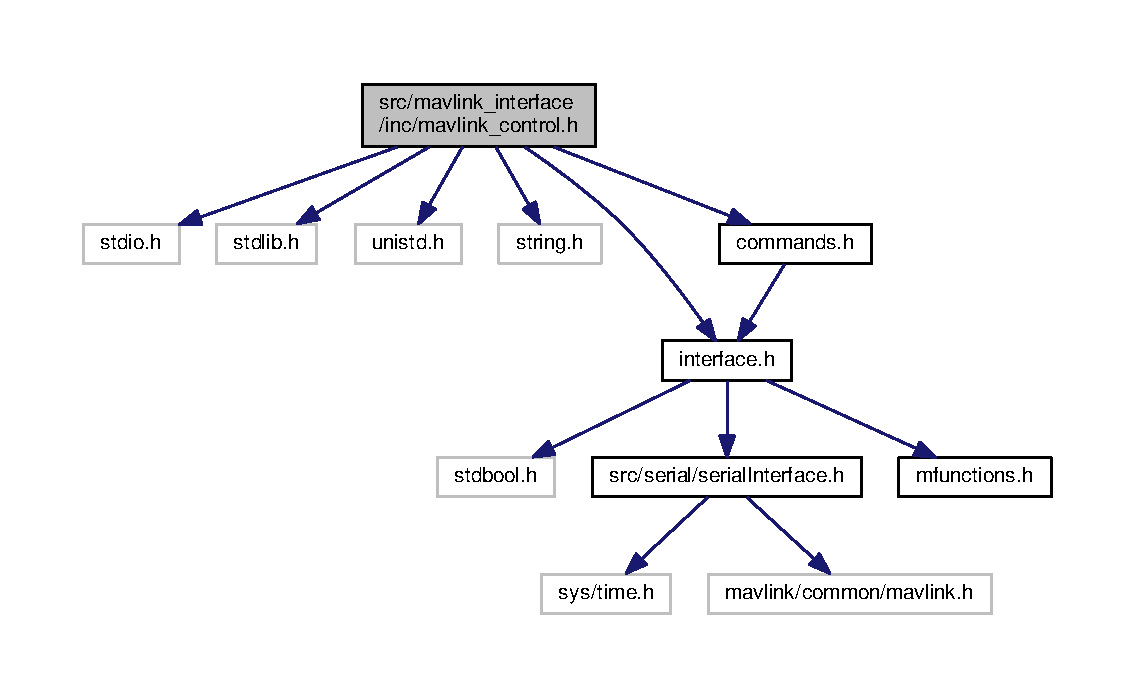
\includegraphics[width=350pt]{mavlink__control_8h__incl}
\end{center}
\end{figure}

\hypertarget{mfunctions_8h}{}\section{src/mavlink\+\_\+interface/inc/mfunctions.h File Reference}
\label{mfunctions_8h}\index{src/mavlink\+\_\+interface/inc/mfunctions.\+h@{src/mavlink\+\_\+interface/inc/mfunctions.\+h}}
This graph shows which files directly or indirectly include this file\+:
\nopagebreak
\begin{figure}[H]
\begin{center}
\leavevmode
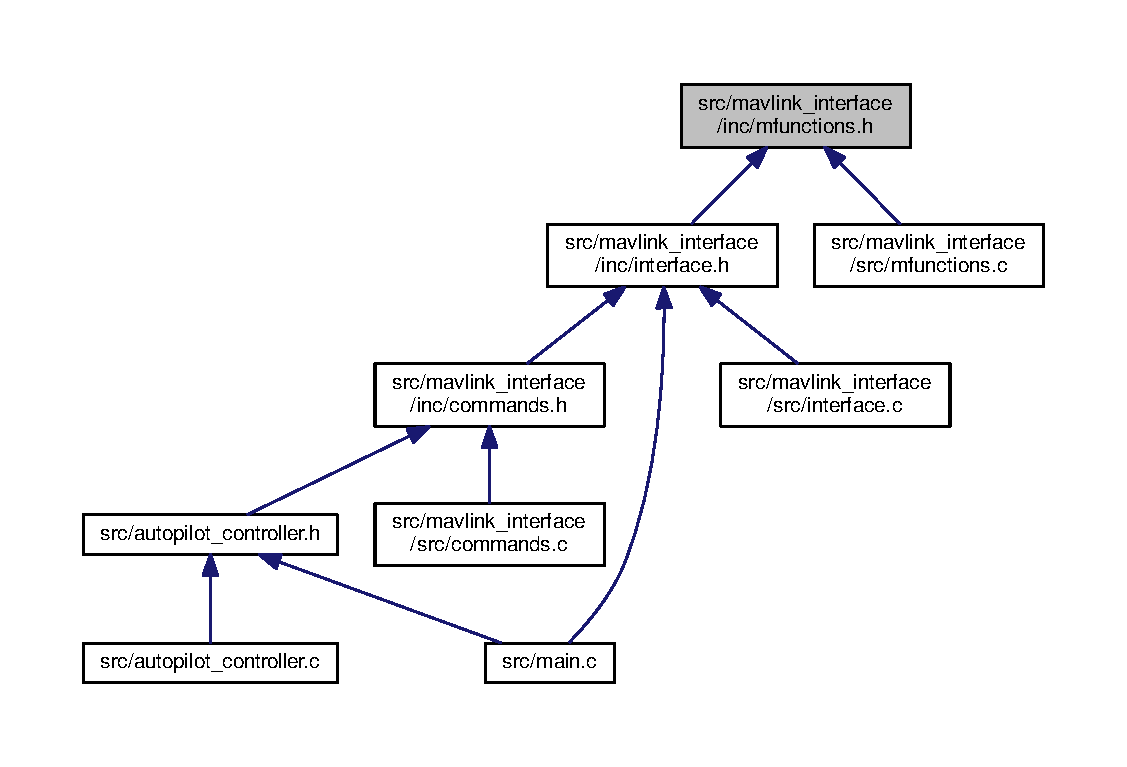
\includegraphics[width=350pt]{mfunctions_8h__dep__incl}
\end{center}
\end{figure}
\subsection*{Functions}
\begin{DoxyCompactItemize}
\item 
float \hyperlink{mfunctions_8h_a4e7ac5bb03cc548079cceaa888e45a8a}{tan\+\_\+2pi} (int angle)
\item 
float \hyperlink{mfunctions_8h_a71ab9e1f160bb0627b405c3b043434e6}{Beta} (int angle)
\end{DoxyCompactItemize}


\subsection{Function Documentation}
\index{mfunctions.\+h@{mfunctions.\+h}!Beta@{Beta}}
\index{Beta@{Beta}!mfunctions.\+h@{mfunctions.\+h}}
\subsubsection[{\texorpdfstring{Beta(int angle)}{Beta(int angle)}}]{\setlength{\rightskip}{0pt plus 5cm}float Beta (
\begin{DoxyParamCaption}
\item[{int}]{angle}
\end{DoxyParamCaption}
)}\hypertarget{mfunctions_8h_a71ab9e1f160bb0627b405c3b043434e6}{}\label{mfunctions_8h_a71ab9e1f160bb0627b405c3b043434e6}
\index{mfunctions.\+h@{mfunctions.\+h}!tan\+\_\+2pi@{tan\+\_\+2pi}}
\index{tan\+\_\+2pi@{tan\+\_\+2pi}!mfunctions.\+h@{mfunctions.\+h}}
\subsubsection[{\texorpdfstring{tan\+\_\+2pi(int angle)}{tan_2pi(int angle)}}]{\setlength{\rightskip}{0pt plus 5cm}float tan\+\_\+2pi (
\begin{DoxyParamCaption}
\item[{int}]{angle}
\end{DoxyParamCaption}
)}\hypertarget{mfunctions_8h_a4e7ac5bb03cc548079cceaa888e45a8a}{}\label{mfunctions_8h_a4e7ac5bb03cc548079cceaa888e45a8a}

\hypertarget{commands_8c}{}\section{src/mavlink\+\_\+interface/src/commands.c File Reference}
\label{commands_8c}\index{src/mavlink\+\_\+interface/src/commands.\+c@{src/mavlink\+\_\+interface/src/commands.\+c}}
{\ttfamily \#include $<$stdio.\+h$>$}\\*
{\ttfamily \#include $<$time.\+h$>$}\\*
{\ttfamily \#include $<$unistd.\+h$>$}\\*
{\ttfamily \#include \char`\"{}../inc/commands.\+h\char`\"{}}\\*
Include dependency graph for commands.\+c\+:
\nopagebreak
\begin{figure}[H]
\begin{center}
\leavevmode
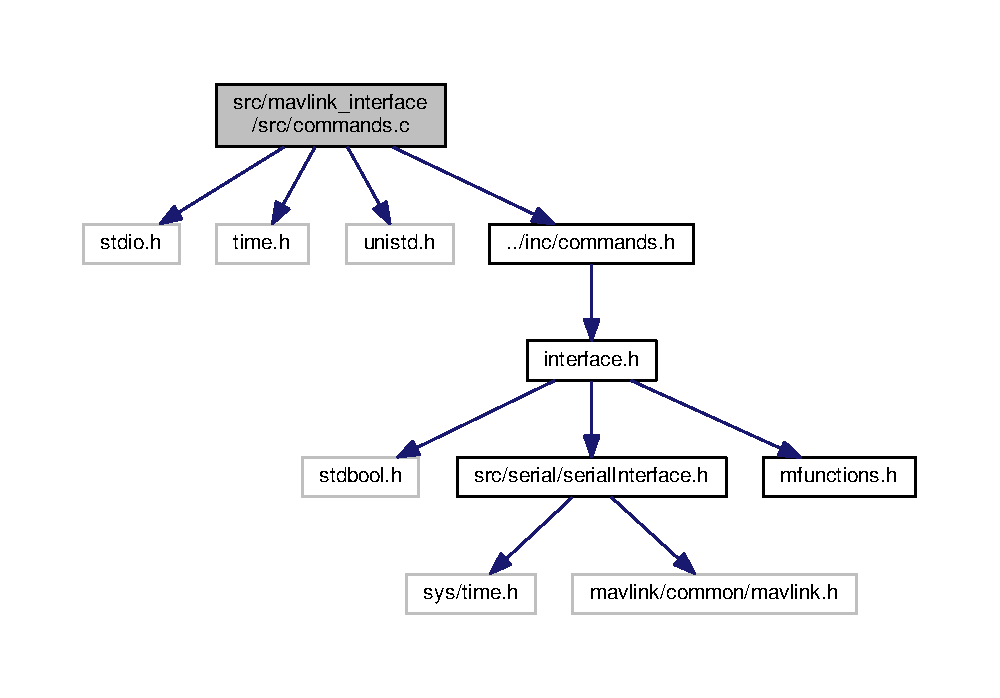
\includegraphics[width=350pt]{commands_8c__incl}
\end{center}
\end{figure}
\subsection*{Functions}
\begin{DoxyCompactItemize}
\item 
void \hyperlink{commands_8c_a03e9e7b262dbeae4cb8c4ae4a066531b}{operation} (float timer)
\item 
void \hyperlink{commands_8c_af36e37cab2a81a6258fcbcc6b8e28b29}{operation\+\_\+extended} (float timer)
\item 
void \hyperlink{commands_8c_a796cc160e31f24ab58c9826d316e5425}{square\+\_\+operation} (float timer)
\item 
void \hyperlink{commands_8c_a09b6928e3b393074a4435948174ae52b}{circle\+\_\+operation} (float timer)
\item 
void \hyperlink{commands_8c_aec823f3adf68cbb7a6fc0e022b85bf94}{automatic\+\_\+takeoff} (float timer, time\+\_\+t $\ast$begin)
\item 
void \hyperlink{commands_8c_a115b4a018fb4355a7f9c606b91faf9a4}{flight\+\_\+control\+\_\+sequence} (float timer)
\item 
void \hyperlink{commands_8c_a6abd769c5cbb26f123079227b2835497}{arm\+\_\+sequence} (void)
\item 
void \hyperlink{commands_8c_aa8ffb9b069939c32f2d4ae711bdca18f}{offboard\+\_\+control\+\_\+sequence} (void)
\item 
void \hyperlink{commands_8c_a0736eeabfa1f5ef6d6d5044e4e78898c}{disable\+\_\+offboard\+\_\+control\+\_\+sequence} (void)
\item 
void \hyperlink{commands_8c_a68b1b2487093eb85678440ab1629eeab}{disarm\+\_\+sequence} (void)
\item 
void \hyperlink{commands_8c_ad2d673badb605bcc66622ee8c7d7874b}{program\+\_\+counter\+\_\+sequence} (float timer, time\+\_\+t $\ast$begin)
\item 
void \hyperlink{commands_8c_a3c34d60eec74a2a54aaed0ee90a2178c}{autopilot\+\_\+write\+\_\+helper} (void)
\end{DoxyCompactItemize}
\subsection*{Variables}
\begin{DoxyCompactItemize}
\item 
int \hyperlink{commands_8c_ac5297d062c9a202719f7c02d6db58f3f}{arm\+\_\+lock} = 0
\item 
int \hyperlink{commands_8c_ace0573962d50abbb95e5aa6fb72d41ad}{offboard\+\_\+control\+\_\+lock} = 0
\item 
int \hyperlink{commands_8c_a37aa62835eedd0b028c96832a11800dd}{value\+\_\+mg\+\_\+x}
\item 
int \hyperlink{commands_8c_a200e61abaacec9ef9bf5ddb48e0f902f}{value\+\_\+mg\+\_\+y}
\item 
int \hyperlink{commands_8c_a3fbbac1ea7b32d7ccd2579de33e83c5e}{value\+\_\+mg\+\_\+z}
\item 
\hyperlink{types_8h_af6a258d8f3ee5206d682d799316314b1}{bool} \hyperlink{commands_8c_a27eb1c9f82b0b57dd66042fecbdb9cc4}{lock\+\_\+} = \hyperlink{types_8h_af6a258d8f3ee5206d682d799316314b1ae9de385ef6fe9bf3360d1038396b884c}{false}
\item 
int \hyperlink{commands_8c_a74c75d6d46b1bfa8d5dea82a38506f3a}{Program\+\_\+counter} = 0
\item 
volatile float \hyperlink{commands_8c_a6238cddccea71aca0723a82b1411dff6}{seconds} = 0
\item 
volatile float \hyperlink{commands_8c_a46bc98d6af5a6aaec9ca1365495a2b34}{omega} = 0
\item 
time\+\_\+t \hyperlink{commands_8c_a13455ba845bf5d4dba37be491bc6a036}{end}
\end{DoxyCompactItemize}


\subsection{Function Documentation}
\index{commands.\+c@{commands.\+c}!arm\+\_\+sequence@{arm\+\_\+sequence}}
\index{arm\+\_\+sequence@{arm\+\_\+sequence}!commands.\+c@{commands.\+c}}
\subsubsection[{\texorpdfstring{arm\+\_\+sequence(void)}{arm_sequence(void)}}]{\setlength{\rightskip}{0pt plus 5cm}void arm\+\_\+sequence (
\begin{DoxyParamCaption}
\item[{void}]{}
\end{DoxyParamCaption}
)}\hypertarget{commands_8c_a6abd769c5cbb26f123079227b2835497}{}\label{commands_8c_a6abd769c5cbb26f123079227b2835497}
\index{commands.\+c@{commands.\+c}!automatic\+\_\+takeoff@{automatic\+\_\+takeoff}}
\index{automatic\+\_\+takeoff@{automatic\+\_\+takeoff}!commands.\+c@{commands.\+c}}
\subsubsection[{\texorpdfstring{automatic\+\_\+takeoff(float timer, time\+\_\+t $\ast$begin)}{automatic_takeoff(float timer, time_t *begin)}}]{\setlength{\rightskip}{0pt plus 5cm}void automatic\+\_\+takeoff (
\begin{DoxyParamCaption}
\item[{float}]{timer, }
\item[{time\+\_\+t $\ast$}]{begin}
\end{DoxyParamCaption}
)}\hypertarget{commands_8c_aec823f3adf68cbb7a6fc0e022b85bf94}{}\label{commands_8c_aec823f3adf68cbb7a6fc0e022b85bf94}
\index{commands.\+c@{commands.\+c}!autopilot\+\_\+write\+\_\+helper@{autopilot\+\_\+write\+\_\+helper}}
\index{autopilot\+\_\+write\+\_\+helper@{autopilot\+\_\+write\+\_\+helper}!commands.\+c@{commands.\+c}}
\subsubsection[{\texorpdfstring{autopilot\+\_\+write\+\_\+helper(void)}{autopilot_write_helper(void)}}]{\setlength{\rightskip}{0pt plus 5cm}void autopilot\+\_\+write\+\_\+helper (
\begin{DoxyParamCaption}
\item[{void}]{}
\end{DoxyParamCaption}
)}\hypertarget{commands_8c_a3c34d60eec74a2a54aaed0ee90a2178c}{}\label{commands_8c_a3c34d60eec74a2a54aaed0ee90a2178c}
\index{commands.\+c@{commands.\+c}!circle\+\_\+operation@{circle\+\_\+operation}}
\index{circle\+\_\+operation@{circle\+\_\+operation}!commands.\+c@{commands.\+c}}
\subsubsection[{\texorpdfstring{circle\+\_\+operation(float timer)}{circle_operation(float timer)}}]{\setlength{\rightskip}{0pt plus 5cm}void circle\+\_\+operation (
\begin{DoxyParamCaption}
\item[{float}]{timer}
\end{DoxyParamCaption}
)}\hypertarget{commands_8c_a09b6928e3b393074a4435948174ae52b}{}\label{commands_8c_a09b6928e3b393074a4435948174ae52b}
\index{commands.\+c@{commands.\+c}!disable\+\_\+offboard\+\_\+control\+\_\+sequence@{disable\+\_\+offboard\+\_\+control\+\_\+sequence}}
\index{disable\+\_\+offboard\+\_\+control\+\_\+sequence@{disable\+\_\+offboard\+\_\+control\+\_\+sequence}!commands.\+c@{commands.\+c}}
\subsubsection[{\texorpdfstring{disable\+\_\+offboard\+\_\+control\+\_\+sequence(void)}{disable_offboard_control_sequence(void)}}]{\setlength{\rightskip}{0pt plus 5cm}void disable\+\_\+offboard\+\_\+control\+\_\+sequence (
\begin{DoxyParamCaption}
\item[{void}]{}
\end{DoxyParamCaption}
)}\hypertarget{commands_8c_a0736eeabfa1f5ef6d6d5044e4e78898c}{}\label{commands_8c_a0736eeabfa1f5ef6d6d5044e4e78898c}
\index{commands.\+c@{commands.\+c}!disarm\+\_\+sequence@{disarm\+\_\+sequence}}
\index{disarm\+\_\+sequence@{disarm\+\_\+sequence}!commands.\+c@{commands.\+c}}
\subsubsection[{\texorpdfstring{disarm\+\_\+sequence(void)}{disarm_sequence(void)}}]{\setlength{\rightskip}{0pt plus 5cm}void disarm\+\_\+sequence (
\begin{DoxyParamCaption}
\item[{void}]{}
\end{DoxyParamCaption}
)}\hypertarget{commands_8c_a68b1b2487093eb85678440ab1629eeab}{}\label{commands_8c_a68b1b2487093eb85678440ab1629eeab}
\index{commands.\+c@{commands.\+c}!flight\+\_\+control\+\_\+sequence@{flight\+\_\+control\+\_\+sequence}}
\index{flight\+\_\+control\+\_\+sequence@{flight\+\_\+control\+\_\+sequence}!commands.\+c@{commands.\+c}}
\subsubsection[{\texorpdfstring{flight\+\_\+control\+\_\+sequence(float timer)}{flight_control_sequence(float timer)}}]{\setlength{\rightskip}{0pt plus 5cm}void flight\+\_\+control\+\_\+sequence (
\begin{DoxyParamCaption}
\item[{float}]{timer}
\end{DoxyParamCaption}
)}\hypertarget{commands_8c_a115b4a018fb4355a7f9c606b91faf9a4}{}\label{commands_8c_a115b4a018fb4355a7f9c606b91faf9a4}
\index{commands.\+c@{commands.\+c}!offboard\+\_\+control\+\_\+sequence@{offboard\+\_\+control\+\_\+sequence}}
\index{offboard\+\_\+control\+\_\+sequence@{offboard\+\_\+control\+\_\+sequence}!commands.\+c@{commands.\+c}}
\subsubsection[{\texorpdfstring{offboard\+\_\+control\+\_\+sequence(void)}{offboard_control_sequence(void)}}]{\setlength{\rightskip}{0pt plus 5cm}void offboard\+\_\+control\+\_\+sequence (
\begin{DoxyParamCaption}
\item[{void}]{}
\end{DoxyParamCaption}
)}\hypertarget{commands_8c_aa8ffb9b069939c32f2d4ae711bdca18f}{}\label{commands_8c_aa8ffb9b069939c32f2d4ae711bdca18f}
\index{commands.\+c@{commands.\+c}!operation@{operation}}
\index{operation@{operation}!commands.\+c@{commands.\+c}}
\subsubsection[{\texorpdfstring{operation(float timer)}{operation(float timer)}}]{\setlength{\rightskip}{0pt plus 5cm}void operation (
\begin{DoxyParamCaption}
\item[{float}]{timer}
\end{DoxyParamCaption}
)}\hypertarget{commands_8c_a03e9e7b262dbeae4cb8c4ae4a066531b}{}\label{commands_8c_a03e9e7b262dbeae4cb8c4ae4a066531b}
\index{commands.\+c@{commands.\+c}!operation\+\_\+extended@{operation\+\_\+extended}}
\index{operation\+\_\+extended@{operation\+\_\+extended}!commands.\+c@{commands.\+c}}
\subsubsection[{\texorpdfstring{operation\+\_\+extended(float timer)}{operation_extended(float timer)}}]{\setlength{\rightskip}{0pt plus 5cm}void operation\+\_\+extended (
\begin{DoxyParamCaption}
\item[{float}]{timer}
\end{DoxyParamCaption}
)}\hypertarget{commands_8c_af36e37cab2a81a6258fcbcc6b8e28b29}{}\label{commands_8c_af36e37cab2a81a6258fcbcc6b8e28b29}
\index{commands.\+c@{commands.\+c}!program\+\_\+counter\+\_\+sequence@{program\+\_\+counter\+\_\+sequence}}
\index{program\+\_\+counter\+\_\+sequence@{program\+\_\+counter\+\_\+sequence}!commands.\+c@{commands.\+c}}
\subsubsection[{\texorpdfstring{program\+\_\+counter\+\_\+sequence(float timer, time\+\_\+t $\ast$begin)}{program_counter_sequence(float timer, time_t *begin)}}]{\setlength{\rightskip}{0pt plus 5cm}void program\+\_\+counter\+\_\+sequence (
\begin{DoxyParamCaption}
\item[{float}]{timer, }
\item[{time\+\_\+t $\ast$}]{begin}
\end{DoxyParamCaption}
)}\hypertarget{commands_8c_ad2d673badb605bcc66622ee8c7d7874b}{}\label{commands_8c_ad2d673badb605bcc66622ee8c7d7874b}
\index{commands.\+c@{commands.\+c}!square\+\_\+operation@{square\+\_\+operation}}
\index{square\+\_\+operation@{square\+\_\+operation}!commands.\+c@{commands.\+c}}
\subsubsection[{\texorpdfstring{square\+\_\+operation(float timer)}{square_operation(float timer)}}]{\setlength{\rightskip}{0pt plus 5cm}void square\+\_\+operation (
\begin{DoxyParamCaption}
\item[{float}]{timer}
\end{DoxyParamCaption}
)}\hypertarget{commands_8c_a796cc160e31f24ab58c9826d316e5425}{}\label{commands_8c_a796cc160e31f24ab58c9826d316e5425}


\subsection{Variable Documentation}
\index{commands.\+c@{commands.\+c}!arm\+\_\+lock@{arm\+\_\+lock}}
\index{arm\+\_\+lock@{arm\+\_\+lock}!commands.\+c@{commands.\+c}}
\subsubsection[{\texorpdfstring{arm\+\_\+lock}{arm_lock}}]{\setlength{\rightskip}{0pt plus 5cm}int arm\+\_\+lock = 0}\hypertarget{commands_8c_ac5297d062c9a202719f7c02d6db58f3f}{}\label{commands_8c_ac5297d062c9a202719f7c02d6db58f3f}
\index{commands.\+c@{commands.\+c}!end@{end}}
\index{end@{end}!commands.\+c@{commands.\+c}}
\subsubsection[{\texorpdfstring{end}{end}}]{\setlength{\rightskip}{0pt plus 5cm}time\+\_\+t end}\hypertarget{commands_8c_a13455ba845bf5d4dba37be491bc6a036}{}\label{commands_8c_a13455ba845bf5d4dba37be491bc6a036}
\index{commands.\+c@{commands.\+c}!lock\+\_\+@{lock\+\_\+}}
\index{lock\+\_\+@{lock\+\_\+}!commands.\+c@{commands.\+c}}
\subsubsection[{\texorpdfstring{lock\+\_\+}{lock_}}]{\setlength{\rightskip}{0pt plus 5cm}{\bf bool} lock\+\_\+ = {\bf false}}\hypertarget{commands_8c_a27eb1c9f82b0b57dd66042fecbdb9cc4}{}\label{commands_8c_a27eb1c9f82b0b57dd66042fecbdb9cc4}
\index{commands.\+c@{commands.\+c}!offboard\+\_\+control\+\_\+lock@{offboard\+\_\+control\+\_\+lock}}
\index{offboard\+\_\+control\+\_\+lock@{offboard\+\_\+control\+\_\+lock}!commands.\+c@{commands.\+c}}
\subsubsection[{\texorpdfstring{offboard\+\_\+control\+\_\+lock}{offboard_control_lock}}]{\setlength{\rightskip}{0pt plus 5cm}int offboard\+\_\+control\+\_\+lock = 0}\hypertarget{commands_8c_ace0573962d50abbb95e5aa6fb72d41ad}{}\label{commands_8c_ace0573962d50abbb95e5aa6fb72d41ad}
\index{commands.\+c@{commands.\+c}!omega@{omega}}
\index{omega@{omega}!commands.\+c@{commands.\+c}}
\subsubsection[{\texorpdfstring{omega}{omega}}]{\setlength{\rightskip}{0pt plus 5cm}volatile float omega = 0}\hypertarget{commands_8c_a46bc98d6af5a6aaec9ca1365495a2b34}{}\label{commands_8c_a46bc98d6af5a6aaec9ca1365495a2b34}
\index{commands.\+c@{commands.\+c}!Program\+\_\+counter@{Program\+\_\+counter}}
\index{Program\+\_\+counter@{Program\+\_\+counter}!commands.\+c@{commands.\+c}}
\subsubsection[{\texorpdfstring{Program\+\_\+counter}{Program_counter}}]{\setlength{\rightskip}{0pt plus 5cm}int Program\+\_\+counter = 0}\hypertarget{commands_8c_a74c75d6d46b1bfa8d5dea82a38506f3a}{}\label{commands_8c_a74c75d6d46b1bfa8d5dea82a38506f3a}
\index{commands.\+c@{commands.\+c}!seconds@{seconds}}
\index{seconds@{seconds}!commands.\+c@{commands.\+c}}
\subsubsection[{\texorpdfstring{seconds}{seconds}}]{\setlength{\rightskip}{0pt plus 5cm}volatile float seconds = 0}\hypertarget{commands_8c_a6238cddccea71aca0723a82b1411dff6}{}\label{commands_8c_a6238cddccea71aca0723a82b1411dff6}
\index{commands.\+c@{commands.\+c}!value\+\_\+mg\+\_\+x@{value\+\_\+mg\+\_\+x}}
\index{value\+\_\+mg\+\_\+x@{value\+\_\+mg\+\_\+x}!commands.\+c@{commands.\+c}}
\subsubsection[{\texorpdfstring{value\+\_\+mg\+\_\+x}{value_mg_x}}]{\setlength{\rightskip}{0pt plus 5cm}int value\+\_\+mg\+\_\+x}\hypertarget{commands_8c_a37aa62835eedd0b028c96832a11800dd}{}\label{commands_8c_a37aa62835eedd0b028c96832a11800dd}
\index{commands.\+c@{commands.\+c}!value\+\_\+mg\+\_\+y@{value\+\_\+mg\+\_\+y}}
\index{value\+\_\+mg\+\_\+y@{value\+\_\+mg\+\_\+y}!commands.\+c@{commands.\+c}}
\subsubsection[{\texorpdfstring{value\+\_\+mg\+\_\+y}{value_mg_y}}]{\setlength{\rightskip}{0pt plus 5cm}int value\+\_\+mg\+\_\+y}\hypertarget{commands_8c_a200e61abaacec9ef9bf5ddb48e0f902f}{}\label{commands_8c_a200e61abaacec9ef9bf5ddb48e0f902f}
\index{commands.\+c@{commands.\+c}!value\+\_\+mg\+\_\+z@{value\+\_\+mg\+\_\+z}}
\index{value\+\_\+mg\+\_\+z@{value\+\_\+mg\+\_\+z}!commands.\+c@{commands.\+c}}
\subsubsection[{\texorpdfstring{value\+\_\+mg\+\_\+z}{value_mg_z}}]{\setlength{\rightskip}{0pt plus 5cm}int value\+\_\+mg\+\_\+z}\hypertarget{commands_8c_a3fbbac1ea7b32d7ccd2579de33e83c5e}{}\label{commands_8c_a3fbbac1ea7b32d7ccd2579de33e83c5e}

\hypertarget{commands_8d}{}\section{src/mavlink\+\_\+interface/src/commands.d File Reference}
\label{commands_8d}\index{src/mavlink\+\_\+interface/src/commands.\+d@{src/mavlink\+\_\+interface/src/commands.\+d}}

\hypertarget{interface_8c}{}\section{src/mavlink\+\_\+interface/src/interface.c File Reference}
\label{interface_8c}\index{src/mavlink\+\_\+interface/src/interface.\+c@{src/mavlink\+\_\+interface/src/interface.\+c}}
{\ttfamily \#include $<$stdio.\+h$>$}\\*
{\ttfamily \#include \char`\"{}../inc/interface.\+h\char`\"{}}\\*
Include dependency graph for interface.\+c\+:\nopagebreak
\begin{figure}[H]
\begin{center}
\leavevmode
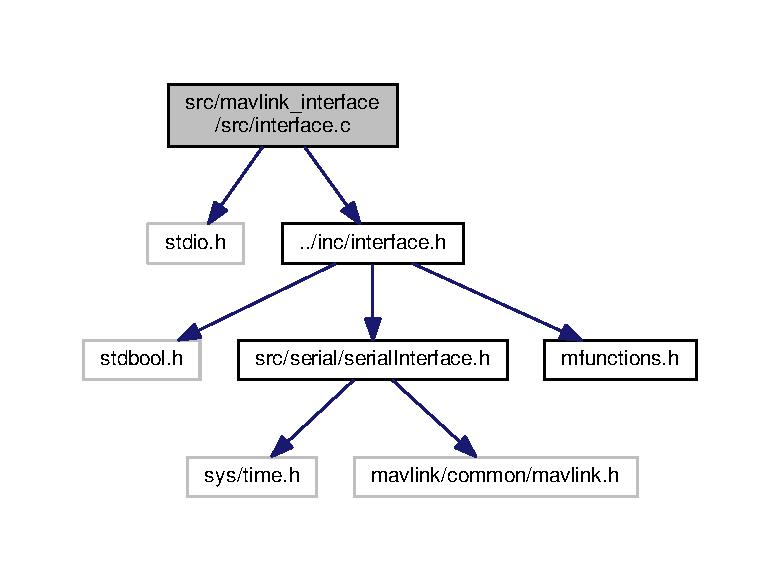
\includegraphics[width=350pt]{interface_8c__incl}
\end{center}
\end{figure}
\subsection*{Functions}
\begin{DoxyCompactItemize}
\item 
\hyperlink{struct_time___stamps}{Time\+\_\+\+Stamps} \hyperlink{interface_8c_a826db1ee378517996e36fba7482cb29b}{create\+\_\+\+Time\+Stamps} ()
\item 
void \hyperlink{interface_8c_a49dac88e99881e75459b0bc15354378b}{reset\+\_\+timestamps} (\hyperlink{struct_time___stamps}{Time\+\_\+\+Stamps} $\ast$time\+\_\+stamps)
\begin{DoxyCompactList}\small\item\em Zeros out all the timestamps. \end{DoxyCompactList}\item 
void \hyperlink{interface_8c_aa4bd4ad9917c2577168def15cf9aefb7}{autopilot\+\_\+initialize} (void)
\begin{DoxyCompactList}\small\item\em Initialize system-\/wide important parameters and flags. \end{DoxyCompactList}\item 
void \hyperlink{interface_8c_aeeb66c18def4c2bb8c404a75ccf4ff07}{autopilot\+\_\+start} (void)
\begin{DoxyCompactList}\small\item\em Used to define the initial position. This method is supposed to be called once on startup after the first call to read\+\_\+message() (which listens for a position message from the autopilot). \end{DoxyCompactList}\item 
void \hyperlink{interface_8c_a761018fc7556aac6d6f302b7406f791d}{read\+\_\+messages} (void)
\begin{DoxyCompactList}\small\item\em Reads M\+A\+V\+Link messages from the autopilot until all requested messages are received (this is controlled by the received\+\_\+all flag inside the function). The received messages are set in the \hyperlink{struct_mavlink___messages}{Mavlink\+\_\+\+Messages}. This method is blocking and will not exit until all requested messages are obtained (may become an infinite loop). \end{DoxyCompactList}\item 
void \hyperlink{interface_8c_aa400b6caf4a262ea4446854e90ab005d}{autopilot\+\_\+write} (void)
\begin{DoxyCompactList}\small\item\em A \char`\"{}dummy\char`\"{} method that writes a void (all zeros) setpoint to the autopilot. Used to signal startup. \end{DoxyCompactList}\item 
void \hyperlink{interface_8c_ab2559012cba7e4c72ec10a59c87f84cb}{autopilot\+\_\+write\+\_\+setpoint} (void)
\begin{DoxyCompactList}\small\item\em Write the current setpoint to the autopilot after it\textquotesingle{}s been updated (needs to be called explicitly) \end{DoxyCompactList}\item 
void \hyperlink{interface_8c_ac8fa807910345b796fe4fd9f61101ba2}{autopilot\+\_\+write\+\_\+message} (mavlink\+\_\+message\+\_\+t message)
\begin{DoxyCompactList}\small\item\em Write a M\+A\+V\+Link message to the autopilot. \end{DoxyCompactList}\item 
void \hyperlink{interface_8c_a7a3598bf63d9844fcd22328fc63842a4}{autopilot\+\_\+update\+\_\+setpoint} (mavlink\+\_\+set\+\_\+position\+\_\+target\+\_\+local\+\_\+ned\+\_\+t setpoint)
\begin{DoxyCompactList}\small\item\em Update the current setpoint with the given setpoint. \end{DoxyCompactList}\item 
\hyperlink{types_8h_af6a258d8f3ee5206d682d799316314b1}{bool} \hyperlink{interface_8c_a6f0b501cf0b9b1e74c0053df49b3bdc6}{enable\+\_\+offboard\+\_\+control} (void)
\begin{DoxyCompactList}\small\item\em Enables the offboard control of the autopilot, setting the appropriate flag. \end{DoxyCompactList}\item 
\hyperlink{types_8h_af6a258d8f3ee5206d682d799316314b1}{bool} \hyperlink{interface_8c_a4b3151ecef548d647281eba568170280}{disable\+\_\+offboard\+\_\+control} (void)
\begin{DoxyCompactList}\small\item\em Disabled the offboard control of the autopilot. \end{DoxyCompactList}\item 
int \hyperlink{interface_8c_a22fb091245542a81979c3d517c048d9c}{toggle\+\_\+offboard\+\_\+control} (\hyperlink{types_8h_af6a258d8f3ee5206d682d799316314b1}{bool} flag)
\begin{DoxyCompactList}\small\item\em The function that\textquotesingle{}s used by enable/disable\+\_\+offbard\+\_\+control() to actually write the appropriate command to the autopilot. \end{DoxyCompactList}\item 
void \hyperlink{interface_8c_ae4ffa041a7021553ce57bcc004721afe}{autopilot\+\_\+arm} (void)
\begin{DoxyCompactList}\small\item\em Arm the autopilot. \end{DoxyCompactList}\item 
void \hyperlink{interface_8c_ab784fd6af4d00965889893c0cf462f26}{autopilot\+\_\+disarm} (void)
\begin{DoxyCompactList}\small\item\em Disarm the autopilot. \end{DoxyCompactList}\item 
int \hyperlink{interface_8c_ae2645ae25eb4ac098eb579dd9a49c1b9}{toggle\+\_\+arm\+\_\+disarm} (\hyperlink{types_8h_af6a258d8f3ee5206d682d799316314b1}{bool} flag)
\begin{DoxyCompactList}\small\item\em Used by autopilot\+\_\+arm/disarm() in a similar manner to toogle\+\_\+offboard\+\_\+control(). \end{DoxyCompactList}\item 
int \hyperlink{interface_8c_a56a6826eb5bf8127144d09ecfa6bee9a}{check\+\_\+offboard\+\_\+control} (void)
\begin{DoxyCompactList}\small\item\em A convenience function to check if the autopilot is in offboard control or not. \end{DoxyCompactList}\item 
int \hyperlink{interface_8c_a8140deb719d9d4350a97d225d1d2cd04}{check\+\_\+arm\+\_\+disarm} (void)
\begin{DoxyCompactList}\small\item\em Similar to \hyperlink{interface_8h_a56a6826eb5bf8127144d09ecfa6bee9a}{check\+\_\+offboard\+\_\+control()}. \end{DoxyCompactList}\item 
int \hyperlink{interface_8c_a778200ebd979982133bd3965e49976a5}{check\+\_\+message} (uint16\+\_\+t C\+O\+M\+M\+A\+N\+D\+\_\+\+ID)
\begin{DoxyCompactList}\small\item\em The function that\textquotesingle{}s used by \hyperlink{interface_8h_a56a6826eb5bf8127144d09ecfa6bee9a}{check\+\_\+offboard\+\_\+control()} and \hyperlink{interface_8h_a8140deb719d9d4350a97d225d1d2cd04}{check\+\_\+arm\+\_\+disarm()} to determine the status. \end{DoxyCompactList}\item 
void \hyperlink{interface_8c_a9e40ef161fe282aa0ca0cb9a436f56e8}{set\+\_\+position} (float x, float y, float z, mavlink\+\_\+set\+\_\+position\+\_\+target\+\_\+local\+\_\+ned\+\_\+t $\ast$set\+\_\+position)
\item 
void \hyperlink{interface_8c_a7e830228a3f61cead91708a03b562c0f}{set\+\_\+velocity} (float vx, float vy, float vz, mavlink\+\_\+set\+\_\+position\+\_\+target\+\_\+local\+\_\+ned\+\_\+t $\ast$sp)
\item 
void \hyperlink{interface_8c_ad089b2003c05af61daf45a455dba3c65}{set\+\_\+yaw} (float yaw, mavlink\+\_\+set\+\_\+position\+\_\+target\+\_\+local\+\_\+ned\+\_\+t $\ast$sp)
\item 
void \hyperlink{interface_8c_ae8a0b0240696473ecad32978283824b8}{set\+\_\+\+\_\+} (float x, float y, float z, mavlink\+\_\+set\+\_\+position\+\_\+target\+\_\+local\+\_\+ned\+\_\+t $\ast$final\+\_\+set\+\_\+point)
\item 
void \hyperlink{interface_8c_aaf2bde2dc6e6e3ea59ddd5e36549f3ab}{position\+\_\+and\+\_\+speed\+\_\+set} (float x, float y, float z, float vx, float vy, float vz, mavlink\+\_\+set\+\_\+position\+\_\+target\+\_\+local\+\_\+ned\+\_\+t $\ast$final\+\_\+set\+\_\+point)
\item 
void \hyperlink{interface_8c_a66e1f11d723feacc42bbca4020f3a858}{set\+\_\+circle} (float R, float theta, float z, mavlink\+\_\+set\+\_\+position\+\_\+target\+\_\+local\+\_\+ned\+\_\+t $\ast$set\+\_\+point)
\item 
uint64\+\_\+t \hyperlink{interface_8c_a2ac9437af95602ce4e5ba39be2d2429b}{get\+\_\+time\+\_\+usec} (void)
\end{DoxyCompactItemize}
\subsection*{Variables}
\begin{DoxyCompactItemize}
\item 
char \hyperlink{interface_8c_a81859badc92ff83adb55fa6730145cf3}{control\+\_\+status}
\item 
char \hyperlink{interface_8c_ac3c75d0f6f80c41ac1b5453695114156}{arm\+\_\+status}
\item 
int \hyperlink{interface_8c_a21626f3691ef6b48b44970d7f3cb5964}{system\+\_\+id}
\item 
int \hyperlink{interface_8c_abdd15bddb613a8f681f606249dc4f1b0}{autopilot\+\_\+id}
\item 
int \hyperlink{interface_8c_a3bfded90b2b7d45e0da89c99f1e7bdfb}{companion\+\_\+id}
\item 
\hyperlink{struct_mavlink___messages}{Mavlink\+\_\+\+Messages} \hyperlink{interface_8c_ab305999d6776734f996598fc8b065d5d}{current\+\_\+messages}
\item 
mavlink\+\_\+set\+\_\+position\+\_\+target\+\_\+local\+\_\+ned\+\_\+t \hyperlink{interface_8c_a6fc9a01a226e2fa8f86ac3c3f7569741}{current\+\_\+setpoint}
\item 
mavlink\+\_\+set\+\_\+position\+\_\+target\+\_\+local\+\_\+ned\+\_\+t \hyperlink{interface_8c_a72a68d2d5fb3d88b82654a2d68377bfb}{initial\+\_\+position}
\item 
mavlink\+\_\+set\+\_\+position\+\_\+target\+\_\+local\+\_\+ned\+\_\+t \hyperlink{interface_8c_af5687cd9ba18c55c0fbe8e7d346ad8be}{ip}
\item 
int \hyperlink{interface_8c_a6000f659d29885840bc5462292885c7d}{initial\+\_\+position\+\_\+lock} = 0
\item 
float \hyperlink{interface_8c_aa5450ccd24b24476021f95ad4af371ec}{highres\+\_\+flag} = 1
\item 
int \hyperlink{interface_8c_ac9cad88b398a367f0e13ec5622eceaa3}{lock\+\_\+read\+\_\+messages} = 0
\end{DoxyCompactItemize}


\subsection{Function Documentation}
\index{interface.\+c@{interface.\+c}!autopilot\+\_\+arm@{autopilot\+\_\+arm}}
\index{autopilot\+\_\+arm@{autopilot\+\_\+arm}!interface.\+c@{interface.\+c}}
\subsubsection[{\texorpdfstring{autopilot\+\_\+arm(void)}{autopilot_arm(void)}}]{\setlength{\rightskip}{0pt plus 5cm}void autopilot\+\_\+arm (
\begin{DoxyParamCaption}
\item[{void}]{}
\end{DoxyParamCaption}
)}\hypertarget{interface_8c_ae4ffa041a7021553ce57bcc004721afe}{}\label{interface_8c_ae4ffa041a7021553ce57bcc004721afe}


Arm the autopilot. 

\index{interface.\+c@{interface.\+c}!autopilot\+\_\+disarm@{autopilot\+\_\+disarm}}
\index{autopilot\+\_\+disarm@{autopilot\+\_\+disarm}!interface.\+c@{interface.\+c}}
\subsubsection[{\texorpdfstring{autopilot\+\_\+disarm(void)}{autopilot_disarm(void)}}]{\setlength{\rightskip}{0pt plus 5cm}void autopilot\+\_\+disarm (
\begin{DoxyParamCaption}
\item[{void}]{}
\end{DoxyParamCaption}
)}\hypertarget{interface_8c_ab784fd6af4d00965889893c0cf462f26}{}\label{interface_8c_ab784fd6af4d00965889893c0cf462f26}


Disarm the autopilot. 

\index{interface.\+c@{interface.\+c}!autopilot\+\_\+initialize@{autopilot\+\_\+initialize}}
\index{autopilot\+\_\+initialize@{autopilot\+\_\+initialize}!interface.\+c@{interface.\+c}}
\subsubsection[{\texorpdfstring{autopilot\+\_\+initialize(void)}{autopilot_initialize(void)}}]{\setlength{\rightskip}{0pt plus 5cm}void autopilot\+\_\+initialize (
\begin{DoxyParamCaption}
\item[{void}]{}
\end{DoxyParamCaption}
)}\hypertarget{interface_8c_aa4bd4ad9917c2577168def15cf9aefb7}{}\label{interface_8c_aa4bd4ad9917c2577168def15cf9aefb7}


Initialize system-\/wide important parameters and flags. 

\index{interface.\+c@{interface.\+c}!autopilot\+\_\+start@{autopilot\+\_\+start}}
\index{autopilot\+\_\+start@{autopilot\+\_\+start}!interface.\+c@{interface.\+c}}
\subsubsection[{\texorpdfstring{autopilot\+\_\+start(void)}{autopilot_start(void)}}]{\setlength{\rightskip}{0pt plus 5cm}void autopilot\+\_\+start (
\begin{DoxyParamCaption}
\item[{void}]{}
\end{DoxyParamCaption}
)}\hypertarget{interface_8c_aeeb66c18def4c2bb8c404a75ccf4ff07}{}\label{interface_8c_aeeb66c18def4c2bb8c404a75ccf4ff07}


Used to define the initial position. This method is supposed to be called once on startup after the first call to read\+\_\+message() (which listens for a position message from the autopilot). 

\index{interface.\+c@{interface.\+c}!autopilot\+\_\+update\+\_\+setpoint@{autopilot\+\_\+update\+\_\+setpoint}}
\index{autopilot\+\_\+update\+\_\+setpoint@{autopilot\+\_\+update\+\_\+setpoint}!interface.\+c@{interface.\+c}}
\subsubsection[{\texorpdfstring{autopilot\+\_\+update\+\_\+setpoint(mavlink\+\_\+set\+\_\+position\+\_\+target\+\_\+local\+\_\+ned\+\_\+t setpoint)}{autopilot_update_setpoint(mavlink_set_position_target_local_ned_t setpoint)}}]{\setlength{\rightskip}{0pt plus 5cm}void autopilot\+\_\+update\+\_\+setpoint (
\begin{DoxyParamCaption}
\item[{mavlink\+\_\+set\+\_\+position\+\_\+target\+\_\+local\+\_\+ned\+\_\+t}]{setpoint}
\end{DoxyParamCaption}
)}\hypertarget{interface_8c_a7a3598bf63d9844fcd22328fc63842a4}{}\label{interface_8c_a7a3598bf63d9844fcd22328fc63842a4}


Update the current setpoint with the given setpoint. 


\begin{DoxyParams}[1]{Parameters}
\mbox{\tt in}  & {\em setpoint} & A S\+E\+T\+\_\+\+P\+O\+S\+I\+T\+I\+O\+N\+\_\+\+L\+O\+C\+A\+L\+\_\+\+N\+ED struct that is assigned to the current setpoint. \\
\hline
\end{DoxyParams}
\index{interface.\+c@{interface.\+c}!autopilot\+\_\+write@{autopilot\+\_\+write}}
\index{autopilot\+\_\+write@{autopilot\+\_\+write}!interface.\+c@{interface.\+c}}
\subsubsection[{\texorpdfstring{autopilot\+\_\+write(void)}{autopilot_write(void)}}]{\setlength{\rightskip}{0pt plus 5cm}void autopilot\+\_\+write (
\begin{DoxyParamCaption}
\item[{void}]{}
\end{DoxyParamCaption}
)}\hypertarget{interface_8c_aa400b6caf4a262ea4446854e90ab005d}{}\label{interface_8c_aa400b6caf4a262ea4446854e90ab005d}


A \char`\"{}dummy\char`\"{} method that writes a void (all zeros) setpoint to the autopilot. Used to signal startup. 

\index{interface.\+c@{interface.\+c}!autopilot\+\_\+write\+\_\+message@{autopilot\+\_\+write\+\_\+message}}
\index{autopilot\+\_\+write\+\_\+message@{autopilot\+\_\+write\+\_\+message}!interface.\+c@{interface.\+c}}
\subsubsection[{\texorpdfstring{autopilot\+\_\+write\+\_\+message(mavlink\+\_\+message\+\_\+t message)}{autopilot_write_message(mavlink_message_t message)}}]{\setlength{\rightskip}{0pt plus 5cm}void autopilot\+\_\+write\+\_\+message (
\begin{DoxyParamCaption}
\item[{mavlink\+\_\+message\+\_\+t}]{message}
\end{DoxyParamCaption}
)}\hypertarget{interface_8c_ac8fa807910345b796fe4fd9f61101ba2}{}\label{interface_8c_ac8fa807910345b796fe4fd9f61101ba2}


Write a M\+A\+V\+Link message to the autopilot. 


\begin{DoxyParams}[1]{Parameters}
\mbox{\tt in}  & {\em message} & A M\+A\+V\+Link message struct with the encapsulated message \\
\hline
\end{DoxyParams}
\index{interface.\+c@{interface.\+c}!autopilot\+\_\+write\+\_\+setpoint@{autopilot\+\_\+write\+\_\+setpoint}}
\index{autopilot\+\_\+write\+\_\+setpoint@{autopilot\+\_\+write\+\_\+setpoint}!interface.\+c@{interface.\+c}}
\subsubsection[{\texorpdfstring{autopilot\+\_\+write\+\_\+setpoint(void)}{autopilot_write_setpoint(void)}}]{\setlength{\rightskip}{0pt plus 5cm}void autopilot\+\_\+write\+\_\+setpoint (
\begin{DoxyParamCaption}
\item[{void}]{}
\end{DoxyParamCaption}
)}\hypertarget{interface_8c_ab2559012cba7e4c72ec10a59c87f84cb}{}\label{interface_8c_ab2559012cba7e4c72ec10a59c87f84cb}


Write the current setpoint to the autopilot after it\textquotesingle{}s been updated (needs to be called explicitly) 

\index{interface.\+c@{interface.\+c}!check\+\_\+arm\+\_\+disarm@{check\+\_\+arm\+\_\+disarm}}
\index{check\+\_\+arm\+\_\+disarm@{check\+\_\+arm\+\_\+disarm}!interface.\+c@{interface.\+c}}
\subsubsection[{\texorpdfstring{check\+\_\+arm\+\_\+disarm(void)}{check_arm_disarm(void)}}]{\setlength{\rightskip}{0pt plus 5cm}int check\+\_\+arm\+\_\+disarm (
\begin{DoxyParamCaption}
\item[{void}]{}
\end{DoxyParamCaption}
)}\hypertarget{interface_8c_a8140deb719d9d4350a97d225d1d2cd04}{}\label{interface_8c_a8140deb719d9d4350a97d225d1d2cd04}


Similar to \hyperlink{interface_8h_a56a6826eb5bf8127144d09ecfa6bee9a}{check\+\_\+offboard\+\_\+control()}. 

\begin{DoxyReturn}{Returns}
true if armed and false if disarmed. 
\end{DoxyReturn}
\index{interface.\+c@{interface.\+c}!check\+\_\+message@{check\+\_\+message}}
\index{check\+\_\+message@{check\+\_\+message}!interface.\+c@{interface.\+c}}
\subsubsection[{\texorpdfstring{check\+\_\+message(uint16\+\_\+t C\+O\+M\+M\+A\+N\+D\+\_\+\+I\+D)}{check_message(uint16_t COMMAND_ID)}}]{\setlength{\rightskip}{0pt plus 5cm}int check\+\_\+message (
\begin{DoxyParamCaption}
\item[{uint16\+\_\+t}]{C\+O\+M\+M\+A\+N\+D\+\_\+\+ID}
\end{DoxyParamCaption}
)}\hypertarget{interface_8c_a778200ebd979982133bd3965e49976a5}{}\label{interface_8c_a778200ebd979982133bd3965e49976a5}


The function that\textquotesingle{}s used by \hyperlink{interface_8h_a56a6826eb5bf8127144d09ecfa6bee9a}{check\+\_\+offboard\+\_\+control()} and \hyperlink{interface_8h_a8140deb719d9d4350a97d225d1d2cd04}{check\+\_\+arm\+\_\+disarm()} to determine the status. 


\begin{DoxyParams}[1]{Parameters}
\mbox{\tt in}  & {\em C\+O\+M\+M\+A\+N\+D\+\_\+\+ID} & The ID of the command as defined by the M\+A\+V\+Link protocol.\\
\hline
\end{DoxyParams}
\begin{DoxyReturn}{Returns}
1 for a positive command\+\_\+ack. 0 otherwise. 
\end{DoxyReturn}
\index{interface.\+c@{interface.\+c}!check\+\_\+offboard\+\_\+control@{check\+\_\+offboard\+\_\+control}}
\index{check\+\_\+offboard\+\_\+control@{check\+\_\+offboard\+\_\+control}!interface.\+c@{interface.\+c}}
\subsubsection[{\texorpdfstring{check\+\_\+offboard\+\_\+control(void)}{check_offboard_control(void)}}]{\setlength{\rightskip}{0pt plus 5cm}int check\+\_\+offboard\+\_\+control (
\begin{DoxyParamCaption}
\item[{void}]{}
\end{DoxyParamCaption}
)}\hypertarget{interface_8c_a56a6826eb5bf8127144d09ecfa6bee9a}{}\label{interface_8c_a56a6826eb5bf8127144d09ecfa6bee9a}


A convenience function to check if the autopilot is in offboard control or not. 

\begin{DoxyReturn}{Returns}
true if the autopilot is under offboard control, false otherwise. 
\end{DoxyReturn}
\index{interface.\+c@{interface.\+c}!create\+\_\+\+Time\+Stamps@{create\+\_\+\+Time\+Stamps}}
\index{create\+\_\+\+Time\+Stamps@{create\+\_\+\+Time\+Stamps}!interface.\+c@{interface.\+c}}
\subsubsection[{\texorpdfstring{create\+\_\+\+Time\+Stamps()}{create_TimeStamps()}}]{\setlength{\rightskip}{0pt plus 5cm}{\bf Time\+\_\+\+Stamps} create\+\_\+\+Time\+Stamps (
\begin{DoxyParamCaption}
{}
\end{DoxyParamCaption}
)}\hypertarget{interface_8c_a826db1ee378517996e36fba7482cb29b}{}\label{interface_8c_a826db1ee378517996e36fba7482cb29b}
\index{interface.\+c@{interface.\+c}!disable\+\_\+offboard\+\_\+control@{disable\+\_\+offboard\+\_\+control}}
\index{disable\+\_\+offboard\+\_\+control@{disable\+\_\+offboard\+\_\+control}!interface.\+c@{interface.\+c}}
\subsubsection[{\texorpdfstring{disable\+\_\+offboard\+\_\+control(void)}{disable_offboard_control(void)}}]{\setlength{\rightskip}{0pt plus 5cm}{\bf bool} disable\+\_\+offboard\+\_\+control (
\begin{DoxyParamCaption}
\item[{void}]{}
\end{DoxyParamCaption}
)}\hypertarget{interface_8c_a4b3151ecef548d647281eba568170280}{}\label{interface_8c_a4b3151ecef548d647281eba568170280}


Disabled the offboard control of the autopilot. 

\begin{DoxyReturn}{Returns}
The offboard control status\+: true for active offboard control and false for disabled offboard control. 
\end{DoxyReturn}
\index{interface.\+c@{interface.\+c}!enable\+\_\+offboard\+\_\+control@{enable\+\_\+offboard\+\_\+control}}
\index{enable\+\_\+offboard\+\_\+control@{enable\+\_\+offboard\+\_\+control}!interface.\+c@{interface.\+c}}
\subsubsection[{\texorpdfstring{enable\+\_\+offboard\+\_\+control(void)}{enable_offboard_control(void)}}]{\setlength{\rightskip}{0pt plus 5cm}{\bf bool} enable\+\_\+offboard\+\_\+control (
\begin{DoxyParamCaption}
\item[{void}]{}
\end{DoxyParamCaption}
)}\hypertarget{interface_8c_a6f0b501cf0b9b1e74c0053df49b3bdc6}{}\label{interface_8c_a6f0b501cf0b9b1e74c0053df49b3bdc6}


Enables the offboard control of the autopilot, setting the appropriate flag. 

\begin{DoxyReturn}{Returns}
Similar to \hyperlink{interface_8h_a4b3151ecef548d647281eba568170280}{disable\+\_\+offboard\+\_\+control()} but the inverse (true for successfully enabling offboard control). 
\end{DoxyReturn}
\index{interface.\+c@{interface.\+c}!get\+\_\+time\+\_\+usec@{get\+\_\+time\+\_\+usec}}
\index{get\+\_\+time\+\_\+usec@{get\+\_\+time\+\_\+usec}!interface.\+c@{interface.\+c}}
\subsubsection[{\texorpdfstring{get\+\_\+time\+\_\+usec(void)}{get_time_usec(void)}}]{\setlength{\rightskip}{0pt plus 5cm}uint64\+\_\+t get\+\_\+time\+\_\+usec (
\begin{DoxyParamCaption}
\item[{void}]{}
\end{DoxyParamCaption}
)}\hypertarget{interface_8c_a2ac9437af95602ce4e5ba39be2d2429b}{}\label{interface_8c_a2ac9437af95602ce4e5ba39be2d2429b}
\index{interface.\+c@{interface.\+c}!position\+\_\+and\+\_\+speed\+\_\+set@{position\+\_\+and\+\_\+speed\+\_\+set}}
\index{position\+\_\+and\+\_\+speed\+\_\+set@{position\+\_\+and\+\_\+speed\+\_\+set}!interface.\+c@{interface.\+c}}
\subsubsection[{\texorpdfstring{position\+\_\+and\+\_\+speed\+\_\+set(float x, float y, float z, float vx, float vy, float vz, mavlink\+\_\+set\+\_\+position\+\_\+target\+\_\+local\+\_\+ned\+\_\+t $\ast$final\+\_\+set\+\_\+point)}{position_and_speed_set(float x, float y, float z, float vx, float vy, float vz, mavlink_set_position_target_local_ned_t *final_set_point)}}]{\setlength{\rightskip}{0pt plus 5cm}void position\+\_\+and\+\_\+speed\+\_\+set (
\begin{DoxyParamCaption}
\item[{float}]{x, }
\item[{float}]{y, }
\item[{float}]{z, }
\item[{float}]{vx, }
\item[{float}]{vy, }
\item[{float}]{vz, }
\item[{mavlink\+\_\+set\+\_\+position\+\_\+target\+\_\+local\+\_\+ned\+\_\+t $\ast$}]{final\+\_\+set\+\_\+point}
\end{DoxyParamCaption}
)}\hypertarget{interface_8c_aaf2bde2dc6e6e3ea59ddd5e36549f3ab}{}\label{interface_8c_aaf2bde2dc6e6e3ea59ddd5e36549f3ab}
\index{interface.\+c@{interface.\+c}!read\+\_\+messages@{read\+\_\+messages}}
\index{read\+\_\+messages@{read\+\_\+messages}!interface.\+c@{interface.\+c}}
\subsubsection[{\texorpdfstring{read\+\_\+messages(void)}{read_messages(void)}}]{\setlength{\rightskip}{0pt plus 5cm}void read\+\_\+messages (
\begin{DoxyParamCaption}
\item[{void}]{}
\end{DoxyParamCaption}
)}\hypertarget{interface_8c_a761018fc7556aac6d6f302b7406f791d}{}\label{interface_8c_a761018fc7556aac6d6f302b7406f791d}


Reads M\+A\+V\+Link messages from the autopilot until all requested messages are received (this is controlled by the received\+\_\+all flag inside the function). The received messages are set in the \hyperlink{struct_mavlink___messages}{Mavlink\+\_\+\+Messages}. This method is blocking and will not exit until all requested messages are obtained (may become an infinite loop). 

\index{interface.\+c@{interface.\+c}!reset\+\_\+timestamps@{reset\+\_\+timestamps}}
\index{reset\+\_\+timestamps@{reset\+\_\+timestamps}!interface.\+c@{interface.\+c}}
\subsubsection[{\texorpdfstring{reset\+\_\+timestamps(\+Time\+\_\+\+Stamps $\ast$time\+\_\+stamps)}{reset_timestamps(Time_Stamps *time_stamps)}}]{\setlength{\rightskip}{0pt plus 5cm}void reset\+\_\+timestamps (
\begin{DoxyParamCaption}
\item[{{\bf Time\+\_\+\+Stamps} $\ast$}]{ts}
\end{DoxyParamCaption}
)}\hypertarget{interface_8c_a49dac88e99881e75459b0bc15354378b}{}\label{interface_8c_a49dac88e99881e75459b0bc15354378b}


Zeros out all the timestamps. 


\begin{DoxyParams}{Parameters}
{\em ts} & The Time\+Stamps struct \\
\hline
\end{DoxyParams}
\index{interface.\+c@{interface.\+c}!set\+\_\+\+\_\+@{set\+\_\+\+\_\+}}
\index{set\+\_\+\+\_\+@{set\+\_\+\+\_\+}!interface.\+c@{interface.\+c}}
\subsubsection[{\texorpdfstring{set\+\_\+\+\_\+(float x, float y, float z, mavlink\+\_\+set\+\_\+position\+\_\+target\+\_\+local\+\_\+ned\+\_\+t $\ast$final\+\_\+set\+\_\+point)}{set__(float x, float y, float z, mavlink_set_position_target_local_ned_t *final_set_point)}}]{\setlength{\rightskip}{0pt plus 5cm}void set\+\_\+\+\_\+ (
\begin{DoxyParamCaption}
\item[{float}]{x, }
\item[{float}]{y, }
\item[{float}]{z, }
\item[{mavlink\+\_\+set\+\_\+position\+\_\+target\+\_\+local\+\_\+ned\+\_\+t $\ast$}]{final\+\_\+set\+\_\+point}
\end{DoxyParamCaption}
)}\hypertarget{interface_8c_ae8a0b0240696473ecad32978283824b8}{}\label{interface_8c_ae8a0b0240696473ecad32978283824b8}
\index{interface.\+c@{interface.\+c}!set\+\_\+circle@{set\+\_\+circle}}
\index{set\+\_\+circle@{set\+\_\+circle}!interface.\+c@{interface.\+c}}
\subsubsection[{\texorpdfstring{set\+\_\+circle(float R, float theta, float z, mavlink\+\_\+set\+\_\+position\+\_\+target\+\_\+local\+\_\+ned\+\_\+t $\ast$set\+\_\+point)}{set_circle(float R, float theta, float z, mavlink_set_position_target_local_ned_t *set_point)}}]{\setlength{\rightskip}{0pt plus 5cm}void set\+\_\+circle (
\begin{DoxyParamCaption}
\item[{float}]{R, }
\item[{float}]{theta, }
\item[{float}]{z, }
\item[{mavlink\+\_\+set\+\_\+position\+\_\+target\+\_\+local\+\_\+ned\+\_\+t $\ast$}]{set\+\_\+point}
\end{DoxyParamCaption}
)}\hypertarget{interface_8c_a66e1f11d723feacc42bbca4020f3a858}{}\label{interface_8c_a66e1f11d723feacc42bbca4020f3a858}
\index{interface.\+c@{interface.\+c}!set\+\_\+position@{set\+\_\+position}}
\index{set\+\_\+position@{set\+\_\+position}!interface.\+c@{interface.\+c}}
\subsubsection[{\texorpdfstring{set\+\_\+position(float x, float y, float z, mavlink\+\_\+set\+\_\+position\+\_\+target\+\_\+local\+\_\+ned\+\_\+t $\ast$set\+\_\+position)}{set_position(float x, float y, float z, mavlink_set_position_target_local_ned_t *set_position)}}]{\setlength{\rightskip}{0pt plus 5cm}void set\+\_\+position (
\begin{DoxyParamCaption}
\item[{float}]{x, }
\item[{float}]{y, }
\item[{float}]{z, }
\item[{mavlink\+\_\+set\+\_\+position\+\_\+target\+\_\+local\+\_\+ned\+\_\+t $\ast$}]{set\+\_\+position}
\end{DoxyParamCaption}
)}\hypertarget{interface_8c_a9e40ef161fe282aa0ca0cb9a436f56e8}{}\label{interface_8c_a9e40ef161fe282aa0ca0cb9a436f56e8}
\index{interface.\+c@{interface.\+c}!set\+\_\+velocity@{set\+\_\+velocity}}
\index{set\+\_\+velocity@{set\+\_\+velocity}!interface.\+c@{interface.\+c}}
\subsubsection[{\texorpdfstring{set\+\_\+velocity(float vx, float vy, float vz, mavlink\+\_\+set\+\_\+position\+\_\+target\+\_\+local\+\_\+ned\+\_\+t $\ast$sp)}{set_velocity(float vx, float vy, float vz, mavlink_set_position_target_local_ned_t *sp)}}]{\setlength{\rightskip}{0pt plus 5cm}void set\+\_\+velocity (
\begin{DoxyParamCaption}
\item[{float}]{vx, }
\item[{float}]{vy, }
\item[{float}]{vz, }
\item[{mavlink\+\_\+set\+\_\+position\+\_\+target\+\_\+local\+\_\+ned\+\_\+t $\ast$}]{sp}
\end{DoxyParamCaption}
)}\hypertarget{interface_8c_a7e830228a3f61cead91708a03b562c0f}{}\label{interface_8c_a7e830228a3f61cead91708a03b562c0f}
\index{interface.\+c@{interface.\+c}!set\+\_\+yaw@{set\+\_\+yaw}}
\index{set\+\_\+yaw@{set\+\_\+yaw}!interface.\+c@{interface.\+c}}
\subsubsection[{\texorpdfstring{set\+\_\+yaw(float yaw, mavlink\+\_\+set\+\_\+position\+\_\+target\+\_\+local\+\_\+ned\+\_\+t $\ast$sp)}{set_yaw(float yaw, mavlink_set_position_target_local_ned_t *sp)}}]{\setlength{\rightskip}{0pt plus 5cm}void set\+\_\+yaw (
\begin{DoxyParamCaption}
\item[{float}]{yaw, }
\item[{mavlink\+\_\+set\+\_\+position\+\_\+target\+\_\+local\+\_\+ned\+\_\+t $\ast$}]{sp}
\end{DoxyParamCaption}
)}\hypertarget{interface_8c_ad089b2003c05af61daf45a455dba3c65}{}\label{interface_8c_ad089b2003c05af61daf45a455dba3c65}
\index{interface.\+c@{interface.\+c}!toggle\+\_\+arm\+\_\+disarm@{toggle\+\_\+arm\+\_\+disarm}}
\index{toggle\+\_\+arm\+\_\+disarm@{toggle\+\_\+arm\+\_\+disarm}!interface.\+c@{interface.\+c}}
\subsubsection[{\texorpdfstring{toggle\+\_\+arm\+\_\+disarm(bool flag)}{toggle_arm_disarm(bool flag)}}]{\setlength{\rightskip}{0pt plus 5cm}int toggle\+\_\+arm\+\_\+disarm (
\begin{DoxyParamCaption}
\item[{{\bf bool}}]{flag}
\end{DoxyParamCaption}
)}\hypertarget{interface_8c_ae2645ae25eb4ac098eb579dd9a49c1b9}{}\label{interface_8c_ae2645ae25eb4ac098eb579dd9a49c1b9}


Used by autopilot\+\_\+arm/disarm() in a similar manner to toogle\+\_\+offboard\+\_\+control(). 


\begin{DoxyParams}[1]{Parameters}
\mbox{\tt in}  & {\em flag} & Indicated on or off toggle.\\
\hline
\end{DoxyParams}
\begin{DoxyReturn}{Returns}
The number of bytes written to the autopilot as the command to arm/disarm. 0 for failure. 
\end{DoxyReturn}
\index{interface.\+c@{interface.\+c}!toggle\+\_\+offboard\+\_\+control@{toggle\+\_\+offboard\+\_\+control}}
\index{toggle\+\_\+offboard\+\_\+control@{toggle\+\_\+offboard\+\_\+control}!interface.\+c@{interface.\+c}}
\subsubsection[{\texorpdfstring{toggle\+\_\+offboard\+\_\+control(bool flag)}{toggle_offboard_control(bool flag)}}]{\setlength{\rightskip}{0pt plus 5cm}int toggle\+\_\+offboard\+\_\+control (
\begin{DoxyParamCaption}
\item[{{\bf bool}}]{flag}
\end{DoxyParamCaption}
)}\hypertarget{interface_8c_a22fb091245542a81979c3d517c048d9c}{}\label{interface_8c_a22fb091245542a81979c3d517c048d9c}


The function that\textquotesingle{}s used by enable/disable\+\_\+offbard\+\_\+control() to actually write the appropriate command to the autopilot. 


\begin{DoxyParams}[1]{Parameters}
\mbox{\tt in}  & {\em flag} & Indicated whether to toggle offboard control on or off.\\
\hline
\end{DoxyParams}
\begin{DoxyReturn}{Returns}
The number of bytes for a successful write of the command to the autopilot. 0 for failure. 
\end{DoxyReturn}


\subsection{Variable Documentation}
\index{interface.\+c@{interface.\+c}!arm\+\_\+status@{arm\+\_\+status}}
\index{arm\+\_\+status@{arm\+\_\+status}!interface.\+c@{interface.\+c}}
\subsubsection[{\texorpdfstring{arm\+\_\+status}{arm_status}}]{\setlength{\rightskip}{0pt plus 5cm}char arm\+\_\+status}\hypertarget{interface_8c_ac3c75d0f6f80c41ac1b5453695114156}{}\label{interface_8c_ac3c75d0f6f80c41ac1b5453695114156}
\index{interface.\+c@{interface.\+c}!autopilot\+\_\+id@{autopilot\+\_\+id}}
\index{autopilot\+\_\+id@{autopilot\+\_\+id}!interface.\+c@{interface.\+c}}
\subsubsection[{\texorpdfstring{autopilot\+\_\+id}{autopilot_id}}]{\setlength{\rightskip}{0pt plus 5cm}int autopilot\+\_\+id}\hypertarget{interface_8c_abdd15bddb613a8f681f606249dc4f1b0}{}\label{interface_8c_abdd15bddb613a8f681f606249dc4f1b0}
\index{interface.\+c@{interface.\+c}!companion\+\_\+id@{companion\+\_\+id}}
\index{companion\+\_\+id@{companion\+\_\+id}!interface.\+c@{interface.\+c}}
\subsubsection[{\texorpdfstring{companion\+\_\+id}{companion_id}}]{\setlength{\rightskip}{0pt plus 5cm}int companion\+\_\+id}\hypertarget{interface_8c_a3bfded90b2b7d45e0da89c99f1e7bdfb}{}\label{interface_8c_a3bfded90b2b7d45e0da89c99f1e7bdfb}
\index{interface.\+c@{interface.\+c}!control\+\_\+status@{control\+\_\+status}}
\index{control\+\_\+status@{control\+\_\+status}!interface.\+c@{interface.\+c}}
\subsubsection[{\texorpdfstring{control\+\_\+status}{control_status}}]{\setlength{\rightskip}{0pt plus 5cm}char control\+\_\+status}\hypertarget{interface_8c_a81859badc92ff83adb55fa6730145cf3}{}\label{interface_8c_a81859badc92ff83adb55fa6730145cf3}
\index{interface.\+c@{interface.\+c}!current\+\_\+messages@{current\+\_\+messages}}
\index{current\+\_\+messages@{current\+\_\+messages}!interface.\+c@{interface.\+c}}
\subsubsection[{\texorpdfstring{current\+\_\+messages}{current_messages}}]{\setlength{\rightskip}{0pt plus 5cm}{\bf Mavlink\+\_\+\+Messages} current\+\_\+messages}\hypertarget{interface_8c_ab305999d6776734f996598fc8b065d5d}{}\label{interface_8c_ab305999d6776734f996598fc8b065d5d}
\index{interface.\+c@{interface.\+c}!current\+\_\+setpoint@{current\+\_\+setpoint}}
\index{current\+\_\+setpoint@{current\+\_\+setpoint}!interface.\+c@{interface.\+c}}
\subsubsection[{\texorpdfstring{current\+\_\+setpoint}{current_setpoint}}]{\setlength{\rightskip}{0pt plus 5cm}mavlink\+\_\+set\+\_\+position\+\_\+target\+\_\+local\+\_\+ned\+\_\+t current\+\_\+setpoint}\hypertarget{interface_8c_a6fc9a01a226e2fa8f86ac3c3f7569741}{}\label{interface_8c_a6fc9a01a226e2fa8f86ac3c3f7569741}
\index{interface.\+c@{interface.\+c}!highres\+\_\+flag@{highres\+\_\+flag}}
\index{highres\+\_\+flag@{highres\+\_\+flag}!interface.\+c@{interface.\+c}}
\subsubsection[{\texorpdfstring{highres\+\_\+flag}{highres_flag}}]{\setlength{\rightskip}{0pt plus 5cm}float highres\+\_\+flag = 1}\hypertarget{interface_8c_aa5450ccd24b24476021f95ad4af371ec}{}\label{interface_8c_aa5450ccd24b24476021f95ad4af371ec}
\index{interface.\+c@{interface.\+c}!initial\+\_\+position@{initial\+\_\+position}}
\index{initial\+\_\+position@{initial\+\_\+position}!interface.\+c@{interface.\+c}}
\subsubsection[{\texorpdfstring{initial\+\_\+position}{initial_position}}]{\setlength{\rightskip}{0pt plus 5cm}mavlink\+\_\+set\+\_\+position\+\_\+target\+\_\+local\+\_\+ned\+\_\+t initial\+\_\+position}\hypertarget{interface_8c_a72a68d2d5fb3d88b82654a2d68377bfb}{}\label{interface_8c_a72a68d2d5fb3d88b82654a2d68377bfb}
\index{interface.\+c@{interface.\+c}!initial\+\_\+position\+\_\+lock@{initial\+\_\+position\+\_\+lock}}
\index{initial\+\_\+position\+\_\+lock@{initial\+\_\+position\+\_\+lock}!interface.\+c@{interface.\+c}}
\subsubsection[{\texorpdfstring{initial\+\_\+position\+\_\+lock}{initial_position_lock}}]{\setlength{\rightskip}{0pt plus 5cm}int initial\+\_\+position\+\_\+lock = 0}\hypertarget{interface_8c_a6000f659d29885840bc5462292885c7d}{}\label{interface_8c_a6000f659d29885840bc5462292885c7d}
\index{interface.\+c@{interface.\+c}!ip@{ip}}
\index{ip@{ip}!interface.\+c@{interface.\+c}}
\subsubsection[{\texorpdfstring{ip}{ip}}]{\setlength{\rightskip}{0pt plus 5cm}mavlink\+\_\+set\+\_\+position\+\_\+target\+\_\+local\+\_\+ned\+\_\+t ip}\hypertarget{interface_8c_af5687cd9ba18c55c0fbe8e7d346ad8be}{}\label{interface_8c_af5687cd9ba18c55c0fbe8e7d346ad8be}
\index{interface.\+c@{interface.\+c}!lock\+\_\+read\+\_\+messages@{lock\+\_\+read\+\_\+messages}}
\index{lock\+\_\+read\+\_\+messages@{lock\+\_\+read\+\_\+messages}!interface.\+c@{interface.\+c}}
\subsubsection[{\texorpdfstring{lock\+\_\+read\+\_\+messages}{lock_read_messages}}]{\setlength{\rightskip}{0pt plus 5cm}int lock\+\_\+read\+\_\+messages = 0}\hypertarget{interface_8c_ac9cad88b398a367f0e13ec5622eceaa3}{}\label{interface_8c_ac9cad88b398a367f0e13ec5622eceaa3}
\index{interface.\+c@{interface.\+c}!system\+\_\+id@{system\+\_\+id}}
\index{system\+\_\+id@{system\+\_\+id}!interface.\+c@{interface.\+c}}
\subsubsection[{\texorpdfstring{system\+\_\+id}{system_id}}]{\setlength{\rightskip}{0pt plus 5cm}int system\+\_\+id}\hypertarget{interface_8c_a21626f3691ef6b48b44970d7f3cb5964}{}\label{interface_8c_a21626f3691ef6b48b44970d7f3cb5964}

\hypertarget{interface_8d}{}\section{src/mavlink\+\_\+interface/src/interface.d File Reference}
\label{interface_8d}\index{src/mavlink\+\_\+interface/src/interface.\+d@{src/mavlink\+\_\+interface/src/interface.\+d}}

\hypertarget{mfunctions_8c}{}\section{src/mavlink\+\_\+interface/src/mfunctions.c File Reference}
\label{mfunctions_8c}\index{src/mavlink\+\_\+interface/src/mfunctions.\+c@{src/mavlink\+\_\+interface/src/mfunctions.\+c}}
{\ttfamily \#include $<$mfunctions.\+h$>$}\\*
{\ttfamily \#include $<$stdio.\+h$>$}\\*
{\ttfamily \#include $<$math.\+h$>$}\\*
Include dependency graph for mfunctions.\+c\+:
\nopagebreak
\begin{figure}[H]
\begin{center}
\leavevmode
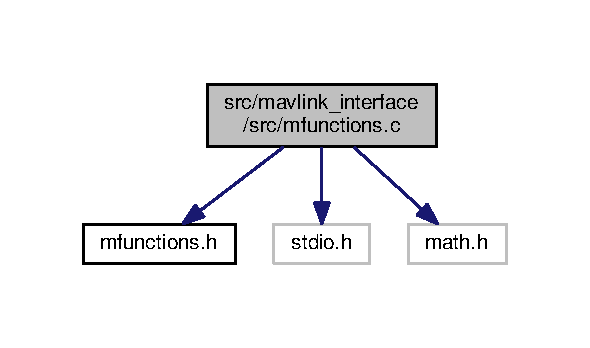
\includegraphics[width=283pt]{mfunctions_8c__incl}
\end{center}
\end{figure}
\subsection*{Functions}
\begin{DoxyCompactItemize}
\item 
float \hyperlink{mfunctions_8c_a4e7ac5bb03cc548079cceaa888e45a8a}{tan\+\_\+2pi} (int angle)
\item 
float \hyperlink{mfunctions_8c_a71ab9e1f160bb0627b405c3b043434e6}{Beta} (int angle)
\end{DoxyCompactItemize}
\subsection*{Variables}
\begin{DoxyCompactItemize}
\item 
float \hyperlink{mfunctions_8c_a7a108a522e73108b40c3b86c92f7b0c5}{tangent\+\_\+values\+\_\+buffer} \mbox{[}360\mbox{]}
\item 
float \hyperlink{mfunctions_8c_afe1ceabbe80d5b984deced9223258045}{Beta\+\_\+buffer} \mbox{[}360\mbox{]}
\end{DoxyCompactItemize}


\subsection{Function Documentation}
\index{mfunctions.\+c@{mfunctions.\+c}!Beta@{Beta}}
\index{Beta@{Beta}!mfunctions.\+c@{mfunctions.\+c}}
\subsubsection[{\texorpdfstring{Beta(int angle)}{Beta(int angle)}}]{\setlength{\rightskip}{0pt plus 5cm}float Beta (
\begin{DoxyParamCaption}
\item[{int}]{angle}
\end{DoxyParamCaption}
)}\hypertarget{mfunctions_8c_a71ab9e1f160bb0627b405c3b043434e6}{}\label{mfunctions_8c_a71ab9e1f160bb0627b405c3b043434e6}
\index{mfunctions.\+c@{mfunctions.\+c}!tan\+\_\+2pi@{tan\+\_\+2pi}}
\index{tan\+\_\+2pi@{tan\+\_\+2pi}!mfunctions.\+c@{mfunctions.\+c}}
\subsubsection[{\texorpdfstring{tan\+\_\+2pi(int angle)}{tan_2pi(int angle)}}]{\setlength{\rightskip}{0pt plus 5cm}float tan\+\_\+2pi (
\begin{DoxyParamCaption}
\item[{int}]{angle}
\end{DoxyParamCaption}
)}\hypertarget{mfunctions_8c_a4e7ac5bb03cc548079cceaa888e45a8a}{}\label{mfunctions_8c_a4e7ac5bb03cc548079cceaa888e45a8a}


\subsection{Variable Documentation}
\index{mfunctions.\+c@{mfunctions.\+c}!Beta\+\_\+buffer@{Beta\+\_\+buffer}}
\index{Beta\+\_\+buffer@{Beta\+\_\+buffer}!mfunctions.\+c@{mfunctions.\+c}}
\subsubsection[{\texorpdfstring{Beta\+\_\+buffer}{Beta_buffer}}]{\setlength{\rightskip}{0pt plus 5cm}float Beta\+\_\+buffer\mbox{[}360\mbox{]}}\hypertarget{mfunctions_8c_afe1ceabbe80d5b984deced9223258045}{}\label{mfunctions_8c_afe1ceabbe80d5b984deced9223258045}
{\bfseries Initial value\+:}
\begin{DoxyCode}
=\{1.000000,1.000152,1.000609,1.001373,1.002442,1.003820,1.005508,1.007510,1.009828,1.012465,1.015427,1.0187
      17,1.022340,1.026304,
                        1.030613,1.035276,1.040299,1.045692,1.051462,1.057621,1.064178,1.071145,1.078535,1.
      086360,1.094636,1.103378,1.112602,1.122326,
                        1.132570,1.143354,1.154700,1.166634,1.179178,1.192364,1.206218,1.220775,1.236068,1.
      252136,1.269019,1.286759,1.305408,1.325013,
                        1.345633,1.367327,1.390164,1.414214,1.439556,1.466279,1.494477,1.524253,1.555724,1.
      589016,1.624270,1.661640,1.701301,1.743447,
                        1.788292,1.836078,1.887080,1.941604,2.000000,2.062665,2.130054,2.202689,2.281172,2.
      366202,2.458594,2.559305,2.669466,2.790428,
                        2.923804,3.071554,3.236068,3.420304,3.627955,3.863703,4.133565,4.445412,4.809735,5.
      240845,5.758769,6.392453,7.185297,8.205511,
                        9.566776,11.473706,14.335579,19.107317,28.653709,57.298767,1.000000,57.298870,28.65
      3736,19.107328,14.335586,11.473709,9.566769,
                        8.205513,7.185298,6.392454,5.758770,5.240842,4.809733,4.445413,4.133565,3.863703,3.
      627955,3.420303,3.236068,3.071554,2.923805,
                        2.790428,2.669467,2.559304,2.458594,2.366201,2.281172,2.202689,2.130054,2.062665,2.
      000000,1.941604,1.887079,1.836078,1.788292,
                        1.743447,1.701301,1.661640,1.624270,1.589016,1.555724,1.524254,1.494476,1.466279,1.
      439556,1.414214,1.390164,1.367327,1.345633,
                        1.325013,1.305408,1.286759,1.269019,1.252136,1.236068,1.220775,1.206218,1.192364,1.
      179178,1.166634,1.154700,1.143354,1.132570,
                        1.122327,1.112602,1.103378,1.094636,1.086360,1.078535,1.071145,1.064178,1.057621,1.
      051462,1.045692,1.040299,1.035276,1.030613,
                        1.026304,1.022340,1.018717,1.015427,1.012465,1.009828,1.007510,1.005508,1.003820,1.
      002442,1.001373,1.000609,1.000152,1.000000,
                        1.000152,1.000609,1.001373,1.002442,1.003820,1.005508,1.007510,1.009828,1.012465,1.
      015427,1.018717,1.022340,1.026304,1.030613,
                        1.035276,1.040299,1.045692,1.051462,1.057621,1.064178,1.071145,1.078535,1.086360,1.
      094636,1.103378,1.112602,1.122326,1.132570,
                        1.143354,1.154700,1.166633,1.179178,1.192364,1.206218,1.220774,1.236068,1.252136,1.
      269018,1.286759,1.305408,1.325013,1.345633,
                        1.367327,1.390164,1.414214,1.439556,1.466279,1.494477,1.524253,1.555724,1.589016,1.
      624269,1.661640,1.701303,1.743447,1.788292,
                        1.836078,1.887079,1.941604,2.000000,2.062665,2.130054,2.202689,2.281173,2.366202,2.
      458594,2.559304,2.669466,2.790429,2.923805,
                        3.071554,3.236067,3.420301,3.627958,3.863705,4.133564,4.445409,4.809730,5.240847,5.
      758771,6.392451,7.185289,8.205523,9.566784,
                        11.473718,14.335572,19.107262,28.653881,57.299053,1.000000,57.298977,28.653862,19.1
      07252,14.335567,11.473714,9.566781,8.205523,
                        7.185288,6.392449,5.758771,5.240846,4.809739,4.445409,4.133564,3.863703,3.627957,3.
      420306,3.236067,3.071554,2.923805,2.790429,
                        2.669466,2.559304,2.458594,2.366202,2.281173,2.202689,2.130054,2.062665,2.000000,1.
      941604,1.887079,1.836078,1.788292,1.743447,
                        1.701303,1.661640,1.624269,1.589016,1.555724,1.524254,1.494476,1.466279,1.439556,1.
      414214,1.390163,1.367327,1.345633,1.325013,
                        1.305408,1.286759,1.269018,1.252136,1.236068,1.220775,1.206218,1.192363,1.179178,1.
      166634,1.154701,1.143354,1.132570,1.122326,
                        1.112602,1.103378,1.094636,1.086360,1.078535,1.071145,1.064178,1.057620,1.051462,1.
      045692,1.040299,1.035276,1.030613,1.026304,
                        1.022340,1.018717,1.015427,1.012465,1.009828,1.007510,1.005508,1.003820,1.002442,1.
      001373,1.000609,1.000152\}
\end{DoxyCode}
\index{mfunctions.\+c@{mfunctions.\+c}!tangent\+\_\+values\+\_\+buffer@{tangent\+\_\+values\+\_\+buffer}}
\index{tangent\+\_\+values\+\_\+buffer@{tangent\+\_\+values\+\_\+buffer}!mfunctions.\+c@{mfunctions.\+c}}
\subsubsection[{\texorpdfstring{tangent\+\_\+values\+\_\+buffer}{tangent_values_buffer}}]{\setlength{\rightskip}{0pt plus 5cm}float tangent\+\_\+values\+\_\+buffer\mbox{[}360\mbox{]}}\hypertarget{mfunctions_8c_a7a108a522e73108b40c3b86c92f7b0c5}{}\label{mfunctions_8c_a7a108a522e73108b40c3b86c92f7b0c5}
{\bfseries Initial value\+:}
\begin{DoxyCode}
=\{0.000000,0.017455,0.034921,0.052408,0.069927,0.087489,0.105104,0.122785,0.140541,0.158384,0.176327,0.1943
      80,0.212557,
                                0.230868,0.249328,0.267949,0.286745,0.305731,0.324920,0.344328,0.363970,0.3
      83864,0.404026,0.424475,0.445229,0.466308,
                                0.487733,0.509525,0.531709,0.554309,0.577350,0.600861,0.624869,0.649408,0.6
      74508,0.700208,0.726543,0.753554,0.781286,
                                0.809784,0.839100,0.869287,0.900404,0.932515,0.965689,1.000000,1.035530,1.0
      72369,1.110613,1.150368,1.191754,1.234897,
                                1.279942,1.327045,1.376382,1.428148,1.482561,1.539865,1.600335,1.664280,1.7
      32051,1.804048,1.880726,1.962610,2.050304,
                                2.144507,2.246037,2.355853,2.475086,2.605089,2.747477,2.904211,3.077684,3.2
      70853,3.487414,3.732050,4.010781,4.331476,
                                4.704631,5.144556,5.671280,6.313751,7.115370,8.144348,9.514368,11.430045,14
      .300658,19.081131,28.636255,57.290039,
                                0.000000,-57.290142,-28.636282,-19.081142,-14.300665,-11.430049,-9.514360,-
      8.144350,-7.115371,-6.313752,-5.671281,
                                -5.144553,-4.704629,-4.331477,-4.010781,-3.732051,-3.487414,-3.270852,-3.07
      7683,-2.904211,-2.747478,-2.605089,-2.475087,
                                -2.355852,-2.246037,-2.144506,-2.050304,-1.962610,-1.880726,-1.804048,-1.73
      2051,-1.664280,-1.600334,-1.539865,-1.482561,
                                -1.428148,-1.376382,-1.327045,-1.279942,-1.234897,-1.191754,-1.150369,-1.11
      0612,-1.072369,-1.035530,-1.000000,-0.965689,
                                -0.932515,-0.900404,-0.869287,-0.839100,-0.809784,-0.781286,-0.753554,-0.72
      6542,-0.700208,-0.674508,-0.649408,-0.624869,
                                -0.600861,-0.577350,-0.554309,-0.531709,-0.509526,-0.487733,-0.466308,-0.44
      5229,-0.424475,-0.404026,-0.383864,-0.363970,
                                -0.344328,-0.324920,-0.305731,-0.286745,-0.267949,-0.249328,-0.230868,-0.21
      2556,-0.194380,-0.176327,-0.158384,-0.140541,
                                -0.122784,-0.105104,-0.087489,-0.069927,-0.052408,-0.034921,-0.017455,0.000
      000,0.017455,0.034921,0.052408,0.069927,0.087489,
                                0.105104,0.122785,0.140541,0.158384,0.176327,0.194380,0.212557,0.230868,0.2
      49328,0.267949,0.286745,0.305731,0.324920,0.344328,
                                0.363970,0.383864,0.404026,0.424475,0.445229,0.466308,0.487732,0.509525,0.5
      31709,0.554309,0.577350,0.600860,0.624869,0.649408,
                                0.674509,0.700207,0.726543,0.753554,0.781285,0.809784,0.839100,0.869287,0.9
      00404,0.932515,0.965689,1.000000,1.035530,1.072369,
                                1.110613,1.150368,1.191754,1.234897,1.279941,1.327044,1.376383,1.428148,1.4
      82561,1.539865,1.600334,1.664280,1.732051,1.804048,
                                1.880726,1.962610,2.050305,2.144507,2.246037,2.355852,2.475085,2.605090,2.7
      47478,2.904211,3.077682,3.270850,3.487417,3.732052,
                                4.010780,4.331473,4.704625,5.144558,5.671283,6.313749,7.115362,8.144361,9.5
      14377,11.430057,14.300652,19.081076,28.636425,
                                57.290325, 0.000000,-57.290249,-28.636406,-19.081066,-14.300647,-11.430053,
      -9.514374,-8.144361,-7.115361,-6.313748,
                                -5.671283,-5.144557,-4.704635,-4.331473,-4.010780,-3.732051,-3.487416,-3.27
      0855,-3.077682,-2.904211,-2.747478,-2.605090,
                                -2.475085,-2.355852,-2.246037,-2.144507,-2.050305,-1.962610,-1.880726,-1.80
      4048,-1.732051,-1.664280,-1.600334,-1.539865,
                                -1.482561,-1.428148,-1.376383,-1.327044,-1.279941,-1.234897,-1.191754,-1.15
      0369,-1.110612,-1.072369,-1.035530,-1.000000,
                                -0.965688,-0.932515,-0.900404,-0.869287,-0.839100,-0.809784,-0.781285,-0.75
      3554,-0.726543,-0.700208,-0.674508,-0.649407,
                                -0.624869,-0.600861,-0.577351,-0.554309,-0.531709,-0.509525,-0.487733,-0.46
      6308,-0.445228,-0.424475,-0.404026,-0.383864,
                                -0.363970,-0.344327,-0.324920,-0.305731,-0.286746,-0.267949,-0.249328,-0.23
      0868,-0.212557,-0.194380,-0.176327,-0.158384,
                                -0.140541,-0.122785,-0.105104,-0.087488,-0.069927,-0.052408,-0.034921,-0.01
      7455,\}
\end{DoxyCode}

\hypertarget{mfunctions_8d}{}\section{src/mavlink\+\_\+interface/src/mfunctions.d File Reference}
\label{mfunctions_8d}\index{src/mavlink\+\_\+interface/src/mfunctions.\+d@{src/mavlink\+\_\+interface/src/mfunctions.\+d}}

\hypertarget{cad__utils_8c}{}\section{src/piface\+C\+A\+D/cad\+\_\+utils.c File Reference}
\label{cad__utils_8c}\index{src/piface\+C\+A\+D/cad\+\_\+utils.\+c@{src/piface\+C\+A\+D/cad\+\_\+utils.\+c}}
{\ttfamily \#include \char`\"{}cad\+\_\+utils.\+h\char`\"{}}\\*
Include dependency graph for cad\+\_\+utils.\+c\+:\nopagebreak
\begin{figure}[H]
\begin{center}
\leavevmode
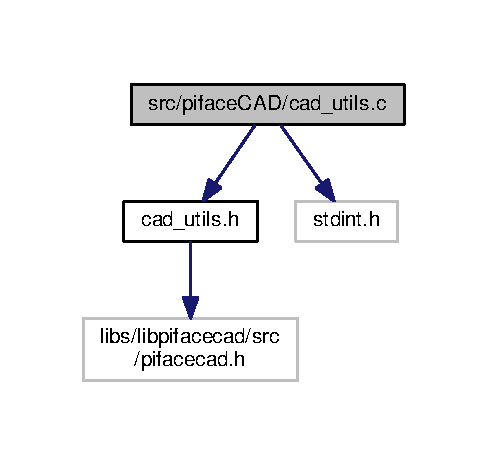
\includegraphics[width=234pt]{cad__utils_8c__incl}
\end{center}
\end{figure}
\subsection*{Functions}
\begin{DoxyCompactItemize}
\item 
int \hyperlink{cad__utils_8c_a273648c3e0d370c3a934fa1179b58bd6}{init\+\_\+cad} ()
\item 
int \hyperlink{cad__utils_8c_a75deb7a77966fea4233926bd14d41a69}{print\+\_\+to\+\_\+cad} (char $\ast$str)
\item 
void \hyperlink{cad__utils_8c_ac9032dc379c2e478bedcd77cbf100cfc}{close\+\_\+cad} ()
\item 
void \hyperlink{cad__utils_8c_a25588fbe02610e238ab76c852fe2eefc}{clear\+\_\+cad} ()
\end{DoxyCompactItemize}


\subsection{Function Documentation}
\index{cad\+\_\+utils.\+c@{cad\+\_\+utils.\+c}!clear\+\_\+cad@{clear\+\_\+cad}}
\index{clear\+\_\+cad@{clear\+\_\+cad}!cad\+\_\+utils.\+c@{cad\+\_\+utils.\+c}}
\subsubsection[{\texorpdfstring{clear\+\_\+cad()}{clear_cad()}}]{\setlength{\rightskip}{0pt plus 5cm}void clear\+\_\+cad (
\begin{DoxyParamCaption}
{}
\end{DoxyParamCaption}
)}\hypertarget{cad__utils_8c_a25588fbe02610e238ab76c852fe2eefc}{}\label{cad__utils_8c_a25588fbe02610e238ab76c852fe2eefc}
\index{cad\+\_\+utils.\+c@{cad\+\_\+utils.\+c}!close\+\_\+cad@{close\+\_\+cad}}
\index{close\+\_\+cad@{close\+\_\+cad}!cad\+\_\+utils.\+c@{cad\+\_\+utils.\+c}}
\subsubsection[{\texorpdfstring{close\+\_\+cad()}{close_cad()}}]{\setlength{\rightskip}{0pt plus 5cm}void close\+\_\+cad (
\begin{DoxyParamCaption}
{}
\end{DoxyParamCaption}
)}\hypertarget{cad__utils_8c_ac9032dc379c2e478bedcd77cbf100cfc}{}\label{cad__utils_8c_ac9032dc379c2e478bedcd77cbf100cfc}
\index{cad\+\_\+utils.\+c@{cad\+\_\+utils.\+c}!init\+\_\+cad@{init\+\_\+cad}}
\index{init\+\_\+cad@{init\+\_\+cad}!cad\+\_\+utils.\+c@{cad\+\_\+utils.\+c}}
\subsubsection[{\texorpdfstring{init\+\_\+cad()}{init_cad()}}]{\setlength{\rightskip}{0pt plus 5cm}int init\+\_\+cad (
\begin{DoxyParamCaption}
{}
\end{DoxyParamCaption}
)}\hypertarget{cad__utils_8c_a273648c3e0d370c3a934fa1179b58bd6}{}\label{cad__utils_8c_a273648c3e0d370c3a934fa1179b58bd6}
\index{cad\+\_\+utils.\+c@{cad\+\_\+utils.\+c}!print\+\_\+to\+\_\+cad@{print\+\_\+to\+\_\+cad}}
\index{print\+\_\+to\+\_\+cad@{print\+\_\+to\+\_\+cad}!cad\+\_\+utils.\+c@{cad\+\_\+utils.\+c}}
\subsubsection[{\texorpdfstring{print\+\_\+to\+\_\+cad(char $\ast$str)}{print_to_cad(char *str)}}]{\setlength{\rightskip}{0pt plus 5cm}int print\+\_\+to\+\_\+cad (
\begin{DoxyParamCaption}
\item[{char $\ast$}]{str}
\end{DoxyParamCaption}
)}\hypertarget{cad__utils_8c_a75deb7a77966fea4233926bd14d41a69}{}\label{cad__utils_8c_a75deb7a77966fea4233926bd14d41a69}

\hypertarget{cad__utils_8d}{}\section{src/piface\+C\+A\+D/cad\+\_\+utils.d File Reference}
\label{cad__utils_8d}\index{src/piface\+C\+A\+D/cad\+\_\+utils.\+d@{src/piface\+C\+A\+D/cad\+\_\+utils.\+d}}

\hypertarget{cad__utils_8h}{}\section{src/piface\+C\+A\+D/cad\+\_\+utils.h File Reference}
\label{cad__utils_8h}\index{src/piface\+C\+A\+D/cad\+\_\+utils.\+h@{src/piface\+C\+A\+D/cad\+\_\+utils.\+h}}
{\ttfamily \#include $<$libs/libpifacecad/src/pifacecad.\+h$>$}\\*
Include dependency graph for cad\+\_\+utils.\+h\+:
\nopagebreak
\begin{figure}[H]
\begin{center}
\leavevmode
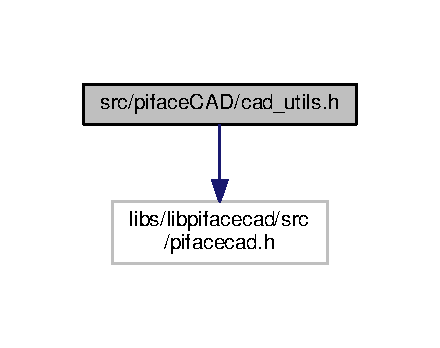
\includegraphics[width=211pt]{cad__utils_8h__incl}
\end{center}
\end{figure}
This graph shows which files directly or indirectly include this file\+:
\nopagebreak
\begin{figure}[H]
\begin{center}
\leavevmode
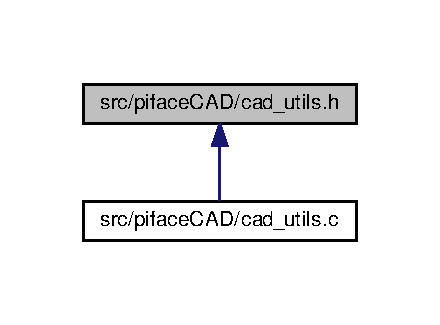
\includegraphics[width=211pt]{cad__utils_8h__dep__incl}
\end{center}
\end{figure}
\subsection*{Functions}
\begin{DoxyCompactItemize}
\item 
int \hyperlink{cad__utils_8h_a273648c3e0d370c3a934fa1179b58bd6}{init\+\_\+cad} ()
\item 
int \hyperlink{cad__utils_8h_a75deb7a77966fea4233926bd14d41a69}{print\+\_\+to\+\_\+cad} (char $\ast$str)
\item 
void \hyperlink{cad__utils_8h_ac9032dc379c2e478bedcd77cbf100cfc}{close\+\_\+cad} ()
\item 
void \hyperlink{cad__utils_8h_a25588fbe02610e238ab76c852fe2eefc}{clear\+\_\+cad} ()
\end{DoxyCompactItemize}


\subsection{Function Documentation}
\index{cad\+\_\+utils.\+h@{cad\+\_\+utils.\+h}!clear\+\_\+cad@{clear\+\_\+cad}}
\index{clear\+\_\+cad@{clear\+\_\+cad}!cad\+\_\+utils.\+h@{cad\+\_\+utils.\+h}}
\subsubsection[{\texorpdfstring{clear\+\_\+cad()}{clear_cad()}}]{\setlength{\rightskip}{0pt plus 5cm}void clear\+\_\+cad (
\begin{DoxyParamCaption}
{}
\end{DoxyParamCaption}
)}\hypertarget{cad__utils_8h_a25588fbe02610e238ab76c852fe2eefc}{}\label{cad__utils_8h_a25588fbe02610e238ab76c852fe2eefc}
\index{cad\+\_\+utils.\+h@{cad\+\_\+utils.\+h}!close\+\_\+cad@{close\+\_\+cad}}
\index{close\+\_\+cad@{close\+\_\+cad}!cad\+\_\+utils.\+h@{cad\+\_\+utils.\+h}}
\subsubsection[{\texorpdfstring{close\+\_\+cad()}{close_cad()}}]{\setlength{\rightskip}{0pt plus 5cm}void close\+\_\+cad (
\begin{DoxyParamCaption}
{}
\end{DoxyParamCaption}
)}\hypertarget{cad__utils_8h_ac9032dc379c2e478bedcd77cbf100cfc}{}\label{cad__utils_8h_ac9032dc379c2e478bedcd77cbf100cfc}
\index{cad\+\_\+utils.\+h@{cad\+\_\+utils.\+h}!init\+\_\+cad@{init\+\_\+cad}}
\index{init\+\_\+cad@{init\+\_\+cad}!cad\+\_\+utils.\+h@{cad\+\_\+utils.\+h}}
\subsubsection[{\texorpdfstring{init\+\_\+cad()}{init_cad()}}]{\setlength{\rightskip}{0pt plus 5cm}int init\+\_\+cad (
\begin{DoxyParamCaption}
{}
\end{DoxyParamCaption}
)}\hypertarget{cad__utils_8h_a273648c3e0d370c3a934fa1179b58bd6}{}\label{cad__utils_8h_a273648c3e0d370c3a934fa1179b58bd6}
\index{cad\+\_\+utils.\+h@{cad\+\_\+utils.\+h}!print\+\_\+to\+\_\+cad@{print\+\_\+to\+\_\+cad}}
\index{print\+\_\+to\+\_\+cad@{print\+\_\+to\+\_\+cad}!cad\+\_\+utils.\+h@{cad\+\_\+utils.\+h}}
\subsubsection[{\texorpdfstring{print\+\_\+to\+\_\+cad(char $\ast$str)}{print_to_cad(char *str)}}]{\setlength{\rightskip}{0pt plus 5cm}int print\+\_\+to\+\_\+cad (
\begin{DoxyParamCaption}
\item[{char $\ast$}]{str}
\end{DoxyParamCaption}
)}\hypertarget{cad__utils_8h_a75deb7a77966fea4233926bd14d41a69}{}\label{cad__utils_8h_a75deb7a77966fea4233926bd14d41a69}

\hypertarget{parser_8c}{}\section{src/\+R\+Pi\+G\+P\+S\+Demo/parser.c File Reference}
\label{parser_8c}\index{src/\+R\+Pi\+G\+P\+S\+Demo/parser.\+c@{src/\+R\+Pi\+G\+P\+S\+Demo/parser.\+c}}
{\ttfamily \#include \char`\"{}parser.\+h\char`\"{}}\\*
{\ttfamily \#include $<$string.\+h$>$}\\*
{\ttfamily \#include $<$stdlib.\+h$>$}\\*
{\ttfamily \#include $<$stdio.\+h$>$}\\*
Include dependency graph for parser.\+c\+:
\nopagebreak
\begin{figure}[H]
\begin{center}
\leavevmode
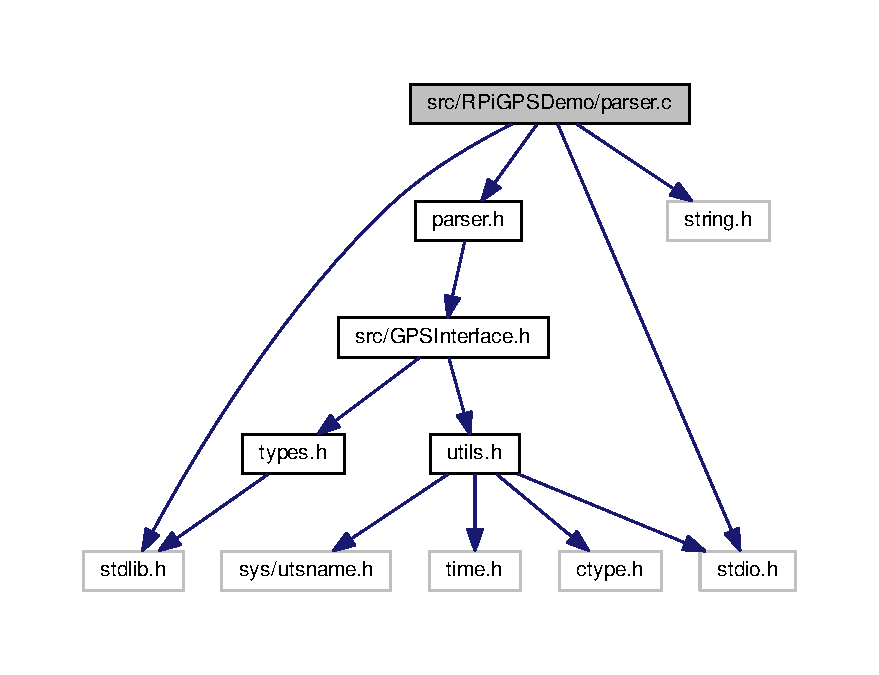
\includegraphics[width=350pt]{parser_8c__incl}
\end{center}
\end{figure}
\subsection*{Functions}
\begin{DoxyCompactItemize}
\item 
int \hyperlink{parser_8c_ac5b07dced6a5c7d5da22e87e9786d7e1}{parse\+\_\+nmea} (char $\ast$sentence, \hyperlink{struct_full_g_p_s_data}{Full\+G\+P\+S\+Data} $\ast$samp)
\item 
int \hyperlink{parser_8c_a5c6b8157da5d565140f4191c7c1fb0cd}{validate\+\_\+checksum} (char $\ast$nmea)
\item 
void \hyperlink{parser_8c_a4cb4cd3df7023bf69341b657ae8d7bdc}{parse\+\_\+gsa} (\hyperlink{structgsa}{gsa} $\ast$\hyperlink{structgsa}{gsa}, char $\ast$nmea)
\item 
void \hyperlink{parser_8c_a759c53be0d7fd59939ea06003c2c080f}{parse\+\_\+gll} (\hyperlink{structgll}{gll} $\ast$samp, char $\ast$nmea)
\item 
void \hyperlink{parser_8c_a1aab6de4fcd029e49dbf845194b6fa55}{parse\+\_\+vtg} (\hyperlink{structvtg}{vtg} $\ast$samp, char $\ast$nmea)
\item 
void \hyperlink{parser_8c_a0e3b05cfdd44f7bcc48b5d227a4184fd}{parse\+\_\+gga\+\_\+new} (\hyperlink{structgga}{gga} $\ast$samp, char $\ast$nmea)
\item 
void \hyperlink{parser_8c_a15635b5b7940be5bef8123cd3d8d1a8d}{parse\+\_\+rmc\+\_\+new} (\hyperlink{structrmc}{rmc} $\ast$samp, char $\ast$nmea)
\item 
void \hyperlink{parser_8c_a3e763ea09575f4a874d10ccab857cd05}{parse\+\_\+gga} (\hyperlink{structgga}{gga} $\ast$samp, char $\ast$nmea)
\item 
void \hyperlink{parser_8c_a400c090e598ddcbd64aa6946a1a2ce71}{parse\+\_\+rmc} (\hyperlink{structrmc}{rmc} $\ast$samp, char $\ast$nmea)
\item 
\hyperlink{types_8h_af6a258d8f3ee5206d682d799316314b1}{bool} \hyperlink{parser_8c_a09fade3eab39798f55135e16c99e913a}{is\+\_\+nmea\+\_\+txt} (char $\ast$nmea)
\end{DoxyCompactItemize}


\subsection{Function Documentation}
\index{parser.\+c@{parser.\+c}!is\+\_\+nmea\+\_\+txt@{is\+\_\+nmea\+\_\+txt}}
\index{is\+\_\+nmea\+\_\+txt@{is\+\_\+nmea\+\_\+txt}!parser.\+c@{parser.\+c}}
\subsubsection[{\texorpdfstring{is\+\_\+nmea\+\_\+txt(char $\ast$nmea)}{is_nmea_txt(char *nmea)}}]{\setlength{\rightskip}{0pt plus 5cm}{\bf bool} is\+\_\+nmea\+\_\+txt (
\begin{DoxyParamCaption}
\item[{char $\ast$}]{nmea}
\end{DoxyParamCaption}
)}\hypertarget{parser_8c_a09fade3eab39798f55135e16c99e913a}{}\label{parser_8c_a09fade3eab39798f55135e16c99e913a}
\index{parser.\+c@{parser.\+c}!parse\+\_\+gga@{parse\+\_\+gga}}
\index{parse\+\_\+gga@{parse\+\_\+gga}!parser.\+c@{parser.\+c}}
\subsubsection[{\texorpdfstring{parse\+\_\+gga(gga $\ast$samp, char $\ast$nmea)}{parse_gga(gga *samp, char *nmea)}}]{\setlength{\rightskip}{0pt plus 5cm}void parse\+\_\+gga (
\begin{DoxyParamCaption}
\item[{{\bf gga} $\ast$}]{samp, }
\item[{char $\ast$}]{nmea}
\end{DoxyParamCaption}
)}\hypertarget{parser_8c_a3e763ea09575f4a874d10ccab857cd05}{}\label{parser_8c_a3e763ea09575f4a874d10ccab857cd05}
\index{parser.\+c@{parser.\+c}!parse\+\_\+gga\+\_\+new@{parse\+\_\+gga\+\_\+new}}
\index{parse\+\_\+gga\+\_\+new@{parse\+\_\+gga\+\_\+new}!parser.\+c@{parser.\+c}}
\subsubsection[{\texorpdfstring{parse\+\_\+gga\+\_\+new(gga $\ast$samp, char $\ast$nmea)}{parse_gga_new(gga *samp, char *nmea)}}]{\setlength{\rightskip}{0pt plus 5cm}void parse\+\_\+gga\+\_\+new (
\begin{DoxyParamCaption}
\item[{{\bf gga} $\ast$}]{samp, }
\item[{char $\ast$}]{nmea}
\end{DoxyParamCaption}
)}\hypertarget{parser_8c_a0e3b05cfdd44f7bcc48b5d227a4184fd}{}\label{parser_8c_a0e3b05cfdd44f7bcc48b5d227a4184fd}
\index{parser.\+c@{parser.\+c}!parse\+\_\+gll@{parse\+\_\+gll}}
\index{parse\+\_\+gll@{parse\+\_\+gll}!parser.\+c@{parser.\+c}}
\subsubsection[{\texorpdfstring{parse\+\_\+gll(gll $\ast$samp, char $\ast$nmea)}{parse_gll(gll *samp, char *nmea)}}]{\setlength{\rightskip}{0pt plus 5cm}void parse\+\_\+gll (
\begin{DoxyParamCaption}
\item[{{\bf gll} $\ast$}]{samp, }
\item[{char $\ast$}]{nmea}
\end{DoxyParamCaption}
)}\hypertarget{parser_8c_a759c53be0d7fd59939ea06003c2c080f}{}\label{parser_8c_a759c53be0d7fd59939ea06003c2c080f}
\index{parser.\+c@{parser.\+c}!parse\+\_\+gsa@{parse\+\_\+gsa}}
\index{parse\+\_\+gsa@{parse\+\_\+gsa}!parser.\+c@{parser.\+c}}
\subsubsection[{\texorpdfstring{parse\+\_\+gsa(gsa $\ast$gsa, char $\ast$nmea)}{parse_gsa(gsa *gsa, char *nmea)}}]{\setlength{\rightskip}{0pt plus 5cm}void parse\+\_\+gsa (
\begin{DoxyParamCaption}
\item[{{\bf gsa} $\ast$}]{gsa, }
\item[{char $\ast$}]{nmea}
\end{DoxyParamCaption}
)}\hypertarget{parser_8c_a4cb4cd3df7023bf69341b657ae8d7bdc}{}\label{parser_8c_a4cb4cd3df7023bf69341b657ae8d7bdc}
\index{parser.\+c@{parser.\+c}!parse\+\_\+nmea@{parse\+\_\+nmea}}
\index{parse\+\_\+nmea@{parse\+\_\+nmea}!parser.\+c@{parser.\+c}}
\subsubsection[{\texorpdfstring{parse\+\_\+nmea(char $\ast$sentence, Full\+G\+P\+S\+Data $\ast$samp)}{parse_nmea(char *sentence, FullGPSData *samp)}}]{\setlength{\rightskip}{0pt plus 5cm}int parse\+\_\+nmea (
\begin{DoxyParamCaption}
\item[{char $\ast$}]{sentence, }
\item[{{\bf Full\+G\+P\+S\+Data} $\ast$}]{samp}
\end{DoxyParamCaption}
)}\hypertarget{parser_8c_ac5b07dced6a5c7d5da22e87e9786d7e1}{}\label{parser_8c_ac5b07dced6a5c7d5da22e87e9786d7e1}
\index{parser.\+c@{parser.\+c}!parse\+\_\+rmc@{parse\+\_\+rmc}}
\index{parse\+\_\+rmc@{parse\+\_\+rmc}!parser.\+c@{parser.\+c}}
\subsubsection[{\texorpdfstring{parse\+\_\+rmc(rmc $\ast$samp, char $\ast$nmea)}{parse_rmc(rmc *samp, char *nmea)}}]{\setlength{\rightskip}{0pt plus 5cm}void parse\+\_\+rmc (
\begin{DoxyParamCaption}
\item[{{\bf rmc} $\ast$}]{samp, }
\item[{char $\ast$}]{nmea}
\end{DoxyParamCaption}
)}\hypertarget{parser_8c_a400c090e598ddcbd64aa6946a1a2ce71}{}\label{parser_8c_a400c090e598ddcbd64aa6946a1a2ce71}
\index{parser.\+c@{parser.\+c}!parse\+\_\+rmc\+\_\+new@{parse\+\_\+rmc\+\_\+new}}
\index{parse\+\_\+rmc\+\_\+new@{parse\+\_\+rmc\+\_\+new}!parser.\+c@{parser.\+c}}
\subsubsection[{\texorpdfstring{parse\+\_\+rmc\+\_\+new(rmc $\ast$samp, char $\ast$nmea)}{parse_rmc_new(rmc *samp, char *nmea)}}]{\setlength{\rightskip}{0pt plus 5cm}void parse\+\_\+rmc\+\_\+new (
\begin{DoxyParamCaption}
\item[{{\bf rmc} $\ast$}]{samp, }
\item[{char $\ast$}]{nmea}
\end{DoxyParamCaption}
)}\hypertarget{parser_8c_a15635b5b7940be5bef8123cd3d8d1a8d}{}\label{parser_8c_a15635b5b7940be5bef8123cd3d8d1a8d}
\index{parser.\+c@{parser.\+c}!parse\+\_\+vtg@{parse\+\_\+vtg}}
\index{parse\+\_\+vtg@{parse\+\_\+vtg}!parser.\+c@{parser.\+c}}
\subsubsection[{\texorpdfstring{parse\+\_\+vtg(vtg $\ast$samp, char $\ast$nmea)}{parse_vtg(vtg *samp, char *nmea)}}]{\setlength{\rightskip}{0pt plus 5cm}void parse\+\_\+vtg (
\begin{DoxyParamCaption}
\item[{{\bf vtg} $\ast$}]{samp, }
\item[{char $\ast$}]{nmea}
\end{DoxyParamCaption}
)}\hypertarget{parser_8c_a1aab6de4fcd029e49dbf845194b6fa55}{}\label{parser_8c_a1aab6de4fcd029e49dbf845194b6fa55}
\index{parser.\+c@{parser.\+c}!validate\+\_\+checksum@{validate\+\_\+checksum}}
\index{validate\+\_\+checksum@{validate\+\_\+checksum}!parser.\+c@{parser.\+c}}
\subsubsection[{\texorpdfstring{validate\+\_\+checksum(char $\ast$nmea)}{validate_checksum(char *nmea)}}]{\setlength{\rightskip}{0pt plus 5cm}int validate\+\_\+checksum (
\begin{DoxyParamCaption}
\item[{char $\ast$}]{nmea}
\end{DoxyParamCaption}
)}\hypertarget{parser_8c_a5c6b8157da5d565140f4191c7c1fb0cd}{}\label{parser_8c_a5c6b8157da5d565140f4191c7c1fb0cd}

\hypertarget{parser_8d}{}\section{src/\+R\+Pi\+G\+P\+S\+Demo/parser.d File Reference}
\label{parser_8d}\index{src/\+R\+Pi\+G\+P\+S\+Demo/parser.\+d@{src/\+R\+Pi\+G\+P\+S\+Demo/parser.\+d}}

\hypertarget{parser_8h}{}\section{src/\+R\+Pi\+G\+P\+S\+Demo/parser.h File Reference}
\label{parser_8h}\index{src/\+R\+Pi\+G\+P\+S\+Demo/parser.\+h@{src/\+R\+Pi\+G\+P\+S\+Demo/parser.\+h}}
{\ttfamily \#include $<$src/\+G\+P\+S\+Interface.\+h$>$}\\*
Include dependency graph for parser.\+h\+:
\nopagebreak
\begin{figure}[H]
\begin{center}
\leavevmode
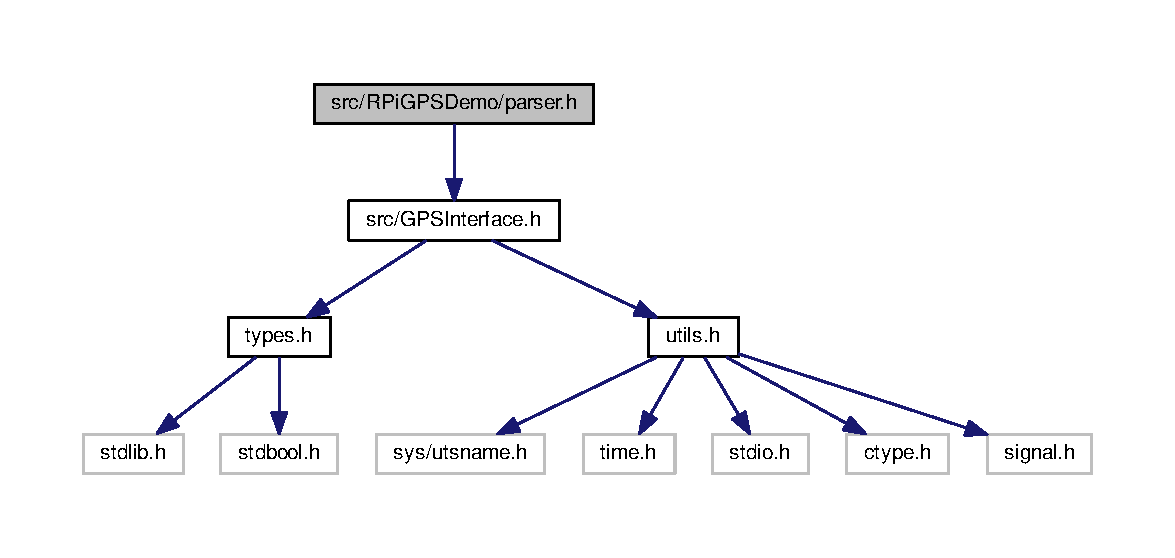
\includegraphics[width=350pt]{parser_8h__incl}
\end{center}
\end{figure}
This graph shows which files directly or indirectly include this file\+:\nopagebreak
\begin{figure}[H]
\begin{center}
\leavevmode
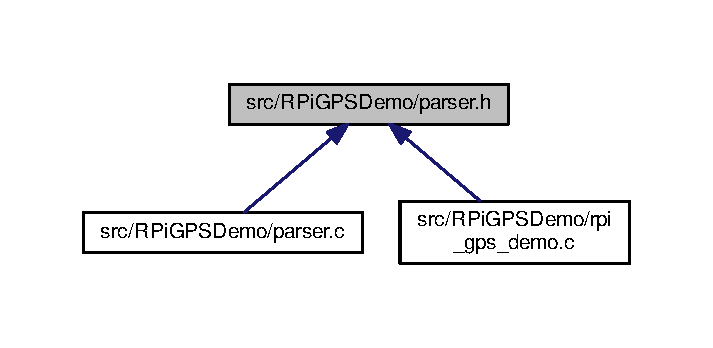
\includegraphics[width=342pt]{parser_8h__dep__incl}
\end{center}
\end{figure}
\subsection*{Macros}
\begin{DoxyCompactItemize}
\item 
\#define \hyperlink{parser_8h_af905d990565fd8441c0429728f803d4d}{C\+H\+E\+C\+K\+S\+U\+M\+\_\+\+OK}~0
\item 
\#define \hyperlink{parser_8h_a801103d15d79b01646bcee50855d4f3b}{C\+H\+E\+C\+K\+S\+U\+M\+\_\+\+E\+RR}~1
\end{DoxyCompactItemize}
\subsection*{Functions}
\begin{DoxyCompactItemize}
\item 
int \hyperlink{parser_8h_ac5b07dced6a5c7d5da22e87e9786d7e1}{parse\+\_\+nmea} (char $\ast$sentence, \hyperlink{struct_full_g_p_s_data}{Full\+G\+P\+S\+Data} $\ast$samp)
\item 
int \hyperlink{parser_8h_a5c6b8157da5d565140f4191c7c1fb0cd}{validate\+\_\+checksum} (char $\ast$nmea)
\item 
bool \hyperlink{parser_8h_a09fade3eab39798f55135e16c99e913a}{is\+\_\+nmea\+\_\+txt} (char $\ast$nmea)
\item 
void \hyperlink{parser_8h_a3e763ea09575f4a874d10ccab857cd05}{parse\+\_\+gga} (\hyperlink{structgga}{gga} $\ast$samp, char $\ast$nmea)
\item 
void \hyperlink{parser_8h_a400c090e598ddcbd64aa6946a1a2ce71}{parse\+\_\+rmc} (\hyperlink{structrmc}{rmc} $\ast$samp, char $\ast$nmea)
\item 
void \hyperlink{parser_8h_a15635b5b7940be5bef8123cd3d8d1a8d}{parse\+\_\+rmc\+\_\+new} (\hyperlink{structrmc}{rmc} $\ast$samp, char $\ast$nmea)
\item 
void \hyperlink{parser_8h_a0e3b05cfdd44f7bcc48b5d227a4184fd}{parse\+\_\+gga\+\_\+new} (\hyperlink{structgga}{gga} $\ast$samp, char $\ast$nmea)
\item 
void \hyperlink{parser_8h_ae15d9d4220caa6b7059580767d5406bd}{parse\+\_\+gsa} (\hyperlink{structgsa}{gsa} $\ast$samp, char $\ast$nmea)
\item 
void \hyperlink{parser_8h_a759c53be0d7fd59939ea06003c2c080f}{parse\+\_\+gll} (\hyperlink{structgll}{gll} $\ast$samp, char $\ast$nmea)
\item 
void \hyperlink{parser_8h_a1aab6de4fcd029e49dbf845194b6fa55}{parse\+\_\+vtg} (\hyperlink{structvtg}{vtg} $\ast$samp, char $\ast$nmea)
\end{DoxyCompactItemize}


\subsection{Macro Definition Documentation}
\index{parser.\+h@{parser.\+h}!C\+H\+E\+C\+K\+S\+U\+M\+\_\+\+E\+RR@{C\+H\+E\+C\+K\+S\+U\+M\+\_\+\+E\+RR}}
\index{C\+H\+E\+C\+K\+S\+U\+M\+\_\+\+E\+RR@{C\+H\+E\+C\+K\+S\+U\+M\+\_\+\+E\+RR}!parser.\+h@{parser.\+h}}
\subsubsection[{\texorpdfstring{C\+H\+E\+C\+K\+S\+U\+M\+\_\+\+E\+RR}{CHECKSUM_ERR}}]{\setlength{\rightskip}{0pt plus 5cm}\#define C\+H\+E\+C\+K\+S\+U\+M\+\_\+\+E\+RR~1}\hypertarget{parser_8h_a801103d15d79b01646bcee50855d4f3b}{}\label{parser_8h_a801103d15d79b01646bcee50855d4f3b}
\index{parser.\+h@{parser.\+h}!C\+H\+E\+C\+K\+S\+U\+M\+\_\+\+OK@{C\+H\+E\+C\+K\+S\+U\+M\+\_\+\+OK}}
\index{C\+H\+E\+C\+K\+S\+U\+M\+\_\+\+OK@{C\+H\+E\+C\+K\+S\+U\+M\+\_\+\+OK}!parser.\+h@{parser.\+h}}
\subsubsection[{\texorpdfstring{C\+H\+E\+C\+K\+S\+U\+M\+\_\+\+OK}{CHECKSUM_OK}}]{\setlength{\rightskip}{0pt plus 5cm}\#define C\+H\+E\+C\+K\+S\+U\+M\+\_\+\+OK~0}\hypertarget{parser_8h_af905d990565fd8441c0429728f803d4d}{}\label{parser_8h_af905d990565fd8441c0429728f803d4d}


\subsection{Function Documentation}
\index{parser.\+h@{parser.\+h}!is\+\_\+nmea\+\_\+txt@{is\+\_\+nmea\+\_\+txt}}
\index{is\+\_\+nmea\+\_\+txt@{is\+\_\+nmea\+\_\+txt}!parser.\+h@{parser.\+h}}
\subsubsection[{\texorpdfstring{is\+\_\+nmea\+\_\+txt(char $\ast$nmea)}{is_nmea_txt(char *nmea)}}]{\setlength{\rightskip}{0pt plus 5cm}bool is\+\_\+nmea\+\_\+txt (
\begin{DoxyParamCaption}
\item[{char $\ast$}]{nmea}
\end{DoxyParamCaption}
)}\hypertarget{parser_8h_a09fade3eab39798f55135e16c99e913a}{}\label{parser_8h_a09fade3eab39798f55135e16c99e913a}
\index{parser.\+h@{parser.\+h}!parse\+\_\+gga@{parse\+\_\+gga}}
\index{parse\+\_\+gga@{parse\+\_\+gga}!parser.\+h@{parser.\+h}}
\subsubsection[{\texorpdfstring{parse\+\_\+gga(gga $\ast$samp, char $\ast$nmea)}{parse_gga(gga *samp, char *nmea)}}]{\setlength{\rightskip}{0pt plus 5cm}void parse\+\_\+gga (
\begin{DoxyParamCaption}
\item[{{\bf gga} $\ast$}]{samp, }
\item[{char $\ast$}]{nmea}
\end{DoxyParamCaption}
)}\hypertarget{parser_8h_a3e763ea09575f4a874d10ccab857cd05}{}\label{parser_8h_a3e763ea09575f4a874d10ccab857cd05}
\index{parser.\+h@{parser.\+h}!parse\+\_\+gga\+\_\+new@{parse\+\_\+gga\+\_\+new}}
\index{parse\+\_\+gga\+\_\+new@{parse\+\_\+gga\+\_\+new}!parser.\+h@{parser.\+h}}
\subsubsection[{\texorpdfstring{parse\+\_\+gga\+\_\+new(gga $\ast$samp, char $\ast$nmea)}{parse_gga_new(gga *samp, char *nmea)}}]{\setlength{\rightskip}{0pt plus 5cm}void parse\+\_\+gga\+\_\+new (
\begin{DoxyParamCaption}
\item[{{\bf gga} $\ast$}]{samp, }
\item[{char $\ast$}]{nmea}
\end{DoxyParamCaption}
)}\hypertarget{parser_8h_a0e3b05cfdd44f7bcc48b5d227a4184fd}{}\label{parser_8h_a0e3b05cfdd44f7bcc48b5d227a4184fd}
\index{parser.\+h@{parser.\+h}!parse\+\_\+gll@{parse\+\_\+gll}}
\index{parse\+\_\+gll@{parse\+\_\+gll}!parser.\+h@{parser.\+h}}
\subsubsection[{\texorpdfstring{parse\+\_\+gll(gll $\ast$samp, char $\ast$nmea)}{parse_gll(gll *samp, char *nmea)}}]{\setlength{\rightskip}{0pt plus 5cm}void parse\+\_\+gll (
\begin{DoxyParamCaption}
\item[{{\bf gll} $\ast$}]{samp, }
\item[{char $\ast$}]{nmea}
\end{DoxyParamCaption}
)}\hypertarget{parser_8h_a759c53be0d7fd59939ea06003c2c080f}{}\label{parser_8h_a759c53be0d7fd59939ea06003c2c080f}
\index{parser.\+h@{parser.\+h}!parse\+\_\+gsa@{parse\+\_\+gsa}}
\index{parse\+\_\+gsa@{parse\+\_\+gsa}!parser.\+h@{parser.\+h}}
\subsubsection[{\texorpdfstring{parse\+\_\+gsa(gsa $\ast$samp, char $\ast$nmea)}{parse_gsa(gsa *samp, char *nmea)}}]{\setlength{\rightskip}{0pt plus 5cm}void parse\+\_\+gsa (
\begin{DoxyParamCaption}
\item[{{\bf gsa} $\ast$}]{samp, }
\item[{char $\ast$}]{nmea}
\end{DoxyParamCaption}
)}\hypertarget{parser_8h_ae15d9d4220caa6b7059580767d5406bd}{}\label{parser_8h_ae15d9d4220caa6b7059580767d5406bd}
\index{parser.\+h@{parser.\+h}!parse\+\_\+nmea@{parse\+\_\+nmea}}
\index{parse\+\_\+nmea@{parse\+\_\+nmea}!parser.\+h@{parser.\+h}}
\subsubsection[{\texorpdfstring{parse\+\_\+nmea(char $\ast$sentence, Full\+G\+P\+S\+Data $\ast$samp)}{parse_nmea(char *sentence, FullGPSData *samp)}}]{\setlength{\rightskip}{0pt plus 5cm}int parse\+\_\+nmea (
\begin{DoxyParamCaption}
\item[{char $\ast$}]{sentence, }
\item[{{\bf Full\+G\+P\+S\+Data} $\ast$}]{samp}
\end{DoxyParamCaption}
)}\hypertarget{parser_8h_ac5b07dced6a5c7d5da22e87e9786d7e1}{}\label{parser_8h_ac5b07dced6a5c7d5da22e87e9786d7e1}
\index{parser.\+h@{parser.\+h}!parse\+\_\+rmc@{parse\+\_\+rmc}}
\index{parse\+\_\+rmc@{parse\+\_\+rmc}!parser.\+h@{parser.\+h}}
\subsubsection[{\texorpdfstring{parse\+\_\+rmc(rmc $\ast$samp, char $\ast$nmea)}{parse_rmc(rmc *samp, char *nmea)}}]{\setlength{\rightskip}{0pt plus 5cm}void parse\+\_\+rmc (
\begin{DoxyParamCaption}
\item[{{\bf rmc} $\ast$}]{samp, }
\item[{char $\ast$}]{nmea}
\end{DoxyParamCaption}
)}\hypertarget{parser_8h_a400c090e598ddcbd64aa6946a1a2ce71}{}\label{parser_8h_a400c090e598ddcbd64aa6946a1a2ce71}
\index{parser.\+h@{parser.\+h}!parse\+\_\+rmc\+\_\+new@{parse\+\_\+rmc\+\_\+new}}
\index{parse\+\_\+rmc\+\_\+new@{parse\+\_\+rmc\+\_\+new}!parser.\+h@{parser.\+h}}
\subsubsection[{\texorpdfstring{parse\+\_\+rmc\+\_\+new(rmc $\ast$samp, char $\ast$nmea)}{parse_rmc_new(rmc *samp, char *nmea)}}]{\setlength{\rightskip}{0pt plus 5cm}void parse\+\_\+rmc\+\_\+new (
\begin{DoxyParamCaption}
\item[{{\bf rmc} $\ast$}]{samp, }
\item[{char $\ast$}]{nmea}
\end{DoxyParamCaption}
)}\hypertarget{parser_8h_a15635b5b7940be5bef8123cd3d8d1a8d}{}\label{parser_8h_a15635b5b7940be5bef8123cd3d8d1a8d}
\index{parser.\+h@{parser.\+h}!parse\+\_\+vtg@{parse\+\_\+vtg}}
\index{parse\+\_\+vtg@{parse\+\_\+vtg}!parser.\+h@{parser.\+h}}
\subsubsection[{\texorpdfstring{parse\+\_\+vtg(vtg $\ast$samp, char $\ast$nmea)}{parse_vtg(vtg *samp, char *nmea)}}]{\setlength{\rightskip}{0pt plus 5cm}void parse\+\_\+vtg (
\begin{DoxyParamCaption}
\item[{{\bf vtg} $\ast$}]{samp, }
\item[{char $\ast$}]{nmea}
\end{DoxyParamCaption}
)}\hypertarget{parser_8h_a1aab6de4fcd029e49dbf845194b6fa55}{}\label{parser_8h_a1aab6de4fcd029e49dbf845194b6fa55}
\index{parser.\+h@{parser.\+h}!validate\+\_\+checksum@{validate\+\_\+checksum}}
\index{validate\+\_\+checksum@{validate\+\_\+checksum}!parser.\+h@{parser.\+h}}
\subsubsection[{\texorpdfstring{validate\+\_\+checksum(char $\ast$nmea)}{validate_checksum(char *nmea)}}]{\setlength{\rightskip}{0pt plus 5cm}int validate\+\_\+checksum (
\begin{DoxyParamCaption}
\item[{char $\ast$}]{nmea}
\end{DoxyParamCaption}
)}\hypertarget{parser_8h_a5c6b8157da5d565140f4191c7c1fb0cd}{}\label{parser_8h_a5c6b8157da5d565140f4191c7c1fb0cd}

\hypertarget{rpi__gps__demo_8c}{}\section{src/\+R\+Pi\+G\+P\+S\+Demo/rpi\+\_\+gps\+\_\+demo.c File Reference}
\label{rpi__gps__demo_8c}\index{src/\+R\+Pi\+G\+P\+S\+Demo/rpi\+\_\+gps\+\_\+demo.\+c@{src/\+R\+Pi\+G\+P\+S\+Demo/rpi\+\_\+gps\+\_\+demo.\+c}}
{\ttfamily \#include $<$string.\+h$>$}\\*
{\ttfamily \#include $<$stdio.\+h$>$}\\*
{\ttfamily \#include \char`\"{}rpi\+\_\+gps\+\_\+demo.\+h\char`\"{}}\\*
{\ttfamily \#include \char`\"{}parser.\+h\char`\"{}}\\*
{\ttfamily \#include $<$src/serial/serial\+Interface.\+h$>$}\\*
{\ttfamily \#include $<$src/log\+Interface.\+h$>$}\\*
Include dependency graph for rpi\+\_\+gps\+\_\+demo.\+c\+:
\nopagebreak
\begin{figure}[H]
\begin{center}
\leavevmode
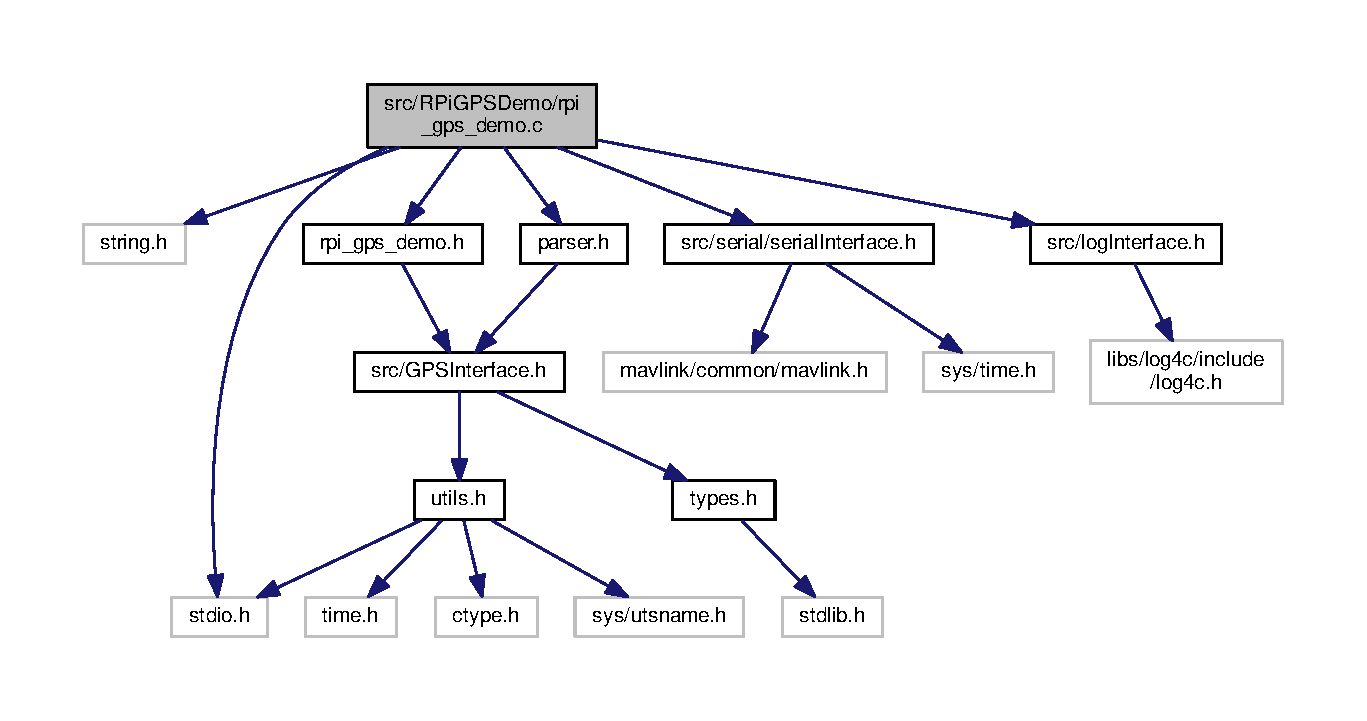
\includegraphics[width=350pt]{rpi__gps__demo_8c__incl}
\end{center}
\end{figure}
\subsection*{Functions}
\begin{DoxyCompactItemize}
\item 
int \hyperlink{rpi__gps__demo_8c_a1cdf9628d4347a87689fda8cffb5a2fb}{get\+G\+P\+S\+Sample\+\_\+\+R\+PI} (\hyperlink{struct_full_g_p_s_data}{Full\+G\+P\+S\+Data} $\ast$samp, \hyperlink{types_8h_af6a258d8f3ee5206d682d799316314b1}{bool} pass\+To\+Log, void $\ast$user\+Data)
\begin{DoxyCompactList}\small\item\em basically gets G\+PS data \end{DoxyCompactList}\end{DoxyCompactItemize}


\subsection{Function Documentation}
\index{rpi\+\_\+gps\+\_\+demo.\+c@{rpi\+\_\+gps\+\_\+demo.\+c}!get\+G\+P\+S\+Sample\+\_\+\+R\+PI@{get\+G\+P\+S\+Sample\+\_\+\+R\+PI}}
\index{get\+G\+P\+S\+Sample\+\_\+\+R\+PI@{get\+G\+P\+S\+Sample\+\_\+\+R\+PI}!rpi\+\_\+gps\+\_\+demo.\+c@{rpi\+\_\+gps\+\_\+demo.\+c}}
\subsubsection[{\texorpdfstring{get\+G\+P\+S\+Sample\+\_\+\+R\+P\+I(\+Full\+G\+P\+S\+Data $\ast$samp, bool pass\+To\+Log, void $\ast$user\+Data)}{getGPSSample_RPI(FullGPSData *samp, bool passToLog, void *userData)}}]{\setlength{\rightskip}{0pt plus 5cm}int get\+G\+P\+S\+Sample\+\_\+\+R\+PI (
\begin{DoxyParamCaption}
\item[{{\bf Full\+G\+P\+S\+Data} $\ast$}]{samp, }
\item[{{\bf bool}}]{pass\+To\+Log, }
\item[{void $\ast$}]{user\+Data}
\end{DoxyParamCaption}
)}\hypertarget{rpi__gps__demo_8c_a1cdf9628d4347a87689fda8cffb5a2fb}{}\label{rpi__gps__demo_8c_a1cdf9628d4347a87689fda8cffb5a2fb}


basically gets G\+PS data 


\begin{DoxyParams}[1]{Parameters}
 & {\em samp} & struct with neccessary data \\
\hline
\mbox{\tt in}  & {\em pass\+To\+Log} & true if we want to log the stuff \\
\hline
\end{DoxyParams}
\begin{DoxyReturn}{Returns}
the ID of the sentence we got on this call. 
\end{DoxyReturn}

\hypertarget{rpi__gps__demo_8d}{}\section{src/\+R\+Pi\+G\+P\+S\+Demo/rpi\+\_\+gps\+\_\+demo.d File Reference}
\label{rpi__gps__demo_8d}\index{src/\+R\+Pi\+G\+P\+S\+Demo/rpi\+\_\+gps\+\_\+demo.\+d@{src/\+R\+Pi\+G\+P\+S\+Demo/rpi\+\_\+gps\+\_\+demo.\+d}}

\hypertarget{rpi__gps__demo_8h}{}\section{src/\+R\+Pi\+G\+P\+S\+Demo/rpi\+\_\+gps\+\_\+demo.h File Reference}
\label{rpi__gps__demo_8h}\index{src/\+R\+Pi\+G\+P\+S\+Demo/rpi\+\_\+gps\+\_\+demo.\+h@{src/\+R\+Pi\+G\+P\+S\+Demo/rpi\+\_\+gps\+\_\+demo.\+h}}
{\ttfamily \#include $<$src/\+G\+P\+S\+Interface.\+h$>$}\\*
Include dependency graph for rpi\+\_\+gps\+\_\+demo.\+h\+:
\nopagebreak
\begin{figure}[H]
\begin{center}
\leavevmode
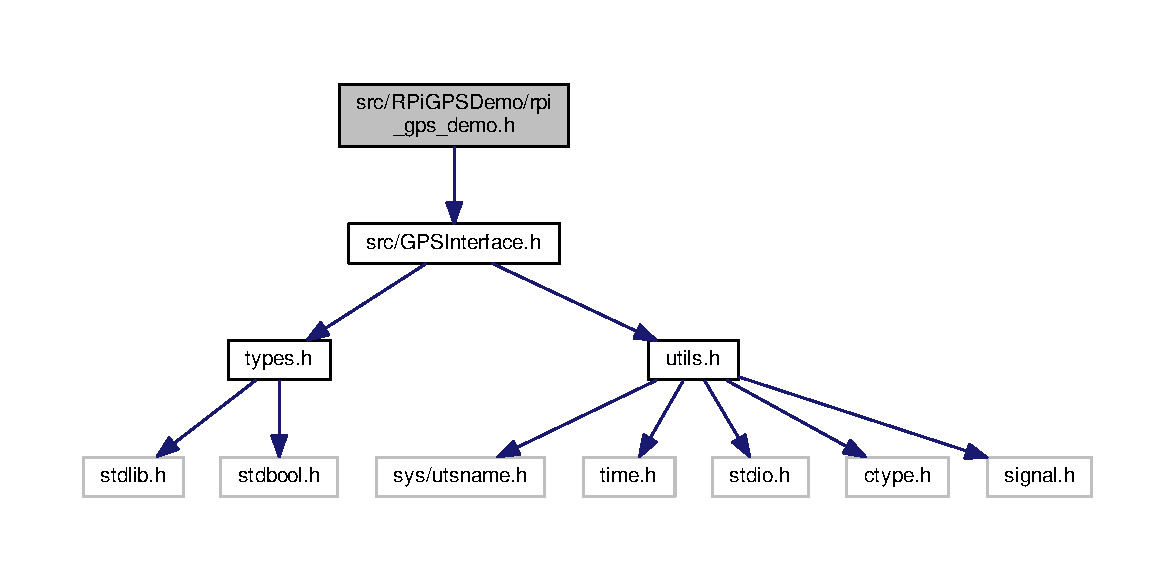
\includegraphics[width=350pt]{rpi__gps__demo_8h__incl}
\end{center}
\end{figure}
This graph shows which files directly or indirectly include this file\+:\nopagebreak
\begin{figure}[H]
\begin{center}
\leavevmode
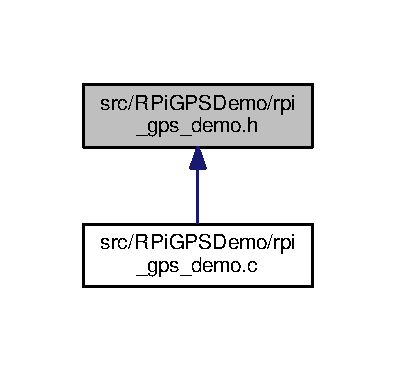
\includegraphics[width=190pt]{rpi__gps__demo_8h__dep__incl}
\end{center}
\end{figure}
\subsection*{Functions}
\begin{DoxyCompactItemize}
\item 
int \hyperlink{rpi__gps__demo_8h_a1cdf9628d4347a87689fda8cffb5a2fb}{get\+G\+P\+S\+Sample\+\_\+\+R\+PI} (\hyperlink{struct_full_g_p_s_data}{Full\+G\+P\+S\+Data} $\ast$samp, bool pass\+To\+Log, void $\ast$user\+Data)
\begin{DoxyCompactList}\small\item\em basically gets G\+PS data \end{DoxyCompactList}\end{DoxyCompactItemize}


\subsection{Function Documentation}
\index{rpi\+\_\+gps\+\_\+demo.\+h@{rpi\+\_\+gps\+\_\+demo.\+h}!get\+G\+P\+S\+Sample\+\_\+\+R\+PI@{get\+G\+P\+S\+Sample\+\_\+\+R\+PI}}
\index{get\+G\+P\+S\+Sample\+\_\+\+R\+PI@{get\+G\+P\+S\+Sample\+\_\+\+R\+PI}!rpi\+\_\+gps\+\_\+demo.\+h@{rpi\+\_\+gps\+\_\+demo.\+h}}
\subsubsection[{\texorpdfstring{get\+G\+P\+S\+Sample\+\_\+\+R\+P\+I(\+Full\+G\+P\+S\+Data $\ast$samp, bool pass\+To\+Log, void $\ast$user\+Data)}{getGPSSample_RPI(FullGPSData *samp, bool passToLog, void *userData)}}]{\setlength{\rightskip}{0pt plus 5cm}int get\+G\+P\+S\+Sample\+\_\+\+R\+PI (
\begin{DoxyParamCaption}
\item[{{\bf Full\+G\+P\+S\+Data} $\ast$}]{samp, }
\item[{bool}]{pass\+To\+Log, }
\item[{void $\ast$}]{user\+Data}
\end{DoxyParamCaption}
)}\hypertarget{rpi__gps__demo_8h_a1cdf9628d4347a87689fda8cffb5a2fb}{}\label{rpi__gps__demo_8h_a1cdf9628d4347a87689fda8cffb5a2fb}


basically gets G\+PS data 


\begin{DoxyParams}[1]{Parameters}
 & {\em samp} & struct with necessary data \\
\hline
\mbox{\tt in}  & {\em pass\+To\+Log} & true if we want to log the stuff \\
\hline
\end{DoxyParams}
\begin{DoxyReturn}{Returns}
the ID of the sentence we got on this call. 
\end{DoxyReturn}

\hypertarget{serial_interface_8c}{}\section{src/serial/serial\+Interface.c File Reference}
\label{serial_interface_8c}\index{src/serial/serial\+Interface.\+c@{src/serial/serial\+Interface.\+c}}
{\ttfamily \#include $<$stdio.\+h$>$}\\*
{\ttfamily \#include $<$string.\+h$>$}\\*
{\ttfamily \#include $<$unistd.\+h$>$}\\*
{\ttfamily \#include $<$fcntl.\+h$>$}\\*
{\ttfamily \#include $<$errno.\+h$>$}\\*
{\ttfamily \#include $<$termios.\+h$>$}\\*
{\ttfamily \#include $<$stdlib.\+h$>$}\\*
{\ttfamily \#include $<$stdbool.\+h$>$}\\*
{\ttfamily \#include \char`\"{}serial\+Interface.\+h\char`\"{}}\\*
{\ttfamily \#include $<$src/log\+Interface.\+h$>$}\\*
Include dependency graph for serial\+Interface.\+c\+:\nopagebreak
\begin{figure}[H]
\begin{center}
\leavevmode
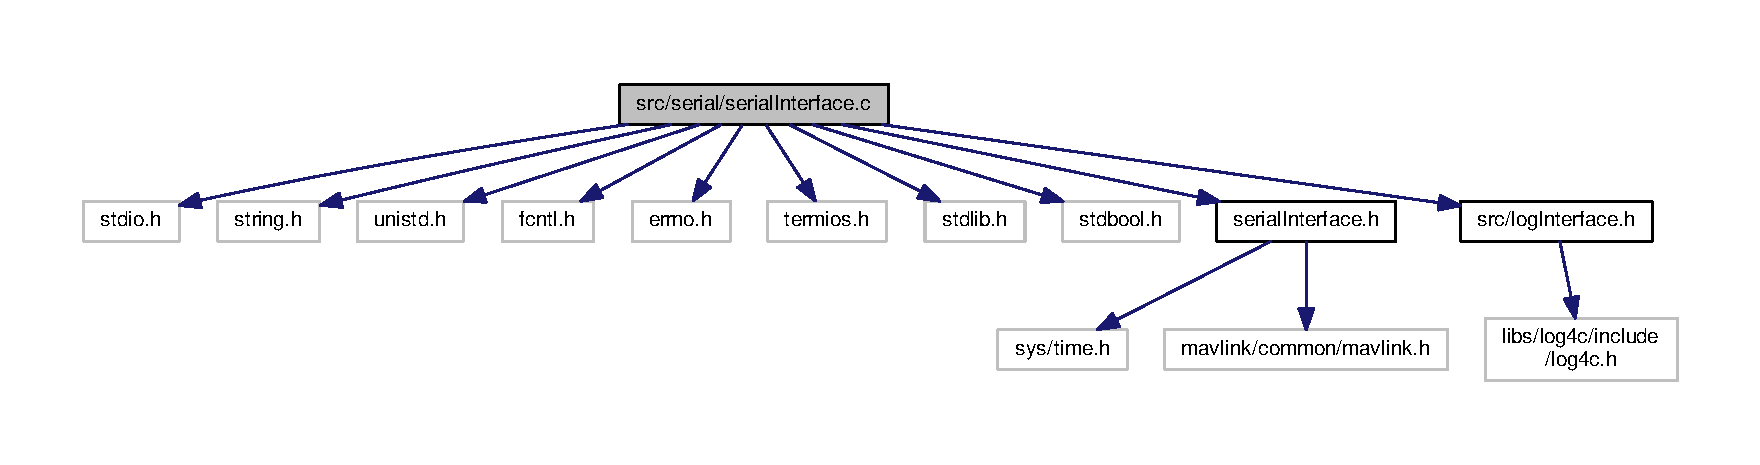
\includegraphics[width=350pt]{serial_interface_8c__incl}
\end{center}
\end{figure}
\subsection*{Functions}
\begin{DoxyCompactItemize}
\item 
int \hyperlink{serial_interface_8c_a0f6c661829d74ed8dc7a5256e6ce7f8a}{open\+\_\+port} (void)
\begin{DoxyCompactList}\small\item\em Opens a port for serial communication. \end{DoxyCompactList}\item 
int \hyperlink{serial_interface_8c_a00c4e146d0eac524e06a95ee43472ff7}{fetch\+\_\+sentence\+\_\+from\+\_\+gps} (int fd, char $\ast$buffer)
\begin{DoxyCompactList}\small\item\em gets one complete N\+M\+EA message from the G\+PS, through the serial port that its on. \end{DoxyCompactList}\item 
void \hyperlink{serial_interface_8c_af0a54246c3213f8835daeebce5e83b0c}{serial\+\_\+start} (const char $\ast$portname)
\begin{DoxyCompactList}\small\item\em Open a serial connection on a specified port. \end{DoxyCompactList}\item 
int \hyperlink{serial_interface_8c_af13dbfaf23b6064cc504fa4bbd81c4ea}{serial\+\_\+read\+\_\+message} (mavlink\+\_\+message\+\_\+t $\ast$message)
\begin{DoxyCompactList}\small\item\em Read one byte at a time from the M\+A\+V\+Link stream on the serial port and populate the mavlink message struct as new bytes arrive. \end{DoxyCompactList}\item 
int \hyperlink{serial_interface_8c_ad9b54717f7dba8da115aa84b94a8c3a2}{usart\+\_\+recv\+\_\+blocking} (int i)
\begin{DoxyCompactList}\small\item\em Blocking read of one byte from the serial port. \end{DoxyCompactList}\item 
int \hyperlink{serial_interface_8c_a363618b75ca75efe669e4a9223e546b9}{serial\+\_\+write\+\_\+message} (const mavlink\+\_\+message\+\_\+t $\ast$message)
\begin{DoxyCompactList}\small\item\em Write a mavlink message to the serial port. \end{DoxyCompactList}\item 
int \hyperlink{serial_interface_8c_a9a535380c30c260dc88af0d5bd48540e}{get\+\_\+time\+\_\+sec} (struct timeval $\ast$tv, struct timezone $\ast$tz)
\begin{DoxyCompactList}\small\item\em Gets the number of seconds and milliseconds since epoch. \end{DoxyCompactList}\item 
int \hyperlink{serial_interface_8c_abe6133ac999c4ce5f06e760aa3ba1827}{get\+\_\+stream\+FD} (void)
\begin{DoxyCompactList}\small\item\em returns stream\+FD. \end{DoxyCompactList}\end{DoxyCompactItemize}
\subsection*{Variables}
\begin{DoxyCompactItemize}
\item 
int \hyperlink{serial_interface_8c_a13869b414e88f5f13a1b32c488e06490}{stream\+FD} = 0
\item 
mavlink\+\_\+status\+\_\+t \hyperlink{serial_interface_8c_acdef7b92239f1e607ef6caa33a16d2ed}{status}
\item 
\hyperlink{types_8h_af6a258d8f3ee5206d682d799316314b1}{bool} \hyperlink{serial_interface_8c_a0c0196118cf8dc54df66d79e21a975c7}{msg\+Received} = \hyperlink{types_8h_af6a258d8f3ee5206d682d799316314b1ae9de385ef6fe9bf3360d1038396b884c}{false}
\item 
volatile float \hyperlink{serial_interface_8c_a6238cddccea71aca0723a82b1411dff6}{seconds}
\item 
struct termios oldtio \hyperlink{serial_interface_8c_abc97f5054a1b45039965e4ee787abc03}{newtio}
\item 
const char $\ast$ \hyperlink{serial_interface_8c_a7a9d64d1e83399aabec1d2b6b3ae6424}{R\+S232\+\_\+\+D\+E\+V\+I\+C\+E\+\_\+const}
\end{DoxyCompactItemize}


\subsection{Function Documentation}
\index{serial\+Interface.\+c@{serial\+Interface.\+c}!fetch\+\_\+sentence\+\_\+from\+\_\+gps@{fetch\+\_\+sentence\+\_\+from\+\_\+gps}}
\index{fetch\+\_\+sentence\+\_\+from\+\_\+gps@{fetch\+\_\+sentence\+\_\+from\+\_\+gps}!serial\+Interface.\+c@{serial\+Interface.\+c}}
\subsubsection[{\texorpdfstring{fetch\+\_\+sentence\+\_\+from\+\_\+gps(int fd, char $\ast$buffer)}{fetch_sentence_from_gps(int fd, char *buffer)}}]{\setlength{\rightskip}{0pt plus 5cm}int fetch\+\_\+sentence\+\_\+from\+\_\+gps (
\begin{DoxyParamCaption}
\item[{int}]{fd, }
\item[{char $\ast$}]{buffer}
\end{DoxyParamCaption}
)}\hypertarget{serial_interface_8c_a00c4e146d0eac524e06a95ee43472ff7}{}\label{serial_interface_8c_a00c4e146d0eac524e06a95ee43472ff7}


gets one complete N\+M\+EA message from the G\+PS, through the serial port that its on. 


\begin{DoxyParams}[1]{Parameters}
\mbox{\tt in}  & {\em fd} & the file descriptor of serial port used for communication with the G\+PS \\
\hline
 & {\em buffer} & the string buffer that the message will be written to. \\
\hline
\end{DoxyParams}
\begin{DoxyReturn}{Returns}
returns the number of characters that were read for this N\+M\+EA sentence. 
\end{DoxyReturn}
\index{serial\+Interface.\+c@{serial\+Interface.\+c}!get\+\_\+stream\+FD@{get\+\_\+stream\+FD}}
\index{get\+\_\+stream\+FD@{get\+\_\+stream\+FD}!serial\+Interface.\+c@{serial\+Interface.\+c}}
\subsubsection[{\texorpdfstring{get\+\_\+stream\+F\+D(void)}{get_streamFD(void)}}]{\setlength{\rightskip}{0pt plus 5cm}int get\+\_\+stream\+FD (
\begin{DoxyParamCaption}
\item[{void}]{}
\end{DoxyParamCaption}
)}\hypertarget{serial_interface_8c_abe6133ac999c4ce5f06e760aa3ba1827}{}\label{serial_interface_8c_abe6133ac999c4ce5f06e760aa3ba1827}


returns stream\+FD. 

\index{serial\+Interface.\+c@{serial\+Interface.\+c}!get\+\_\+time\+\_\+sec@{get\+\_\+time\+\_\+sec}}
\index{get\+\_\+time\+\_\+sec@{get\+\_\+time\+\_\+sec}!serial\+Interface.\+c@{serial\+Interface.\+c}}
\subsubsection[{\texorpdfstring{get\+\_\+time\+\_\+sec(struct timeval $\ast$tv, struct timezone $\ast$tz)}{get_time_sec(struct timeval *tv, struct timezone *tz)}}]{\setlength{\rightskip}{0pt plus 5cm}int get\+\_\+time\+\_\+sec (
\begin{DoxyParamCaption}
\item[{struct timeval $\ast$}]{tv, }
\item[{struct timezone $\ast$}]{tz}
\end{DoxyParamCaption}
)}\hypertarget{serial_interface_8c_a9a535380c30c260dc88af0d5bd48540e}{}\label{serial_interface_8c_a9a535380c30c260dc88af0d5bd48540e}


Gets the number of seconds and milliseconds since epoch. 


\begin{DoxyParams}{Parameters}
{\em tv} & the timeval struct (sys/time.\+h) \\
\hline
{\em tz} & the timezone struct\\
\hline
\end{DoxyParams}
\begin{DoxyReturn}{Returns}
0 for successful write to structs and -\/1 for failure. 
\end{DoxyReturn}
\index{serial\+Interface.\+c@{serial\+Interface.\+c}!open\+\_\+port@{open\+\_\+port}}
\index{open\+\_\+port@{open\+\_\+port}!serial\+Interface.\+c@{serial\+Interface.\+c}}
\subsubsection[{\texorpdfstring{open\+\_\+port(void)}{open_port(void)}}]{\setlength{\rightskip}{0pt plus 5cm}int open\+\_\+port (
\begin{DoxyParamCaption}
\item[{void}]{}
\end{DoxyParamCaption}
)}\hypertarget{serial_interface_8c_a0f6c661829d74ed8dc7a5256e6ce7f8a}{}\label{serial_interface_8c_a0f6c661829d74ed8dc7a5256e6ce7f8a}


Opens a port for serial communication. 

\begin{DoxyReturn}{Returns}
returns an int that\textquotesingle{}s the file descriptor of the opened port. 
\end{DoxyReturn}
\index{serial\+Interface.\+c@{serial\+Interface.\+c}!serial\+\_\+read\+\_\+message@{serial\+\_\+read\+\_\+message}}
\index{serial\+\_\+read\+\_\+message@{serial\+\_\+read\+\_\+message}!serial\+Interface.\+c@{serial\+Interface.\+c}}
\subsubsection[{\texorpdfstring{serial\+\_\+read\+\_\+message(mavlink\+\_\+message\+\_\+t $\ast$message)}{serial_read_message(mavlink_message_t *message)}}]{\setlength{\rightskip}{0pt plus 5cm}int serial\+\_\+read\+\_\+message (
\begin{DoxyParamCaption}
\item[{mavlink\+\_\+message\+\_\+t $\ast$}]{message}
\end{DoxyParamCaption}
)}\hypertarget{serial_interface_8c_af13dbfaf23b6064cc504fa4bbd81c4ea}{}\label{serial_interface_8c_af13dbfaf23b6064cc504fa4bbd81c4ea}


Read one byte at a time from the M\+A\+V\+Link stream on the serial port and populate the mavlink message struct as new bytes arrive. 


\begin{DoxyParams}{Parameters}
{\em message} & The M\+A\+V\+Link message struct which is populated with the parse data that\textquotesingle{}s received from the serial port.\\
\hline
\end{DoxyParams}
\begin{DoxyReturn}{Returns}
1 if a complete M\+A\+V\+Link message could be read, 0 otherwise. 
\end{DoxyReturn}
\index{serial\+Interface.\+c@{serial\+Interface.\+c}!serial\+\_\+start@{serial\+\_\+start}}
\index{serial\+\_\+start@{serial\+\_\+start}!serial\+Interface.\+c@{serial\+Interface.\+c}}
\subsubsection[{\texorpdfstring{serial\+\_\+start(const char $\ast$portname)}{serial_start(const char *portname)}}]{\setlength{\rightskip}{0pt plus 5cm}void serial\+\_\+start (
\begin{DoxyParamCaption}
\item[{const char $\ast$}]{portname}
\end{DoxyParamCaption}
)}\hypertarget{serial_interface_8c_af0a54246c3213f8835daeebce5e83b0c}{}\label{serial_interface_8c_af0a54246c3213f8835daeebce5e83b0c}


Open a serial connection on a specified port. 


\begin{DoxyParams}[1]{Parameters}
\mbox{\tt in}  & {\em portname} & The name of the serial port \\
\hline
\end{DoxyParams}
\index{serial\+Interface.\+c@{serial\+Interface.\+c}!serial\+\_\+write\+\_\+message@{serial\+\_\+write\+\_\+message}}
\index{serial\+\_\+write\+\_\+message@{serial\+\_\+write\+\_\+message}!serial\+Interface.\+c@{serial\+Interface.\+c}}
\subsubsection[{\texorpdfstring{serial\+\_\+write\+\_\+message(const mavlink\+\_\+message\+\_\+t $\ast$message)}{serial_write_message(const mavlink_message_t *message)}}]{\setlength{\rightskip}{0pt plus 5cm}int serial\+\_\+write\+\_\+message (
\begin{DoxyParamCaption}
\item[{const mavlink\+\_\+message\+\_\+t $\ast$}]{message}
\end{DoxyParamCaption}
)}\hypertarget{serial_interface_8c_a363618b75ca75efe669e4a9223e546b9}{}\label{serial_interface_8c_a363618b75ca75efe669e4a9223e546b9}


Write a mavlink message to the serial port. 


\begin{DoxyParams}[1]{Parameters}
\mbox{\tt in}  & {\em message} & The M\+A\+V\+Link message to be written.\\
\hline
\end{DoxyParams}
\begin{DoxyReturn}{Returns}
The number of bytes written to the serial port (the size of the message). 
\end{DoxyReturn}
\index{serial\+Interface.\+c@{serial\+Interface.\+c}!usart\+\_\+recv\+\_\+blocking@{usart\+\_\+recv\+\_\+blocking}}
\index{usart\+\_\+recv\+\_\+blocking@{usart\+\_\+recv\+\_\+blocking}!serial\+Interface.\+c@{serial\+Interface.\+c}}
\subsubsection[{\texorpdfstring{usart\+\_\+recv\+\_\+blocking(int i)}{usart_recv_blocking(int i)}}]{\setlength{\rightskip}{0pt plus 5cm}int usart\+\_\+recv\+\_\+blocking (
\begin{DoxyParamCaption}
\item[{int}]{i}
\end{DoxyParamCaption}
)}\hypertarget{serial_interface_8c_ad9b54717f7dba8da115aa84b94a8c3a2}{}\label{serial_interface_8c_ad9b54717f7dba8da115aa84b94a8c3a2}


Blocking read of one byte from the serial port. 


\begin{DoxyParams}[1]{Parameters}
\mbox{\tt in}  & {\em i} & Unused\\
\hline
\end{DoxyParams}
\begin{DoxyReturn}{Returns}
The read byte. 
\end{DoxyReturn}


\subsection{Variable Documentation}
\index{serial\+Interface.\+c@{serial\+Interface.\+c}!msg\+Received@{msg\+Received}}
\index{msg\+Received@{msg\+Received}!serial\+Interface.\+c@{serial\+Interface.\+c}}
\subsubsection[{\texorpdfstring{msg\+Received}{msgReceived}}]{\setlength{\rightskip}{0pt plus 5cm}{\bf bool} msg\+Received = {\bf false}}\hypertarget{serial_interface_8c_a0c0196118cf8dc54df66d79e21a975c7}{}\label{serial_interface_8c_a0c0196118cf8dc54df66d79e21a975c7}
\index{serial\+Interface.\+c@{serial\+Interface.\+c}!newtio@{newtio}}
\index{newtio@{newtio}!serial\+Interface.\+c@{serial\+Interface.\+c}}
\subsubsection[{\texorpdfstring{newtio}{newtio}}]{\setlength{\rightskip}{0pt plus 5cm}struct termios oldtio newtio}\hypertarget{serial_interface_8c_abc97f5054a1b45039965e4ee787abc03}{}\label{serial_interface_8c_abc97f5054a1b45039965e4ee787abc03}
\index{serial\+Interface.\+c@{serial\+Interface.\+c}!R\+S232\+\_\+\+D\+E\+V\+I\+C\+E\+\_\+const@{R\+S232\+\_\+\+D\+E\+V\+I\+C\+E\+\_\+const}}
\index{R\+S232\+\_\+\+D\+E\+V\+I\+C\+E\+\_\+const@{R\+S232\+\_\+\+D\+E\+V\+I\+C\+E\+\_\+const}!serial\+Interface.\+c@{serial\+Interface.\+c}}
\subsubsection[{\texorpdfstring{R\+S232\+\_\+\+D\+E\+V\+I\+C\+E\+\_\+const}{RS232_DEVICE_const}}]{\setlength{\rightskip}{0pt plus 5cm}const char$\ast$ R\+S232\+\_\+\+D\+E\+V\+I\+C\+E\+\_\+const}\hypertarget{serial_interface_8c_a7a9d64d1e83399aabec1d2b6b3ae6424}{}\label{serial_interface_8c_a7a9d64d1e83399aabec1d2b6b3ae6424}
\index{serial\+Interface.\+c@{serial\+Interface.\+c}!seconds@{seconds}}
\index{seconds@{seconds}!serial\+Interface.\+c@{serial\+Interface.\+c}}
\subsubsection[{\texorpdfstring{seconds}{seconds}}]{\setlength{\rightskip}{0pt plus 5cm}volatile float seconds}\hypertarget{serial_interface_8c_a6238cddccea71aca0723a82b1411dff6}{}\label{serial_interface_8c_a6238cddccea71aca0723a82b1411dff6}
\index{serial\+Interface.\+c@{serial\+Interface.\+c}!status@{status}}
\index{status@{status}!serial\+Interface.\+c@{serial\+Interface.\+c}}
\subsubsection[{\texorpdfstring{status}{status}}]{\setlength{\rightskip}{0pt plus 5cm}mavlink\+\_\+status\+\_\+t status}\hypertarget{serial_interface_8c_acdef7b92239f1e607ef6caa33a16d2ed}{}\label{serial_interface_8c_acdef7b92239f1e607ef6caa33a16d2ed}
\index{serial\+Interface.\+c@{serial\+Interface.\+c}!stream\+FD@{stream\+FD}}
\index{stream\+FD@{stream\+FD}!serial\+Interface.\+c@{serial\+Interface.\+c}}
\subsubsection[{\texorpdfstring{stream\+FD}{streamFD}}]{\setlength{\rightskip}{0pt plus 5cm}int stream\+FD = 0}\hypertarget{serial_interface_8c_a13869b414e88f5f13a1b32c488e06490}{}\label{serial_interface_8c_a13869b414e88f5f13a1b32c488e06490}
the file descriptor of the port that will be opened using \hyperlink{serial_interface_8h_a0f6c661829d74ed8dc7a5256e6ce7f8a}{open\+\_\+port()}. 
\hypertarget{serial_interface_8d}{}\section{src/serial/serial\+Interface.d File Reference}
\label{serial_interface_8d}\index{src/serial/serial\+Interface.\+d@{src/serial/serial\+Interface.\+d}}

\hypertarget{serial_interface_8h}{}\section{src/serial/serial\+Interface.h File Reference}
\label{serial_interface_8h}\index{src/serial/serial\+Interface.\+h@{src/serial/serial\+Interface.\+h}}
{\ttfamily \#include $<$sys/time.\+h$>$}\\*
{\ttfamily \#include $<$mavlink/common/mavlink.\+h$>$}\\*
Include dependency graph for serial\+Interface.\+h\+:
\nopagebreak
\begin{figure}[H]
\begin{center}
\leavevmode
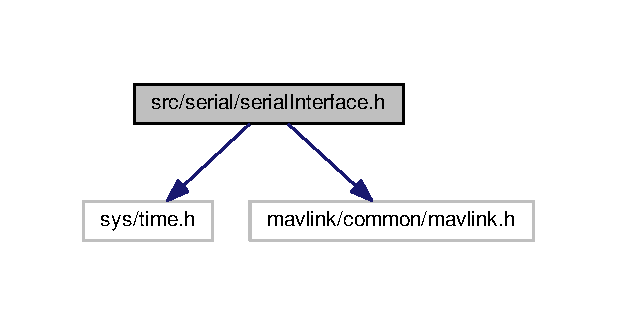
\includegraphics[width=296pt]{serial_interface_8h__incl}
\end{center}
\end{figure}
This graph shows which files directly or indirectly include this file\+:
\nopagebreak
\begin{figure}[H]
\begin{center}
\leavevmode
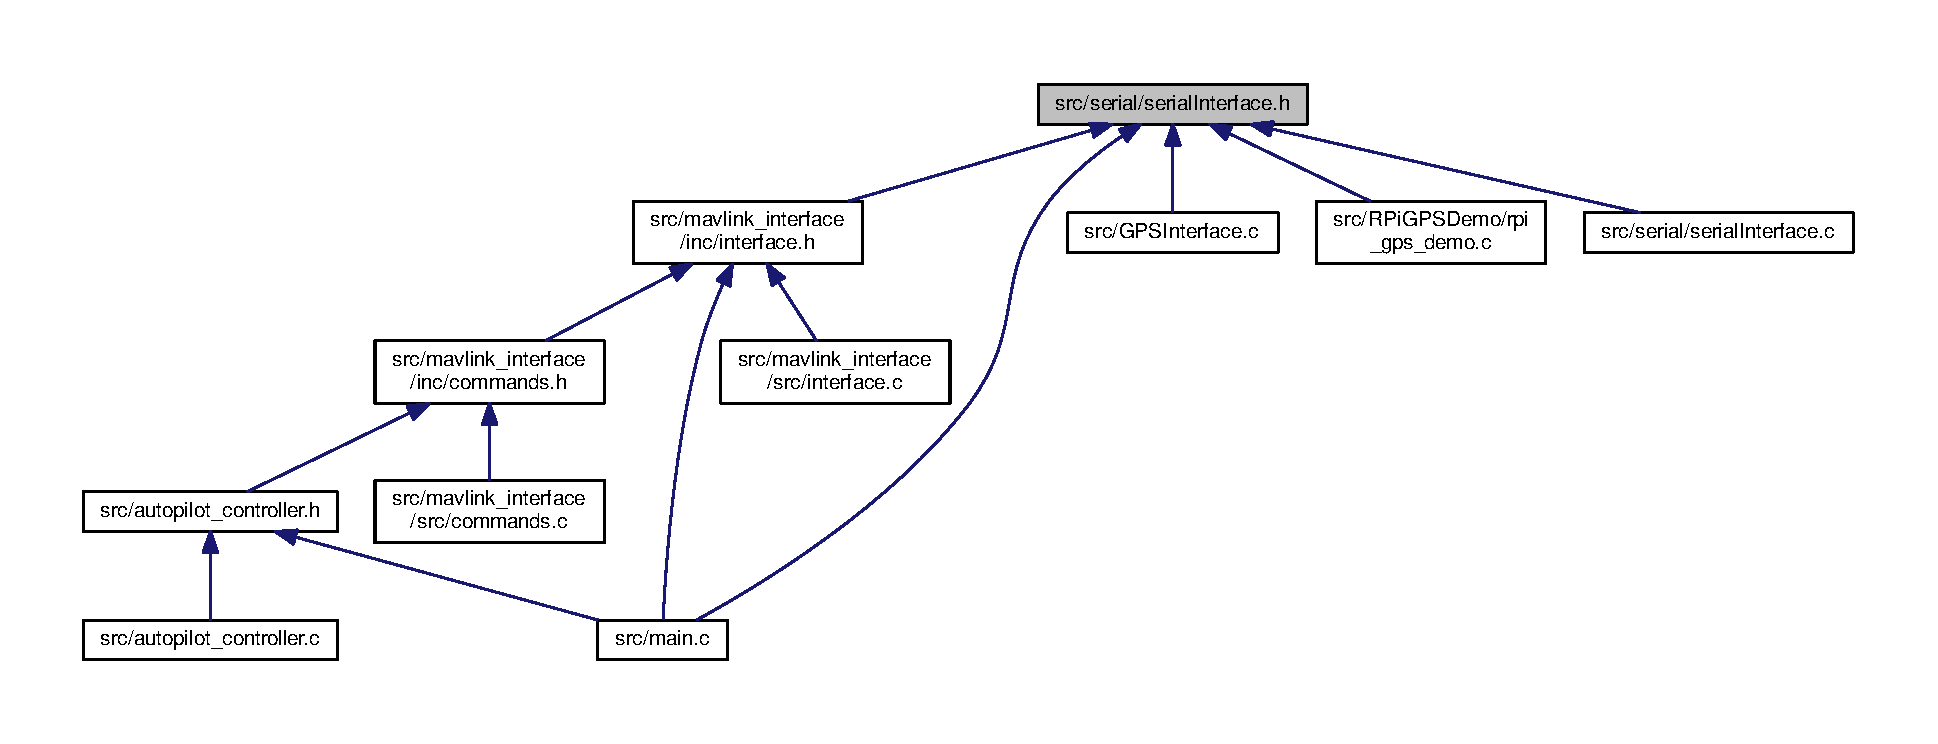
\includegraphics[width=350pt]{serial_interface_8h__dep__incl}
\end{center}
\end{figure}
\subsection*{Macros}
\begin{DoxyCompactItemize}
\item 
\#define \hyperlink{serial_interface_8h_a2350115553c1fe0a7bc14e6a7ec6a225}{U\+S\+A\+R\+T3}~3
\item 
\#define \hyperlink{serial_interface_8h_a734bbab06e1a9fd2e5522db0221ff6e3}{B\+A\+U\+D\+R\+A\+TE}~B57600
\item 
\#define \hyperlink{serial_interface_8h_ac1b2a6fd5fee10751f9de6082a0fc138}{R\+S232\+\_\+\+D\+E\+V\+I\+CE}~\char`\"{}dev/tty\+U\+S\+B0\char`\"{}
\end{DoxyCompactItemize}
\subsection*{Functions}
\begin{DoxyCompactItemize}
\item 
int \hyperlink{serial_interface_8h_abe6133ac999c4ce5f06e760aa3ba1827}{get\+\_\+stream\+FD} (void)
\begin{DoxyCompactList}\small\item\em returns stream\+FD. \end{DoxyCompactList}\item 
int \hyperlink{serial_interface_8h_a0f6c661829d74ed8dc7a5256e6ce7f8a}{open\+\_\+port} (void)
\begin{DoxyCompactList}\small\item\em Opens a port for serial communication. \end{DoxyCompactList}\item 
int \hyperlink{serial_interface_8h_a00c4e146d0eac524e06a95ee43472ff7}{fetch\+\_\+sentence\+\_\+from\+\_\+gps} (int fd, char $\ast$buffer)
\begin{DoxyCompactList}\small\item\em gets one complete N\+M\+EA message from the G\+PS, through the serial port that its on. \end{DoxyCompactList}\item 
int \hyperlink{serial_interface_8h_ad9b54717f7dba8da115aa84b94a8c3a2}{usart\+\_\+recv\+\_\+blocking} (int i)
\begin{DoxyCompactList}\small\item\em Blocking read of one byte from the serial port. \end{DoxyCompactList}\item 
void \hyperlink{serial_interface_8h_af0a54246c3213f8835daeebce5e83b0c}{serial\+\_\+start} (const char $\ast$portname)
\begin{DoxyCompactList}\small\item\em Open a serial connection on a specified port. \end{DoxyCompactList}\item 
int \hyperlink{serial_interface_8h_af13dbfaf23b6064cc504fa4bbd81c4ea}{serial\+\_\+read\+\_\+message} (mavlink\+\_\+message\+\_\+t $\ast$message)
\begin{DoxyCompactList}\small\item\em Read one byte at a time from the M\+A\+V\+Link stream on the serial port and populate the mavlink message struct as new bytes arrive. \end{DoxyCompactList}\item 
int \hyperlink{serial_interface_8h_a363618b75ca75efe669e4a9223e546b9}{serial\+\_\+write\+\_\+message} (const mavlink\+\_\+message\+\_\+t $\ast$message)
\begin{DoxyCompactList}\small\item\em Write a mavlink message to the serial port. \end{DoxyCompactList}\item 
int \hyperlink{serial_interface_8h_a9a535380c30c260dc88af0d5bd48540e}{get\+\_\+time\+\_\+sec} (struct timeval $\ast$tv, struct timezone $\ast$tz)
\begin{DoxyCompactList}\small\item\em Gets the nubmer of seconds and milliseconds since epoch. \end{DoxyCompactList}\end{DoxyCompactItemize}
\subsection*{Variables}
\begin{DoxyCompactItemize}
\item 
int \hyperlink{serial_interface_8h_a13869b414e88f5f13a1b32c488e06490}{stream\+FD}
\item 
const char $\ast$ \hyperlink{serial_interface_8h_a7a9d64d1e83399aabec1d2b6b3ae6424}{R\+S232\+\_\+\+D\+E\+V\+I\+C\+E\+\_\+const}
\end{DoxyCompactItemize}


\subsection{Macro Definition Documentation}
\index{serial\+Interface.\+h@{serial\+Interface.\+h}!B\+A\+U\+D\+R\+A\+TE@{B\+A\+U\+D\+R\+A\+TE}}
\index{B\+A\+U\+D\+R\+A\+TE@{B\+A\+U\+D\+R\+A\+TE}!serial\+Interface.\+h@{serial\+Interface.\+h}}
\subsubsection[{\texorpdfstring{B\+A\+U\+D\+R\+A\+TE}{BAUDRATE}}]{\setlength{\rightskip}{0pt plus 5cm}\#define B\+A\+U\+D\+R\+A\+TE~B57600}\hypertarget{serial_interface_8h_a734bbab06e1a9fd2e5522db0221ff6e3}{}\label{serial_interface_8h_a734bbab06e1a9fd2e5522db0221ff6e3}
\index{serial\+Interface.\+h@{serial\+Interface.\+h}!R\+S232\+\_\+\+D\+E\+V\+I\+CE@{R\+S232\+\_\+\+D\+E\+V\+I\+CE}}
\index{R\+S232\+\_\+\+D\+E\+V\+I\+CE@{R\+S232\+\_\+\+D\+E\+V\+I\+CE}!serial\+Interface.\+h@{serial\+Interface.\+h}}
\subsubsection[{\texorpdfstring{R\+S232\+\_\+\+D\+E\+V\+I\+CE}{RS232_DEVICE}}]{\setlength{\rightskip}{0pt plus 5cm}\#define R\+S232\+\_\+\+D\+E\+V\+I\+CE~\char`\"{}dev/tty\+U\+S\+B0\char`\"{}}\hypertarget{serial_interface_8h_ac1b2a6fd5fee10751f9de6082a0fc138}{}\label{serial_interface_8h_ac1b2a6fd5fee10751f9de6082a0fc138}
\index{serial\+Interface.\+h@{serial\+Interface.\+h}!U\+S\+A\+R\+T3@{U\+S\+A\+R\+T3}}
\index{U\+S\+A\+R\+T3@{U\+S\+A\+R\+T3}!serial\+Interface.\+h@{serial\+Interface.\+h}}
\subsubsection[{\texorpdfstring{U\+S\+A\+R\+T3}{USART3}}]{\setlength{\rightskip}{0pt plus 5cm}\#define U\+S\+A\+R\+T3~3}\hypertarget{serial_interface_8h_a2350115553c1fe0a7bc14e6a7ec6a225}{}\label{serial_interface_8h_a2350115553c1fe0a7bc14e6a7ec6a225}


\subsection{Function Documentation}
\index{serial\+Interface.\+h@{serial\+Interface.\+h}!fetch\+\_\+sentence\+\_\+from\+\_\+gps@{fetch\+\_\+sentence\+\_\+from\+\_\+gps}}
\index{fetch\+\_\+sentence\+\_\+from\+\_\+gps@{fetch\+\_\+sentence\+\_\+from\+\_\+gps}!serial\+Interface.\+h@{serial\+Interface.\+h}}
\subsubsection[{\texorpdfstring{fetch\+\_\+sentence\+\_\+from\+\_\+gps(int fd, char $\ast$buffer)}{fetch_sentence_from_gps(int fd, char *buffer)}}]{\setlength{\rightskip}{0pt plus 5cm}int fetch\+\_\+sentence\+\_\+from\+\_\+gps (
\begin{DoxyParamCaption}
\item[{int}]{fd, }
\item[{char $\ast$}]{buffer}
\end{DoxyParamCaption}
)}\hypertarget{serial_interface_8h_a00c4e146d0eac524e06a95ee43472ff7}{}\label{serial_interface_8h_a00c4e146d0eac524e06a95ee43472ff7}


gets one complete N\+M\+EA message from the G\+PS, through the serial port that its on. 


\begin{DoxyParams}[1]{Parameters}
\mbox{\tt in}  & {\em fd} & the file descriptor of serial port used for communication with the G\+PS \\
\hline
 & {\em buffer} & the string buffer that the message will be written to. \\
\hline
\end{DoxyParams}
\begin{DoxyReturn}{Returns}
returns the number of charachters that were read for this N\+M\+EA sentence. 
\end{DoxyReturn}
\index{serial\+Interface.\+h@{serial\+Interface.\+h}!get\+\_\+stream\+FD@{get\+\_\+stream\+FD}}
\index{get\+\_\+stream\+FD@{get\+\_\+stream\+FD}!serial\+Interface.\+h@{serial\+Interface.\+h}}
\subsubsection[{\texorpdfstring{get\+\_\+stream\+F\+D(void)}{get_streamFD(void)}}]{\setlength{\rightskip}{0pt plus 5cm}int get\+\_\+stream\+FD (
\begin{DoxyParamCaption}
\item[{void}]{}
\end{DoxyParamCaption}
)}\hypertarget{serial_interface_8h_abe6133ac999c4ce5f06e760aa3ba1827}{}\label{serial_interface_8h_abe6133ac999c4ce5f06e760aa3ba1827}


returns stream\+FD. 

\index{serial\+Interface.\+h@{serial\+Interface.\+h}!get\+\_\+time\+\_\+sec@{get\+\_\+time\+\_\+sec}}
\index{get\+\_\+time\+\_\+sec@{get\+\_\+time\+\_\+sec}!serial\+Interface.\+h@{serial\+Interface.\+h}}
\subsubsection[{\texorpdfstring{get\+\_\+time\+\_\+sec(struct timeval $\ast$tv, struct timezone $\ast$tz)}{get_time_sec(struct timeval *tv, struct timezone *tz)}}]{\setlength{\rightskip}{0pt plus 5cm}int get\+\_\+time\+\_\+sec (
\begin{DoxyParamCaption}
\item[{struct timeval $\ast$}]{tv, }
\item[{struct timezone $\ast$}]{tz}
\end{DoxyParamCaption}
)}\hypertarget{serial_interface_8h_a9a535380c30c260dc88af0d5bd48540e}{}\label{serial_interface_8h_a9a535380c30c260dc88af0d5bd48540e}


Gets the nubmer of seconds and milliseconds since epoch. 


\begin{DoxyParams}{Parameters}
{\em tv} & the timeval struct (sys/time.\+h) \\
\hline
{\em tz} & the timezone struct\\
\hline
\end{DoxyParams}
\begin{DoxyReturn}{Returns}
0 for successful write to structs and -\/1 for failure. 
\end{DoxyReturn}
\index{serial\+Interface.\+h@{serial\+Interface.\+h}!open\+\_\+port@{open\+\_\+port}}
\index{open\+\_\+port@{open\+\_\+port}!serial\+Interface.\+h@{serial\+Interface.\+h}}
\subsubsection[{\texorpdfstring{open\+\_\+port(void)}{open_port(void)}}]{\setlength{\rightskip}{0pt plus 5cm}int open\+\_\+port (
\begin{DoxyParamCaption}
\item[{void}]{}
\end{DoxyParamCaption}
)}\hypertarget{serial_interface_8h_a0f6c661829d74ed8dc7a5256e6ce7f8a}{}\label{serial_interface_8h_a0f6c661829d74ed8dc7a5256e6ce7f8a}


Opens a port for serial communication. 

\begin{DoxyReturn}{Returns}
returns an int that\textquotesingle{}s the file descriptor of the opened port. 
\end{DoxyReturn}
\index{serial\+Interface.\+h@{serial\+Interface.\+h}!serial\+\_\+read\+\_\+message@{serial\+\_\+read\+\_\+message}}
\index{serial\+\_\+read\+\_\+message@{serial\+\_\+read\+\_\+message}!serial\+Interface.\+h@{serial\+Interface.\+h}}
\subsubsection[{\texorpdfstring{serial\+\_\+read\+\_\+message(mavlink\+\_\+message\+\_\+t $\ast$message)}{serial_read_message(mavlink_message_t *message)}}]{\setlength{\rightskip}{0pt plus 5cm}int serial\+\_\+read\+\_\+message (
\begin{DoxyParamCaption}
\item[{mavlink\+\_\+message\+\_\+t $\ast$}]{message}
\end{DoxyParamCaption}
)}\hypertarget{serial_interface_8h_af13dbfaf23b6064cc504fa4bbd81c4ea}{}\label{serial_interface_8h_af13dbfaf23b6064cc504fa4bbd81c4ea}


Read one byte at a time from the M\+A\+V\+Link stream on the serial port and populate the mavlink message struct as new bytes arrive. 


\begin{DoxyParams}{Parameters}
{\em message} & The M\+A\+V\+Link message struct which is populated with the parse data that\textquotesingle{}s received fom the serial port.\\
\hline
\end{DoxyParams}
\begin{DoxyReturn}{Returns}
1 if a complete M\+A\+V\+Link message could be read, 0 otherwise. 
\end{DoxyReturn}
\index{serial\+Interface.\+h@{serial\+Interface.\+h}!serial\+\_\+start@{serial\+\_\+start}}
\index{serial\+\_\+start@{serial\+\_\+start}!serial\+Interface.\+h@{serial\+Interface.\+h}}
\subsubsection[{\texorpdfstring{serial\+\_\+start(const char $\ast$portname)}{serial_start(const char *portname)}}]{\setlength{\rightskip}{0pt plus 5cm}void serial\+\_\+start (
\begin{DoxyParamCaption}
\item[{const char $\ast$}]{portname}
\end{DoxyParamCaption}
)}\hypertarget{serial_interface_8h_af0a54246c3213f8835daeebce5e83b0c}{}\label{serial_interface_8h_af0a54246c3213f8835daeebce5e83b0c}


Open a serial connection on a specified port. 


\begin{DoxyParams}[1]{Parameters}
\mbox{\tt in}  & {\em portname} & The name of the serial port \\
\hline
\end{DoxyParams}
\index{serial\+Interface.\+h@{serial\+Interface.\+h}!serial\+\_\+write\+\_\+message@{serial\+\_\+write\+\_\+message}}
\index{serial\+\_\+write\+\_\+message@{serial\+\_\+write\+\_\+message}!serial\+Interface.\+h@{serial\+Interface.\+h}}
\subsubsection[{\texorpdfstring{serial\+\_\+write\+\_\+message(const mavlink\+\_\+message\+\_\+t $\ast$message)}{serial_write_message(const mavlink_message_t *message)}}]{\setlength{\rightskip}{0pt plus 5cm}int serial\+\_\+write\+\_\+message (
\begin{DoxyParamCaption}
\item[{const mavlink\+\_\+message\+\_\+t $\ast$}]{message}
\end{DoxyParamCaption}
)}\hypertarget{serial_interface_8h_a363618b75ca75efe669e4a9223e546b9}{}\label{serial_interface_8h_a363618b75ca75efe669e4a9223e546b9}


Write a mavlink message to the serial port. 


\begin{DoxyParams}[1]{Parameters}
\mbox{\tt in}  & {\em message} & The M\+A\+V\+Link message to be written.\\
\hline
\end{DoxyParams}
\begin{DoxyReturn}{Returns}
The number of bytes written to the serial port (the size of the message). 
\end{DoxyReturn}
\index{serial\+Interface.\+h@{serial\+Interface.\+h}!usart\+\_\+recv\+\_\+blocking@{usart\+\_\+recv\+\_\+blocking}}
\index{usart\+\_\+recv\+\_\+blocking@{usart\+\_\+recv\+\_\+blocking}!serial\+Interface.\+h@{serial\+Interface.\+h}}
\subsubsection[{\texorpdfstring{usart\+\_\+recv\+\_\+blocking(int i)}{usart_recv_blocking(int i)}}]{\setlength{\rightskip}{0pt plus 5cm}int usart\+\_\+recv\+\_\+blocking (
\begin{DoxyParamCaption}
\item[{int}]{i}
\end{DoxyParamCaption}
)}\hypertarget{serial_interface_8h_ad9b54717f7dba8da115aa84b94a8c3a2}{}\label{serial_interface_8h_ad9b54717f7dba8da115aa84b94a8c3a2}


Blocking read of one byte from the serial port. 


\begin{DoxyParams}[1]{Parameters}
\mbox{\tt in}  & {\em i} & Unused\\
\hline
\end{DoxyParams}
\begin{DoxyReturn}{Returns}
The read byte. 
\end{DoxyReturn}


\subsection{Variable Documentation}
\index{serial\+Interface.\+h@{serial\+Interface.\+h}!R\+S232\+\_\+\+D\+E\+V\+I\+C\+E\+\_\+const@{R\+S232\+\_\+\+D\+E\+V\+I\+C\+E\+\_\+const}}
\index{R\+S232\+\_\+\+D\+E\+V\+I\+C\+E\+\_\+const@{R\+S232\+\_\+\+D\+E\+V\+I\+C\+E\+\_\+const}!serial\+Interface.\+h@{serial\+Interface.\+h}}
\subsubsection[{\texorpdfstring{R\+S232\+\_\+\+D\+E\+V\+I\+C\+E\+\_\+const}{RS232_DEVICE_const}}]{\setlength{\rightskip}{0pt plus 5cm}const char$\ast$ R\+S232\+\_\+\+D\+E\+V\+I\+C\+E\+\_\+const}\hypertarget{serial_interface_8h_a7a9d64d1e83399aabec1d2b6b3ae6424}{}\label{serial_interface_8h_a7a9d64d1e83399aabec1d2b6b3ae6424}
\index{serial\+Interface.\+h@{serial\+Interface.\+h}!stream\+FD@{stream\+FD}}
\index{stream\+FD@{stream\+FD}!serial\+Interface.\+h@{serial\+Interface.\+h}}
\subsubsection[{\texorpdfstring{stream\+FD}{streamFD}}]{\setlength{\rightskip}{0pt plus 5cm}int stream\+FD}\hypertarget{serial_interface_8h_a13869b414e88f5f13a1b32c488e06490}{}\label{serial_interface_8h_a13869b414e88f5f13a1b32c488e06490}
the file descriptor of the port that will be opened using \hyperlink{serial_interface_8h_a0f6c661829d74ed8dc7a5256e6ce7f8a}{open\+\_\+port()}. 
\hypertarget{types_8h}{}\section{src/types.h File Reference}
\label{types_8h}\index{src/types.\+h@{src/types.\+h}}
{\ttfamily \#include $<$stdlib.\+h$>$}\\*
Include dependency graph for types.\+h\+:
\nopagebreak
\begin{figure}[H]
\begin{center}
\leavevmode
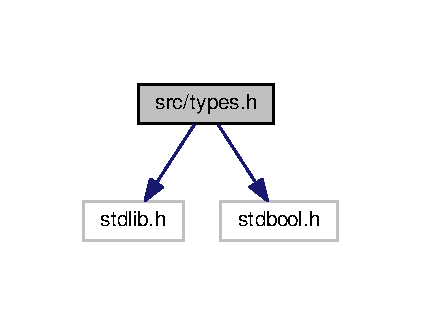
\includegraphics[width=145pt]{types_8h__incl}
\end{center}
\end{figure}
This graph shows which files directly or indirectly include this file\+:
\nopagebreak
\begin{figure}[H]
\begin{center}
\leavevmode
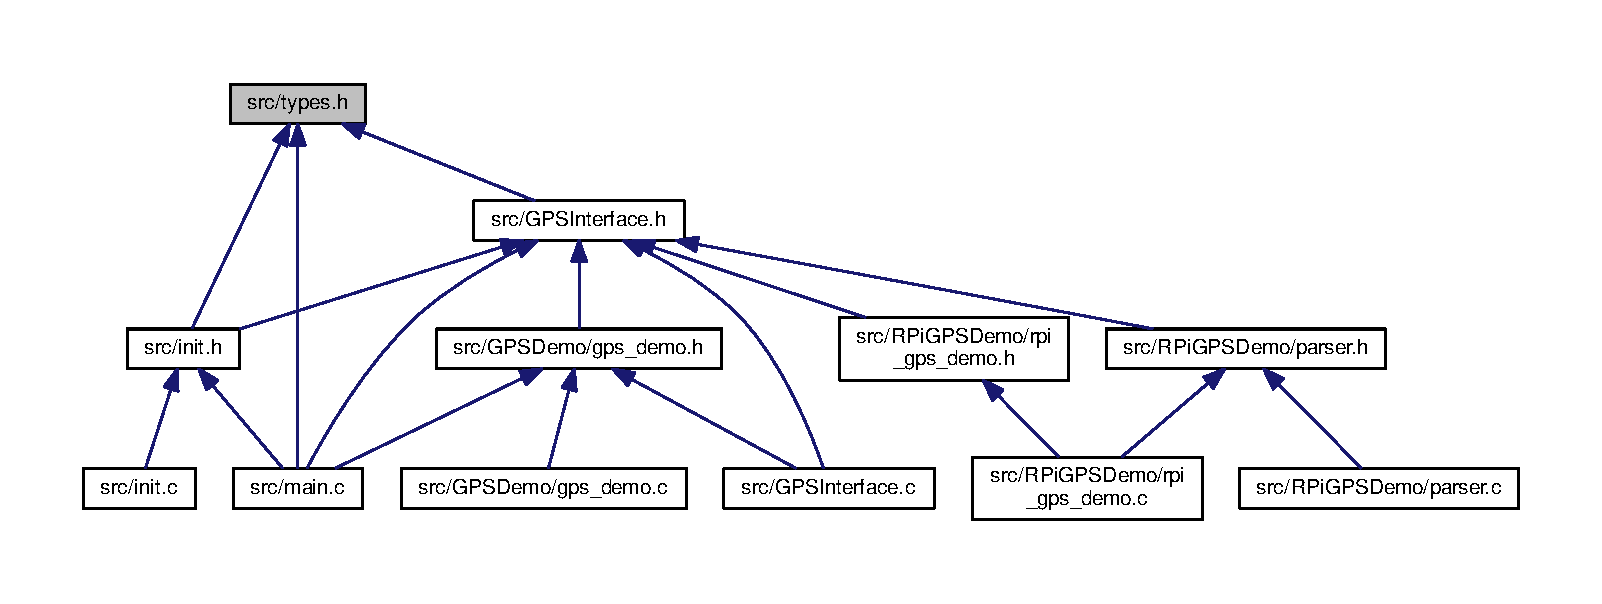
\includegraphics[width=350pt]{types_8h__dep__incl}
\end{center}
\end{figure}
\subsection*{Data Structures}
\begin{DoxyCompactItemize}
\item 
struct \hyperlink{struct_g_p_s_samp}{G\+P\+S\+Samp}
\begin{DoxyCompactList}\small\item\em Represents a smaller, truncated verion of the data gathered from G\+PS. \end{DoxyCompactList}\item 
struct \hyperlink{struct_g_e_o___point}{G\+E\+O\+\_\+\+Point}
\begin{DoxyCompactList}\small\item\em Represents a single 2D point. \end{DoxyCompactList}\item 
struct \hyperlink{struct_m_b_r}{M\+BR}
\begin{DoxyCompactList}\small\item\em Minimum bounding rectangle of a certain polygon. \end{DoxyCompactList}\item 
struct \hyperlink{struct_edge}{Edge}
\begin{DoxyCompactList}\small\item\em A straight line between two points. \end{DoxyCompactList}\item 
struct \hyperlink{struct_zone__general}{Zone\+\_\+general}
\begin{DoxyCompactList}\small\item\em Represents a single polygon. \end{DoxyCompactList}\item 
struct \hyperlink{struct_full_g_p_s_data}{Full\+G\+P\+S\+Data}
\begin{DoxyCompactList}\small\item\em The entire collection of relevant data, gathered from G\+PS. \end{DoxyCompactList}\item 
struct \hyperlink{structgga}{gga}
\begin{DoxyCompactList}\small\item\em Used to hold relevant data from \$\+G\+P\+G\+GA N\+M\+EA sentences from G\+PS. \end{DoxyCompactList}\item 
struct \hyperlink{structgsa}{gsa}
\begin{DoxyCompactList}\small\item\em Used to hold relevant data from \$\+G\+P\+G\+SA N\+M\+EA sentences from G\+PS. \end{DoxyCompactList}\item 
struct \hyperlink{structvtg}{vtg}
\begin{DoxyCompactList}\small\item\em Used to hold relevant data from \$\+G\+P\+V\+TG N\+M\+EA sentences from G\+PS. \end{DoxyCompactList}\item 
struct \hyperlink{structgll}{gll}
\begin{DoxyCompactList}\small\item\em Used to hold relevant data from \$\+G\+P\+G\+LL N\+M\+EA sentences from G\+PS. \end{DoxyCompactList}\item 
struct \hyperlink{structrmc}{rmc}
\begin{DoxyCompactList}\small\item\em Used to hold relevant data from \$\+G\+P\+R\+MC N\+M\+EA sentences from G\+PS. \end{DoxyCompactList}\end{DoxyCompactItemize}
\subsection*{Macros}
\begin{DoxyCompactItemize}
\item 
\#define \hyperlink{types_8h_a7e42e11a9434b785d263d129d887a36c}{O\+U\+T\+S\+I\+DE}~0
\item 
\#define \hyperlink{types_8h_a1a58ace3d61e5eddb10aaee57d9fcba9}{I\+N\+S\+I\+DE}~1
\item 
\#define \hyperlink{types_8h_ac4af596782111ed976bcf01f1f1027d3}{M\+I\+N\+\_\+\+A\+LT}~-\/500
\item 
\#define \hyperlink{types_8h_a93c97efc6e6ebd64ef14fefb0bbd9226}{M\+A\+X\+\_\+\+A\+LT}~10000
\end{DoxyCompactItemize}
\subsection*{Typedefs}
\begin{DoxyCompactItemize}
\item 
typedef unsigned char \hyperlink{types_8h_aba7bc1797add20fe3efdf37ced1182c5}{uint8\+\_\+t}
\end{DoxyCompactItemize}
\subsection*{Enumerations}
\begin{DoxyCompactItemize}
\item 
enum \hyperlink{types_8h_af6a258d8f3ee5206d682d799316314b1}{bool} \{ \hyperlink{types_8h_af6a258d8f3ee5206d682d799316314b1ae9de385ef6fe9bf3360d1038396b884c}{false}, 
\hyperlink{types_8h_af6a258d8f3ee5206d682d799316314b1a08f175a5505a10b9ed657defeb050e4b}{true}
 \}
\end{DoxyCompactItemize}


\subsection{Macro Definition Documentation}
\index{types.\+h@{types.\+h}!I\+N\+S\+I\+DE@{I\+N\+S\+I\+DE}}
\index{I\+N\+S\+I\+DE@{I\+N\+S\+I\+DE}!types.\+h@{types.\+h}}
\subsubsection[{\texorpdfstring{I\+N\+S\+I\+DE}{INSIDE}}]{\setlength{\rightskip}{0pt plus 5cm}\#define I\+N\+S\+I\+DE~1}\hypertarget{types_8h_a1a58ace3d61e5eddb10aaee57d9fcba9}{}\label{types_8h_a1a58ace3d61e5eddb10aaee57d9fcba9}
\index{types.\+h@{types.\+h}!M\+A\+X\+\_\+\+A\+LT@{M\+A\+X\+\_\+\+A\+LT}}
\index{M\+A\+X\+\_\+\+A\+LT@{M\+A\+X\+\_\+\+A\+LT}!types.\+h@{types.\+h}}
\subsubsection[{\texorpdfstring{M\+A\+X\+\_\+\+A\+LT}{MAX_ALT}}]{\setlength{\rightskip}{0pt plus 5cm}\#define M\+A\+X\+\_\+\+A\+LT~10000}\hypertarget{types_8h_a93c97efc6e6ebd64ef14fefb0bbd9226}{}\label{types_8h_a93c97efc6e6ebd64ef14fefb0bbd9226}
\index{types.\+h@{types.\+h}!M\+I\+N\+\_\+\+A\+LT@{M\+I\+N\+\_\+\+A\+LT}}
\index{M\+I\+N\+\_\+\+A\+LT@{M\+I\+N\+\_\+\+A\+LT}!types.\+h@{types.\+h}}
\subsubsection[{\texorpdfstring{M\+I\+N\+\_\+\+A\+LT}{MIN_ALT}}]{\setlength{\rightskip}{0pt plus 5cm}\#define M\+I\+N\+\_\+\+A\+LT~-\/500}\hypertarget{types_8h_ac4af596782111ed976bcf01f1f1027d3}{}\label{types_8h_ac4af596782111ed976bcf01f1f1027d3}
\index{types.\+h@{types.\+h}!O\+U\+T\+S\+I\+DE@{O\+U\+T\+S\+I\+DE}}
\index{O\+U\+T\+S\+I\+DE@{O\+U\+T\+S\+I\+DE}!types.\+h@{types.\+h}}
\subsubsection[{\texorpdfstring{O\+U\+T\+S\+I\+DE}{OUTSIDE}}]{\setlength{\rightskip}{0pt plus 5cm}\#define O\+U\+T\+S\+I\+DE~0}\hypertarget{types_8h_a7e42e11a9434b785d263d129d887a36c}{}\label{types_8h_a7e42e11a9434b785d263d129d887a36c}


\subsection{Typedef Documentation}
\index{types.\+h@{types.\+h}!uint8\+\_\+t@{uint8\+\_\+t}}
\index{uint8\+\_\+t@{uint8\+\_\+t}!types.\+h@{types.\+h}}
\subsubsection[{\texorpdfstring{uint8\+\_\+t}{uint8_t}}]{\setlength{\rightskip}{0pt plus 5cm}typedef unsigned char {\bf uint8\+\_\+t}}\hypertarget{types_8h_aba7bc1797add20fe3efdf37ced1182c5}{}\label{types_8h_aba7bc1797add20fe3efdf37ced1182c5}


\subsection{Enumeration Type Documentation}
\index{types.\+h@{types.\+h}!bool@{bool}}
\index{bool@{bool}!types.\+h@{types.\+h}}
\subsubsection[{\texorpdfstring{bool}{bool}}]{\setlength{\rightskip}{0pt plus 5cm}enum {\bf bool}}\hypertarget{types_8h_af6a258d8f3ee5206d682d799316314b1}{}\label{types_8h_af6a258d8f3ee5206d682d799316314b1}
\begin{Desc}
\item[Enumerator]\par
\begin{description}
\index{false@{false}!types.\+h@{types.\+h}}\index{types.\+h@{types.\+h}!false@{false}}\item[{\em 
false\hypertarget{types_8h_af6a258d8f3ee5206d682d799316314b1ae9de385ef6fe9bf3360d1038396b884c}{}\label{types_8h_af6a258d8f3ee5206d682d799316314b1ae9de385ef6fe9bf3360d1038396b884c}
}]\index{true@{true}!types.\+h@{types.\+h}}\index{types.\+h@{types.\+h}!true@{true}}\item[{\em 
true\hypertarget{types_8h_af6a258d8f3ee5206d682d799316314b1a08f175a5505a10b9ed657defeb050e4b}{}\label{types_8h_af6a258d8f3ee5206d682d799316314b1a08f175a5505a10b9ed657defeb050e4b}
}]\end{description}
\end{Desc}

\hypertarget{utils_8c}{}\section{src/utils.c File Reference}
\label{utils_8c}\index{src/utils.\+c@{src/utils.\+c}}
{\ttfamily \#include $<$string.\+h$>$}\\*
{\ttfamily \#include \char`\"{}utils.\+h\char`\"{}}\\*
{\ttfamily \#include \char`\"{}log\+Interface.\+h\char`\"{}}\\*
Include dependency graph for utils.\+c\+:
\nopagebreak
\begin{figure}[H]
\begin{center}
\leavevmode
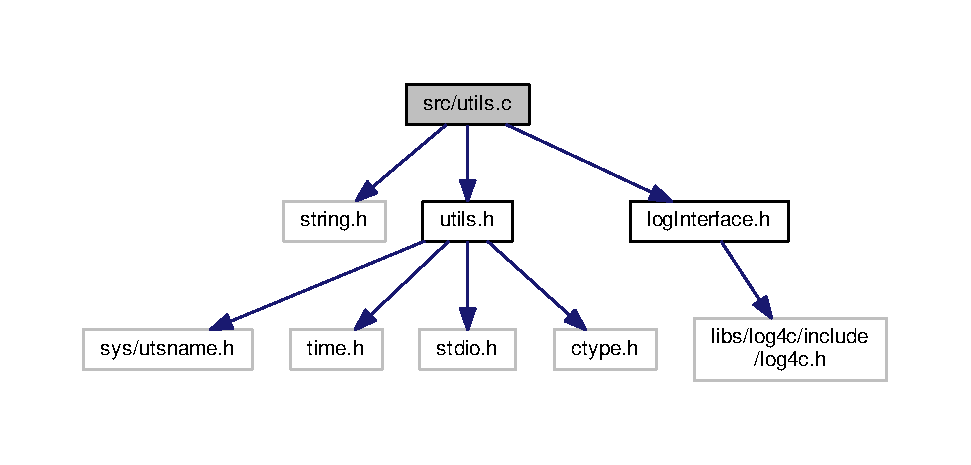
\includegraphics[width=350pt]{utils_8c__incl}
\end{center}
\end{figure}
\subsection*{Functions}
\begin{DoxyCompactItemize}
\item 
int \hyperlink{utils_8c_aab4b0b78fc58f681cda908bc549e2eb3}{suspend\+\_\+loop} (time\+\_\+t tv\+\_\+sec, long nsec)
\begin{DoxyCompactList}\small\item\em suspends the main loop for a specific time period, using nanosleep(). \end{DoxyCompactList}\item 
\hyperlink{utils_8h_ac172b6ea96d5e5322771db859ad1e65f}{platform\+\_\+id} \hyperlink{utils_8c_aa7805dae582961f7ef57afd9a420cfc7}{identify\+\_\+platform} (void)
\begin{DoxyCompactList}\small\item\em checks what platform we are on. \end{DoxyCompactList}\end{DoxyCompactItemize}


\subsection{Function Documentation}
\index{utils.\+c@{utils.\+c}!identify\+\_\+platform@{identify\+\_\+platform}}
\index{identify\+\_\+platform@{identify\+\_\+platform}!utils.\+c@{utils.\+c}}
\subsubsection[{\texorpdfstring{identify\+\_\+platform(void)}{identify_platform(void)}}]{\setlength{\rightskip}{0pt plus 5cm}{\bf platform\+\_\+id} identify\+\_\+platform (
\begin{DoxyParamCaption}
\item[{void}]{}
\end{DoxyParamCaption}
)}\hypertarget{utils_8c_aa7805dae582961f7ef57afd9a420cfc7}{}\label{utils_8c_aa7805dae582961f7ef57afd9a420cfc7}


checks what platform we are on. 

\begin{DoxyReturn}{Returns}
returns the id of the platform. one if the values of the platform\+\_\+id enum. 
\end{DoxyReturn}
\index{utils.\+c@{utils.\+c}!suspend\+\_\+loop@{suspend\+\_\+loop}}
\index{suspend\+\_\+loop@{suspend\+\_\+loop}!utils.\+c@{utils.\+c}}
\subsubsection[{\texorpdfstring{suspend\+\_\+loop(time\+\_\+t tv\+\_\+sec, long nsec)}{suspend_loop(time_t tv_sec, long nsec)}}]{\setlength{\rightskip}{0pt plus 5cm}int suspend\+\_\+loop (
\begin{DoxyParamCaption}
\item[{time\+\_\+t}]{tv\+\_\+sec, }
\item[{long}]{nsec}
\end{DoxyParamCaption}
)}\hypertarget{utils_8c_aab4b0b78fc58f681cda908bc549e2eb3}{}\label{utils_8c_aab4b0b78fc58f681cda908bc549e2eb3}


suspends the main loop for a specific time period, using nanosleep(). 


\begin{DoxyParams}[1]{Parameters}
\mbox{\tt in}  & {\em tv\+\_\+sec} & first value of \textquotesingle{}struct timespec\textquotesingle{}, storing the seconds. \\
\hline
\mbox{\tt in}  & {\em nsec} & second value of \textquotesingle{}struct timespec\textquotesingle{} storing the nanoseconds. \\
\hline
\end{DoxyParams}
\begin{DoxyReturn}{Returns}
returns the rv of nanosleep() 
\end{DoxyReturn}

\hypertarget{utils_8d}{}\section{src/utils.d File Reference}
\label{utils_8d}\index{src/utils.\+d@{src/utils.\+d}}

\hypertarget{utils_8h}{}\section{src/utils.h File Reference}
\label{utils_8h}\index{src/utils.\+h@{src/utils.\+h}}
{\ttfamily \#include $<$sys/utsname.\+h$>$}\\*
{\ttfamily \#include $<$time.\+h$>$}\\*
{\ttfamily \#include $<$stdio.\+h$>$}\\*
{\ttfamily \#include $<$ctype.\+h$>$}\\*
Include dependency graph for utils.\+h\+:
\nopagebreak
\begin{figure}[H]
\begin{center}
\leavevmode
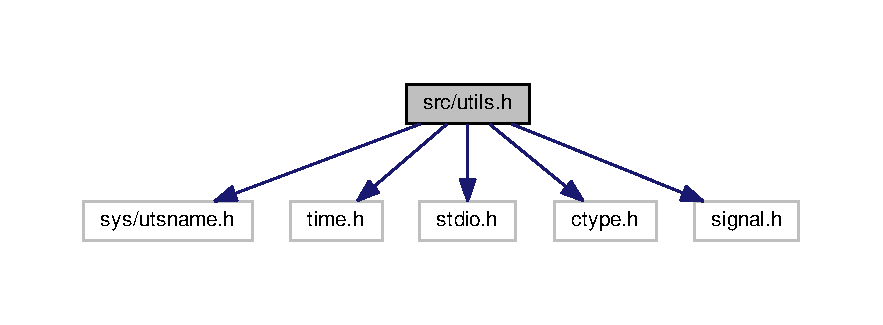
\includegraphics[width=350pt]{utils_8h__incl}
\end{center}
\end{figure}
This graph shows which files directly or indirectly include this file\+:
\nopagebreak
\begin{figure}[H]
\begin{center}
\leavevmode
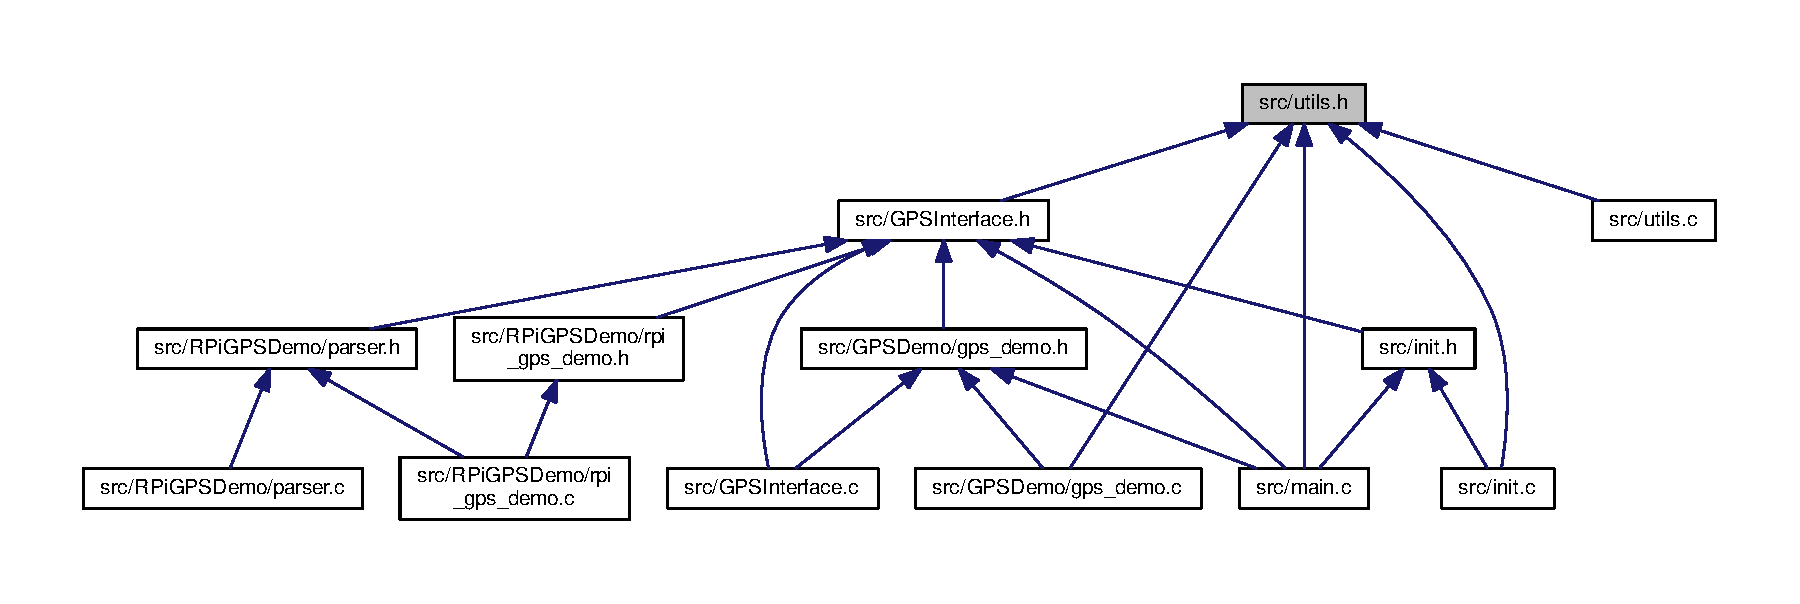
\includegraphics[width=350pt]{utils_8h__dep__incl}
\end{center}
\end{figure}
\subsection*{Macros}
\begin{DoxyCompactItemize}
\item 
\#define \hyperlink{utils_8h_affe776513b24d84b39af8ab0930fef7f}{max}(a,  b)~(((a) $>$ (b)) ? (a) \+: (b))
\item 
\#define \hyperlink{utils_8h_ac6afabdc09a49a433ee19d8a9486056d}{min}(a,  b)~(((a) $<$ (b)) ? (a) \+: (b))
\item 
\#define \hyperlink{utils_8h_aee09ac526ce597d7f2e91c0bea6de514}{range\+\_\+valid}(x,  lo,  hi)~( ((x $>$= lo) \&\& (x $<$= hi)) ) ? 1 \+: 0
\item 
\#define \hyperlink{utils_8h_a598a3330b3c21701223ee0ca14316eca}{PI}~3.\+14159265
\item 
\#define \hyperlink{utils_8h_a07484107e6d9fdf38b53edf631d6511d}{E}~2.\+71828182
\item 
\#define \hyperlink{utils_8h_ae77b2eba6114f88a6407fb709d71f187}{T\+I\+M\+E\+\_\+\+T\+O\+\_\+\+W\+A\+I\+T\+\_\+\+S\+EC}~1
\item 
\#define \hyperlink{utils_8h_aa69480d2c7183cc7357453e7d25a6e31}{T\+I\+M\+E\+\_\+\+T\+O\+\_\+\+W\+A\+I\+T\+\_\+\+N\+S\+EC}~0
\item 
\#define \hyperlink{utils_8h_a9258c030cce8027f0020e7a0a452c859}{M\+A\+X\+\_\+\+N\+M\+E\+A\+\_\+\+M\+S\+G\+\_\+\+S\+I\+ZE}~83
\item 
\#define \hyperlink{utils_8h_a2428561553d92d6622e85e4bb693c13c}{T\+O\+L\+E\+R\+A\+T\+E\+S\+\_\+\+I\+N\+T\+E\+R\+R\+U\+PT}~1
\item 
\#define \hyperlink{utils_8h_a46b83d9f6c23b1b65a8cecfd775ddaed}{E\+I\+N\+TR}~-\/1
\end{DoxyCompactItemize}
\subsection*{Enumerations}
\begin{DoxyCompactItemize}
\item 
enum \hyperlink{utils_8h_ac172b6ea96d5e5322771db859ad1e65f}{platform\+\_\+id} \{ \hyperlink{utils_8h_ac172b6ea96d5e5322771db859ad1e65fa8e0da7a705cf9d08ebffe49c0c8441d9}{U\+N\+K\+N\+O\+W\+N\+\_\+\+P\+L\+A\+T\+F\+O\+RM}, 
\hyperlink{utils_8h_ac172b6ea96d5e5322771db859ad1e65fa03b7f32fb426197602cbdf872eb289b3}{X86}, 
\hyperlink{utils_8h_ac172b6ea96d5e5322771db859ad1e65fa3a92c0053fe92a134da3e6a82ea1adb6}{A\+RM}
 \}
\end{DoxyCompactItemize}
\subsection*{Functions}
\begin{DoxyCompactItemize}
\item 
\hyperlink{utils_8h_ac172b6ea96d5e5322771db859ad1e65f}{platform\+\_\+id} \hyperlink{utils_8h_aa7805dae582961f7ef57afd9a420cfc7}{identify\+\_\+platform} (void)
\begin{DoxyCompactList}\small\item\em checks what platform we are on. \end{DoxyCompactList}\item 
int \hyperlink{utils_8h_aab4b0b78fc58f681cda908bc549e2eb3}{suspend\+\_\+loop} (time\+\_\+t tv\+\_\+sec, long nsec)
\begin{DoxyCompactList}\small\item\em suspends the main loop for a specific time period, using nanosleep(). \end{DoxyCompactList}\end{DoxyCompactItemize}


\subsection{Macro Definition Documentation}
\index{utils.\+h@{utils.\+h}!E@{E}}
\index{E@{E}!utils.\+h@{utils.\+h}}
\subsubsection[{\texorpdfstring{E}{E}}]{\setlength{\rightskip}{0pt plus 5cm}\#define E~2.\+71828182}\hypertarget{utils_8h_a07484107e6d9fdf38b53edf631d6511d}{}\label{utils_8h_a07484107e6d9fdf38b53edf631d6511d}
\index{utils.\+h@{utils.\+h}!E\+I\+N\+TR@{E\+I\+N\+TR}}
\index{E\+I\+N\+TR@{E\+I\+N\+TR}!utils.\+h@{utils.\+h}}
\subsubsection[{\texorpdfstring{E\+I\+N\+TR}{EINTR}}]{\setlength{\rightskip}{0pt plus 5cm}\#define E\+I\+N\+TR~-\/1}\hypertarget{utils_8h_a46b83d9f6c23b1b65a8cecfd775ddaed}{}\label{utils_8h_a46b83d9f6c23b1b65a8cecfd775ddaed}
\index{utils.\+h@{utils.\+h}!max@{max}}
\index{max@{max}!utils.\+h@{utils.\+h}}
\subsubsection[{\texorpdfstring{max}{max}}]{\setlength{\rightskip}{0pt plus 5cm}\#define max(
\begin{DoxyParamCaption}
\item[{}]{a, }
\item[{}]{b}
\end{DoxyParamCaption}
)~(((a) $>$ (b)) ? (a) \+: (b))}\hypertarget{utils_8h_affe776513b24d84b39af8ab0930fef7f}{}\label{utils_8h_affe776513b24d84b39af8ab0930fef7f}
\index{utils.\+h@{utils.\+h}!M\+A\+X\+\_\+\+N\+M\+E\+A\+\_\+\+M\+S\+G\+\_\+\+S\+I\+ZE@{M\+A\+X\+\_\+\+N\+M\+E\+A\+\_\+\+M\+S\+G\+\_\+\+S\+I\+ZE}}
\index{M\+A\+X\+\_\+\+N\+M\+E\+A\+\_\+\+M\+S\+G\+\_\+\+S\+I\+ZE@{M\+A\+X\+\_\+\+N\+M\+E\+A\+\_\+\+M\+S\+G\+\_\+\+S\+I\+ZE}!utils.\+h@{utils.\+h}}
\subsubsection[{\texorpdfstring{M\+A\+X\+\_\+\+N\+M\+E\+A\+\_\+\+M\+S\+G\+\_\+\+S\+I\+ZE}{MAX_NMEA_MSG_SIZE}}]{\setlength{\rightskip}{0pt plus 5cm}\#define M\+A\+X\+\_\+\+N\+M\+E\+A\+\_\+\+M\+S\+G\+\_\+\+S\+I\+ZE~83}\hypertarget{utils_8h_a9258c030cce8027f0020e7a0a452c859}{}\label{utils_8h_a9258c030cce8027f0020e7a0a452c859}
\index{utils.\+h@{utils.\+h}!min@{min}}
\index{min@{min}!utils.\+h@{utils.\+h}}
\subsubsection[{\texorpdfstring{min}{min}}]{\setlength{\rightskip}{0pt plus 5cm}\#define min(
\begin{DoxyParamCaption}
\item[{}]{a, }
\item[{}]{b}
\end{DoxyParamCaption}
)~(((a) $<$ (b)) ? (a) \+: (b))}\hypertarget{utils_8h_ac6afabdc09a49a433ee19d8a9486056d}{}\label{utils_8h_ac6afabdc09a49a433ee19d8a9486056d}
\index{utils.\+h@{utils.\+h}!PI@{PI}}
\index{PI@{PI}!utils.\+h@{utils.\+h}}
\subsubsection[{\texorpdfstring{PI}{PI}}]{\setlength{\rightskip}{0pt plus 5cm}\#define PI~3.\+14159265}\hypertarget{utils_8h_a598a3330b3c21701223ee0ca14316eca}{}\label{utils_8h_a598a3330b3c21701223ee0ca14316eca}
\index{utils.\+h@{utils.\+h}!range\+\_\+valid@{range\+\_\+valid}}
\index{range\+\_\+valid@{range\+\_\+valid}!utils.\+h@{utils.\+h}}
\subsubsection[{\texorpdfstring{range\+\_\+valid}{range_valid}}]{\setlength{\rightskip}{0pt plus 5cm}\#define range\+\_\+valid(
\begin{DoxyParamCaption}
\item[{}]{x, }
\item[{}]{lo, }
\item[{}]{hi}
\end{DoxyParamCaption}
)~( ((x $>$= lo) \&\& (x $<$= hi)) ) ? 1 \+: 0}\hypertarget{utils_8h_aee09ac526ce597d7f2e91c0bea6de514}{}\label{utils_8h_aee09ac526ce597d7f2e91c0bea6de514}
\index{utils.\+h@{utils.\+h}!T\+I\+M\+E\+\_\+\+T\+O\+\_\+\+W\+A\+I\+T\+\_\+\+N\+S\+EC@{T\+I\+M\+E\+\_\+\+T\+O\+\_\+\+W\+A\+I\+T\+\_\+\+N\+S\+EC}}
\index{T\+I\+M\+E\+\_\+\+T\+O\+\_\+\+W\+A\+I\+T\+\_\+\+N\+S\+EC@{T\+I\+M\+E\+\_\+\+T\+O\+\_\+\+W\+A\+I\+T\+\_\+\+N\+S\+EC}!utils.\+h@{utils.\+h}}
\subsubsection[{\texorpdfstring{T\+I\+M\+E\+\_\+\+T\+O\+\_\+\+W\+A\+I\+T\+\_\+\+N\+S\+EC}{TIME_TO_WAIT_NSEC}}]{\setlength{\rightskip}{0pt plus 5cm}\#define T\+I\+M\+E\+\_\+\+T\+O\+\_\+\+W\+A\+I\+T\+\_\+\+N\+S\+EC~0}\hypertarget{utils_8h_aa69480d2c7183cc7357453e7d25a6e31}{}\label{utils_8h_aa69480d2c7183cc7357453e7d25a6e31}
\index{utils.\+h@{utils.\+h}!T\+I\+M\+E\+\_\+\+T\+O\+\_\+\+W\+A\+I\+T\+\_\+\+S\+EC@{T\+I\+M\+E\+\_\+\+T\+O\+\_\+\+W\+A\+I\+T\+\_\+\+S\+EC}}
\index{T\+I\+M\+E\+\_\+\+T\+O\+\_\+\+W\+A\+I\+T\+\_\+\+S\+EC@{T\+I\+M\+E\+\_\+\+T\+O\+\_\+\+W\+A\+I\+T\+\_\+\+S\+EC}!utils.\+h@{utils.\+h}}
\subsubsection[{\texorpdfstring{T\+I\+M\+E\+\_\+\+T\+O\+\_\+\+W\+A\+I\+T\+\_\+\+S\+EC}{TIME_TO_WAIT_SEC}}]{\setlength{\rightskip}{0pt plus 5cm}\#define T\+I\+M\+E\+\_\+\+T\+O\+\_\+\+W\+A\+I\+T\+\_\+\+S\+EC~1}\hypertarget{utils_8h_ae77b2eba6114f88a6407fb709d71f187}{}\label{utils_8h_ae77b2eba6114f88a6407fb709d71f187}
\index{utils.\+h@{utils.\+h}!T\+O\+L\+E\+R\+A\+T\+E\+S\+\_\+\+I\+N\+T\+E\+R\+R\+U\+PT@{T\+O\+L\+E\+R\+A\+T\+E\+S\+\_\+\+I\+N\+T\+E\+R\+R\+U\+PT}}
\index{T\+O\+L\+E\+R\+A\+T\+E\+S\+\_\+\+I\+N\+T\+E\+R\+R\+U\+PT@{T\+O\+L\+E\+R\+A\+T\+E\+S\+\_\+\+I\+N\+T\+E\+R\+R\+U\+PT}!utils.\+h@{utils.\+h}}
\subsubsection[{\texorpdfstring{T\+O\+L\+E\+R\+A\+T\+E\+S\+\_\+\+I\+N\+T\+E\+R\+R\+U\+PT}{TOLERATES_INTERRUPT}}]{\setlength{\rightskip}{0pt plus 5cm}\#define T\+O\+L\+E\+R\+A\+T\+E\+S\+\_\+\+I\+N\+T\+E\+R\+R\+U\+PT~1}\hypertarget{utils_8h_a2428561553d92d6622e85e4bb693c13c}{}\label{utils_8h_a2428561553d92d6622e85e4bb693c13c}


\subsection{Enumeration Type Documentation}
\index{utils.\+h@{utils.\+h}!platform\+\_\+id@{platform\+\_\+id}}
\index{platform\+\_\+id@{platform\+\_\+id}!utils.\+h@{utils.\+h}}
\subsubsection[{\texorpdfstring{platform\+\_\+id}{platform_id}}]{\setlength{\rightskip}{0pt plus 5cm}enum {\bf platform\+\_\+id}}\hypertarget{utils_8h_ac172b6ea96d5e5322771db859ad1e65f}{}\label{utils_8h_ac172b6ea96d5e5322771db859ad1e65f}
\begin{Desc}
\item[Enumerator]\par
\begin{description}
\index{U\+N\+K\+N\+O\+W\+N\+\_\+\+P\+L\+A\+T\+F\+O\+RM@{U\+N\+K\+N\+O\+W\+N\+\_\+\+P\+L\+A\+T\+F\+O\+RM}!utils.\+h@{utils.\+h}}\index{utils.\+h@{utils.\+h}!U\+N\+K\+N\+O\+W\+N\+\_\+\+P\+L\+A\+T\+F\+O\+RM@{U\+N\+K\+N\+O\+W\+N\+\_\+\+P\+L\+A\+T\+F\+O\+RM}}\item[{\em 
U\+N\+K\+N\+O\+W\+N\+\_\+\+P\+L\+A\+T\+F\+O\+RM\hypertarget{utils_8h_ac172b6ea96d5e5322771db859ad1e65fa8e0da7a705cf9d08ebffe49c0c8441d9}{}\label{utils_8h_ac172b6ea96d5e5322771db859ad1e65fa8e0da7a705cf9d08ebffe49c0c8441d9}
}]\index{X86@{X86}!utils.\+h@{utils.\+h}}\index{utils.\+h@{utils.\+h}!X86@{X86}}\item[{\em 
X86\hypertarget{utils_8h_ac172b6ea96d5e5322771db859ad1e65fa03b7f32fb426197602cbdf872eb289b3}{}\label{utils_8h_ac172b6ea96d5e5322771db859ad1e65fa03b7f32fb426197602cbdf872eb289b3}
}]\index{A\+RM@{A\+RM}!utils.\+h@{utils.\+h}}\index{utils.\+h@{utils.\+h}!A\+RM@{A\+RM}}\item[{\em 
A\+RM\hypertarget{utils_8h_ac172b6ea96d5e5322771db859ad1e65fa3a92c0053fe92a134da3e6a82ea1adb6}{}\label{utils_8h_ac172b6ea96d5e5322771db859ad1e65fa3a92c0053fe92a134da3e6a82ea1adb6}
}]\end{description}
\end{Desc}


\subsection{Function Documentation}
\index{utils.\+h@{utils.\+h}!identify\+\_\+platform@{identify\+\_\+platform}}
\index{identify\+\_\+platform@{identify\+\_\+platform}!utils.\+h@{utils.\+h}}
\subsubsection[{\texorpdfstring{identify\+\_\+platform(void)}{identify_platform(void)}}]{\setlength{\rightskip}{0pt plus 5cm}{\bf platform\+\_\+id} identify\+\_\+platform (
\begin{DoxyParamCaption}
\item[{void}]{}
\end{DoxyParamCaption}
)}\hypertarget{utils_8h_aa7805dae582961f7ef57afd9a420cfc7}{}\label{utils_8h_aa7805dae582961f7ef57afd9a420cfc7}


checks what platform we are on. 

\begin{DoxyReturn}{Returns}
returns the id of the platform. one if the values of the platform\+\_\+id enum. 
\end{DoxyReturn}
\index{utils.\+h@{utils.\+h}!suspend\+\_\+loop@{suspend\+\_\+loop}}
\index{suspend\+\_\+loop@{suspend\+\_\+loop}!utils.\+h@{utils.\+h}}
\subsubsection[{\texorpdfstring{suspend\+\_\+loop(time\+\_\+t tv\+\_\+sec, long nsec)}{suspend_loop(time_t tv_sec, long nsec)}}]{\setlength{\rightskip}{0pt plus 5cm}int suspend\+\_\+loop (
\begin{DoxyParamCaption}
\item[{time\+\_\+t}]{tv\+\_\+sec, }
\item[{long}]{nsec}
\end{DoxyParamCaption}
)}\hypertarget{utils_8h_aab4b0b78fc58f681cda908bc549e2eb3}{}\label{utils_8h_aab4b0b78fc58f681cda908bc549e2eb3}


suspends the main loop for a specific time period, using nanosleep(). 


\begin{DoxyParams}[1]{Parameters}
\mbox{\tt in}  & {\em tv\+\_\+sec} & first value of \textquotesingle{}struct timespec\textquotesingle{}, storing the seconds. \\
\hline
\mbox{\tt in}  & {\em nsec} & second value of \textquotesingle{}struct timespec\textquotesingle{} storing the nanoseconds. \\
\hline
\end{DoxyParams}
\begin{DoxyReturn}{Returns}
returns the rv of nanosleep() 
\end{DoxyReturn}

%--- End generated contents ---

% Index
\backmatter
\newpage
\phantomsection
\clearemptydoublepage
\addcontentsline{toc}{chapter}{Index}
\printindex

\end{document}
